% Authors:  Nils Carqueville, Daniel Murfet

% TODO: References are to arXiv version of [KR]

\documentclass{compositio}
\usepackage{stmaryrd}
\usepackage{amsmath, amscd, amssymb, mathrsfs, accents, amsfonts}
\usepackage{url}
\usepackage[all]{xy}
\usepackage{longtable}
\usepackage{dsfont}
\usepackage{tikz}
\def\nicenocolourscheme{\shadedraw[top color=gray!2, bottom color=gray!25, draw=gray!50!black, dashed]}
\definecolor{Myblue}{rgb}{0,0,0.6}
\usepackage[a4paper,colorlinks,citecolor=Myblue,linkcolor=Myblue,urlcolor=Myblue,pdfpagemode=None]{hyperref}

\SelectTips{cm}{}

\newtheorem{theorem}{Theorem}[section]
\newtheorem{proposition}[theorem]{Proposition}
\newtheorem{lemma}[theorem]{Lemma}
\newtheorem{corollary}[theorem]{Corollary}
\newtheorem*{theoremn}{Theorem}

\theoremstyle{definition}
\newtheorem{definition}[theorem]{Definition}
\newtheorem{example}[theorem]{Example}
\newtheorem{remark}[theorem]{Remark}
\newtheorem{s}[theorem]{}
\newtheorem*{setup}{Setup}
\newtheorem*{propositionn}{Proposition}

\numberwithin{equation}{section}

% Operators
\def\eval{\operatorname{ev}}
\def\res{\operatorname{Res}}
\def\sg{\operatorname{sg}}
\def\Inj{\operatorname{Inj}}
\def\inc{\operatorname{inc}}
\def\Proj{\operatorname{Proj}}
\def\Coker{\operatorname{Coker}}
\def\Ker{\operatorname{Ker}}
\def\Im{\operatorname{Im}}
\def\free{\operatorname{free}}
\def\can{\operatorname{can}}
\def\ac{\operatorname{ac}}
\def\HH{\operatorname{HH}}
\def\K{\mathbf{K}}
\def\D{\mathbf{D}}
\def\N{\mathbf{N}}
\def\sing{\operatorname{Sg}}
\def\Hom{\operatorname{Hom}}
\def\uHom{\underline{\Hom}}
\def\modd{\operatorname{mod}}
\def\Modd{\operatorname{Mod}}
\def\Grmodd{\operatorname{GrMod}}
\def\CM{\operatorname{CM}}
\def\Ker{\operatorname{Ker}}
\def\Spec{\operatorname{Spec}}
\def\straightK{\operatorname{K}}
\def\straightC{\operatorname{C}}
\def\holim{\operatorname{hocolim}}
\DeclareMathOperator{\Ext}{Ext}
\DeclareMathOperator{\coh}{coh}
\DeclareMathOperator{\serre}{S}
\DeclareMathOperator{\Flat}{Flat}
\DeclareMathOperator{\qc}{qc}
\DeclareMathOperator{\Perf}{Perf}
\DeclareMathOperator{\Map}{Map}
\DeclareMathOperator{\Qco}{Qco}
\DeclareMathOperator{\Tr}{Tr}
\DeclareMathOperator{\End}{End}
\DeclareMathOperator{\rank}{rank}
\DeclareMathOperator{\tot}{Tot}
\DeclareMathOperator{\skos}{K}
\DeclareMathOperator{\hht}{ht}
\DeclareMathOperator{\depth}{depth}
\DeclareMathOperator{\STr}{STr}
\DeclareMathOperator{\tr}{tr}
\DeclareMathOperator{\ch}{ch}
\DeclareMathOperator{\str}{str}
\DeclareMathOperator{\hmf}{hmf}
\DeclareMathOperator{\HMF}{HMF}
\DeclareMathOperator{\HF}{HF}
\DeclareMathOperator{\pr}{pr}
\DeclareMathOperator{\At}{At}
\DeclareMathOperator{\mff}{mf}
\DeclareMathOperator{\MF}{MF}

\begin{document}

% Commands
\def\dbsing{\mathbf{D}_{\sing}}
\def\dbsinge{\mathbf{D}'_{\sing}}
\def\dcpx{D}
\def\trans{\tau}
\def\Res{\res\!}
\newcommand{\Ress}[1]{\res_{#1}\!}
\newcommand{\kosz}[1]{E[#1]}
\newcommand{\ud}{\mathrm{d}}
\newcommand{\kflat}[1]{\K(\Flat #1)}
\newcommand{\kflatl}[2]{\K_{#1}(\Flat #2)}
\newcommand{\koszul}[2]{\operatorname{E}[#1]}
\newcommand{\ukoszul}[2]{\straightK[#1]}
\newcommand{\cech}[2]{\check{\straightC}[#1]}
\newcommand{\cat}[1]{\mathcal{#1}}
\newcommand{\qder}[1]{\mathbf{D}(#1)}
\newcommand{\qderl}[2]{\mathbf{D}_{#1}(#2)}
\newcommand{\qderu}[2]{\mathbf{D}^{#1}(#2)}
\newcommand{\lto}{\longrightarrow}
\newcommand{\xlto}[1]{\stackrel{#1}\lto}
\newcommand{\mf}[1]{\mathfrak{#1}}
\newcommand{\md}[1]{\mathscr{#1}}
\newcommand{\kinj}[1]{\K(\Inj #1)}
\newcommand{\kinju}[2]{\K^{#1}(\Inj #2)}
\newcommand{\kinjl}[2]{\K_{#1}(\Inj #2)}
\newcommand{\kprof}[1]{\mathbf{N}(\Flat #1)}
\newcommand{\kprofu}[2]{\mathbf{N}^{#1}(\Flat #2)}
\newcommand{\kprofl}[2]{\mathbf{N}_{#1}(\Flat #2)}
\newcommand{\kproful}[3]{\mathbf{N}^{#1}_{#2}(\Flat #3)}
\newcommand{\homd}[2]{[#1,#2]_{\mathbb{D}}}
\newcommand{\homk}[2]{[#1,#2]_{\mathbb{K}}}
\newcommand{\homn}[2]{[#1,#2]_{\mathds{N}}}
\newcommand{\lift}[1]{\dot{#1}}
\newcommand{\dlift}[1]{\ddot{#1}}
\def\qhom{\mathscr{H}\! om_{\qc}}
\def\rdev{\mathds{R}}
\def\dual{*}
\def\uotimes{\underaccent{\;\;\:=}{\otimes}}
\newcommand{\qcmod}[1]{\Qco(#1)}
\def\shom{\operatorname{Hom}}
\def\l{\,|\,}
\def\sgn{\textup{sgn}}
\def\nablagr{\nabla_{\operatorname{gr}}}
\newcommand{\kproj}[1]{\K(\Proj #1)}
\newcommand{\kprojl}[2]{\K_{#1}(\Proj #2)}
\newcommand{\kproju}[2]{\K^{#1}(\Proj #2)}
\newcommand{\kprojul}[3]{\K^{#1}_{#2}(\Proj #3)}
\def\dpart{\mathbb{D}}
\def\homot{\simeq}
\def\ceta{\vartheta}
\def\ctr{\Tr^{\sg}}
\def\cf{\boldsymbol{cf}}
\def\bx{\boldsymbol{x}}
\def\by{\boldsymbol{y}}
\def\ba{\boldsymbol{a}}
\def\bb{\boldsymbol{b}}
\def\totimes{\otimes}
\def\di{Q}
\def\rint{R_{\text{int}}}
\def\rext{R_{\text{ext}}}
\def\intvar{n}
\newcommand{\cotimes}[1]{\,\widehat{\otimes}_{#1}\,}
\def\QQ{\mathds{Q}}
\def\krc{C}
\def\diffm{d}
\def\diffh{d_{\chi}}
\def\redh{\overline{H}}
\def\ZZ{\mathds{Z}}
\def\bs{\boldsymbol}
\def\Ztwo{\mathds{Z}_2}
\def\mdual{^{\vee}}
\def\KR{\operatorname{KR}}
\def\I{\!\operatorname{i}\!}
\def\E{\operatorname{e}\!}
\def\sln{\mathfrak{sl}(N)}
\def\nN{\mathds{N}}
\def\nZ{\mathds{Z}}
\def\nQ{\mathds{Q}}
\def\nR{\mathds{R}}
\def\nC{\mathds{C}}
\def\idem{\varepsilon}
\def\Xcirc{%
\begin{tikzpicture}[inner sep=0mm]
\node (X) at (0,0) {$X$};
\node (0) at (0,0) [circle,inner sep=0.99pt, thin,draw=black,fill= white] {};
\end{tikzpicture}%
}
\def\Xbul{%
\begin{tikzpicture}[inner sep=0mm]
\node (X) at (0,0) {$X$};
\node (0) at (0,0) [circle,inner sep=0.99pt, thin,draw=black,fill= black] {};
\end{tikzpicture}%
}
\def\id{\operatorname{id}}


\title{Computing Khovanov-Rozansky homology \\ and defect fusion}
\author{Nils Carqueville}
\email{nils.carqueville@physik.uni-muenchen.de}
\address{Arnold Sommerfeld Center for Theoretical Physics, LMU M\"unchen \& Excellence Cluster Universe}

\author{Daniel Murfet}
\email{daniel.murfet@math.ucla.edu}
\address{Department of Mathematics, UCLA}

\classification{TODO}

\begin{abstract}
We compute the categorified $\sln$ link invariants as defined by Khovanov and Rozansky, for various links and various values of~$N$. This direct computation is made tractable by a general and constructive method to reduce tensor products of matrix factorisations to finite rank, which also has an interpretation as fusion of defect operators in B-twisted Landau-Ginzburg models. We implement this method on the computer and show how to use it in practice. 
\end{abstract}

\maketitle

\section{Introduction}

In this paper we present and implement the first method to directly compute Khovanov and Rozansky's categorified $\sln$ link invariants for arbitrary links. This is made possible by a technology to explicitly fuse topological defects in Landau-Ginzburg models. In the following we shall explain how these two topics relate, try to put them into context, and outline the main results of the present paper. 

Let us begin by recalling some pieces of knot theory at the borderland of pure mathematics and mathematical physics. By knot theory we mean the study of isotopy classes of knotted and linked circles in $S^3$. One way to try and distinguish two given links is to compare their polynomial invariants like the Jones and Homfly polynomials~\cite{JonesPolynomialPaper, Homfly, HomflyPT}. Such invariants can be computed from the essentially \emph{two}-dimensional link diagram and the skein relations. 

In the seminal work~\cite{wittenjones} it was explained how one can understand and compute such invariants as path integrals in a \emph{three}-dimensional topological field theory. More precisely, this theory is Chern-Simons theory, and the computability of link invariants in this framework is afforded by a relation to two-dimensional rational conformal field theories. These ideas and results together with those of~\cite{t1988YB} were formalised in~\cite{RT1990, RT1991, turaevbook} to produce link invariants from any modular tensor category (which is the representation category of the associated vertex operator algebra in the case of Chern-Simons theory). 

The ways in which Chern-Simons theory is related to various other fields are by far not limited to the situation just mentioned. In particular, Chern-Simons theory on $S^3$ is also the open string field theory for A-type topological string theory on $T^*S^3$~\cite{w9207094}. This together with ideas from gauge/gravity duality and connections to M-theory lead to very successful proposals to effectively compute polynomial link invariants from topological string amplitudes and BPS state counting~\cite{gv9811131, ov9912123, lmv0010102}; see~\cite{marinoknotbook} for a review of much of the string theoretic story. 

\medskip

In a parallel development, the application of the categorification programme to link invariants was initiated in~\cite{cf9405183} and carried out for the Jones polynomial in~\cite{k9908171}. Very roughly, the idea is to refine the construction of an invariant in a systematic manner, hoping to produce a more effective way to distinguish links. 

It is easy to give a precise definition of the notion of categorification of some mathematical structure~$S$. It is nothing but a category~$\mathcal C$ together with a map~$f$ from the isomorphism classes of objects of~$\mathcal C$ to~$S$. A standard example is the case of $S=\nN$ where~$\mathcal C$ is the category of vector spaces and~$f$ simply assigns the dimension. Another example, which will be central for us, is where one categorifies the space~$S$ of Laurent polynomials (interpreted as link invariants) by constructing a category~$\mathcal C$ of graded complexes, and the map $f:\operatorname{Isom}(\mathcal C)\longrightarrow S$ is given by computing the Poincar\'e polynomial. 

A categorification of the $\sln$ link invariants was achieved by Khovanov and Rozansky in~\cite{kr0401268}. It is these homological link invariants that we study and compute in the present paper. Before we give an overview of the construction and our results, let us briefly go on to embed them into the context of further recent developments. 

Following~\cite{kr0401268}, which reproduces Khovanov homology in the special case $N=2$, categorifications of the Homfly and Kauffman polynomials were proposed in~\cite{kr0505056, kr0701333}, and in~\cite{y0906.0220, w0907.0695} the $\sln$ categorification was extended to the case where arbitrary exterior powers of the defining representation label the link components. In all the works just mentioned matrix factorisations play a central role, but this is only one of many approaches to categorified link invariants. In particular, there are constructions of categorified $\sln$ link invariants via the category~$\mathcal O$~\cite{sCatTLcTCpf, ms0709.1971, s0701045}, via Floer homology~\cite{ss0405089, m0601629} in the setting of A-type sigma models, and via derived categories associated to certain projective varieties~\cite{ck0701194, ck0710.3216} which are expected to be the B-model dual of~\cite{ss0405089, m0601629} by homological mirror symmetry. There are reasons to believe that all these categorifications are very closely related to one another, but in general this has not been settled. The most comprehensive approach to date is that of~\cite{w1005.4559} which categorifies the link invariants of~\cite{RT1990, RT1991} for all representations of quantum groups. As is the case for most of the other constructions, no explicit examples have been computed beyond what is known for Khovanov homology (for which however extensive tables exist, see e.\,g.~\cite{bnKhovanov11crossings}). 

Soon after the appearance of~\cite{kr0401268} a string theoretic interpretation was offered in~\cite{gsv0412243}. This was done by enhancing the construction of~\cite{ov9912123} with the identification of an additional symmetry, and it lead to precise conjectures for the Khovanov-Rozansky invariants of certain torus knots which were later verified by the rigorous results of~\cite{r0508510, r0607544}; see also~\cite{dgr0505662, gw0512298}. A related approach is that of~\cite{as1105.5117} which uses the refined topological vertex and its relation to M-theory to efficiently compute Laurent polynomials which are conjecturally Khovanov-Rozansky knot invariants. 

A different way to understand Khovanov homology and its generalisations within mathematical physics was proposed in~\cite{w1101.3216}. This approach focuses on gauge theory, and it starts by expressing the Chern-Simons path integral in the presence of links in terms of a path integral in \emph{four}-dimensional $\mathcal N=4$ super Yang-Mills theory on $\nR^3\times\nR_{+}$ with a certain boundary condition. The boundary condition is described by a D3-NS5 brane system, and by applying~$S$- and $T$-duality this becomes a D4-D6 system while the four-dimensional gauge theory becomes \emph{five}-dimensional twisted super Yang-Mills theory. The boundary condition of this theory is described by certain elliptic partial differential equations whose solutions are gauge field configurations invariant under a particular conserved supercharge. Its cohomology is naturally bigraded, and its is the proposed candidate for categorified link invariants. 

\medskip

Let us now recall the basic ideas of Khovanov and Rozansky's construction, and discuss the relation to defect operators in Landau-Ginzburg models. The starting point is the link diagram of the oriented link in question, for example the Hopf link: 
$$
\begin{tikzpicture}[scale=0.7,baseline, inner sep=1mm, >=stealth]
% Hopf link:
\draw[ ->, thick, shift={(-1.4,0)} ]  (-41:1) arc (-41:310:1); 
\draw[ ->, thick ] (140:1) arc (-220:130:1); 
\end{tikzpicture}
$$
If the link diagram has~$m$ strands, then one arbitrarily associates distinct ``potentials'', i.\,e.~in this case monomials $x_{i}^{N+1}$, $i\in\{1,\ldots,m\}$, to each strand, e.\,g.:
$$
\begin{tikzpicture}[scale=0.7,baseline, inner sep=1mm, >=stealth]
% potentials as labels:
\node (1) at (-2.9,0) [circle,inner sep=1.5pt, draw=white,fill= white] {{\tiny $x^{N+1}_{1}$}};
\node (2) at (-1.5,0) [circle,inner sep=1.5pt, draw=white,fill= white] {{\tiny $x^{N+1}_{2}$}};
\node (3) at (0.15,0) [circle,inner sep=1.5pt, draw=white,fill= white] {{\tiny $x^{N+1}_{3}$}};
\node (4) at (1.55,0) [circle,inner sep=1.5pt, draw=white,fill= white] {{\tiny $x^{N+1}_{4}$}};
% Hopf link:
\draw[ ->, thick, shift={(-1.4,0)} ]  (-41:1) arc (-41:310:1); 
\draw[ ->, thick ] (140:1) arc (-220:130:1); 
\end{tikzpicture}
$$
In order to compute the categorified link invariant one now has to ``resolve'' the two kinds of crossings that appear. The very rough idea is to replace all crossings 
\begin{minipage}{0.48cm}
\begin{tikzpicture}[scale=0.23,baseline, inner sep=0.1mm, >=stealth]
\node (0) at (0,0) [circle,inner sep=1.5pt, draw=white,fill= white] {};
\node (bl) at (-1,-1) [circle,draw=white,fill= white] {};
\node (br) at (1,-1) [circle,draw=white,fill= white] {};
\node (tl) at (-1,1) [circle,draw=white,fill= white] {};
\node (tr) at (1,1) [circle,draw=white,fill= white] {};
\draw[-] (bl) -- (0); 
\draw[->] (br) -- (tl); 
\draw[->] (0) -- (tr); 
\end{tikzpicture}
\end{minipage}
 and 
\begin{minipage}{0.48cm}     
\begin{tikzpicture}[scale=0.23,baseline, inner sep=0.1mm, >=stealth]
\node (0) at (0,0) [circle,inner sep=1.5pt, draw=white,fill= white] {};
\node (bl) at (-1,-1) [circle,draw=white,fill= white] {};
\node (br) at (1,-1) [circle,draw=white,fill= white] {};
\node (tl) at (-1,1) [circle,draw=white,fill= white] {};
\node (tr) at (1,1) [circle,draw=white,fill= white] {};
\draw[->] (bl) -- (tr); 
\draw[-] (br) -- (0); 
\draw[->] (0) -- (tl); 
\end{tikzpicture}
\end{minipage} 
%$$
%\begin{tikzpicture}[scale=0.5,baseline, inner sep=1mm, >=stealth]
%\node (0) at (0,0) [circle,inner sep=1.5pt, draw=white,fill= white] {};
%\node (bl) at (-1,-1) [circle,draw=white,fill= white] {};
%\node (br) at (1,-1) [circle,draw=white,fill= white] {};
%\node (tl) at (-1,1) [circle,draw=white,fill= white] {};
%\node (tr) at (1,1) [circle,draw=white,fill= white] {};
%\draw[-, thick] (bl) -- (0); 
%\draw[->, thick] (br) -- (tl); 
%\draw[->, thick] (0) -- (tr); 
%\end{tikzpicture}
%\qquad
%\text{and}
%\qquad
%\begin{tikzpicture}[scale=0.5,baseline, inner sep=1mm, >=stealth]
%\node (0) at (0,0) [circle,inner sep=1.5pt, draw=white,fill= white] {};
%\node (bl) at (-1,-1) [circle,draw=white,fill= white] {};
%\node (br) at (1,-1) [circle,draw=white,fill= white] {};
%\node (tl) at (-1,1) [circle,draw=white,fill= white] {};
%\node (tr) at (1,1) [circle,draw=white,fill= white] {};
%\draw[->, thick] (bl) -- (tr); 
%\draw[-, thick] (br) -- (0); 
%\draw[->, thick] (0) -- (tl); 
%\end{tikzpicture}
%$$
by certain combinations of the local diagrams\footnote{Note that we deliberately do not use the (representation theoretically more appropriate) ``wide edge'' depiction of~\cite{kr0401268} for the second diagram. This is done to facilitate the interpretation in terms of Landau-Ginzburg models below.} 
\begin{minipage}{0.36cm}
\begin{tikzpicture}[scale=0.23,baseline, inner sep=0.1mm, >=stealth]
\draw[ ->, shift={(-2.5,0)} ]  (-50:1) arc (-50:50:1); 
\draw[ -> ] (230:1) arc (230:130:1); 
\end{tikzpicture}
\end{minipage}
 and 
 \begin{minipage}{0.48cm}
\begin{tikzpicture}[scale=0.23,baseline, inner sep=0.1mm, >=stealth]
\node (0) at (0,0) [circle,inner sep=0.7pt, thin,draw=black,fill= black] {};
\node (bl) at (-1,-1) [circle] {};
\node (br) at (1,-1) [circle] {};
\node (tl) at (-1,1) [circle] {};
\node (tr) at (1,1) [circle] {};
\draw[-] (bl) -- (0); 
\draw[-] (br) -- (0); 
\draw[->] (0) -- (tl); 
\draw[->] (0) -- (tr); 
\end{tikzpicture}
\end{minipage}.
%\begin{equation}
%\label{res_unlabelled}
%\begin{tikzpicture}[scale=0.5,baseline, inner sep=1mm, >=stealth]
%\draw[ ->, thick, shift={(-2.5,0)} ]  (-50:1) arc (-50:50:1); 
%\draw[ ->, thick ] (230:1) arc (230:130:1); 
%\end{tikzpicture}
%\qquad
%\text{and}
%\qquad
%\begin{tikzpicture}[scale=0.5,baseline, inner sep=1mm, >=stealth]
%\node (0) at (0,0) [circle,inner sep=1.5pt, thin,draw=black,fill= black] {};
%\node (bl) at (-1,-1) [circle] {};
%\node (br) at (1,-1) [circle] {};
%\node (tl) at (-1,1) [circle] {};
%\node (tr) at (1,1) [circle] {};
%\draw[-,  thick] (bl) -- (0); 
%\draw[-,  thick] (br) -- (0); 
%\draw[->,  thick] (0) -- (tl); 
%\draw[->,  thick] (0) -- (tr); 
%\end{tikzpicture}
%. 
%\end{equation}

More precisely, one associates complexes of matrix factorisations to each crossing: The construction of~\cite{kr0401268} provides an assignment
\begin{equation}
\label{DeltaX}
\begin{tikzpicture}[scale=0.7,baseline, inner sep=1mm, >=stealth]
\node (1) at (-2.5,1.0) [circle,inner sep=1.5pt, draw=white,fill= white] {$x^{N+1}_{i}$};
\node (2) at (0.1,1.0) [circle,inner sep=1.5pt, draw=white,fill= white] {$x^{N+1}_{j}$};
\node (3) at (0.1,-1.1) [circle,inner sep=1.5pt, draw=white,fill= white] {$x^{N+1}_{k}$};
\node (3) at (-2.5,-1.1) [circle,inner sep=1.5pt, draw=white,fill= white] {$x^{N+1}_{l}$};
\draw[ ->, thick, shift={(-2.5,0)} ]  (-50:1) arc (-50:50:1); 
\draw[ ->, thick ] (230:1) arc (230:130:1); 
\end{tikzpicture}
\widehat = \,
\Xcirc \, ,
\qquad 
\begin{tikzpicture}[scale=0.7,baseline, inner sep=1mm, >=stealth]
\node (1) at (-1.1,1.0) [circle,inner sep=1.5pt, draw=white,fill= white] {$x^{N+1}_{i}$};
\node (2) at (1.5,1.0) [circle,inner sep=1.5pt, draw=white,fill= white] {$x^{N+1}_{j}$};
\node (3) at (1.5,-1.2) [circle,inner sep=1.5pt, draw=white,fill= white] {$x^{N+1}_{k}$};
\node (3) at (-1.1,-1.2) [circle,inner sep=1.5pt, draw=white,fill= white] {$x^{N+1}_{l}$};
\node (0) at (0,0) [circle,inner sep=1.5pt, thin,draw=black,fill= black] {};
\node (bl) at (-1,-1) [circle] {};
\node (br) at (1,-1) [circle] {};
\node (tl) at (-1,1) [circle] {};
\node (tr) at (1,1) [circle] {};
\draw[-,  thick] (bl) -- (0); 
\draw[-,  thick] (br) -- (0); 
\draw[->,  thick] (0) -- (tl); 
\draw[->,  thick] (0) -- (tr); 
\end{tikzpicture}
\widehat = \,
\Xbul\,.
\end{equation}
%\begin{equation}
%\label{DeltaX}
%\begin{tikzpicture}[scale=0.5,baseline, inner sep=1mm, >=stealth]
%\node (1) at (-2.5,1.0) [circle,inner sep=1.5pt, draw=white,fill= white] {{\tiny $x^{N+1}_{i}$}};
%\node (2) at (0.1,1.0) [circle,inner sep=1.5pt, draw=white,fill= white] {{\tiny $x^{N+1}_{j}$}};
%\node (3) at (0.1,-1.1) [circle,inner sep=1.5pt, draw=white,fill= white] {{\tiny $x^{N+1}_{k}$}};
%\node (3) at (-2.5,-1.1) [circle,inner sep=1.5pt, draw=white,fill= white] {{\tiny $x^{N+1}_{l}$}};
%\draw[ ->, thick, shift={(-2.5,0)} ]  (-50:1) arc (-50:50:1); 
%\draw[ ->, thick ] (230:1) arc (230:130:1); 
%\end{tikzpicture}
%\widehat = \,
%\Xcirc \, ,
%\qquad 
%\begin{tikzpicture}[scale=0.5,baseline, inner sep=1mm, >=stealth]
%\node (1) at (-1.1,1.0) [circle,inner sep=1.5pt, draw=white,fill= white] {{\tiny $x^{N+1}_{i}$}};
%\node (2) at (1.5,1.0) [circle,inner sep=1.5pt, draw=white,fill= white] {{\tiny $x^{N+1}_{j}$}};
%\node (3) at (1.5,-1.2) [circle,inner sep=1.5pt, draw=white,fill= white] {{\tiny $x^{N+1}_{k}$}};
%\node (3) at (-1.1,-1.2) [circle,inner sep=1.5pt, draw=white,fill= white] {{\tiny $x^{N+1}_{l}$}};
%\node (0) at (0,0) [circle,inner sep=1.5pt, thin,draw=black,fill= black] {};
%\node (bl) at (-1,-1) [circle] {};
%\node (br) at (1,-1) [circle] {};
%\node (tl) at (-1,1) [circle] {};
%\node (tr) at (1,1) [circle] {};
%\draw[-,  thick] (bl) -- (0); 
%\draw[-,  thick] (br) -- (0); 
%\draw[->,  thick] (0) -- (tl); 
%\draw[->,  thick] (0) -- (tr); 
%\end{tikzpicture}
%\widehat = \,
%\Xbul
%\end{equation}
where $\Xcirc$ and $\Xbul$ are certain $(4\times 4)$-matrices with entries in $\nQ[x_{i},x_{j},x_{k},x_{l}]$ such that $\Xcirc^2=\Xbul^2 = (x^{N+1}_{i}+x^{N+1}_{j}-x^{N+1}_{k}-x^{N+1}_{l})\cdot\operatorname{id}_{4\times 4}$. In other words, $\Xcirc$ and~$\Xbul$ are matrix factorisations of the sum of outgoing potentials minus the sum of incoming potentials. Their explicit expressions are given in Section~\ref{KRconstruction}. We also note that for two general matrix factorisations $D,D'$  of polynomials $W,W'$, respectively, there is a tensor product matrix factorisation $D\otimes D'$ of $W+W'$. 

Now the ``resolution''  mentioned before is given by assigning two-term complexes of matrix factorisations to over- and under-crossings: 
\begin{equation}
\label{resolutions}
\begin{tikzpicture}[scale=0.5,baseline, inner sep=1mm, >=stealth]
\node (0) at (0,0) [circle,inner sep=1.5pt, draw=white,fill= white] {};
\node (bl) at (-1,-1) [circle,draw=white,fill= white] {};
\node (br) at (1,-1) [circle,draw=white,fill= white] {};
\node (tl) at (-1,1) [circle,draw=white,fill= white] {};
\node (tr) at (1,1) [circle,draw=white,fill= white] {};
\draw[-, thick] (bl) -- (0); 
\draw[->, thick] (br) -- (tl); 
\draw[->, thick] (0) -- (tr); 
\end{tikzpicture}
\,\widehat =\,
\Big(
\xymatrix{%
0 \vphantom{\underline{X}} \ar[r] & \underline{\Xcirc} \ar[r]^{\chi_{0}} & \Xbul \vphantom{\underline{X}} \ar[r] & 0 \vphantom{\underline{X}} \Big) 
}
,  \qquad
\begin{tikzpicture}[scale=0.5,baseline, inner sep=1mm, >=stealth]
\node (0) at (0,0) [circle,inner sep=1.5pt, draw=white,fill= white] {};
\node (bl) at (-1,-1) [circle,draw=white,fill= white] {};
\node (br) at (1,-1) [circle,draw=white,fill= white] {};
\node (tl) at (-1,1) [circle,draw=white,fill= white] {};
\node (tr) at (1,1) [circle,draw=white,fill= white] {};
\draw[->, thick] (bl) -- (tr); 
\draw[-, thick] (br) -- (0); 
\draw[->, thick] (0) -- (tl); 
\end{tikzpicture}
\,\widehat =\,
\Big(
\xymatrix{%
0 \vphantom{\underline{X}} \ar[r] & \Xbul \vphantom{\underline{X}} \ar[r]^{\chi_{1}} & \underline{\Xcirc} \ar[r] & 0 \vphantom{\underline{X}} \Big) 
}
.
\end{equation}
Here the underlined component has cohomological degree~$0$, $\chi_{0}$ and $\chi_{1}$ are certain morphisms, and we do not display shifts with respect to an internal grading of~$\Xcirc$ and~$X$ (see Section~\ref{KRconstruction} for the details). While we do not explicitly show it in the presentation~\eqref{resolutions}, we stress that for each crossing the matrices $\Xcirc,\Xbul,\chi_{0}$ or~$\chi_{1}$ depend only on the variables $x_{i},x_{j},x_{k},x_{l}$ of the incoming and outgoing potentials. 

We are now in a position to conclude our reminder of the construction of~\cite{kr0401268}. To each crossing in a link diagram of a link~$L$ one associates the appropriate complex in~\eqref{resolutions}, and then one takes the tensor product of all these complexes to produce the total complex $C(L)$. It has a bigrading which is induced by the cohomological grading of the two-term complexes~\eqref{resolutions} and the internal grading of the matrix factorisations involved. The main result of~\cite{kr0401268} can now be summarised by the fact that the cohomology $H(L)$ of $C(L)$ is an invariant of~$L$ which is conveniently encoded in the Poincar\'e polynomial
$$
\KR_{N}(L) = \sum_{i,j\in\nZ} t^{i} q^j \dim_{\nQ}(H^{i,j}(L)) \, . 
$$
This is indeed a more refined invariant than the uncategorified $\sln$ link invariant of~\cite{RT1990} which can be recovered as the graded Euler character $\KR_{N}(L)|_{t=-1}$. There is also a ``reduced'' version of the above construction which leads to link invariants $\overline{\KR}_{N}(L,K)$ that a priori depend on the choice of a component~$K$ of~$L$. These will also be described in Section~\ref{KRconstruction}. 

\medskip

Since all the ingredients for the construction of Khovanov-Rozansky homology are explicitly given, one may expect that the invariants can be straightforwardly computed. However, there is one technical impediment that has prevented direct computations until now. This difficulty comes about via the properties of tensor products of matrix factorisations. 

In a link diagram any oriented strand is incoming and outgoing with respect to some crossing, hence the complex $C(L)$ is a complex of matrix factorisations of zero. Yet nevertheless both these matrix factorisations and more importantly the differentials of $C(L)$ still depend on the variables~$x_{i}$. Hence $C(L)$ is of infinite rank over~$\nQ$, and its cohomology cannot be easily computed in general. The reason is that in practice computer algebra packages compute cohomology over polynomial rings by repeatedly determining Gr\"obner bases of certain ideals. In the case of Khovanov-Rozansky homology the number and the degrees of the generators involved are such that naive computations tend to exhaust the available memory rather quickly, making it impossible to determine invariants in all but the very simplest examples this way. 

To see the problem more clearly, let us consider the general situation of two matrix factorisations $D,D'$ of $W_{1}(\boldsymbol{x})-W_{2}(\boldsymbol{y})$ and $W_{2}(\boldsymbol{y})-W_{3}(\boldsymbol{z})$, respectively, where~$W_{2}$ has an isolated singularity at the origin. Then $D\otimes D'$ is a matrix factorisation of $W_{1}(\boldsymbol{x})-W_{3}(\boldsymbol{z})$, but it is of infinite rank over $\nQ[\boldsymbol{x},\boldsymbol{z}]$ as it depends also on the variables~$\boldsymbol{y}$. It is a basic fact that $D\otimes D'$ is isomorphic to an object~$F$ of finite rank in the triangulated category of matrix factorisations of $W_{1}(\boldsymbol{x})-W_{3}(\boldsymbol{z})$ over $\nQ[\boldsymbol{x},\boldsymbol{z}]$. However, only recently a general construction of~$F$ as well as the isomorphism $D\otimes D'\longrightarrow F$ was given in~\cite{dm1102.2957}. We shall review and reformulate the details of the construction in Section~\ref{compilewebs}, but the main idea is as follows:  first one ``inflates'' the matrix $D\otimes D'$ by replacing each $y$-monomial by the matrix that represents its multiplication on the Jacobian $\nQ[\boldsymbol{y}]/(\partial_{y_{i}} W_{2})$ in some chosen basis. Let us denote the inflated matrix by~$B$. The matrix factorisation~$B$ is endowed with an idempotent $\idem=\vartheta\circ\psi$, where $\vartheta: D\otimes D'\longrightarrow B$, $\psi: B\longrightarrow D\otimes D'$, and~$F$ is given by the splitting of~$\idem$ (up to shifts). This means that from the pair $(B,\idem)$ we can find a triple $(F,f,g)$ with $f:B\longrightarrow F$ and $g:F\longrightarrow B$ such that $f\circ g=\operatorname{id}_{F}$ and $g\circ f=\idem$. The isomorphism $D\otimes D'\longrightarrow F$ is then given by $f\circ\vartheta$ (up to a shift). 

Using an algorithm to split arbitrary idempotents in the triangulated category of matrix factorisations, we have implemented the above construction using the computer algebra system Singular. This is a practical solution to the problem of computing arbitrary tensor products of finite-rank matrix factorisations of isolated singularities. One of its applications is that this solution affords a direct computation of Khovanov-Rozansky homology. We shall spell out the details of the construction in Section~\ref{compilewebs}, and in Section~\ref{compres} we will present some of the results for the categorified $\sln$ link invariants that we have obtained in this way. In particular we compute unreduced and reduced Khovanov-Rozansky homology for all prime links with up to six crossings for various values of~$N$. 

Our method could as well be straightforwardly applied to the categorification~\cite{kr0701333} of the Kauffman polynomial and to virtual links; this will be discussed elsewhere. We also note that our approach is not applicable to the categorification~\cite{kr0505056} of the Homfly polynomial as the potentials that occur in this theory are not isolated singularities. 

\medskip

Finally, let us mention the relation to our original motivation to consider tensor products of matrix factorisations, namely topological defects in Landau-Ginzburg models. The latter are two-dimensional topological field theories which may govern the ``physics'' of the (possibly different) domains of a worldsheet.  The boundary conditions at the line separating two neighbouring domains are described by defect operators, see e.\,g.~\cite{k1004.2307, dkr1107.0495} for two recent reviews. If two such domains are governed by Landau-Ginzburg models with potentials $W_{1}$ and $W_{2}$,\footnote{In the following we will sometimes identify a polynomial~$W$ with the Landau-Ginzburg model with potential~$W$.} then the defect operators are given by matrix factorisations~$D$ of $W_{1}-W_{2}$~\cite{br0707.0922}. 

One may also consider more than two domains and defects between them. For example, there can be a defect~$D$ between theories $W_{1}$ and $W_{2}$, and another defect~$D'$ between $W_{2}$ and $W_{3}$. Because of their topological nature (and in the absence of field insertions in the domain with potential~$W_{2}$) the defects may be moved arbitrarily close to one another. The limit of this process (in which the intermediate domain ceases to exist) is called the fusion of the two defects, and it is described by the matrix factorisation $D\otimes D'$~\cite{br0707.0922}. In terms of correlation functions of worldsheets with domains labelled by potentials this means that
$$
\left\langle
\begin{tikzpicture}[scale=0.9,baseline]
\clip (0,0) ellipse (1.6cm and 1.2cm);
\draw[step=.5cm,gray,very thin] (-1.4,-1.4) grid (1.4,1.4);
\nicenocolourscheme (0,0) ellipse (1.6cm and 1.2cm);
\draw (-0.55,-0.05) node {{\scriptsize $D\vphantom{D'}$}};
\draw (0.08,-0.05) node {{\scriptsize $D'$}};
\draw[->,thick, color=black] (-0.3,-1.5) -- (-0.3,0);
\draw[->,thick, color=black] (0.3,-1.5) -- (0.3,0);
\draw[thick, color=black] (-0.3,0) -- (-0.3,1.5);
\draw[thick, color=black] (0.3,0) -- (0.3,1.5);
\node (W1) at (-0.75,-0.6) [circle] {{\tiny $W_{1}$}};
\node (W2) at (0,-0.6) [circle] {{\tiny $W_{2}$}};
\node (W3) at (0.75,-0.6) [circle] {{\tiny $W_{3}$}};
\end{tikzpicture}
\right\rangle
=
\left\langle
\begin{tikzpicture}[scale=0.9,baseline]
\clip (0,0) ellipse (1.6cm and 1.2cm);
\draw[step=.5cm,gray,very thin] (-1.4,-1.4) grid (1.4,1.4);
\nicenocolourscheme (0,0) ellipse (1.6cm and 1.2cm);
\draw (-0.55,-0.05) node {{\scriptsize $D\otimes D'$}};
\draw[->,thick, color=black] (0,-1.5) -- (0,0);
\draw[thick, color=black] (0,0) -- (0,1.5);
\node (W1) at (-0.75,-0.6) [circle] {{\tiny $W_{1}$}};
\node (W3) at (0.75,-0.6) [circle] {{\tiny $W_{3}$}};
\end{tikzpicture}
\right\rangle
$$
where we only show the relevant part of the worldsheet. 
In this way fusion endows the set of all Landau-Ginzburg models with the structure of a bicategory~\cite{Calinetal2, McNameethesis, cr0909.4381, cr1006.5609}. 

It is now clear why the explicit construction of the tensor product $F\cong D\otimes D'$ is of interest in the study of Landau-Ginzburg models: the ``unphysical'' variables~$y$ (which no longer have an interpretation since after fusion there is no longer a domain with potential $W_{2}(y)$) have to be ``integrated out''. This is precisely what the idempotent construction provides. 

With this interpretation in mind let us now briefly revisit the resolutions~\eqref{resolutions} in terms of the matrix factorisations~\eqref{DeltaX} that are at the heart of the Khovanov-Rozansky construction. It is natural to interpret~$\Xcirc$ and~$\Xbul$ as defect operators between Landau-Ginzburg models with potentials $x^{N+1}_{i}+x^{N+1}_{j}$ and $x^{N+1}_{k}+x^{N+1}_{l}$. In this sense computing Khovanov-Rozansky invariants essentially boils down to repeatedly fusing defects in Landau-Ginzburg models. 

From this point of view, once one has replaced each crossing in a link diagram with either of the two resolutions 
\begin{minipage}{0.36cm}
\begin{tikzpicture}[scale=0.23,baseline, inner sep=0.1mm, >=stealth]
\draw[ ->, shift={(-2.5,0)} ]  (-50:1) arc (-50:50:1); 
\draw[ -> ] (230:1) arc (230:130:1); 
\end{tikzpicture}
\end{minipage}
 or 
 \begin{minipage}{0.36cm}
\begin{tikzpicture}[scale=0.23,baseline, inner sep=0.1mm, >=stealth]
\node (0) at (0,0) [circle,inner sep=0.7pt, thin,draw=black,fill= black] {};
\node (bl) at (-1,-1) [circle] {};
\node (br) at (1,-1) [circle] {};
\node (tl) at (-1,1) [circle] {};
\node (tr) at (1,1) [circle] {};
\draw[-] (bl) -- (0); 
\draw[-] (br) -- (0); 
\draw[->] (0) -- (tl); 
\draw[->] (0) -- (tr); 
\end{tikzpicture}
\end{minipage}
, we can propose the following interpretation of the resulting graph. To every edge~$i$ we associate a Landau-Ginzburg model with potential $x_{i}^{N+1}$, and to every point we associate a defect operator. To a point on an edge~$i$ we assign the invisible defect, i.\,e.~the unit object~$I$ of the monoidal category $\operatorname{MF}_{\text{bi}}(x_{i}^{N+1})$ of~\cite{cr0909.4381}, and to a point that is a vertex we associate the matrix factorisation~$\Xbul$ as before. This perspective coincides with the construction of~\cite{kr0401268} as the matrix factorisation~$\Xcirc$ associated to 
\begin{minipage}{0.3cm}
\begin{tikzpicture}[scale=0.23,baseline, inner sep=0.1mm, >=stealth]
\draw[ ->, shift={(-2.5,0)} ]  (-50:1) arc (-50:50:1); 
\draw[ -> ] (230:1) arc (230:130:1); 
\end{tikzpicture}
\end{minipage}
 is given by the (external) tensor product $I\otimes I$. 

\medskip

The remaining part of the present paper is organised as follows. In Section~\ref{preliminaries} we briefly review basic facts about graded matrix factorisations and fix our notation. We start Section~\ref{compilewebs} with a preparation of our discussion of Khovanov-Rozansky homology by recalling the approach to $\sln$ link invariants via state graphs and their skein relations. Then we introduce the notion of a web decorated by matrix factorisations and its compilation, which will allow us to reduce tensor products of matrix factorisations to finite rank. This is the key ingredient of our explicit computations of Khovanov-Rozansky homology, on which we offer a somewhat more conceptual look in terms of autoequivalences of triangulated categories arising from adjunctions of symmetric polynomials in Section~\ref{KRconstruction}. We illustrate how to use our computer implementation with several simple examples in Section~\ref{simpleexamples}, and we present a discussion of our results for Khovanov-Rozansky homology of links with up to six crossings and three components in Section~\ref{compres}. Several technical details are relegated to the appendices. 


\begin{acknowledgements}
We thank M.~Aganagic, N.~Behr, S.~Gukov, M.~Khovanov, J.~Rasmussen, R.~Rouquier, and G.~Watts. 
\end{acknowledgements}

%\section{Somewhat earlier, in the discussion of MOY}
%
%Our conventions for the the state model follow Rasmussen \cite{r0607544}. A \emph{state graph} $\Gamma$ is an oriented planar graph all of whose vertices have valence either two or four. Loops and multiple edges are allowed. The four-valent vertices are called \emph{singular crossings} and have two incoming and two outgoing edges, while the bivalent vertices are called \emph{marks} and have one incoming and one outgoing edge. The edges of a state graph are labelled by integers $1,\ldots,m$ where $m$ is the number of edges.
%\[
%\text{Example of state graph}.
%\]
%In \cite{moy1998} Murakami, Ohtsuhki and Yamada define a Homfly polynomial $\widetilde{P}(D)$ for a state graph $D$, which they use to give a state model definition of the Homfly polynomial similar to the Kauffman state model for the Jones polynomial.
%
%The closure of a braid diagram all of whose crossings are singular (and which therefore defines a state graph) is called a \emph{braid graph} (note that all our braid graphs are closed, as compared to Rasmussen). Recall the induction scheme of Wu on $p.20$ of \cite{r0607544}.
%
%\begin{itemize}
%\item Somewhere discuss that the dual of the homology of a link is the homology of the mirror link (hence KR homology can be reasonably called either \emph{homology} or \emph{cohomology}).
%\item Be clear on the grading on the quotient algebra, i.e. we do not pre-shift it.
%\end{itemize}


\section{Preliminaries}
\label{preliminaries}

In this section we recall our notation. In most cases we are consistent with \cite{kr0401268} (\textbf{todo}).

\subsection{Graded matrix factorisations}

Let $R = \bigoplus_{i \ge 0} R_i$ be a graded ring. We write $M_i$ for the degree $i$ elements in a graded $R$-module~$M$. We define a $(\ZZ \times \Ztwo)$-graded $R$-module to be a graded $R$-module $X$ together with a chosen decomposition $X = X^0 \oplus X^1$ as a direct sum of graded submodules. An element of $(X^i)_j$ is said to be have bidegree $(i,j)$ and if $\varphi: X \lto Y$ is an $R$-linear map of $(\ZZ \times \Ztwo)$-graded $R$-modules, we say that $\varphi$ has bidegree $(a,b)$ if $\varphi(X^i) \subseteq X^{i+a}$ and $\varphi(X_j) \subseteq X_{j+b}$ for all integers $i,j$.

Let $W \in R_{2c}$ be a homogeneous element of even degree. A \emph{graded linear factorisation} of $W$ is a pair $X^0, X^1$ of graded $R$-modules together with $R$-linear maps $d_X^0, d_X^1$ of degree $c$, as in the diagram
\[
\xymatrix{
X^0 \ar[r]^-{d_X^0} & X^1 \ar[r]^-{d_X^1} & X^0\,,
}
\]
such that $d_X^0 \circ d_X^1 = W \cdot 1_{X^1}$ and $d_X^1 \circ d_X^0  = W \cdot 1_{X^0}$. It is equivalent to say that $X$ is a $(\ZZ \times \Ztwo)$-graded $R$-module together with an $R$-linear endomorphism $d_X$ of bidegree $(1,c)$ such that $d_X^2 = W \cdot 1_X$. We often just denote a graded linear factorisation $(X,d_X)$ by the name $X$ of the underlying graded module, leaving the differential implicit. When $W = 0$ a graded linear factorisations of $W$ is simply a $(\ZZ \times \Ztwo)$-graded complex: for example, we view any graded $R$-module as a graded linear factorisation of zero, concentrated in $\nZ_{2}$-degree zero. More generally, if $Z$ is a (normal, $\ZZ$-graded) complex of graded $R$-modules then its \emph{$\Ztwo$-folding} is the $(\ZZ \times \Ztwo)$-graded complex with $\bigoplus_{i\;\text{even}} Z^i$ in degree zero, $\bigoplus_{i\;\text{odd}} Z^i$ in degree one, and the same differential as before. We note that there are different conventions for graded matrix factorisations in the literature: in particular, one need not work with potentials of even degree, but in following this convention of \cite{kr0401268} both differentials enter the definition on an even footing, and this avoids some annoying technicalities.

A \emph{morphism} $\varphi: X \lto Y$ of degree $e$ between graded linear factorisations is an $R$-linear map of bigdegree $(0, e)$ satisfying $d_Y \circ \varphi = \varphi \circ d_X$, that is, a pair $\varphi^0, \varphi^1$ of linear maps of degree $e$ making the diagram
\[
\xymatrix{
X^0 \ar[d]_-{\varphi^0} \ar[r]^-{d_X^0} & X^1 \ar[d]_-{\varphi^1} \ar[r]^-{d_X^1} & X^0 \ar[d]_-{\varphi^0}\\
Y^1 \ar[r]_-{d_Y^0} & Y^1 \ar[r]_-{d_Y^1} & Y^0
}
\] 
commute. All morphisms are degree zero, unless specified otherwise. With the obvious composition and identity maps, this makes graded linear factorisations into an $R_0$-linear category. We say that a graded linear factorisation $X$ is a \emph{matrix factorisation} if each $X^i$ is a free graded $R$-module, and a \emph{finite-rank matrix factorisation} if each $X^i$ is a free graded module of finite rank. In this case, if we write each $X^i$ as a finite direct sum of grading shifted copies $R\{ b_i \}$ of $R$, the differential $d_X$ is represented by an odd matrix with homogeneous entries (given an integer $m$, $M\{ m \}$ denotes the $R$-module $M$ with the shifted grading $M\{ m \}_i = M_{i - m}$).

Given morphisms $\varphi, \psi: X \lto Y$ of graded linear factorisations of $W$, a \emph{homotopy} from $\varphi$ to $\psi$ is an $R$-linear bidegree $(-1,-c)$ map $\lambda: X \lto Y$ such that $d_Y \circ \lambda + \lambda \circ d_X = \psi - \varphi$, and if such a homotopy exists we say that $\varphi, \psi$ are \emph{homotopic} and write $\varphi \simeq \psi$. This is an equivalence relation, the null-homotopic morphisms form an $R_0$-submodule of all morphisms, and we define the \emph{homotopy category of graded linear factorisations} $\HF(R,W)$ to be the category of graded linear factorisations modulo the homotopy relation. We write $\HMF(R,W)$, respectively $\hmf(R,W)$, for the full subcategories of matrix factorisations and finite-rank matrix factorisations in $\HF(R,W)$. 

If $X$ is a graded linear factorisation of $W$ and $m \in \mathds{Z}$ then the grading shifted module $X\{ m \}$ is a graded linear factorisation with differential of $X$ and decomposition $X\{ m \} = X^0\{ m \} \oplus X^1\{ m \}$, and so a degree $e$ morphism $X \lto Y$ is the same as a degree zero morphism $X \lto Y\{-e\}$. The \emph{suspension} of $X$, denoted $X\langle 1 \rangle$, is the graded linear factorisation
\[
\xymatrix{
X^1 \ar[r]^-{-d_X^1} & X^0 \ar[r]^-{d_X^0} & X^1\,.
}
\]
Following \cite{kr0401268} we use $\langle - \rangle$ rather than $[-]$ to denote the suspension. Note that the functors $\{ m \}$ and $\langle n \rangle$ commute.

\subsubsection{The graded Hom} Let $X,Y$ be graded linear factorisations of $W,W' \in R_{2c}$, respectively. Ignoring the differentials for the moment, we can form the graded $R$-module
\[
\Hom_{\text{gr}}(X,Y) = \bigoplus_{i \in \mathds{Z}} \Hom_R(X,Y)_i
\]
where $\Hom_R(X,Y)_i$ denotes the group of all $R$-linear maps $X \lto Y$ of degree $i$. This is a submodule of $\Hom_R(X,Y)$, and if $X$ is finitely generated then $\Hom_{\text{gr}}(X,Y) = \Hom_R(X,Y)$, in which case we use the latter notation. This graded module has a natural $\Ztwo$-decomposition into even and odd maps
\begin{align*}
\Hom_{\text{gr}}(X,Y) &= \left( \Hom_{\text{gr}}(X^0, Y^0) \oplus \Hom_{\text{gr}}(X^1, Y^1) \right)\\
&\qquad \oplus \left( \Hom_{\text{gr}}(X^0, Y^1) \oplus \Hom_{\text{gr}}(X^1, Y^0) \right)\,.
\end{align*}
Together with the differential $d$ defined on an odd or even map $\alpha$ (with $|\alpha|$ denoting this $\Ztwo$-degree) by
\[
d(\alpha) = d_Y \circ \alpha - (-1)^{|\alpha|} \alpha \circ d_X \, ,
\]
the graded module $\Hom_{\text{gr}}(X,Y)$ is a graded linear factorisation of $W' - W$. In particular if $W = W'$ we have a $(\ZZ \times \Ztwo)$-graded complex. This construction is functorial, in the sense that if $\varphi: Y \lto Y'$ is a morphism of graded linear factorisations of degree $e$, then $\Hom_{\text{gr}}(X,\varphi)$ is another morphism of degree $e$, and similarly in the first variable.

\subsubsection{The graded tensor product} Let $X,Y$ be graded linear factorisations of $W,W' \in R_{2c}$, respectively. Then $X \otimes Y$ (all tensor products are $R$-linear) is a graded $R$-module with $\Ztwo$-decomposition
\begin{align*}
X \otimes Y &= \left( (X^0 \otimes Y^0) \oplus (X^1 \otimes Y^1) \right)\\
&\qquad \oplus \left( (X^0 \otimes Y^1) \oplus (X^1 \otimes Y^0) \right)\,
\end{align*}
and differential $d = d_X \otimes 1 + 1 \otimes d_Y$ making it into a graded linear factorisation of $W + W'$. The notation here implicitly involves Koszul signs: if $x \in X^i$ and $y \in Y^j$ then
\[
d( x \otimes y ) = d_X(x) \otimes 1 + (-1)^j x \otimes d_Y(y) \, .
\]
The tensor product is functorial in each variable and has all the expected properties, moreover, the graded Hom and tensor interact in the usual way; see Appendix \ref{appendix:graded_mfs}.

\subsection{Cyclic Koszul complexes}\label{prelim:cyclic_koszul}

Let us recall the definition of the cyclic Koszul complex from \cite[\S 2]{kr0401268}. Let $R = \bigoplus_{i \ge 0} R_i$ be a graded ring. If $a,b\in R$ are homogeneous with $\deg(a) + \deg(b) = 2c$ then $\{ a, b \}$ denotes the graded matrix factorisation of $ab$ given by
\[
\xymatrix{
R \ar[r]^-{a} & R\{ c - \deg(a) \} \ar[r]^-{b} & R \, ,
}
\]
For two sequences $\bs{a} = (a_1,\ldots,a_n)$ and $\bs{b} = (b_1, \ldots, b_n)$ of homogeneous elements in $R$ satisfying $\deg(a_i) + \deg(b_i) = 2c$ for each $i$, we denote
\[
\{ \bs{a}, \bs{b} \} := \{a_1,b_1\} \otimes \ldots \otimes \{a_m, b_m\}
\]
which is a graded matrix factorisation of $\sum_i a_i b_i \in R_{2c}$. A better way to present the differential on this tensor product is to introduce formal symbols $\theta_i$ of bidegree $(-1, \deg(a_i) - c)$, so that when we write $R \theta_i$ we mean $R\{ \deg(a_i) - c \}$ placed in cohomological degree $-1$. The graded free module $F = \bigoplus_i R\theta_i$ and its exterior algebra $\bigwedge F$ acquire both a $\ZZ$-grading from these cohomological degrees, and a grading in the usual sense. We define differentials $\delta_{\pm}$ on $\bigwedge F$ of bidegree $(\pm 1,c)$ by
\[
\delta_+ = \Big(\sum_i b_i \theta_i^*\Big) \neg\, (-) \, , \qquad \delta_{-} = \Big(\sum_i a_i \theta_i\Big) \wedge (-)\,.
\]
On the $\Ztwo$-folding of $\bigwedge F$ the map $\delta = \delta_+ + \delta_-$ has bidegree $(1,c)$ and squares to multiplication by $\sum_i a_i b_i$, so the pair $(\bigwedge F, \delta)$ is a graded matrix factorisation of this potential, canonically isomorphic to $\{ \bs{a}, \bs{b} \}$. We will identify these two factorisations.


\section{Compiling decorated webs}
\label{compilewebs}

Khovanov-Rozansky homology is the categorification of the polynomial link invariant $P_{N}$ which was constructed from the representation theory of the $\sln$ quantum group in~\cite{RT1990}. $P_{N}$ is also the specialisation $\mathcal P|_{{a=q^N}}$ of the Homfly polynomial~$\mathcal P$. In this section we shall set the stage for the computation of $\KR_{N}$ by recalling how to calculate $P_{N}$ via the graph skein relations of~\cite{moy1998}. This will lead us to define the general notion of a web of matrix factorisations and its compilation, which we may think of as multiple defect fusion. 

According to~\cite{moy1998}, the construction of $P_{N}(L)$ for a link~$L$ is basically a two-step process. The first step starts from the link diagram of~$L$ and replaces each crossing 
\begin{minipage}{0.48cm}
\begin{tikzpicture}[scale=0.23,baseline, inner sep=0.1mm, >=stealth]
\node (0) at (0,0) [circle,inner sep=1.5pt, draw=white,fill= white] {};
\node (bl) at (-1,-1) [circle,draw=white,fill= white] {};
\node (br) at (1,-1) [circle,draw=white,fill= white] {};
\node (tl) at (-1,1) [circle,draw=white,fill= white] {};
\node (tr) at (1,1) [circle,draw=white,fill= white] {};
\draw[-] (bl) -- (0); 
\draw[->] (br) -- (tl); 
\draw[->] (0) -- (tr); 
\end{tikzpicture}
\end{minipage}
 or 
\begin{minipage}{0.48cm}
\begin{tikzpicture}[scale=0.23,baseline, inner sep=0.1mm, >=stealth]
\node (0) at (0,0) [circle,inner sep=1.5pt, draw=white,fill= white] {};
\node (bl) at (-1,-1) [circle,draw=white,fill= white] {};
\node (br) at (1,-1) [circle,draw=white,fill= white] {};
\node (tl) at (-1,1) [circle,draw=white,fill= white] {};
\node (tr) at (1,1) [circle,draw=white,fill= white] {};
\draw[->] (bl) -- (tr); 
\draw[-] (br) -- (0); 
\draw[->] (0) -- (tl); 
\end{tikzpicture}
\end{minipage} 
 by either the \emph{singular crossing}
 \begin{minipage}{0.48cm}
\begin{tikzpicture}[scale=0.23,baseline, inner sep=0.1mm, >=stealth]
\node (0) at (0,0) [circle,inner sep=0.7pt, thin,draw=black,fill= black] {};
\node (bl) at (-1,-1) [circle] {};
\node (br) at (1,-1) [circle] {};
\node (tl) at (-1,1) [circle] {};
\node (tr) at (1,1) [circle] {};
\draw[-] (bl) -- (0); 
\draw[-] (br) -- (0); 
\draw[->] (0) -- (tl); 
\draw[->] (0) -- (tr); 
\end{tikzpicture}
\end{minipage}
 or the \emph{smoothing}
\begin{minipage}{0.36cm}
\begin{tikzpicture}[scale=0.23,baseline, inner sep=0.1mm, >=stealth]
\draw[ ->, shift={(-2.5,0)} ]  (-50:1) arc (-50:50:1); 
\draw[ -> ] (230:1) arc (230:130:1); 
\end{tikzpicture}
\end{minipage}, 
where both strands of a smoothing are actually divided by a bivalent vertex called a \emph{mark} that we do not explicitly show in  our graphs.\footnote{As  mentioned in the introduction, instead of introducing labelled edges already at this point as in~\cite{moy1998}, or wide edges with three-valent vertices as in~\cite{kr0401268}, we prefer to formulate the construction in terms of the vertex  \begin{minipage}{0.38cm}
\begin{tikzpicture}[scale=0.18,baseline, inner sep=0.1mm, >=stealth]
\node (0) at (0,0) [circle,inner sep=0.7pt, thin,draw=black,fill= black] {};
\node (bl) at (-1,-1) [circle] {};
\node (br) at (1,-1) [circle] {};
\node (tl) at (-1,1) [circle] {};
\node (tr) at (1,1) [circle] {};
\draw[-] (bl) -- (0); 
\draw[-] (br) -- (0); 
\draw[->] (0) -- (tl); 
\draw[->] (0) -- (tr); 
\end{tikzpicture}
\end{minipage}.} 
From a link diagram with~$s$ crossings we thus produce $2^s$ oriented planar graphs~$\Gamma$ whose vertices are either bivalent with one incoming and one outgoing edge, or four-valent of type 
 \begin{minipage}{0.48cm}
\begin{tikzpicture}[scale=0.23,baseline, inner sep=0.1mm, >=stealth]
\node (0) at (0,0) [circle,inner sep=0.7pt, thin,draw=black,fill= black] {};
\node (bl) at (-1,-1) [circle] {};
\node (br) at (1,-1) [circle] {};
\node (tl) at (-1,1) [circle] {};
\node (tr) at (1,1) [circle] {};
\draw[-] (bl) -- (0); 
\draw[-] (br) -- (0); 
\draw[->] (0) -- (tl); 
\draw[->] (0) -- (tr); 
\end{tikzpicture}
\end{minipage}. If~$\Gamma$ has~$r$ edges and we label each edge by distinct integers $1,\ldots,r$, then we call it a \emph{state graph}. To each state graph~$\Gamma$ the construction of~\cite{moy1998} associates a Laurent polynomial $p_{N}(\Gamma)\in\nZ[q^{\pm 1}]$ that is uniquely determined by its value $[N]=(q^N-q^{-N})(q-q^{-1})^{-1}$ for an oriented circle, and the skein relations
\begin{align}
& 
p_{N} \Bigg( 
\begin{tikzpicture}[scale=0.5,baseline=(centre.base), inner sep=1mm, >=stealth]
\node (centre) at (0,0.75) [circle] {};
\node (bl) at (-1,-1) [circle] {};
\node (br) at (1,-1) [circle] {};
\node (tl) at (-1,2.5) [circle] {};
\node (tr) at (1,2.5) [circle] {};
\node (0) at (0,0) [circle,inner sep=1.5pt, thin,draw=black,fill= black] {};
\node (02) at (0,1.5) [circle,inner sep=1.5pt, thin,draw=black,fill= black] {};
\draw[->,  thick] (bl) -- (0); 
\draw[->,  thick] (br) -- (0); 
\draw[->,  thick] (0) to [out=135,in=225] (02); 
\draw[->,  thick] (0) to [out=45,in=-45] (02); 
\draw[->,  thick] (02) -- (tl); 
\draw[->,  thick] (02) -- (tr); 
\end{tikzpicture} 
\Bigg)
=
[2] \,
p_{N} \bigg( 
\begin{tikzpicture}[scale=0.5,baseline=-2pt, inner sep=1mm, >=stealth]
\node (bl) at (-1,-1) [circle] {};
\node (br) at (1,-1) [circle] {};
\node (tl) at (-1,1) [circle] {};
\node (tr) at (1,1) [circle] {};
\node (0) at (0,0) [circle,inner sep=1.5pt, thin,draw=black,fill= black] {};
\draw[-,  thick] (bl) -- (0); 
\draw[-,  thick] (br) -- (0); 
\draw[->,  thick] (0) -- (tl); 
\draw[->,  thick] (0) -- (tr); 
\end{tikzpicture} 
\bigg) \, , 
\qquad
p_{N} \bigg( 
\begin{tikzpicture}[scale=0.5,baseline=-2pt, inner sep=1mm, >=stealth]
\node (centre) at (0,0.75) [circle] {};
\node (bl) at (-1,-1) [circle] {};
\node (br) at (1,-1) [circle] {};
\node (tl) at (-1,1) [circle] {};
\node (r) at (1,0) [circle] {};
\node (0) at (0,0) [circle,inner sep=1.5pt, thin,draw=black,fill= black] {};
\draw[->,  thick] (bl) -- (0); 
\draw[->,  thick] (0) -- (tl); 
\draw[ ->, thick, shift={(0.6,0)} ]  (175:0.6) arc (175:0:0.6); 
\draw[ -, thick, shift={(-0.6,0)} ]  (0:0.6) arc (-175:0:0.6); 
\end{tikzpicture} 
\bigg)
=
[N-1] \,
p_{N} \bigg( 
\begin{tikzpicture}[scale=0.5,baseline=-2pt, inner sep=1mm, >=stealth]
\draw[ ->, thick, shift={(-2.5,0)} ]  (-50:1) arc (-50:50:1); 
\end{tikzpicture} 
\bigg) \, , \nonumber
\\
& p_{N} \bigg( 
\begin{tikzpicture}[scale=0.5,baseline=-2pt, inner sep=1mm, >=stealth]
\node (centre) at (0,0.75) [circle] {};
\node (bl) at (-1,-1) [circle] {};
\node (br) at (2.5,-1) [circle] {};
\node (tl) at (-1,1) [circle] {};
\node (tr) at (2.5,1) [circle] {};
\node (0) at (0,0) [circle,inner sep=1.5pt, thin,draw=black,fill= black] {};
\node (02) at (1.5,0) [circle,inner sep=1.5pt, thin,draw=black,fill= black] {};
\draw[->,  thick] (bl) -- (0); 
\draw[->,  thick] (0) -- (tl); 
\draw[->,  thick] (02) -- (br); 
\draw[->,  thick] (tr) -- (02); 
\draw[->,  thick] (0) to [out=45,in=135] (02); 
\draw[->,  thick] (02) to [out=-135,in=-45] (0); 
\end{tikzpicture} 
\bigg)
= 
p_{N} \bigg( 
\begin{tikzpicture}[scale=0.5,baseline=-2pt, inner sep=1mm, >=stealth]
\draw[ ->, thick, shift={(-0,-1.3)} ] (140:1) arc (140:40:1); 
\draw[ ->, thick, shift={(-0,1.3)} ] (-40:1) arc (-40:-140:1); 
\end{tikzpicture}
\bigg)
+[N-2] \,
p_{N} \bigg(  
\begin{tikzpicture}[scale=0.5,baseline=-2pt, inner sep=1mm, >=stealth]
\draw[ ->, thick, shift={(-2.5,0)} ]  (-50:1) arc (-50:50:1); 
\draw[ ->, thick ] (130:1) arc (130:230:1); 
\end{tikzpicture}
\bigg)
 \, , \nonumber
\\
& p_{N} \Bigg( \!
\begin{tikzpicture}[scale=0.5,baseline=(02.base), inner sep=1mm, >=stealth]
\node (centre) at (0,0.75) [circle] {};
\node (bl) at (-1,-1) [circle] {};
\node (bm) at (1,-1) [circle] {};
\node (br) at (1,-1) [circle] {};
\node (tl) at (-1,3) [circle] {};
\node (tm) at (1,3) [circle] {};
\node (tr) at (1,3) [circle] {};
\node (0) at (0,0) [circle,inner sep=1.5pt, thin,draw=black,fill= black] {};
\node (02) at (1,1) [circle,inner sep=1.5pt, thin,draw=black,fill= black] {};
\node (03) at (0,2) [circle,inner sep=1.5pt, thin,draw=black,fill= black] {};
\draw[->,  thick] (bl) -- (0); 
\draw[->,  thick] (bm) -- (0); 
\draw[->,  thick] (br) to [out=45,in=-45] (02); 
\draw[->,  thick] (0) to [out=45,in=-135] (02); 
\draw[->,  thick] (02) to [out=135,in=-45] (03); 
\draw[->,  thick] (0) to [out=135,in=-135] (03); 
\draw[->,  thick] (02) to [out=45,in=-45] (tr); 
\draw[->,  thick] (03) -- (tl); 
\draw[->,  thick] (03) -- (tm); 
\end{tikzpicture} 
\;\Bigg)
+ p_{N} \bigg( 
\begin{tikzpicture}[scale=0.5,baseline=(02.base), inner sep=1mm, >=stealth]
\node (bl) at (0,0) [circle] {};
\node (bm) at (1,0) [circle] {};
\node (br) at (2,-0) [circle] {};
\node (tl) at (0,3) [circle] {};
\node (tm) at (1,3) [circle] {};
\node (tr) at (2,3) [circle] {};
\node (02) at (1.5,1.5) [circle,inner sep=1.5pt, thin,draw=black,fill= black] {};
\draw[ ->, thick ] (bl) -- (tl); 
\draw[->,  thick] (02) to [out=135,in=-90] (tm); 
\draw[->,  thick] (02) to [out=45,in=-90] (tr); 
\draw[->,  thick] (bm) to [out=90,in=-135] (02); 
\draw[->,  thick] (br) to [out=90,in=-45] (02); 
\end{tikzpicture}
\bigg)
=
p_{N} \Bigg( \;
\begin{tikzpicture}[scale=0.5,baseline=(02.base), inner sep=1mm, >=stealth]
\node (centre) at (0,0.75) [circle] {};
\node (bl) at (0,-1) [circle] {};
\node (bm) at (0,-1) [circle] {};
\node (br) at (2,-1) [circle] {};
\node (tl) at (0,3) [circle] {};
\node (tm) at (0,3) [circle] {};
\node (tr) at (2,3) [circle] {};
\node (0) at (1,0) [circle,inner sep=1.5pt, thin,draw=black,fill= black] {};
\node (02) at (0,1) [circle,inner sep=1.5pt, thin,draw=black,fill= black] {};
\node (03) at (1,2) [circle,inner sep=1.5pt, thin,draw=black,fill= black] {};
\draw[->,  thick] (bl) to [out=135,in=-135] (02); 
\draw[->,  thick] (bm) -- (0); 
\draw[->,  thick] (br) -- (0); 
\draw[->,  thick] (0) to [out=135,in=-45] (02); 
\draw[->,  thick] (0) to [out=45,in=-45] (03); 
\draw[->,  thick] (02) to [out=135,in=-135] (tl); 
\draw[->,  thick] (02) -- (03); 
\draw[->,  thick] (03) -- (tr); 
\draw[->,  thick] (03) -- (tm); 
\end{tikzpicture} 
\! \Bigg)
+ p_{N} \bigg( 
\begin{tikzpicture}[scale=0.5,baseline=(02.base), inner sep=1mm, >=stealth]
\node (bl) at (3,0) [circle] {};
\node (bm) at (1,0) [circle] {};
\node (br) at (2,-0) [circle] {};
\node (tl) at (3,3) [circle] {};
\node (tm) at (1,3) [circle] {};
\node (tr) at (2,3) [circle] {};
\node (02) at (1.5,1.5) [circle,inner sep=1.5pt, thin,draw=black,fill= black] {};
\draw[ ->, thick ] (bl) -- (tl); 
\draw[->,  thick] (02) to [out=135,in=-90] (tm); 
\draw[->,  thick] (02) to [out=45,in=-90] (tr); 
\draw[->,  thick] (bm) to [out=90,in=-135] (02); 
\draw[->,  thick] (br) to [out=90,in=-45] (02); 
\end{tikzpicture}
\bigg) \, . \label{MOYdecomp1}
\end{align}
As is customary in each of the above identities we only show those parts of the graphs which differ in the arguments of the $p_{N}$'s. 

In the second step, the link invariant $P_{N}(L)$ is obtained as follows. To produce the $2^s$ graphs $\Gamma_{j}$, each crossing in the link diagram is resolved according to
\begin{equation}
\label{graphreduction}
\begin{tikzpicture}[scale=0.5,baseline, inner sep=1mm, >=stealth]
\node (0) at (0,0) [circle,inner sep=1.5pt, draw=white,fill= white] {};
\node (bl) at (-1,-1) [circle,draw=white,fill= white] {};
\node (br) at (1,-1) [circle,draw=white,fill= white] {};
\node (tl) at (-1,1) [circle,draw=white,fill= white] {};
\node (tr) at (1,1) [circle,draw=white,fill= white] {};
\draw[-, thick] (bl) -- (0); 
\draw[->, thick] (br) -- (tl); 
\draw[->, thick] (0) -- (tr); 
\end{tikzpicture}
\widehat = \;
q^{1-N} \,
\begin{tikzpicture}[scale=0.5,baseline, inner sep=1mm, >=stealth]
\draw[ ->, thick, shift={(-2.5,0)} ]  (-50:1) arc (-50:50:1); 
\draw[ ->, thick ] (230:1) arc (230:130:1); 
\end{tikzpicture}
- q^{-N} 
\begin{tikzpicture}[scale=0.5,baseline, inner sep=1mm, >=stealth]
\node (bl) at (-1,-1) [circle] {};
\node (br) at (1,-1) [circle] {};
\node (tl) at (-1,1) [circle] {};
\node (tr) at (1,1) [circle] {};
\node (0) at (0,0) [circle,inner sep=1.5pt, thin,draw=black,fill= black] {};
\draw[-,  thick] (bl) -- (0); 
\draw[-,  thick] (br) -- (0); 
\draw[->,  thick] (0) -- (tl); 
\draw[->,  thick] (0) -- (tr); 
\end{tikzpicture}
\, , \qquad 
\begin{tikzpicture}[scale=0.5,baseline, inner sep=1mm, >=stealth]
\node (0) at (0,0) [circle,inner sep=1.5pt, draw=white,fill= white] {};
\node (bl) at (-1,-1) [circle,draw=white,fill= white] {};
\node (br) at (1,-1) [circle,draw=white,fill= white] {};
\node (tl) at (-1,1) [circle,draw=white,fill= white] {};
\node (tr) at (1,1) [circle,draw=white,fill= white] {};
\draw[->, thick] (bl) -- (tr); 
\draw[-, thick] (br) -- (0); 
\draw[->, thick] (0) -- (tl); 
\end{tikzpicture}
\widehat = \;
q^{N-1} \,
\begin{tikzpicture}[scale=0.5,baseline, inner sep=1mm, >=stealth]
\draw[ ->, thick, shift={(-2.5,0)} ]  (-50:1) arc (-50:50:1); 
\draw[ ->, thick ] (230:1) arc (230:130:1); 
\end{tikzpicture}
- q^{N} 
\begin{tikzpicture}[scale=0.5,baseline, inner sep=1mm, >=stealth]
\node (bl) at (-1,-1) [circle] {};
\node (br) at (1,-1) [circle] {};
\node (tl) at (-1,1) [circle] {};
\node (tr) at (1,1) [circle] {};
\node (0) at (0,0) [circle,inner sep=1.5pt, thin,draw=black,fill= black] {};
\draw[-,  thick] (bl) -- (0); 
\draw[-,  thick] (br) -- (0); 
\draw[->,  thick] (0) -- (tl); 
\draw[->,  thick] (0) -- (tr); 
\end{tikzpicture} \, .
\end{equation}
Denoting by $q^{\alpha_j}$ the product of the~$c$ $q$-monomials associated to the graph $\Gamma_{j}$ by~\eqref{graphreduction}, the link invariant is computed as
$$
P_{N}(L) = \sum_{j=1}^{2^c} q^{\alpha_j} p_{N}(\Gamma_{j}) \, .
$$

Khovanov and Rozansky categorify both steps in the above construction. As we will discuss in more detail later, $p_{N}(\Gamma)$ is replaced by a graded vector space which is obtained by assigning two special matrix factorisations to the resolutions 
\begin{minipage}{0.36cm}
\begin{tikzpicture}[scale=0.23,baseline, inner sep=0.1mm, >=stealth]
\draw[ ->, shift={(-2.5,0)} ]  (-50:1) arc (-50:50:1); 
\draw[ -> ] (230:1) arc (230:130:1); 
\end{tikzpicture}
\end{minipage}
 and 
 \begin{minipage}{0.48cm}
\begin{tikzpicture}[scale=0.23,baseline, inner sep=0.1mm, >=stealth]
\node (0) at (0,0) [circle,inner sep=0.7pt, thin,draw=black,fill= black] {};
\node (bl) at (-1,-1) [circle] {};
\node (br) at (1,-1) [circle] {};
\node (tl) at (-1,1) [circle] {};
\node (tr) at (1,1) [circle] {};
\draw[-] (bl) -- (0); 
\draw[-] (br) -- (0); 
\draw[->] (0) -- (tl); 
\draw[->] (0) -- (tr); 
\end{tikzpicture}
\end{minipage} 
and then taking their tensor product. In the second step~\eqref{graphreduction} will be replaced by two complexes of matrix factorisations, and $\KR_{N}$ is given by the Poincar\'e polynomial of the total complex. 

Instead of immediately moving on to the details of the categorification, let us take the above as motivation to consider the general notion of a web of matrix factorisations and its compilation. To compute $\KR_{N}$ we will need the special case that involves only the two matrix factorisations associated to 
\begin{minipage}{0.36cm}
\begin{tikzpicture}[scale=0.23,baseline, inner sep=0.1mm, >=stealth]
\draw[ ->, shift={(-2.5,0)} ]  (-50:1) arc (-50:50:1); 
\draw[ -> ] (230:1) arc (230:130:1); 
\end{tikzpicture}
\end{minipage}
 and 
 \begin{minipage}{0.48cm}
\begin{tikzpicture}[scale=0.23,baseline, inner sep=0.1mm, >=stealth]
\node (0) at (0,0) [circle,inner sep=0.7pt, thin,draw=black,fill= black] {};
\node (bl) at (-1,-1) [circle] {};
\node (br) at (1,-1) [circle] {};
\node (tl) at (-1,1) [circle] {};
\node (tr) at (1,1) [circle] {};
\draw[-] (bl) -- (0); 
\draw[-] (br) -- (0); 
\draw[->] (0) -- (tl); 
\draw[->] (0) -- (tr); 
\end{tikzpicture}
\end{minipage}. 
However, the general case is also of interest, e.\,g.~for the multiple fusion of topological defects in Landau-Ginzburg models. 

\begin{definition}\label{defwebs}
A \emph{web} $\cat{F}$ is an oriented graph with sets of vertices $V\cup \{b\}$, where $V = \{ v_1, \ldots, v_s \}$, and oriented edges $E = \{ e_1, \ldots, e_r \}$; we allow edges to begin or end (but not both) on the special vertex~$b$ which we call the boundary. We allow loops and multiple edges. An edge is \emph{internal} if it does not begin or end on~$b$, and \emph{external} otherwise. We write
\[
E = E_{\text{int}} \cup E_{\text{ext}}
\]
for the partition of $E$ into internal and external edges. A \emph{decoration} of the web $\cat{F}$ is an assignment as follows: 
\begin{itemize}
\item To each edge~$e$ of $\cat{F}$ we assign a nonempty set of variables $\boldsymbol{x}_e = \{ x_{e,1}, \ldots, x_{e,n_e} \}$ and a potential $W_e \in k[\boldsymbol{x}_e]$ with an isolated singularity at the origin. For distinct edges $e,e'$ the sets $\boldsymbol{x}_e$ and $\boldsymbol{x}_{e'}$ are disjoint. We say that the variables in $\boldsymbol{x}_e$ \emph{lie on} the edge $e$.
\item To each vertex $v$ in~$V$ we assign a matrix factorisation $(X_v,d_v)$ between the total incoming and outgoing potentials. More precisely, let $I_v$ denote the set of incoming edges at $v$ and $O_v$ the set of outgoing edges (either of which may be empty) and set
\[
W_v = \sum_{e \in O_v} W_e - \sum_{e \in I_v} W_e \, .
\]
Let $\boldsymbol{x}_v$ denote the set of all variables lying on edges incident to $v$, so that $W_v \in k[\boldsymbol{x}_v]$. We fix a particular homogeneous basis of $X_v$, and we require that the matrix $D_v$ representing the matrix factorisation $d_{v}$ of $W_v$ over $k[\boldsymbol{x}_v]$ to be of finite rank. 
\end{itemize}
Let $\boldsymbol{x}_{\text{int}}$ be the set of all variables lying on internal edges $e$ (the \emph{internal} variables) and let $\boldsymbol{x}_{\text{ext}}$ be the set of all variables lying on external edges (\emph{external} variables). We write $\boldsymbol{x} = \boldsymbol{x}_{\text{int}} \cup \boldsymbol{x}_{\text{ext}}$ and
\[
R = k[\boldsymbol{x}] \, , \qquad R_{\text{int}} = k[\boldsymbol{x}_{\text{int}}] \, , \qquad \rext = k[\boldsymbol{x}_{\text{ext}}] \, .
\]
The \emph{total potential} $W$ is the sum over external edges $e$ of the potentials $W_e$, which are given a positive sign if $e$ begins on a vertex and ends on the boundary, and a negative sign otherwise. If there are no external edges, then $W = 0$ and $\rext = k$. Finally, we write
\[
\intvar = \sum_{e \in E_{\text{int}}} n_e
\]
for the total number of internal variables.
\end{definition}

A special kind of decorated web is a \emph{state web}. By definition its underlying graph~$\Gamma$ can be built from a state graph by replacing each smoothing 
\begin{minipage}{0.30cm}
\begin{tikzpicture}[scale=0.23,baseline, inner sep=0.1mm, >=stealth]
\draw[ ->, shift={(-2.5,0)} ]  (-50:1) arc (-50:50:1); 
\draw[ -> ] (230:1) arc (230:130:1); 
\end{tikzpicture}
\end{minipage}
 by a \emph{smooth vertex} 
\begin{minipage}{0.48cm}
\begin{tikzpicture}[scale=0.23,baseline, inner sep=0.1mm, >=stealth]
\node (bl) at (-1,-1) [circle] {};
\node (br) at (1,-1) [circle] {};
\node (tl) at (-1,1) [circle] {};
\node (tr) at (1,1) [circle] {};
\draw[-] (bl) -- (0); 
\draw[-] (br) -- (0); 
\draw[->] (0) -- (tl); 
\draw[->] (0) -- (tr); 
\node (0) at (0,0) [circle,inner sep=0.7pt, thin,draw=black,fill= white] {};
\end{tikzpicture}
\end{minipage}. 
Thus $\Gamma$ is a closed oriented planar graph whose only vertices  are of type 
\begin{minipage}{0.48cm}
\begin{tikzpicture}[scale=0.23,baseline, inner sep=0.1mm, >=stealth]
\node (bl) at (-1,-1) [circle] {};
\node (br) at (1,-1) [circle] {};
\node (tl) at (-1,1) [circle] {};
\node (tr) at (1,1) [circle] {};
\draw[-] (bl) -- (0); 
\draw[-] (br) -- (0); 
\draw[->] (0) -- (tl); 
\draw[->] (0) -- (tr); 
\node (0) at (0,0) [circle,inner sep=0.7pt, thin,draw=black,fill= white] {};
\end{tikzpicture}
\end{minipage} 
 and 
\begin{minipage}{0.48cm}
\begin{tikzpicture}[scale=0.23,baseline, inner sep=0.1mm, >=stealth]
\node (0) at (0,0) [circle,inner sep=0.7pt, thin,draw=black,fill= black] {};
\node (bl) at (-1,-1) [circle] {};
\node (br) at (1,-1) [circle] {};
\node (tl) at (-1,1) [circle] {};
\node (tr) at (1,1) [circle] {};
\draw[-] (bl) -- (0); 
\draw[-] (br) -- (0); 
\draw[->] (0) -- (tl); 
\draw[->] (0) -- (tr); 
\end{tikzpicture}
\end{minipage}. 
To make it into a state web we decorate each edge~$i$ with the single variable~$x_{i}$ and the potential~$x_{i}^{N+1}$, and for the vertices we make the assignments
$$
\begin{tikzpicture}[scale=0.7,baseline, inner sep=1mm, >=stealth]
\node (1) at (-2.5,1.0) [circle,inner sep=1.5pt, draw=white,fill= white] {$x^{N+1}_{i}$};
\node (2) at (0.1,1.0) [circle,inner sep=1.5pt, draw=white,fill= white] {$x^{N+1}_{j}$};
\node (3) at (0.1,-1.1) [circle,inner sep=1.5pt, draw=white,fill= white] {$x^{N+1}_{k}$};
\node (3) at (-2.5,-1.1) [circle,inner sep=1.5pt, draw=white,fill= white] {$x^{N+1}_{l}$};
\draw[ ->, thick, shift={(-2.5,0)} ]  (-50:1) arc (-50:50:1); 
\draw[ ->, thick ] (230:1) arc (230:130:1); 
\end{tikzpicture}
\widehat = \,
\Xcirc \, ,
\qquad 
\begin{tikzpicture}[scale=0.7,baseline, inner sep=1mm, >=stealth]
\node (1) at (-1.1,1.0) [circle,inner sep=1.5pt, draw=white,fill= white] {$x^{N+1}_{i}$};
\node (2) at (1.5,1.0) [circle,inner sep=1.5pt, draw=white,fill= white] {$x^{N+1}_{j}$};
\node (3) at (1.5,-1.2) [circle,inner sep=1.5pt, draw=white,fill= white] {$x^{N+1}_{k}$};
\node (3) at (-1.1,-1.2) [circle,inner sep=1.5pt, draw=white,fill= white] {$x^{N+1}_{l}$};
\node (0) at (0,0) [circle,inner sep=1.5pt, thin,draw=black,fill= black] {};
\node (bl) at (-1,-1) [circle] {};
\node (br) at (1,-1) [circle] {};
\node (tl) at (-1,1) [circle] {};
\node (tr) at (1,1) [circle] {};
\draw[-,  thick] (bl) -- (0); 
\draw[-,  thick] (br) -- (0); 
\draw[->,  thick] (0) -- (tl); 
\draw[->,  thick] (0) -- (tr); 
\end{tikzpicture}
\widehat = \,
\Xbul
$$
where $\Xcirc$ and $\Xbul$ are fixed matrix factorisations of $x^{N+1}_{i}+x^{N+1}_{j}-x^{N+1}_{k}-x^{N+1}_{l}$. 

\begin{remark}
\label{MOYremark}
Note that we do not specify the matrix factorisations $\Xcirc$ and $\Xbul$ in the definition of a state web. However, in order for a state web to categorify the MOY relations, i.\,e.~for identities analogous to~\eqref{MOYdecomp1} to hold between compilations of state webs, $\Xcirc$ and $\Xbul$ need to be carefully chosen. This was done in~\cite{kr0401268} and we will give the expressions for $\Xcirc$ and $\Xbul$ in~\eqref{XbulXcirc} below; see also~\eqref{MOYcatDecomp1}--\eqref{MOYcatDecomp4}. 
\end{remark}

For the remainder of this section we fix a decoration of a general web $\cat{F}$, and to avoid triviality we assume that there is at least one internal edge. Combining the matrix factorisations at each vertex we have the \emph{total matrix factorisation}
$$
(X,d) = (X_{v_1},d_{v_1}) \otimes \ldots \otimes (X_{v_s},d_{v_s})
$$
of $\mathcal F$, which is a finite-rank matrix factorisation of $W$ over $R$, as the internal potentials cancel. Note that the chosen homogeneous bases of the $X_v$ induce a homogeneous basis on $X$, and this is the basis we use to write down all matrices in what follows. In particular the matrix~$D$ will represent~$d$ in the chosen bases. 

Since $W \in \rext$ we may restrict scalars and consider $(X,d)$ as an infinite-rank matrix factorisation of $W$ over $\rext$. It is homotopy equivalent to a finite-rank matrix factorisation, and we introduce the following notion.

\begin{definition} Consider a pair $(C, \idem)$ consisting of $C\in\operatorname{hmf}(R_{\text{ext}},W)$ together with an idempotent endomorphism $\idem$ of $C$. We say that the decorated web~$\mathcal F$ above \emph{compiles} to $(C,\idem)$ if there exist morphisms
\[
\psi: C \lto D \, , \qquad \vartheta: D \lto C
\]
such that $\psi \circ \vartheta = \operatorname{id}_{D}$ and $\vartheta \circ \psi = \idem$ in $\operatorname{HMF}(R_{\text{ext}},W)$.
\end{definition}

We remark that it would be preferable to define the compilation of a decorated web simply as a finite-rank matrix factorisation $(X',d')$ which is isomorphic to $(X,d)$, but we do not know how to construct $(X',d')$ directly. Instead, we will now review and reformulate a result of~\cite{dm1102.2957} which in our situation explicitly constructs the idempotent~$\idem$ on~$C$ whose splitting in $\operatorname{HMF}(R_{\text{ext}},W)$ is $(X,D)$. But since~$C$ has finite rank we can also algorithmically compute a splitting of~$\idem$ in $\operatorname{hmf}(R_{\text{ext}},W)$, and this will give the sought-after $(X',d')$. 

The potentials are all isolated singularities, and therefore in their respective rings generate ideals which contain powers of the variables. This means that for each internal edge $e$ there exists an integer $q_e > 0$ and a matrix $C_e$ over $k[\boldsymbol{x}_e]$ such that
\begin{equation}\label{eq:defnqsweb}
\boldsymbol{x}_e^{q_e} = C_e \cdot \partial_{\boldsymbol{x}_e} W_e \, ,
\end{equation}
where the left-hand side denotes a column matrix with $i$-th row $x_{e, i}^{q_e}$ and the right-hand side the product of $C_e$ with a column matrix with $i$-th row $\partial_{x_{e,i}} W_e$. In terms of these integers we define the finite-dimensional $k$-algebra
$$
J = R_{\text{int}}/(\boldsymbol{x}_{e}^{q_{e}})_{e\in E_{\text{int}}} \, .
$$

We claim that in $\operatorname{HMF}(R_{\text{ext}},W)$ the total matrix factorisation~$D$ is isomorphic to a direct summand of the finite-rank matrix factorisation $C=D\otimes_{R_{\text{int}}} J$, and we will obtain this summand as the splitting of an idempotent on~$C$. But let us first spell out how to explicitly obtain the finite-rank matrix factorisation~$C$ as the \emph{inflation of~$D$ by $J$}: In terms of the chosen bases, $D$ is a matrix of finite size with entries in $R=R_{\text{ext}}\otimes_{k}R_{\text{int}}$. Let us also choose a $k$-basis $\{\boldsymbol{x}_{\text{int}}^\alpha\}$ for $R_{\text{int}}$, and let $M_{\boldsymbol{x}_{\text{int}}^\alpha}$ be the scalar matrix representing the $k$-linear map of multiplication with $\boldsymbol{x}_{\text{int}}^\alpha$ on~$J$. We can write every entry of~$D$ in the form $\sum_{\alpha} p_{\alpha}  \boldsymbol{x}_{\text{int}}^\alpha$ with $p_{\alpha}\in R_{\text{ext}}$. Then the matrix $D\otimes _{R_{\text{int}}} J$ is obtained from~$D$ by replacing every such entry by the ``inflated'', matrix-valued entry $\sum_{\alpha} p_{\alpha} M_{\boldsymbol{x}_{\text{int}}^\alpha}$. 

The reduction process from $D$ to the appropriate summand of $D\otimes_{R_{\text{int}}} J$ happens by differentiating~$D$ in all the ``internal directions''. There are two types of derivative, one associated to vertices lying on internal edges and another associated to internal edges themselves. For the first type we differentiate with respect to all the internal variables originating at a given vertex.

\begin{definition} Let $v$ be a vertex with associated matrix factorisation $D_v$. Let $\{ \phi_1, \ldots, \phi_t \}$ denote the set of variables lying on internal edges with origin $v$. The $\phi_{i}$ are ordered using the total ordering on the edges. We define the following $R$-linear map on~$X$ of degree $t$:
$$
\partial_{\text{int}}(D_v)^{\wedge} = \frac{1}{t!} \sum_{\sigma \in S_t} \sgn(\sigma) \cdot \partial_{\phi_{\sigma(1)}}(D_v) \circ \ldots \circ \partial_{\phi_{\sigma(t)}}(D_v) \, .
$$
We adopt the convention that if $t = 0$, so there are no internal edges with origin $v$, then $\partial_{\text{int}}(D_v)^{\wedge}$ just represents the identity map on~$X$.
\end{definition}

For the second type of derivative we need a way to index monomials in the internal variables. Each variable lies on some edge, and can therefore be indexed by a pair $(e,i)$ for some $i\in \{ 1,\ldots, n_{e}\}$. But we are going to mix variables from different edges, so it makes sense to define the set of all internal variables 
\[
\boldsymbol{\phi} = \{ \phi_1, \ldots, \phi_{\intvar} \} = \{ x_{e_1,1}, \ldots, x_{e_1,n_{e_1}}, x_{e_2,1}, \ldots, x_{e_2,n_{e_2}}, \ldots \}
\]
where we order the variables according to the edge ordering. Given a tuple $\alpha \in \mathds{N}^\intvar$ we write $\phi^\alpha$ for the corresponding monomial $\phi_1^{\alpha_1} \ldots \phi_\intvar^{\alpha_\intvar}$. In (\ref{eq:defnqsweb}) we produced a collection of integers $\{q_e\}_{e \in E_{\text{int}}}$, and a $k$-basis for~$J$ is formed by the monomials with sufficiently small degrees in each variable. Precisely, for $\alpha \in \mathds{N}^\intvar$ we write $\alpha < q$ if for each internal edge $e$ and each $i\in\{1,\ldots,n_{e}\}$ the integer associated to the variable $x_{e,i}$ by $\alpha$ is smaller than $ q_e$. Then it is clear that $\{ x^\alpha \}_{\alpha < q}$ forms a $k$-basis for~$J$, and we let $\pi: R_{\text{int}} \lto J$ be the projection and denote by
\begin{equation}
\sigma: J \lto R_{\text{int}}, \quad \sigma(x^\alpha) = x^\alpha \text{ for } \alpha < q
\end{equation}
the canonical $k$-linear embedding.  

\begin{definition} Given a variable $\phi_i$ lying on an internal edge $e$ let $g_i$ be the $k$-linear endomorphism of $R_{\text{int}}$ defined by
\[
g_i(f) = \text{division of $f$ by $\phi_i^{q_e}$ without remainder}. 
\]
This means that $g_{i}(f)$ is the polynomial determined by the unique decomposition $f=\phi_i^{q_e} g_i(f) + f'$ where~$f'$ has $\phi_i$-degree smaller than $ q_e$. 
\end{definition}

\begin{definition} Given a matrix~$P$ representing an $R$-linear homogeneous map from~$X$ to itself there is a unique expression
\begin{equation}
P = \sum_{\alpha \in \mathds{N}^\intvar} P_\alpha \cdot \phi^\alpha
\end{equation}
where each $P_\alpha$ is a matrix over $\rext$. For an internal variable $\phi_i$ we define an $\rext$-linear map from $X \otimes_{R_{\text{int}}} J$ to itself of the same degree as~$P$ by its representative
$$
\delta_{\phi_i}(P) = \sum_{\alpha \in \mathds{N}^\intvar} P_\alpha \otimes \pi [g_i, \phi^\alpha] \sigma \, ,
$$
in the chosen basis, and we set
$$
\delta(P)^{\wedge} = \frac{1}{n!} \sum_{\sigma \in S_n} \sgn(\sigma) \delta_{\phi_{\sigma(1)}}(P) \circ \ldots \circ \delta_{\phi_{\sigma(n)}}(P) \, .
$$
\end{definition}

To summarise, for each vertex $v$ we have produced a homogeneous $R$-linear map
$$
\partial_{\text{int}}(D_v)^{\wedge}: X \lto X \, ,
$$
and for each internal variable $\phi_i$ we have an odd $\rext$-linear map
$$
\delta_{\phi_i}(D): X \otimes_{R_{\text{int}}} J \lto X \otimes_{R_{\text{int}}} J \, .
$$

We need only one more detail to state the result on the compilation of our web. Consider the permutation $\tau\in S_{n}$ with the property that $\{ \phi_{\tau(1)}, \ldots, \phi_{\tau(\intvar)} \}$ enumerates the internal variables so that if $i < j$ a variable lying on an edge beginning at $v_i$ always precedes a variable lying on an edge beginning at $v_j$, and if two edges $e_i, e_j$ with $i < j$ have the same origin then any variable lying on $e_i$ precedes every variable on $e_j$. 

\begin{theorem}[(\cite{dm1102.2957})] The product
\begin{equation}
\label{idempotent}
\idem = (-1)^{\binom{n}{2}} \sgn(\tau) \cdot \Big( \prod_{e\in E_{\text{int}}} \det(C_{e})\Big) \cdot \Big(\prod_{v \in V} \partial_{\text{int}}(D_v)^{\wedge}\Big) \cdot \delta(D)^{\wedge}
\end{equation}
is an endomorphism of $X \otimes_{R_{\text{int}}} J$ and the pair $(D \otimes_{R_{\text{int}}} J, \idem)\langle n\rangle$ compiles the web.
\end{theorem}

Note that in general~$\idem$ is an idempotent in $\operatorname{hmf}(\rext,W)$, i.\,e.~only up to homotopy. However, we can for example use the method of~\cite[Section~3.6]{LambekRingsModules} to find a representative~$\idem'$ of the class of~$\idem$ that is strictly idempotent. Then one can compute a splitting of~$\idem'$ using standard methods. 

We thus arrive at the result that one can algorithmically compile any decorated web, i.\,e.~for arbitrary tensor products of matrix factoriations one can explicitly compute a quasi-isomorphic finite-rank matrix factorisation. We have implemented this construction in the computer algebra system Singular, and we refer to~\cite{cmWebCompileCode} for a detailed description as well as several commented examples. In Section~\ref{simpleexamples} we will illustrate how our implementation can be put to work for a few simple webs and link invariants. 

As we will discuss in Section~\ref{compres} we have used this implementation to compute Khovanov-Rozansky homology for several links. We stress however that our construction can just as well compute invariants associated to arbitrary tangles in~\cite{kr0401268} (which are still special cases of decorated webs), and we can explicitly compute the fusion of any topological defects in any Landau-Ginzburg model with potentials that are isolated singularities.

\section{The construction}
\label{KRconstruction}
% notes: skrh, skrh2, ptons

In this section we give a description of Khovanov and Rozansky's $\sln$ link homology. This invariant categorifies a specialisation of the Homfly polynomial, and as outlined in the previous section the categorification happens in two steps, following the two-step approach of \cite{moy1998}. The first step is to categorify the polynomial invariant $p_N(\Gamma)$ of state graphs $\Gamma$, by constructing a graded $\QQ$-vector space $H(\Gamma)$ whose graded Euler characteristic is $p_N(\Gamma)$, and which satisfies certain relations which lift the MOY relations~\eqref{MOYdecomp1}.

This is done by making good on the promise made in Remark~\ref{MOYremark}. A state graph makes a choice for each crossing of one of two types of resolution, and we have to explain how to choose for each type of resolution a corresponding matrix factorisation (denoted here $\Xcirc, \Xbul$). Tensoring these together over all crossings will produce a $(\ZZ \times \Ztwo)$-graded complex $C(\Gamma)$ whose homology $H(\Gamma)$ happens to be concentrated in one $\Ztwo$-degree, so that we have the desired graded $\QQ$-vector space.

The second step is to produce maps $\Xcirc \lto \Xbul$ and $\Xbul \lto \Xcirc$. These morphisms are viewed as two-term complexes of matrix factorisations, categorifying the differences on the right hand side of the identities in~\eqref{graphreduction}, and we thereby define the homological invariant $H_N(L)$ which categorifies $P_N(L)$. Our point of view is that these two-term complexes represent autoequivalences of a certain triangulated category, corresponding to the over and under crossings.

We are going to tell the story slightly differently to \cite{kr0401268}, by taking as our starting point an adjunction arising from symmetric polynomials. Following Rouquier \cite{??}, one can try to build autoequivalences of triangulated categories out of special kinds of adjunctions; if one is very clever with the choice of adjunction, these autoequivalences give rise to link invariants. 

\subsection{Symmetric polynomials and adjunction}

Consider the inclusion
\[
\varphi: A = \QQ[x_1 + x_2, x_1 x_2] \lto \QQ[x_1,x_2] = S
\]
of symmetric polynomials in all polynomials. We give the variables $x_i$ degree $2$. As with any degree zero ring morphism, $\varphi$ determines adjunctions between the categories of graded modules and degree zero morphisms
\[
\xymatrix@C+3pc{
\Grmodd(A) \ar@/^1pc/[r]^-{\varphi^*} \ar@/_1pc/[r]_-{\varphi^!} & \Grmodd(S) \ar[l]^-{\varphi_*}
}, \qquad
\xymatrix{
\varphi^* \ar@{-|}[r] & \varphi_* \ar@{-|}[r] & \varphi^!\,.
}
\]
Here $\varphi_*$ denotes restriction of scalars, $\varphi^* = (-) \otimes_A S$ is extension of scalars and $\varphi^! = \Hom_A(S, -)$. Now any polynomial $f \in S$ can be written uniquely as $f_1 + f_2(x_1-x_2)$ for symmetric polynomials $f_i$, so $S$ is a free $A$-module on the basis $\{1, x_1 - x_2\}$ and we write $1^*, (x_1-x_2)^*$ for the corresponding dual basis of $\Hom_A(S,A)$ as an $A$-module. The important point is that there is an isomorphism of graded $S$-modules (here $\{ m \}$ denotes shifting the grading \emph{up} by $m$)
\[
\psi: S \lto \Hom_A(S,A)\{2\} \, , \qquad \psi(1) = 2(x_1-x_2)^* \, , \qquad \psi(x_1-x_2) = 2 \cdot 1^* \, .
\]
Obviously we are free to choose the normalisation: the factors of $2$ will be justified later. From this we deduce for any graded $A$-module $N$ a natural isomorphism 
\[
\varphi^!(N) = \Hom_A(S,N) \cong \Hom_A(S,A) \otimes_A N \stackrel{\psi}{\cong} S \otimes_A N \{-2\} = \varphi^*(N)\{-2\} \, ,
\]
so that, up to a grading shift, the left and right adjoints of $\varphi_*$ are naturally isomorphic. One way to look at this is that the map $\psi$ has provided us with an adjunction $\xymatrix@1{\varphi_*\, \ar@{-|}[r] & \,\varphi^*\{-2\}}$. We say that the functors $\varphi_*, \varphi^*$ are \emph{biadjoint}. By a process of stabilisation (see the next section) this biadjunction will give rise to a biadjunction on the level of matrix factorisations, which is the starting point for the Khovanov-Rozansky construction.

The units and counits of these adjunctions will give rise to the morphisms $\chi_0, \chi_1$ between $\Xbul, \Xcirc$ mentioned above. The units are described for a graded $A$-module $N$ and graded $S$-module $M$ by
\begin{align*}
\eta: N  \lto \varphi_* \varphi^*(N) = \varphi_*( S \otimes_A N ) \, , \qquad n & \longmapsto 1 \otimes n \, ,\\
\eta': M  \lto \varphi^* \varphi_*(M)\{-2\} = S \otimes_A \varphi_*(M) \{-2\} \, , \qquad m & \longmapsto \frac{1}{2}(x_1-x_2) \otimes m + 1 \otimes \frac{1}{2}(x_1 - x_2) \cdot m
\end{align*}
and the counits are given by
\begin{align*}
\varepsilon: S \otimes_A \varphi_*(M) = \varphi^* \varphi_*(M) \lto M \, , \qquad b \otimes m & \longmapsto b \cdot m \, ,\\
\varepsilon': \varphi_*(S \otimes_A N)\{-2\} = \varphi_*\varphi^*(N)\{-2\} \lto N \, , \qquad b \otimes n & \longmapsto \psi(b)(1) \cdot n \, .
\end{align*}
To make the transition from modules to matrix factorisations, we present the biadjunction in terms of graded bimdoules and bimodule maps. It is clear that $\varphi^*$ is given by tensoring with the $S$-$A$-bimodule ${}_S S_A$, and likewise $\varphi_*$ is represented by the $A$-$S$-bimodule ${}_A S_S$. Hence the composite $\varphi^* \varphi_*$ is represented by ${}_S S \otimes_A S {}_S$ and $\varphi_* \varphi^*$ by ${}_A S {}_A$. Let us abuse notation and reuse $\eta, \eta', \varepsilon, \varepsilon'$ for the morphisms between these bimodules which represent the units
\begin{align*}
\eta: A \lto S \, , \qquad a &\longmapsto \varphi(a)\,,\\
\eta': S \lto S \otimes_A S\{-2\} \, , \qquad b &\longmapsto \frac{1}{2}(x_1 - x_2) \otimes b + 1 \otimes \frac{1}{2}(x_1 - x_2)b
\end{align*}
and counits
\begin{align*}
\varepsilon: S \otimes_A S \lto S &\, , \qquad b \otimes b' \longmapsto bb'\,,\\
\varepsilon': S\{-2\} \lto A &\, , \qquad b \longmapsto \psi(b)(1) \, . 
\end{align*}

\begin{lemma}\label{lemma:bimodules_as_algebras} Viewing a $\QQ[x_1,x_2,y_1,y_2]$-module as an $S$-bimodule by identifying the action of $y_1, y_2$ with the right action of $x_1, x_2$, respectively, there are isomorphisms of graded $S$-bimodules
\begin{align*}
S \otimes_A S & \cong \QQ[x_1,x_2,y_1,y_2]/(y_1 + y_2 - x_1 - x_2, y_1 y_2 - x_1 x_2) \, ,\\
S & \cong \QQ[x_1,x_2,y_1,y_2]/(y_1 - x_1, y_2 - x_2)\,.
\end{align*}
\end{lemma}

Moreover it is clear that these isomorphisms make the diagrams of graded bimodules
\begin{equation}
\label{eq:bimodalg1}
\xymatrix{
S \otimes_A S \ar[d]_{\varepsilon} \ar[r]^-{\cong} & \QQ[x_1,x_2,y_1,y_2]/(y_1 + y_2 - x_1 - x_2, y_1 y_2 - x_1 x_2) \ar[d]^{\can}\\
S \ar[r]_-{\cong} & \QQ[x_1,x_2,y_1,y_2]/(y_1 - x_1, y_2 - x_2)\,,
}
\end{equation}
and
\begin{equation}
\label{eq:bimodalg2}
\xymatrix{
S \ar[r]^-{\cong}\ar[d]_{\eta'} & \QQ[x_1,x_2,y_1,y_2]/(y_1 - x_1, y_2 - x_2) \ar[d]^{\frac{1}{2}(x_1 + y_1 - x_2 - y_2)}\\
S \otimes_A S\{-2\} \ar[r]_-{\cong} & \QQ[x_1,x_2,y_1,y_2]/(y_1 + y_2 - x_1 - x_2, y_1 y_2 - x_1 x_2)\{-2\}\,.
}
\end{equation}
commute. In the first diagram the vertical map on the right comes about because $y_1 + y_2 - x_1 - x_2$ and $y_1 y_2 - x_1 x_2$ belong to the ideal generated by the $y_i - x_i$. We note that the right-hand vertical map in (\ref{eq:bimodalg2}) is the determinant of the matrix which writes the regular sequence $(y_1 + y_2 - x_1 - x_2, y_1 y_2 - x_1 x_2)$ in terms of $(y_1 - x_1, y_2 - x_2)$, and if one thinks in terms of Koszul complexes it is clear that (\ref{eq:bimodalg1}) is in some sense dual to (\ref{eq:bimodalg2}). This will be made explicit at the end of Section \ref{section:stabilisation}.

Now we make the jump to matrix factorisations. If $W$ is a homogeneous symmetric polynomial of even degree then the functors $\varphi_*$ and $\varphi^*$ lift to a biadjoint pair on the triangulated categories of finite rank graded matrix factorisations
\[
\xymatrix@C+2pc{
\hmf(A, W) \ar@<1ex>[r]^{\varphi^*} & \hmf(S, W) \ar@<1ex>[l]^{\varphi_*} \, .
}
\]
Let us fix for example the polynomial $W = x_1^{N+1} + x_2^{N+1}$. These triangulated categories are algebraic, and the general theory of Rouquier \cite{??} applies (\textbf{todo}) to produce an interesting autoequivalence of $\mathbb{K}^b( \hmf(S, W) )$. Namely, tensoring with the complexes of graded bimodules
\begin{equation}\label{eq:bimod_cpx1}
\xymatrix{
0 \ar[r] & S \otimes_A S \ar[r]^-{\varepsilon} & \underline{S} \ar[r] & 0 \, ,
}
\end{equation}
and
\begin{equation}\label{eq:bimod_cpx2}
\xymatrix{
0 \ar[r] & \underline{S} \ar[r]^-{\eta'} & S \otimes_A S\{-2\} \ar[r] & 0
}
\end{equation}
determine endofunctors $\mathbb{K}^b( \hmf(S, W) )$ which are mutually inverse equivalences. In fact these equivalences are the ones associated by Khovanov and Rozansky to a negative and positive crossing, so the whole theory is built out of (\ref{eq:bimod_cpx1}) and (\ref{eq:bimod_cpx2}). But there is an additional step before we can phrase the construction in the original terms: writing $R = S/(W)$ there is an equivalence
\[
\hmf(S, W) \cong \qderu{b}{\textup{grmod}\, R}/\K^b(\textup{grproj}\, R)
\]
which says that a graded matrix factorisation of $W$ remembers the asymptotic part of a graded free resolution of a graded $R$-module. While it makes sense to define functors on $\hmf(S,W)$ in terms of tensoring with the graded bimodules $S \otimes_A S$ and $S$, the functors thus defined will only depend on the asymptotic part of the resolutions of these bimodules over $R$. It is therefore more economical to replace the bimodules in (\ref{eq:bimod_cpx1}) and (\ref{eq:bimod_cpx2}) by the matrix factorisations which remember this asymptotic data, and the bimodule morphisms by the morphisms of matrix factorisations coming from the asymptotic part of the lifted morphism to the graded free resolutions.

This process is known as \emph{stabilisation}, and will take place in the next subsection. We will stabilise $S \otimes_A S$ to a matrix factorisation $\Xbul$ and $S$ to $\Xcirc$. The morphisms $\varepsilon$ and $\eta'$ will stabilise to morphisms $\chi_1: \Xbul \lto \Xcirc$ and $\chi_0: \Xcirc \lto \Xbul$ respectively, and with these stabilisations in hand we will be ready to define the $\sln$ link homology.

%We can view the stabilisation as a kind of truncation of the bimodule picture elaborated above, and in fact these truncations together form a kind of filtration as we vary the integer $N$. Indeed if one proceeds in the above line, one will end up constructing the triply graded Khovanov-Rozansky homology of \cite{??}, and the relationship between this homology and the truncations at level $N$ (the $\sln$-homologies) is encoded by the spectral sequence of~\cite{r0607544}.

\subsection{Stabilisation}\label{section:stabilisation}

We give the explicit matrix factorisations and morphisms which stabilise the adjunction given in the previous section. We begin with a general definition: let $R$ be a graded ring, $W \in R_{2c}$ a homogeneous element of even degree and $M$ a finitely generated graded $R/(W)$-module. The \emph{stabilisation} of $M$ with respect to $W$ is a finite-rank graded matrix factorisation $X_M$ of $W$ over $R$ together with a morphism of linear factorisations $\pi: X_M \lto M$ with the property that the map
\[
\Hom_R(Y, X_M) \lto \Hom_R(Y, M)
\]
is a quasi-isomorphism for every finite-rank graded matrix factorisation $Y$ of $W$.

%The presentation of the matrix factorisations is standard, but we give a new approach to stabilisation of the morphisms by inverting a certain canonical quasi-isomorphism. Our construction is no better for computations: we simply recover the explicit maps of \cite{kr0401268}, but we feel it is worth including here since the \emph{ad hoc} nature of the maps in the originl paper is a major turn off for newbies (\emph{rephrase}).


Clearly the stabilisation, if it exists, is unique up to homotopy equivalence. Take $S = \QQ[x_1,x_2]$ as before and set $R = \QQ[x_1,x_2,y_1,y_2]$. The reader wanting to compare with \cite[Section 6]{kr0401268} should make the change of variables $x_1,x_2,y_1,y_2 \leftrightarrow x_4,x_3,x_1,x_2$. Fix an integer $N > 0$ and define
\begin{align*}
W &= y_1^{N+1} + y_2^{N+1} - x_1^{N+1} - x_2^{N+1}\,,\\
t_i &= y_i - x_i\,\\
s_1 &= y_1 + y_2 - x_1 - x_2\,\\
s_2 &= y_1 y_2 - x_1 x_2\,.
\end{align*}
As in Lemma \ref{lemma:bimodules_as_algebras} we identify the graded $S$-bimodules $S \otimes_A S, S$ with the graded $R$-modules $R/(\bs{s})$ and $R/(\bs{t})$. Both are killed by $W$ and therefore give $R/(W)$-modules. The stabilisations $\Xbul, \Xcirc$ of these graded $R/(W)$-modules exist and can be described using cyclic Koszul complexes. Note that
%(\textbf{todo}) This is the potential associated with a crossing, and the factorisations $\Xcirc, \Xbul$ are each assigned to one of the two ways of resolving a crossing, as in the diagram
%\begin{equation}
%\label{delta2}
%\begin{tikzpicture}[scale=0.7,baseline, inner sep=1mm, >=stealth]
%\node (1) at (-2.5,1.0) [circle,inner sep=1.5pt, draw=white,fill= white] {$y^{N+1}_{1}$};
%\node (2) at (0.1,1.0) [circle,inner sep=1.5pt, draw=white,fill= white] {$y^{N+1}_{2}$};
%\node (3) at (0.1,-1.1) [circle,inner sep=1.5pt, draw=white,fill= white] {$x^{N+1}_{2}$};
%\node (3) at (-2.5,-1.1) [circle,inner sep=1.5pt, draw=white,fill= white] {$x^{N+1}_{1}$};
%\draw[ ->, thick, shift={(-2.5,0)} ]  (-50:1) arc (-50:50:1); 
%\draw[ ->, thick ] (230:1) arc (230:130:1); 
%\end{tikzpicture}
%\widehat = \,
%\Xcirc \, ,
%\qquad 
%\begin{tikzpicture}[scale=0.8,baseline, inner sep=1mm, >=stealth]
%\node (0) at (0,0) [circle] {};
%\node (bl) at (-1,-1) [circle] {{\scriptsize $x^{N+1}_{k}$}};
%\node (br) at (1,-1) [circle] {{\scriptsize $x^{N+1}_{l}$}};
%\node (tl) at (-1,1) [circle] {{\scriptsize $x^{N+1}_{i}$}};
%\node (tr) at (1,1) [circle] {{\scriptsize $x^{N+1}_{j}$}};
%\draw[->,  thick] (bl) to [out=40,in=-40]  (tl); 
%\draw[->,  thick] (br) to [out=140,in=220]  (tr); 
%\end{tikzpicture}
%\widehat = \,
%\Xcirc \, ,
%\qquad 
%\begin{tikzpicture}[scale=0.8,baseline, inner sep=1mm, >=stealth]
%\node (0) at (0,0) [circle,inner sep=1.5pt, thin,draw=black,fill= black] {};
%\node (bl) at (-1,-1) [circle] {{\scriptsize $x^{N+1}_{k}$}};
%\node (br) at (1,-1) [circle] {{\scriptsize $x^{N+1}_{l}$}};
%\node (tl) at (-1,1) [circle] {{\scriptsize $x^{N+1}_{i}$}};
%\node (tr) at (1,1) [circle] {{\scriptsize $x^{N+1}_{j}$}};
%\draw[-,  thick] (bl) -- (0); 
%\draw[-,  thick] (br) -- (0); 
%\draw[->, very  thick] (0) -- (tl); 
%\draw[->,  thick] (0) -- (tr); 
%\end{tikzpicture}
%\begin{tikzpicture}[scale=0.7,baseline, inner sep=1mm, >=stealth]
%\node (1) at (-1.1,1.0) [circle,inner sep=1.5pt, draw=white,fill= white] {$y^{N+1}_{1}$};
%\node (2) at (1.5,1.0) [circle,inner sep=1.5pt, draw=white,fill= white] {$y^{N+1}_{2}$};
%\node (3) at (1.5,-1.2) [circle,inner sep=1.5pt, draw=white,fill= white] {$x^{N+1}_{2}$};
%\node (3) at (-1.1,-1.2) [circle,inner sep=1.5pt, draw=white,fill= white] {$x^{N+1}_{1}$};
%\node (0) at (0,0) [circle,inner sep=1.5pt, thin,draw=black,fill= black] {};
%\node (bl) at (-1,-1) [circle] {};
%\node (br) at (1,-1) [circle] {};
%\node (tl) at (-1,1) [circle] {};
%\node (tr) at (1,1) [circle] {};
%\draw[-,  thick] (bl) -- (0); 
%\draw[-,  thick] (br) -- (0); 
%\draw[->,  thick] (0) -- (tl); 
%\draw[->,  thick] (0) -- (tr); 
%\end{tikzpicture}
%\widehat = \,
%\Xbul\,.
%\end{equation}
\begin{equation}\label{eq:cons1}
W = \pi_1 t_1 + \pi_2 t_2 \, , \qquad \pi_i = \frac{y_i^{N+1} - x_i^{N+1}}{y_i - x_i} \, ,
\end{equation}
and due to the symmetry of $W$ there are polynomials $u_1,u_2$ such that
\begin{equation}\label{eq:cons2}
W = u_1 ( y_1 + y_2 - x_1 - x_2 ) + u_2 ( y_1 y_2 - x_1 x_2 ).
\end{equation}
Then in the notation of Subsection \ref{prelim:cyclic_koszul}, we define
\begin{align}
\Xbul &= \{ (u_1, u_2)\, , (y_1 + y_2 - x_1 - x_2, y_1 y_2 - x_1 x_2) \} \, , \nonumber \\
\Xcirc &= \{ (\pi_1, \pi_2) \, , (t_1, t_2) \}\,. \label{XbulXcirc}
\end{align}
Of course there is some indeterminacy in the choice of the $u_i$'s, but up to homotopy equivalence the factorisation $\Xbul$ does not depend on the choice of $u_i$'s (this is a standard fact, see for example \cite{??}, and will also be clear from our description of $\Xbul$ as the solution of a universal problem). Moreover, we can and do assume that the polynomials $u_i$ are invariant under interchanging the $x$'s with the $y$'s, that is, we arrange that $u_i(y_1,y_2,x_1,x_2) = u_i(x_1,x_2,y_1,y_2)$ for $i \in \{ 1,2 \}$ (see Appendix \ref{??}). We will manage to avoid discussing the explicit form of these polynomials, making use only of (\ref{eq:cons2}) and the symmetry just mentioned.

Recall from Subsection \ref{prelim:cyclic_koszul} that the model of the Koszul complex that we use is the following: set $F = R \theta_1 \oplus R \theta_2$, where the $\theta$'s are formal symbols of degree $-1$. Then both $\Xbul$ and $\Xcirc$ have underlying $\Ztwo$-graded module $\bigwedge F$ and the differentials are given by
\[
\Xbul = ( \bigwedge F, \beta_+ + \beta_{-}) \, , \qquad \beta_+ = \Big(\sum_i s_i \theta_i^*\Big) \neg\, (-) \, , \qquad \beta_{-} = \Big(\sum_i u_i \theta_i\Big) \wedge (-) \, ,.
\]
where $s_1 = y_1 + y_2 - x_1 - x_2$ and $s_2 = y_1 y_2 - x_1 x_2$, and
\[
\Xcirc = ( \bigwedge F, \delta_+ + \delta_{-}) \, , \qquad \delta_+ = \Big(\sum_i t_i \theta_i^*\Big) \neg\, (-) \, , \qquad \delta_{-} = \Big(\sum_i \pi_i \theta_i\Big) \wedge (-) \, .
\]
By construction these are both matrix factorisations of $W$ over $R$. In the $\mathds{Z}$-grading on $\bigwedge F$ the differentials with subscripts $\pm$ increase/decrease degree, so it is clear that there are morphisms of linear factorisations (viewing modules as factorisations of zero)
\begin{align*}
& \pi_{\bullet}: \Xbul = ( \bigwedge F, \beta_+ + \beta_{-}) \lto {\bigwedge}^0 F/\Im(\beta_+^0) = R/(\boldsymbol{s}) \, ,\\
& \pi_{\circ}: \Xcirc = ( \bigwedge F, \delta_+ + \delta_{-}) \lto {\bigwedge}^0 F/\Im(\delta_+^0) = R/(\boldsymbol{t}) \, .
\end{align*}
The module $R/(\boldsymbol{t})$ is the diagonal $S$, and $R/(\bs{s})$ is $S \otimes_A S$. 

\begin{proposition} The morphisms $\pi_{\bullet}, \pi_{\circ}$ are the stabilisations of $R/(\bs{s})$ and $R/(\bs{t})$ respectively.
\end{proposition}
\begin{proof}
See Appendix \ref{section:morphismpert}.
\end{proof}

Now that we have stabilised $R/(\bs{s}), R/(\bs{t})$ we turn to stabilisation of the maps $\varepsilon$ and $\eta'$. The first observation is that, by the proposition just stated, the maps
\begin{align*}
\Hom(1,\pi_{\circ})&: \Hom_R(\Xbul, \Xcirc) \lto \Hom_R(\Xbul, R/(\boldsymbol{t})) \, , \\
\Hom(1,\pi_{\bullet})&: \Hom_R(\Xcirc, \Xbul) \lto \Hom_R(\Xcirc, R/(\boldsymbol{s}))
\end{align*}
are quasi-isomorphisms. By definition the morphism $\chi_1: \Xbul \lto \Xcirc$ stabilising $\varepsilon$ is the cohomology class of $\Hom_R(\Xbul, \Xcirc)$ corresponding under the above quasi-isomorphism to the composite
\begin{equation}\label{eq:cons4}
\xymatrix{
\Xbul \ar[r]^-{\pi_{\bullet}} & R/(\boldsymbol{s}) \ar[r]^-{\can} & R/(\boldsymbol{t})
}
\end{equation}
where the second map comes about because of the inclusion of ideals $(\boldsymbol{s}) \subseteq (\boldsymbol{t})$. That is, $\chi_1$ will be the unique (up to homotopy) morphism making the following diagram commute:
\begin{equation}\label{eq:cons5}
\xymatrix@C+2pc{
\Xbul \ar[d]_{\chi_1} \ar[r]^{\pi_{\bullet}} & R/(\boldsymbol{s}) \ar[d]^{\can}\\
\Xcirc \ar[r]_{\pi_{\circ}} & R/(\boldsymbol{t})
}
\end{equation}
We know abstractly that $\chi_1$ exists. To write it down as a matrix one could study the equations which say that the matrix commutes with the differentials and makes (\ref{eq:cons5}) commute. This appears to be the approach of \cite{kr0401268}, where explicit matrices are presented without explanation. A more conceptual explanation was given in Khovanov and Rozansky's second paper on the subject \cite{??} and by Wu \cite{??}. But these constructions are rather specific to the special kind of Koszul factorisations that arise in Khovanov-Rozansky homology. 

We give a more conceptual derivation by finding an explicit inverse of $\Hom(1,\pi_{\circ})$ and evaluating it on (\ref{eq:cons4}). Besides avoiding the need for explicit polynomials $u_i$ in the foundations, our approach has the advantage that it can be adapted to stabilise other morphisms into the diagonal.

The proof of the following lemma is technical and we have relegated it to Appendix \ref{section:morphismpert}. For the statement we need to introduce the following polynomial:
\[
\gamma = \frac{\partial u_1}{\partial y_1} - \frac{\partial u_1}{\partial y_2} - \frac{1}{2} \frac{\partial u_2}{\partial y_2}(x_2 + y_2) + \frac{1}{2} \frac{\partial u_2}{\partial y_1}(x_1 + y_1) \, .
\]
\begin{lemma}\label{lemma:consfirst} The partial differential equation 
\begin{equation}\label{eq:consfirst1}
2 z + \frac{\partial z}{\partial y_1} (y_1 - x_1) + \frac{\partial z}{\partial y_2}(y_2 - x_2) = \gamma
\end{equation}
in an unknown $z$ has a unique polynomial solution $\Omega_2(\gamma)$, and the map $\chi_1: \Xbul \lto \Xcirc$ defined by
\begin{align*}
\chi_1(1) &= 1 + \Omega_2( \gamma )\theta_1 \theta_2,\\
\chi_1(\theta_1) &= \theta_1 + \theta_2,\\
\chi_1(\theta_2) &= \frac{1}{2}(x_2 + y_2)\theta_1 + \frac{1}{2}(x_1 + y_1)\theta_2,\\
\chi_1(\theta_1\theta_2) &= \frac{1}{2}(x_1 + y_1 - x_2 - y_2) \theta_1\theta_2
\end{align*}
is a morphism of graded matrix factorisations, making the diagram (\ref{eq:cons5}) commute up to homotopy.
\end{lemma}

The only obstacle to having an explicit formula for $\chi_1$ is determining the solution $\Omega_2(\gamma)$ of the differential equation (\ref{eq:consfirst1}). Fortunately the solution has already been provided by Khovanov and Rozansky: up to a sign, it is the polynomial $a_2 = \frac{1}{2}u_2 + (u_1 + y_1 u_2 - \pi_2)/(x_1-y_1)$ of \cite[p.51]{kr0401268} (with $\lambda = \frac{1}{2}$).

\begin{lemma} $\Omega_2(\gamma) = -a_2$.
\end{lemma}
\begin{proof}
Setting $y_1 = x_1$ in (\ref{eq:cons2}) shows that $u_1 + y_1 u_2 - \pi_2$ is divisible by $x_1 - y_1$. We must show it is a solution of (\ref{eq:consfirst1}). All we know of the polynomials $u_i$ is that they satisfy (\ref{eq:cons2}), and indeed one shows that $-a_2$ is a solution of (\ref{eq:consfirst1}) by direct substitution using the $y_2$-derivative of (\ref{eq:cons2}) to obtain an expression for $u_1 + y_1 u_2$.
\end{proof}

%In the basis $1, \theta_1\theta_2, \theta_1, \theta_2$ the matrix of the morphism $\chi_1$ is therefore
%\[
%(\chi_1)^0 = \begin{pmatrix} 1 & 0 \\ -a_2 & \frac{1}{2}(x_1+y_1-x_2-y_2)\end{pmatrix}, \qquad (\chi_1)^1 = \begin{pmatrix} 1 & \frac{1}{2}(x_2+y_2) \\ 1 & \frac{1}{2}(x_1+y_1) \end{pmatrix}.
%\]
The $\chi_1$ given above agrees with the definition given on \cite[p.51]{kr0401268} for $\lambda = \frac{1}{2}$, up to a sign which arises because they write their differentials and maps in the basis $1, \theta_2 \theta_1 = - \theta_1 \theta_2, \theta_1, \theta_2$.
\\

Next we discuss the morphism $\chi_0$ stabilising $\eta'$. Recall that $\eta': S \lto S \otimes_A S\{-2\}$ corresponds to the map $R/(\bs{t}) \lto R/(\bs{s})\{-2\}$ given by multiplication with $\frac{1}{2}(x_1 + y_1 - x_2 - y_2)$. So by definition $\chi_0$ is the unique (up to homotopy) morphism making the following diagram commute:
\begin{equation}\label{eq:cons50}
\xymatrix@C+2pc{
\Xcirc \ar[d]_{\chi_0} \ar[r]^{\pi_{\circ}} & R/(\boldsymbol{t}) \ar[d]^-{\frac{1}{2}(x_1+y_1-x_2-y_2)}\\
\Xbul\{-2\} \ar[r]_{\pi_{\bullet}} & R/(\boldsymbol{s})\{-2\}
}
\end{equation}
Rather than use perturbation theory, which is much more complicated in this case, we obtain $\chi_0$ by dualising $\chi_1$ to get a morphism $(\chi_1)\mdual: \Xcirc\mdual \lto \Xbul\mdual$. Using the standard properties of cyclic Koszul complexes collected in Appendix \ref{appendix:graded_mfs}, we can rewrite the dual of a cyclic Koszul complex as a cyclic Koszul complex; up to signs and a change of variables $\Xcirc$ and $\Xbul$ are self-dual, so we get a morphism $\Xcirc \lto \Xbul$. This will turn out to be the desired map $\chi_0$.

More carefully, we define $\chi_0'$ to be the morphism making the diagram below commute:
\[
\xymatrix@C+2pc{
\{ \bs{a}, \bs{t} \}\mdual = \Xcirc\mdual \ar[r]^-{\chi_1\mdual} & \Xbul\mdual = \{ \bs{u}, \bs{s} \}\mdual \ar[d]^-{(\ref{lemma:cyclickos1})}\\
\{ -\bs{t}, \bs{a} \} \ar[u]^-{(\ref{lemma:cyclickos1})} & \{ -\bs{s}, \bs{u} \} \ar[d]^-{(\ref{lemma:cyclickos2})}\\
\{ -\bs{a}, \bs{t} \} \ar[u]^-{(\ref{lemma:cyclickos2})} & \{ -\bs{u}, \bs{s} \} \ar[d]^-{(\ref{lemma:cyclickos3})}\\
\{ \bs{a}, -\bs{t} \} \ar@{.>}[r]_-{\chi_0'} \ar[u]^-{(\ref{lemma:cyclickos3})} & \{ \bs{u}, -\bs{s} \}
}
\]
where each map is an isomorphism labelled by the corresponding Lemma in Appendix \ref{appendix:graded_mfs}. The matrix factorisations $\{ \bs{a}, -\bs{t} \}$ and $\{ \bs{u}, -\bs{s} \}$ are what we would assign to the diagrams (\ref{delta2}) with the orientations of the arrows reversed. Switching the role of the $x$'s and $y$'s will therefore give us a map between $\Xbul$ and $\Xcirc$.
% TODO: What to say about gradings? Also in \chi_1

Let $\phi: R \lto R$ be the automorphism with $\phi(x_i) = y_i$ and $\phi(y_i) = x_i$. It is clear that $\phi$ sends $t_i$ to $-t_i$, $s_i$ to $-s_i$ and $W$ to $-W$, so that by pulling back along $\phi$ (equivalently, applying $\phi$ to the entries of all matrices) we get a morphism of matrix factorisations of $W$: 
\[
\xymatrix{
\Xcirc = \{ \bs{a}, \bs{t} \} = \{ \phi\bs{a}, -\phi \bs{t} \} = \phi^*\{ \bs{a}, -\bs{t} \} \ar[rr]^-{\phi^* \chi'_0} & & \phi^*\{ \bs{u}, -\bs{s} \} = \{ \phi \bs{u}, -\phi \bs{s} \} = \{ \bs{u}, \bs{s} \} = \Xbul \, ,
}
\]
and we define $\chi_0$ to be this map $\phi^* \chi'_0$. Here we use the fact that we have chosen the $u_i$ such that $\phi(u_i) = u_i$. If one is careful with signs, it is straightforward to deduce from the above the explicit form of $\chi_0$:
\begin{equation}\label{eq:chi0defn}
\begin{split}
\chi_0(1) &= \frac{1}{2}(x_1 + y_1 - x_2 - y_2) \cdot 1 + a_2 \theta_1 \theta_2 \, ,\\
\chi_0(\theta_1) &= -\theta_2 + \frac{1}{2}(x_1 + y_1) \theta_1\, ,\\
\chi_0(\theta_2) &= \theta_2 - \frac{1}{2}(x_2 + y_2)\theta_1\, ,\\
\chi_0(\theta_1\theta_2) &= \theta_1\theta_2\,.
\end{split}
\end{equation}
where $a_2 = \frac{1}{2}u_2 + (u_1 + y_1 u_2 - \pi_2)/(x_1-y_1)$ is as before. Here we have used the fact that $\phi(a_2) = -a_2$. Again, keeping in mind the change of basis discussed above, this agrees with the explicit matrices for $\chi_0$ given on \cite[p.50]{kr0401268} for $\mu = \frac{1}{2}$. So far we have just produced a morphism, but it is clear from the explicit form given above that this morphism actually stabilises the relevant map of bimodules:

\begin{lemma} The map $\chi_0: \Xcirc \lto \Xbul$ defined by (\ref{eq:chi0defn}) is a morphism of graded matrix factorisations of degree two, which makes (\ref{eq:cons50}) commute.
\end{lemma}

\subsection{Khovanov-Rozansky homology}

We are now in a position to recall the definition of Khovanov-Rozansky homology. Let~$D$ be a link diagram for a link~$L$, and let $\mathcal C$ be the set of crossings in~$D$. If we replace each crossing by either 
\begin{minipage}{0.48cm}
\begin{tikzpicture}[scale=0.23,baseline, inner sep=0.1mm, >=stealth]
\node (bl) at (-1,-1) [circle] {};
\node (br) at (1,-1) [circle] {};
\node (tl) at (-1,1) [circle] {};
\node (tr) at (1,1) [circle] {};
\node (0) at (0,0) [circle,inner sep=0.7pt, thin,draw=black,fill= white] {};
\draw[-] (bl) -- (0); 
\draw[-] (br) -- (0); 
\draw[->] (0) -- (tl); 
\draw[->] (0) -- (tr); 
\node (0) at (0,0) [circle,inner sep=0.7pt, thin,draw=black,fill= white] {};
\end{tikzpicture}
\end{minipage} 
 or 
\begin{minipage}{0.48cm}
\begin{tikzpicture}[scale=0.23,baseline, inner sep=0.1mm, >=stealth]
\node (0) at (0,0) [circle,inner sep=0.7pt, thin,draw=black,fill= black] {};
\node (bl) at (-1,-1) [circle] {};
\node (br) at (1,-1) [circle] {};
\node (tl) at (-1,1) [circle] {};
\node (tr) at (1,1) [circle] {};
\draw[-] (bl) -- (0); 
\draw[-] (br) -- (0); 
\draw[->] (0) -- (tl); 
\draw[->] (0) -- (tr); 
\end{tikzpicture}
\end{minipage} 
we obtain a resolution~$\Gamma$ of~$D$, and if we associate matrix factorisations to both types of four-valent vertices then~$\Gamma$ becomes a state web in the way explained in Section~\ref{compilewebs}. The \emph{parity} of~$\Gamma$ is the number of components of the graph obtained from~$\Gamma$ by replacing each vertex 
\begin{minipage}{0.48cm}
\begin{tikzpicture}[scale=0.23,baseline, inner sep=0.1mm, >=stealth]
\node (bl) at (-1,-1) [circle] {};
\node (br) at (1,-1) [circle] {};
\node (tl) at (-1,1) [circle] {};
\node (tr) at (1,1) [circle] {};
\node (0) at (0,0) [circle,inner sep=0.7pt, thin,draw=black,fill= white] {};
\draw[-] (bl) -- (0); 
\draw[-] (br) -- (0); 
\draw[->] (0) -- (tl); 
\draw[->] (0) -- (tr); 
\node (0) at (0,0) [circle,inner sep=0.7pt, thin,draw=black,fill= white] {};
\end{tikzpicture}
\end{minipage} 
 or 
\begin{minipage}{0.48cm}
\begin{tikzpicture}[scale=0.23,baseline, inner sep=0.1mm, >=stealth]
\node (0) at (0,0) [circle,inner sep=0.7pt, thin,draw=black,fill= black] {};
\node (bl) at (-1,-1) [circle] {};
\node (br) at (1,-1) [circle] {};
\node (tl) at (-1,1) [circle] {};
\node (tr) at (1,1) [circle] {};
\draw[-] (bl) -- (0); 
\draw[-] (br) -- (0); 
\draw[->] (0) -- (tl); 
\draw[->] (0) -- (tr); 
\end{tikzpicture}
\end{minipage} 
 by the smoothing 
\begin{minipage}{0.30cm}
\begin{tikzpicture}[scale=0.23,baseline, inner sep=0.1mm, >=stealth]
\draw[ ->, shift={(-2.5,0)} ]  (-50:1) arc (-50:50:1); 
\draw[ -> ] (230:1) arc (230:130:1); 
\end{tikzpicture}
\end{minipage}  
modulo 2. Similarly, the parity of a link is the parity of any resolution~$\Gamma$ of its link diagram. 

We noted in Remark~\ref{MOYremark} that only special choices of matrix factorisations will lead to a categorification of the MOY relations~\eqref{MOYdecomp1}. As suggested by our notation and as proved in~\cite{kr0401268}, assigning~$\Xcirc$ to
\begin{minipage}{0.48cm}
\begin{tikzpicture}[scale=0.23,baseline, inner sep=0.1mm, >=stealth]
\node (bl) at (-1,-1) [circle] {};
\node (br) at (1,-1) [circle] {};
\node (tl) at (-1,1) [circle] {};
\node (tr) at (1,1) [circle] {};
\node (0) at (0,0) [circle,inner sep=0.7pt, thin,draw=black,fill= white] {};
\draw[-] (bl) -- (0); 
\draw[-] (br) -- (0); 
\draw[->] (0) -- (tl); 
\draw[->] (0) -- (tr); 
\node (0) at (0,0) [circle,inner sep=0.7pt, thin,draw=black,fill= white] {};
\end{tikzpicture}
\end{minipage} 
 and~$\Xbul$ to 
\begin{minipage}{0.48cm}
\begin{tikzpicture}[scale=0.23,baseline, inner sep=0.1mm, >=stealth]
\node (0) at (0,0) [circle,inner sep=0.7pt, thin,draw=black,fill= black] {};
\node (bl) at (-1,-1) [circle] {};
\node (br) at (1,-1) [circle] {};
\node (tl) at (-1,1) [circle] {};
\node (tr) at (1,1) [circle] {};
\draw[-] (bl) -- (0); 
\draw[-] (br) -- (0); 
\draw[->] (0) -- (tl); 
\draw[->] (0) -- (tr); 
\end{tikzpicture}
\end{minipage} 
does the job. Precisely, if we denote by $C(\Gamma)$ the total matrix factorisation of the state web~$\Gamma$, then the categorified version of~\eqref{MOYdecomp1} is
\begin{align}
\label{MOYcatDecomp1}&
C \bigg( 
\begin{tikzpicture}[scale=0.5,baseline=-2pt, inner sep=1mm, >=stealth]
\node (x2) at (-1,1) [circle,inner sep=1.5pt, draw=white,fill= white] {{\tiny $x_{2}$}};
\node (x3) at (-1,-1) [circle,inner sep=1.5pt, draw=white,fill= white] {{\tiny $x_{3}$}};
\node (centre) at (0,0.75) [circle] {};
\node (bl) at (-1,-1) [circle] {};
\node (br) at (1,-1) [circle] {};
\node (tl) at (-1,1) [circle] {};
\node (r) at (1,0) [circle] {};
\node (0) at (0,0) [circle,inner sep=1.5pt, thin,draw=black,fill= black] {};
\draw[->,  thick] (bl) -- (0); 
\draw[->,  thick] (0) -- (tl); 
\draw[ ->, thick, shift={(0.6,0)} ]  (175:0.6) arc (175:0:0.6); 
\draw[ -, thick, shift={(-0.6,0)} ]  (0:0.6) arc (-175:0:0.6); 
\end{tikzpicture} 
\bigg)
\langle 1\rangle
\cong
\bigoplus_{i=1}^{N-2} \,
C \bigg( 
\begin{tikzpicture}[scale=0.5,baseline=-2pt, inner sep=1mm, >=stealth]
\node (x2) at (0.5,1) [circle,inner sep=1.5pt, draw=white,fill= white] {{\tiny $x_{2}$}};
\node (x3) at (0.5,-1) [circle,inner sep=1.5pt, draw=white,fill= white] {{\tiny $x_{3}$}};
\draw[ ->, thick ]  (-50:1) arc (-50:50:1); 
\end{tikzpicture}
\bigg)
\{ 2-N-2i\} \, ,
\\
\label{MOYcatDecomp2}&
C \Bigg( 
\begin{tikzpicture}[scale=0.5,baseline=(centre.base), inner sep=1mm, >=stealth]
\node (x1) at (-1,2.5) [circle,inner sep=1.5pt, draw=white,fill= white] {{\tiny $x_{1}$}};
\node (x2) at (1,2.5) [circle,inner sep=1.5pt, draw=white,fill= white] {{\tiny $x_{2}$}};
\node (x3) at (1,-1) [circle,inner sep=1.5pt, draw=white,fill= white] {{\tiny $x_{3}$}};
\node (x4) at (-1,-1) [circle,inner sep=1.5pt, draw=white,fill= white] {{\tiny $x_{4}$}};
\node (centre) at (0,0.75) [circle] {};
\node (bl) at (-1,-1) [circle] {};
\node (br) at (1,-1) [circle] {};
\node (tl) at (-1,2.5) [circle] {};
\node (tr) at (1,2.5) [circle] {};
\node (0) at (0,0) [circle,inner sep=1.5pt, thin,draw=black,fill= black] {};
\node (02) at (0,1.5) [circle,inner sep=1.5pt, thin,draw=black,fill= black] {};
\draw[->,  thick] (bl) -- (0); 
\draw[->,  thick] (br) -- (0); 
\draw[->,  thick] (0) to [out=135,in=225] (02); 
\draw[->,  thick] (0) to [out=45,in=-45] (02); 
\draw[->,  thick] (02) -- (tl); 
\draw[->,  thick] (02) -- (tr); 
\end{tikzpicture} 
\Bigg)
\cong
C \bigg( 
\begin{tikzpicture}[scale=0.5,baseline=-2pt, inner sep=1mm, >=stealth]
\node (x1) at (-1,1) [circle,inner sep=1.5pt, draw=white,fill= white] {{\tiny $x_{1}$}};
\node (x2) at (1,1) [circle,inner sep=1.5pt, draw=white,fill= white] {{\tiny $x_{2}$}};
\node (x3) at (1,-1) [circle,inner sep=1.5pt, draw=white,fill= white] {{\tiny $x_{3}$}};
\node (x4) at (-1,-1) [circle,inner sep=1.5pt, draw=white,fill= white] {{\tiny $x_{4}$}};
\node (bl) at (-1,-1) [circle] {};
\node (br) at (1,-1) [circle] {};
\node (tl) at (-1,1) [circle] {};
\node (tr) at (1,1) [circle] {};
\node (0) at (0,0) [circle,inner sep=1.5pt, thin,draw=black,fill= black] {};
\draw[-,  thick] (bl) -- (0); 
\draw[-,  thick] (br) -- (0); 
\draw[->,  thick] (0) -- (tl); 
\draw[->,  thick] (0) -- (tr); 
\end{tikzpicture} 
\bigg)
\{ 1\}
\oplus
C \bigg( 
\begin{tikzpicture}[scale=0.5,baseline=-2pt, inner sep=1mm, >=stealth]
\node (x1) at (-1,1) [circle,inner sep=1.5pt, draw=white,fill= white] {{\tiny $x_{1}$}};
\node (x2) at (1,1) [circle,inner sep=1.5pt, draw=white,fill= white] {{\tiny $x_{2}$}};
\node (x3) at (1,-1) [circle,inner sep=1.5pt, draw=white,fill= white] {{\tiny $x_{3}$}};
\node (x4) at (-1,-1) [circle,inner sep=1.5pt, draw=white,fill= white] {{\tiny $x_{4}$}};
\node (bl) at (-1,-1) [circle] {};
\node (br) at (1,-1) [circle] {};
\node (tl) at (-1,1) [circle] {};
\node (tr) at (1,1) [circle] {};
\node (0) at (0,0) [circle,inner sep=1.5pt, thin,draw=black,fill= black] {};
\draw[-,  thick] (bl) -- (0); 
\draw[-,  thick] (br) -- (0); 
\draw[->,  thick] (0) -- (tl); 
\draw[->,  thick] (0) -- (tr); 
\end{tikzpicture} 
\bigg)
\{ -1\}\, ,
\\
\label{MOYcatDecomp3}&
C \bigg( 
\begin{tikzpicture}[scale=0.5,baseline=-2pt, inner sep=1mm, >=stealth]
\node (x1) at (-1,1) [circle,inner sep=1.5pt, draw=white,fill= white] {{\tiny $x_{1}$}};
\node (x2) at (2.5,1) [circle,inner sep=1.5pt, draw=white,fill= white] {{\tiny $x_{2}$}};
\node (x3) at (2.5,-1) [circle,inner sep=1.5pt, draw=white,fill= white] {{\tiny $x_{3}$}};
\node (x4) at (-1,-1) [circle,inner sep=1.5pt, draw=white,fill= white] {{\tiny $x_{4}$}};
\node (centre) at (0,0.75) [circle] {};
\node (bl) at (-1,-1) [circle] {};
\node (br) at (2.5,-1) [circle] {};
\node (tl) at (-1,1) [circle] {};
\node (tr) at (2.5,1) [circle] {};
\node (0) at (0,0) [circle,inner sep=1.5pt, thin,draw=black,fill= black] {};
\node (02) at (1.5,0) [circle,inner sep=1.5pt, thin,draw=black,fill= black] {};
\draw[->,  thick] (bl) -- (0); 
\draw[->,  thick] (0) -- (tl); 
\draw[->,  thick] (02) -- (br); 
\draw[->,  thick] (tr) -- (02); 
\draw[->,  thick] (0) to [out=45,in=135] (02); 
\draw[->,  thick] (02) to [out=-135,in=-45] (0); 
\end{tikzpicture} 
\bigg)
\cong
C \bigg( 
\begin{tikzpicture}[scale=0.5,baseline=-2pt, inner sep=1mm, >=stealth]
\node (x1) at (-1,1) [circle,inner sep=1.5pt, draw=white,fill= white] {{\tiny $x_{1}$}};
\node (x2) at (1,1) [circle,inner sep=1.5pt, draw=white,fill= white] {{\tiny $x_{2}$}};
\node (x3) at (1,-1) [circle,inner sep=1.5pt, draw=white,fill= white] {{\tiny $x_{3}$}};
\node (x4) at (-1,-1) [circle,inner sep=1.5pt, draw=white,fill= white] {{\tiny $x_{4}$}};
\draw[ ->, thick, shift={(-0,-1.3)} ] (140:1) arc (140:40:1); 
\draw[ ->, thick, shift={(-0,1.3)} ] (-40:1) arc (-40:-140:1); 
\end{tikzpicture}
\bigg)
\oplus
\Bigg[
\bigoplus_{i=0}^{N-3}
C \bigg(  
\begin{tikzpicture}[scale=0.5,baseline=-2pt, inner sep=1mm, >=stealth]
\node (x1) at (-2,1) [circle,inner sep=1.5pt, draw=white,fill= white] {{\tiny $x_{1}$}};
\node (x2) at (-0.4,1) [circle,inner sep=1.5pt, draw=white,fill= white] {{\tiny $x_{2}$}};
\node (x3) at (-0.4,-1) [circle,inner sep=1.5pt, draw=white,fill= white] {{\tiny $x_{3}$}};
\node (x4) at (-2,-1) [circle,inner sep=1.5pt, draw=white,fill= white] {{\tiny $x_{4}$}};
\draw[ ->, thick, shift={(-2.5,0)} ]  (-50:1) arc (-50:50:1); 
\draw[ ->, thick ] (130:1) arc (130:230:1); 
\end{tikzpicture}
\bigg)
\langle 1 \rangle
\{ 3-N+2i\}
\Bigg]\, ,
\\
\label{MOYcatDecomp4}& 
C \Bigg( \!
\begin{tikzpicture}[scale=0.5,baseline=(02.base), inner sep=1mm, >=stealth]
\node (centre) at (0,0.75) [circle] {};
\node (x1) at (-1,3) [circle,inner sep=1.5pt, draw=white,fill= white] {{\tiny $x_{1}$}};
\node (x2) at (0.7,3) [circle,inner sep=1.5pt, draw=white,fill= white] {{\tiny $x_{2}$}};
\node (x3) at (1.4,3) [circle,inner sep=1.5pt, draw=white,fill= white] {{\tiny $x_{3}$}};
\node (x4) at (-1,-1) [circle,inner sep=1.5pt, draw=white,fill= white] {{\tiny $x_{4}$}};
\node (x5) at (0.7,-1) [circle,inner sep=1.5pt, draw=white,fill= white] {{\tiny $x_{5}$}};
\node (x6) at (1.4,-1) [circle,inner sep=1.5pt, draw=white,fill= white] {{\tiny $x_{6}$}};
\node (bl) at (-1,-1) [circle] {};
\node (bm) at (1,-1) [circle] {};
\node (br) at (1,-1) [circle] {};
\node (tl) at (-1,3) [circle] {};
\node (tm) at (1,3) [circle] {};
\node (tr) at (1,3) [circle] {};
\node (0) at (0,0) [circle,inner sep=1.5pt, thin,draw=black,fill= black] {};
\node (02) at (1,1) [circle,inner sep=1.5pt, thin,draw=black,fill= black] {};
\node (03) at (0,2) [circle,inner sep=1.5pt, thin,draw=black,fill= black] {};
\draw[->,  thick] (bl) -- (0); 
\draw[->,  thick] (bm) -- (0); 
\draw[->,  thick] (br) to [out=45,in=-45] (02); 
\draw[->,  thick] (0) to [out=45,in=-135] (02); 
\draw[->,  thick] (02) to [out=135,in=-45] (03); 
\draw[->,  thick] (0) to [out=135,in=-135] (03); 
\draw[->,  thick] (02) to [out=45,in=-45] (tr); 
\draw[->,  thick] (03) -- (tl); 
\draw[->,  thick] (03) -- (tm); 
\end{tikzpicture} 
\;\Bigg)
\oplus C \bigg( 
\begin{tikzpicture}[scale=0.5,baseline=(02.base), inner sep=1mm, >=stealth]
\node (x1) at (0,3) [circle,inner sep=1.5pt, draw=white,fill= white] {{\tiny $x_{1}$}};
\node (x2) at (1,3) [circle,inner sep=1.5pt, draw=white,fill= white] {{\tiny $x_{2}$}};
\node (x3) at (2,3) [circle,inner sep=1.5pt, draw=white,fill= white] {{\tiny $x_{3}$}};
\node (x4) at (0,0) [circle,inner sep=1.5pt, draw=white,fill= white] {{\tiny $x_{4}$}};
\node (x5) at (1,0) [circle,inner sep=1.5pt, draw=white,fill= white] {{\tiny $x_{5}$}};
\node (x6) at (2,0) [circle,inner sep=1.5pt, draw=white,fill= white] {{\tiny $x_{6}$}};
\node (bl) at (0,0) [circle] {};
\node (bm) at (1,0) [circle] {};
\node (br) at (2,-0) [circle] {};
\node (tl) at (0,3) [circle] {};
\node (tm) at (1,3) [circle] {};
\node (tr) at (2,3) [circle] {};
\node (02) at (1.5,1.5) [circle,inner sep=1.5pt, thin,draw=black,fill= black] {};
\draw[ ->, thick ] (bl) -- (tl); 
\draw[->,  thick] (02) to [out=135,in=-90] (tm); 
\draw[->,  thick] (02) to [out=45,in=-90] (tr); 
\draw[->,  thick] (bm) to [out=90,in=-135] (02); 
\draw[->,  thick] (br) to [out=90,in=-45] (02); 
\end{tikzpicture}
\bigg)
\cong
C \Bigg( \;
\begin{tikzpicture}[scale=0.5,baseline=(02.base), inner sep=1mm, >=stealth]
\node (x1) at (-0.3,3) [circle,inner sep=1.5pt, draw=white,fill= white] {{\tiny $x_{1}$}};
\node (x2) at (0.4,3) [circle,inner sep=1.5pt, draw=white,fill= white] {{\tiny $x_{2}$}};
\node (x3) at (2,3) [circle,inner sep=1.5pt, draw=white,fill= white] {{\tiny $x_{3}$}};
\node (x4) at (-0.3,-1) [circle,inner sep=1.5pt, draw=white,fill= white] {{\tiny $x_{4}$}};
\node (x5) at (0.4,-1) [circle,inner sep=1.5pt, draw=white,fill= white] {{\tiny $x_{5}$}};
\node (x6) at (2,-1) [circle,inner sep=1.5pt, draw=white,fill= white] {{\tiny $x_{6}$}};
\node (centre) at (0,0.75) [circle] {};
\node (bl) at (0,-1) [circle] {};
\node (bm) at (0,-1) [circle] {};
\node (br) at (2,-1) [circle] {};
\node (tl) at (0,3) [circle] {};
\node (tm) at (0,3) [circle] {};
\node (tr) at (2,3) [circle] {};
\node (0) at (1,0) [circle,inner sep=1.5pt, thin,draw=black,fill= black] {};
\node (02) at (0,1) [circle,inner sep=1.5pt, thin,draw=black,fill= black] {};
\node (03) at (1,2) [circle,inner sep=1.5pt, thin,draw=black,fill= black] {};
\draw[->,  thick] (bl) to [out=135,in=-135] (02); 
\draw[->,  thick] (bm) -- (0); 
\draw[->,  thick] (br) -- (0); 
\draw[->,  thick] (0) to [out=135,in=-45] (02); 
\draw[->,  thick] (0) to [out=45,in=-45] (03); 
\draw[->,  thick] (02) to [out=135,in=-135] (tl); 
\draw[->,  thick] (02) -- (03); 
\draw[->,  thick] (03) -- (tr); 
\draw[->,  thick] (03) -- (tm); 
\end{tikzpicture} 
\! \Bigg)
\oplus C \bigg( 
\begin{tikzpicture}[scale=0.5,baseline=(02.base), inner sep=1mm, >=stealth]
\node (x1) at (1,3) [circle,inner sep=1.5pt, draw=white,fill= white] {{\tiny $x_{1}$}};
\node (x2) at (2,3) [circle,inner sep=1.5pt, draw=white,fill= white] {{\tiny $x_{2}$}};
\node (x3) at (3,3) [circle,inner sep=1.5pt, draw=white,fill= white] {{\tiny $x_{3}$}};
\node (x4) at (1,0) [circle,inner sep=1.5pt, draw=white,fill= white] {{\tiny $x_{4}$}};
\node (x5) at (2,0) [circle,inner sep=1.5pt, draw=white,fill= white] {{\tiny $x_{5}$}};
\node (x6) at (3,0) [circle,inner sep=1.5pt, draw=white,fill= white] {{\tiny $x_{6}$}};
\node (bl) at (3,0) [circle] {};
\node (bm) at (1,0) [circle] {};
\node (br) at (2,-0) [circle] {};
\node (tl) at (3,3) [circle] {};
\node (tm) at (1,3) [circle] {};
\node (tr) at (2,3) [circle] {};
\node (02) at (1.5,1.5) [circle,inner sep=1.5pt, thin,draw=black,fill= black] {};
\draw[ ->, thick ] (bl) -- (tl); 
\draw[->,  thick] (02) to [out=135,in=-90] (tm); 
\draw[->,  thick] (02) to [out=45,in=-90] (tr); 
\draw[->,  thick] (bm) to [out=90,in=-135] (02); 
\draw[->,  thick] (br) to [out=90,in=-45] (02); 
\end{tikzpicture}
\bigg) \, .
\end{align}

We now assemble the ingredients from the previous subsection into the two-term complexes of matrix factorisations
\begin{align*}
C[\begin{minipage}{0.48cm}
\begin{tikzpicture}[scale=0.23,baseline, inner sep=0.1mm, >=stealth]
\node (0) at (0,0) [circle,inner sep=1.5pt, draw=white,fill= white] {};
\node (bl) at (-1,-1) [circle,draw=white,fill= white] {};
\node (br) at (1,-1) [circle,draw=white,fill= white] {};
\node (tl) at (-1,1) [circle,draw=white,fill= white] {};
\node (tr) at (1,1) [circle,draw=white,fill= white] {};
\draw[-] (bl) -- (0); 
\draw[->] (br) -- (tl); 
\draw[->] (0) -- (tr); 
\end{tikzpicture}
\end{minipage}] & =\!\!
\xymatrix{%
\Big( 0 \vphantom{\underline{X}} \ar[r] & \underline{\Xcirc}\{1-N\} \ar[r]^-{\chi_{0}} & \Xbul\{-N\} \vphantom{\underline{X}} \ar[r] & 0 \vphantom{\underline{X}} \Big) 
}
,  \\
C[\begin{minipage}{0.48cm}
\begin{tikzpicture}[scale=0.23,baseline, inner sep=0.1mm, >=stealth]
\node (0) at (0,0) [circle,inner sep=1.5pt, draw=white,fill= white] {};
\node (bl) at (-1,-1) [circle,draw=white,fill= white] {};
\node (br) at (1,-1) [circle,draw=white,fill= white] {};
\node (tl) at (-1,1) [circle,draw=white,fill= white] {};
\node (tr) at (1,1) [circle,draw=white,fill= white] {};
\draw[->] (bl) -- (tr); 
\draw[-] (br) -- (0); 
\draw[->] (0) -- (tl); 
\end{tikzpicture}
\end{minipage}] & =\!\!
\xymatrix{%
\Big(0 \vphantom{\underline{X}} \ar[r] & \Xbul \vphantom{\underline{X}}\{N\} \ar[r]^-{\chi_{1}} & \underline{\Xcirc} \{N-1\}\ar[r] & 0 \vphantom{\underline{X}} \Big) 
}
\end{align*}
where we suppress the variable dependence of the labelled crossings 
\begin{minipage}{0.48cm}
\begin{tikzpicture}[scale=0.23,baseline, inner sep=0.1mm, >=stealth]
\node (0) at (0,0) [circle,inner sep=1.5pt, draw=white,fill= white] {};
\node (bl) at (-1,-1) [circle,draw=white,fill= white] {};
\node (br) at (1,-1) [circle,draw=white,fill= white] {};
\node (tl) at (-1,1) [circle,draw=white,fill= white] {};
\node (tr) at (1,1) [circle,draw=white,fill= white] {};
\draw[-] (bl) -- (0); 
\draw[->] (br) -- (tl); 
\draw[->] (0) -- (tr); 
\end{tikzpicture}
\end{minipage}, 
\begin{minipage}{0.48cm}     
\begin{tikzpicture}[scale=0.23,baseline, inner sep=0.1mm, >=stealth]
\node (0) at (0,0) [circle,inner sep=1.5pt, draw=white,fill= white] {};
\node (bl) at (-1,-1) [circle,draw=white,fill= white] {};
\node (br) at (1,-1) [circle,draw=white,fill= white] {};
\node (tl) at (-1,1) [circle,draw=white,fill= white] {};
\node (tr) at (1,1) [circle,draw=white,fill= white] {};
\draw[->] (bl) -- (tr); 
\draw[-] (br) -- (0); 
\draw[->] (0) -- (tl); 
\end{tikzpicture}
\end{minipage} 
and matrix factorisations $\Xcirc, \Xbul$, and we define the \emph{Khovanov-Rozansky complex}
$$
C(D) = \bigotimes_{c\in\mathcal C} C[c] \, .
$$
Here the tensor product is over the polynomial ring~$R$ of all internal and external variables. By construction $C(D)$ is a $(\nZ\times\nZ\times\nZ_{2})$-graded complex of matrix factorisations of zero, an we denote its components of cohomological degree~$i$ and internal degree~$j$ by $C^{i,j}(D)$. It is shown in~\cite{kr0401268} that the cohomology of $C(D)$ is concentrated in only one $\nZ_{2}$-degree which is given by the parity of~$L$. More importantly, it is independent of the choice of link diagram~$D$ of~$L$, and we call it the \emph{Khovanov-Rozansky homology $H(L)$}. Its Poincar\'e polynomial is the \emph{Khovanov-Rozansky invariant}
$$
\KR_{N}(L) = \sum_{i,j\in\nZ} t^{i} q^j \dim_{\nQ}(H^{i,j}(L)) \, . 
$$

There is also a reduced version of Khovanov-Rozansky homology which a priori depends on the choice of a component~$K$ of the link~$L$. If~$i$ is a label assigned to an edge lying on~$K$ in the link diagram~$D$, then we set $\overline{C}(D,K)=\bigotimes_{c\in\mathcal C} C[c] \otimes_{R}(R/(x_{i}))$. The cohomology of $\overline{C}(D,K)$ is another link invariant, and we call it the \emph{reduced Khovanov-Rozansky homology $\overline{H}(L,K)$}. It is non-trivial in both $\nZ_{2}$-degrees, but there is a simple relation between them, as we will prove in Appendix TODO: 
\begin{lemma}
\label{Z2gradingReduced}
Let $\overline{H}^k(L,K)$ denote the component of $\overline{H}(L,K)$ in $\nZ_{2}$-degree~$k$. Then there is an isomorphism of $(\nZ\times\nZ)$-graded $\nQ$-vector spaces 
$$
\overline{H}^{k+1}(L,K) \cong \overline{H}^k(L,K)\{N-1\} \, .
$$
\end{lemma}
In view of this we define the \emph{reduced Khovanov-Rozansky invariant $\overline{\KR}_{N}(L,K)$} as the Poincar\'e polynomial of $\overline{H}^p(L,K)$ where~$p$ is the parity of~$L$. 

\medskip

Finally, let us convince ourselves that we can compute Khovanov-Rozansky homology by compiling appropriate webs. By definition, in each cohomological degree the components of $C(D)$ are direct sums of the matrix factorisations $C(\Gamma)$, where~$\Gamma$ is a resolution of the link diagram~$D$. As discussed in the previous subsection~$\Gamma$ is promoted to a state web by decorating it with potentials $x_{i}^{N+1}$ and matrix factorisations $\Xcirc, \Xbul$. Thus in order to compute Khovanov-Rozansky homology the first step is to compile these state webs, i.\,e.~to replace each cohomological component of $C(D)$ by the finite-dimensional $(\nZ\times\nZ)$-graded $\nQ$-vector spaces which are the direct sums of the compilations of the $C(\Gamma)$. 

In a second step we now have to compile also the differentials $d_{\chi}$ of $C(\Gamma)$, i.\,e.~to replace them by the maps that they induce on these finite-dimensional vector spaces and then simply take cohomology over~$\nQ$. Since by construction the differentials of $C(\Gamma)$ are direct sums of maps of the form $\id\otimes\ldots\otimes\id\otimes\chi_{i}\otimes\id\otimes\ldots\otimes\id$, we can compile the $d_{\chi}$ as in the following general situation. 

Let us consider two decorated webs with identical underlying graphs and edge assignments, and whose matrix factorisations $D_{v}$ at vertex~$v$ are the same for all but one vertex~$v_{i}$ to which the second web assigns $D'_{v_{i}}$. We further assume to be given a morphism $\phi:D_{v_{i}}\longrightarrow D'_{v_{i}}$ which induces a map $\Phi=\id\otimes\ldots\otimes\id\otimes\phi\otimes\id\otimes\ldots\otimes\id$ between the total matrix factorisations
\begin{align*}
D & =D_{v_{1}}\otimes\ldots\otimes D_{v_{i-1}} \otimes D_{v_{i}} \otimes D_{v_{i+1}}\otimes\ldots\otimes D_{v_{s}} \, , \\
D' & =D_{v_{1}}\otimes\ldots\otimes D_{v_{i-1}} \otimes D'_{v_{i}} \otimes D_{v_{i+1}}\otimes\ldots\otimes D_{v_{s}} \, .
\end{align*}
In the notation of Section~\ref{compilewebs} we have idempotents $\idem=\vartheta\circ\psi$ and $\idem'=\vartheta'\circ\psi'$ which we can split in $\hmf(R,W)$ by finding maps $f,g$ and a matrix factorisation~$C$ such that $g\circ f=\id_{C}$ and $f\circ g=\idem$, and analogously for~$\idem'$. Then there is a commutative diagram
$$
\xymatrix@C+2pc{%
D\langle n\rangle \ar[d]_{\vartheta}\ar[r]^{\Phi\langle n\rangle} & D'\langle n\rangle\ar[d]^{\vartheta'}\\
D \otimes_{\rint} J \ar[d]_{g}\ar[r]^{\Phi \otimes 1} & D' \otimes_{\rint} J\ar[d]^{g'}\\
C \ar[r]^{g' \circ (\Phi \otimes 1) \circ f} & C'
}
$$
and we see that the \emph{compiled map} $g'\circ(\Phi\otimes 1)\circ f$ is what~$\Phi$ induces between the compilations~$C$ and~$C'$. Note that we need no knowledge of the maps $\vartheta,\psi$ to compute the compiled map. 

In this way we can compile every differential $d_{\chi}$ in $C(D)$ and compute Khovanov-Rozansky homology $H(L)$. Its reduced version is obtained in the exact same fashion after one sets $x_{i}=0$ everywhere in $C(D)$. We have implemented these constructions to automatically compute the invariants $\KR_{N}$ and $\overline{\KR}_{N}$ in Singular, see~\cite{cmWebCompileCode} and Example~\ref{KRexample} below.

\section{Simple examples}
\label{simpleexamples}

In order to illustrate how our code can be used to compute Khovanov-Rozansky homology and the fusion of defects, we provide the following simple examples. 

\begin{example}(Defect action on brane) 
A matrix factorisation~$D$ of $W-W'$ is the kernel for a functor $\MF(R',W')\longrightarrow \MF(R,W)$. Alternatively, the tensor product of~$D$ with $Q\in \MF(R',W')$ can be viewed as the action of the defect~$D$ (between two Landau-Ginzburg models with potentials $W,W'$) on the brane~$Q$ (in the theory with potential~$W'$) to produce a new brane $D\otimes Q$ (in the theory with potential~$W$). 

Our implementation can compute this action for arbitrary matrix factorisations. It is the special case of compiling the web
$$
\begin{tikzpicture}[scale=1.0,baseline=-0.1cm, inner sep=1mm, >=stealth]
\node (b) at (-2,0)  {};
\node (D) at (0,0) [circle,draw=black,fill= white, thick] {$D$};
\node (Q) at (2,0) [circle,draw=black,fill= white, thick] {$Q$};
\draw[->,  thick] (Q) -- (D) node[midway,above] {$W'$}; 
\draw[->,  thick] (D) -- (b) node[midway,above] {$W$}; 
\end{tikzpicture} 
$$
where we identify the invisible vertex on the left with the boundary of the web, see definition~\ref{defwebs}. The following code shows how to compile the web for the example $D=(\begin{smallmatrix} 0& x^2 \\ -x & 0\end{smallmatrix}) \otimes (\begin{smallmatrix} 0& y \\ y^4 & 0\end{smallmatrix})$, $Q=(\begin{smallmatrix} 0& x^2 \\ x & 0\end{smallmatrix})$, $W'=x^3$, and $W=y^5$.
{\footnotesize
\begin{verbatim}
    option(noredefine);option(noloadLib);option(redSB);
    LIB "linkhom.lib";                                     // load our library
    ring rr=0,(x,y),dp;                                    // define ring Q[x,y]
    printlevel=1;

    // Define Q and D, and collect them into a list mfs:
    matrix Q[2][2] = 0, x^2, x, 0;
    matrix D[4][4] =    0,   0,  x^2, -y,
                        0,   0,  y^4, -x,
                       -x,   y,    0,  0,
                     -y^4, x^2,    0,  0;
    list mfs = Q, D;
    
    // Define edges, whose format is (source, target, variable(s), potential), 
    // 0 denotes the boundary vertex, and all other vertices are represented by integers > 0:
    list e1 = list(1, 2, list(x), x^3);
    list e2 = list(2, 0, list(y), y^5);
    list edgeList = list(e1, e2);
    
    // Define the web:
    list web = list(2, edgeList, mfs);                     // 2 for the number of vertices
    webVerify(web);                                        // check web is a well-defined
    
    // The compilation of this web gives the tensor product final = D x Q:
    // (A compilation strategy determines the order in which matrix factorisations are tensored, 
    //  see mfweb.lib/compilation strategy)
    list compStrat = defaultCompStratForWeb(web);
    list L = webCompile(web, compStrat);
    matrix final = L[1];
\end{verbatim}
}
\end{example}


\begin{example}(Multiple defect fusion)
With our procedure \texttt{webCompile} we can also treat the fusion of multiple defects. To give an example, we consider the matrix factorisation
$$
P_{a}(x,y)=\begin{pmatrix} 0 & x-\eta^{a} y \\ \frac{x^d-y^d}{x-\eta^{a} y} & 0\end{pmatrix}
$$
where $d\geqslant 2$ and~$a$ are integers and $\eta=\E^{2\pi\I/a}$. Under the CFT/LG correspondence the $P_{a}$'s are mapped to group-like defects~\cite{ffrs0607247} in $\mathcal N=2$ minimal A-type conformal field theory~\cite{br0707.0922, cr0909.4381}, and the set of their isomorphism classes forms a group with multiplication $[P_{a}]\cdot[P_{b}] = [P_{a}\otimes P_{b}] = [P_{a+b}]$. 

Let us set $d=3$ and $D_{1}=P_{1}(y_{1},x_{1})$, $D_{2}=P_{1}(x_{1},x_{2})$, $D_{3}=P_{1}(x_{2},y_{2})$. To compute $D_{1}\otimes D_{2}\otimes D_{3}$ (which is an $(8\times 8)$-matrix over $\nC[x_{1},x_{2},y_{1},y_{2}]$) we need to compile the web
$$
\begin{tikzpicture}[scale=1.0,baseline=-0.1cm, inner sep=1mm, >=stealth]
\node (b) at (-2,0)  {};
\node (D1) at (0,0) [circle,draw=black,fill= white, thick] {$D_{1}$};
\node (D2) at (2,0) [circle,draw=black,fill= white, thick] {$D_{2}$};
\node (D3) at (4,0) [circle,draw=black,fill= white, thick] {$D_{3}$};
\node (b2) at (6,0)  {};
\draw[->,  thick] (D1) -- (b) node[midway,above] {$y_{1}^3$}; 
\draw[->,  thick] (D2) -- (D1) node[midway,above] {$x_{1}^3$}; 
\draw[->,  thick] (D3) -- (D2) node[midway,above] {$x_{2}^3$}; 
\draw[->,  thick] (b2) -- (D3) node[midway,above] {$y_{2}^3$}; 
\end{tikzpicture} \, .
$$
This is done by the following code (which outputs the correct $(2\times 2)$-matrix $P_{3}(y_{1},y_{2})$ over $\nC[y_{1},y_{2}]$). 
{\footnotesize
\begin{verbatim}
    option(noredefine);option(noloadLib);option(redSB);
    LIB "linkhom.lib";
    ring RR=(0,r),(x(1),x(2),y(1),y(2)),dp;                // define ring Q[x1,x2,y1,y2] to which
    minpoly = rootofUnity(3);                              // we adjoin a 3-rd root of unity r
    poly minpolyblow = x(1)^2 + x(1) + 1;
    printlevel=1;
    
    // Define defects, and collect them into a list:
    matrix defect1[2][2] = 0,x(1)-r*y(1),(x(1)^3-y(1)^3)/(x(1)-r*y(1)),0;
    matrix defect2[2][2] = 0,x(2)-r*x(1),(x(2)^3-x(1)^3)/(x(2)-r*x(1)),0;
    matrix defect3[2][2] = 0,y(2)-r*x(2),(y(2)^3-x(2)^3)/(y(2)-r*x(2)),0;
    list defectList = defect1, defect2, defect3;
    
    // Define edges and web:
    list e1 = list(0, 1, list(y(1)), y(1)^3);
    list e2 = list(1, 2, list(x(1)), x(1)^3);
    list e3 = list(2, 3, list(x(2)), x(2)^3);
    list e4 = list(3, 0, list(y(2)), y(2)^3);
    list web = list(3, list(e1, e2, e3, e4), defectList);
    webVerify(web);
    
    // The compilation of this web gives the tensor product final = D1 x D2 x D3:
    list compStrat = defaultCompStratForWeb(web);
    list L = webCompile(web, compStrat);
    matrix final = L[1];
\end{verbatim}
}
\end{example}


\begin{example}(Tensor product of graded matrix factorisations) 
In the previous two examples we were not concerned with the grading of the matrix factorisations. As recalled in Section~\ref{preliminaries} we encode the grading of a matrix factorisation in the shifts~$m_{i}$ of their underlying free modules $\bigoplus_{i}R\{m_{i}\}$. If the shifts of matrix factorisations in a web are given to \texttt{webCompile} as a fourth (optional) argument, it also outputs the shifts of the compilation. 

As a simple example let us consider $P_{a}(x,y)$ again. Viewed as a graded matrix factorisation it is the cyclic Koszul complex
$$
\xymatrix{%
R\{0\} \ar[r]^-{\frac{x^d-y^d}{x-\eta^{a}y}} & R\{d-2(d-1)\}  \ar[r]^-{x-\eta^{a}y}  & R\{0\}
}
$$
with $R=\nC[x,y]$. The shifts of the matrix factorisations in the previous example are thus given by the tuple $(0,-1)$. If we augment the code of that example by
{\footnotesize
\begin{verbatim}
    intvec defect1Grading = 0, -1;
    intvec defect2Grading = 0, -1;
    intvec defect3Grading = 0, -1;
    list gradingList = defect1Grading, defect2Grading, defect3Grading;
\end{verbatim}
}
\noindent and redefine
{\footnotesize
\begin{verbatim}
    list web = list(2, list(e1, e2, e3, e4), defectList, gradingList);
\end{verbatim}
}
\noindent then the second argument \texttt{L[2]} of the output~\texttt{L} of \texttt{webCompile} gives the grading shifts of the compilation of $D_{1}\otimes D_{2}\otimes D_{3}$. 
\end{example}


\begin{example}(Khovanov-Rozansky homology) \label{KRexample}
To compute the unreduced and reduced link invariants $\KR_{N}$ and $\overline{\KR}_{N}$, the main procedures are \texttt{linkCompile} and \texttt{linkCompileReduced}, respectively. For example, to compute $\KR_{3}$ of the trefoil knot we use: 
{\footnotesize
\begin{verbatim}
    option(noredefine);option(noloadLib);option(redSB);
    LIB "linkhom.lib";
    
    list linkData = linkLibrary("trefoil");       // e.g. trefoil, 6_1; see linkhom.lib/linkLibrary
    int numVar = linkNumberOfVariables(linkData); // number of ring variables required
    ring rr=0,(x(1..numVar)),dp;
    int N = 3;                                    // the N in \sln link homology
    printlevel = 1;
    
    list h = linkCompile(linkData, "tempfile", N);// output data constructs to tempfile
    list cp = KRcomplex(linkData, h, N);          // compute KR complex from compilation h
    
    ring ss=(0,t,q),(x),dp;                       // switch to ring with parameters t,q
    
    list cp = imap(rr,cp);
    list cohom = computeCohomology(cp);
    number poincare = gradedPoincare(cohom, q, t);
    poincare;                                     // KR homology, encoded as Poincare polynomial
\end{verbatim}
}
\noindent To compute the reduced invariant, only one line needs to be changed in the above code: instead of using \texttt{linkCompile} to define the list~\texttt{h} we write: 
{\footnotesize
\begin{verbatim}
    list h = linkCompileReduced(linkData, "tempfile", N, x(1), 1);
\end{verbatim}
}
\noindent Here the last two arguments of \texttt{linkCompile} specify which component of the link is marked (namely the one with a strand labelled by~$x_{1}^{N+1}$), and which $\nZ_{2}$-degree of the reduced Khovanov-Rozansky homology is computed (in the example we compute the odd degree). 
\end{example}



\section{Computational results}
\label{compres}

We will now present some results for $\sln$ Khovanov-Rozansky homology of all prime links with up to~6 crossings. The explicit Poincar\'e polynomials are listed in Tables~\ref{unreducedKR} and~\ref{reducedKR}. 

As discussed in the introduction, our construction via the splitting of idempotents provides the first method to compute Khovanov-Rozansky invariants directly from the original definition in~\cite{kr0401268}. However, there have been previous results and proposals for Khovanov-Rozansky invariants for certain links which relied on indirect arguments. Before we will discuss our results for links whose Khovanov-Rozansky invariants had not been studied before, we shall first recall the known results and proposals, and compare them with our own direct computations. 

The so far most extensive results were obtained in~\cite{r0508510, r0607544}. There it was shown that the reduced Khovanov-Rozansky invariants $\overline{\KR}_{N}$ of 2-bridge knots can be expressed in terms of their Homfly polynomial and signature (see e.\,g.~\cite{kawauchibook} for the definitions), and a similar result is true for 2-bridge links. Furthermore, explicit expressions were obtained for the unreduced invariants $\KR_{N}$ with $N>4$ for torus knots $T_{2,m}$ and the figure-eight knot $4_{1}$. For links with up to six crossings and small values of~$N$ we can verify these results and extend them to the cases $N=3$ and $N=4$ where necessary. We refer to Tables~\ref{unreducedKR} and~\ref{reducedKR} for further details. 

%\begin{proposition}
%\label{Prop:Rasmussen}
%\begin{enumerate}
%\item For prime knots with up to 6 crossings, the following relation holds for all $N\geqslant 2$:
%$$
%\overline{\KR}_{N} = (-1)^{\sigma/2} P(q^N t^{-1}, \I q t^{-1/2}) \, .
%$$
%\item For all $N\geqslant 2$ and $m\in\{3,4\}$ we have that
%\begin{align*}
%\KR_{N}(T_{2,m}) & = q^{(m-1)(N-1)} \Big( \frac{q^N-q^{-N}}{q-q^{-1}} + \frac{q^{N-1}-q^{-N+1}}{q-q^{-1}}\, q^{-1} (1+q^{2N}t^{-1})\sum_{j=1}^{(m-1)/2} q^{4j} t^{-2j} \Big) \, ,\\
%\KR_{N}(4_{1}) & = \frac{q^N-q^{-N}}{q-q^{-1}} + \frac{q^{N-1}-q^{-N+1}}{q-q^{-1}} \Big( q^{2N+1}t^{-2} + q t^{-1} + q^{-1} t + q^{-2N-1} t^2 \Big) \, .
%\end{align*}
%\end{enumerate}
%\end{proposition}
%
%\begin{proof}
%Every prime knot with up to 6 crossings is 2-bridge, and for $N>4$ the above expressions are those of~\cite{r0508510}. It follows from our direct computations that they also hold for $N\leqslant 4$. 
%\end{proof}

The expressions for $\KR_{N}(T_{2,3})$ and $\KR_{N}(T_{2,5})$ were already given in~\cite{gsv0412243}, and explicit proposals for Khovanov-Rozansky invariants of further torus knots and the Hopf link were argued for in~\cite{dgr0505662, gikv0705.1368, as1105.5117}. For small numbers of crossings and small values of~$N$ our results verify all these proposals. 

\medskip

Let us now move on to a discussion of Khovanov-Rozansky invariants that have not been previously studied in the literature. Our method allows to compute reduced and unreduced homologies alike, and it does not discriminate against any types of links. The main limiting factors for the computations to finish on the ordinary PCs we had access to are the number of crossings and the value of~$N$. In the language of Section~\ref{compilewebs}, these determine the number of vertices in the webs to be compiled and the size of ``inflated'' matrices, respectively. Currently this allows us to calculate Khovanov-Rozansky invariants for links with up to 6 crossings and 3 components; future computer generations will push these limits further. 

The unreduced and reduced Khovanov-Rozansky invariants that we obtained are collected in the tables below. For links with more than one component it matters how the components are oriented \emph{relatively} to one another. We indicate this by referring to different ``versions'' of all the links with at least two components in the tables. For example, $4_{1}^2\,\text{{\footnotesize (v1)}}$ and $4_{1}^2\,\text{{\footnotesize (v2)}}$ denote the two versions of Solomon's link. Note also that we do not list their mirrors separately as the reversal of the orientation of \emph{all} components of any link simply leads to the same  Khovanov-Rozansky invariants after the substitutions $q\longmapsto q^{-1}$, $t\longmapsto t^{-1}$. 

We conclude this section by listing some observations and comments on our results; we let the Tables~\ref{unreducedKR} and~\ref{reducedKR} speak for themselves otherwise. 

\begin{itemize}
\item 
In all our examples the choice of marked component for reduced Khovanov-Rozansky homology does not affect the invariants $\overline{\KR}_{N}$. 
\item 
Unreduced Khovanov-Rozansky homology is non-trivial only in one $\nZ_{2}$-degree, but reduced homology is non-trivial in both $\nZ_{2}$-degrees. In fact the even and odd components are the same up to a grading shift by $N-1$, see Lemma~\ref{Z2gradingReduced}. For this reason we list the Poincar\'e polynomials $\overline{\KR}_{N}$ only for one $\nZ_{2}$-degree. The invariant for the opposite $\nZ_{2}$-degree is then obtained by multiplication with $q^{N-1}$. 
\item 
The choice of relative orientation of components, called the version of a link above, can be detected by Khovanov-Rozansky homology. More precisely, both the reduced and unreduced invariants depend on the version in the case of the links $4_{1}^2, 6_{1}^2, 6_{2}^2, 6_{3}^2, 6_{1}^3, 6_{2}^3, 6_{3}^3$ in our examples. 
\item 
Also for some examples that are not covered by the work of~\cite{r0508510, r0607544} do we offer expressions for their Khovanov-Rozansky invariants for arbitrary~$N$. In some cases these are simply guesses that are true for all values of~$N$ that we considered. 

However, for the 2-component links $4_{1}^2\,\text{{\footnotesize (v1)}}$, $4_{1}^2\,\text{{\footnotesize (v2)}}$, $5_{1}^2\,\text{{\footnotesize (v1)}}$, $5_{1}^2\,\text{{\footnotesize (v2)}}$, $6_{3}^2\,\text{{\footnotesize (v1)}}$ we took advantage of~\cite[Eq.\,(5.5)]{gsv0412243} which proposes for any 2-component link~$L$ with components $K_{1}$ and $K_{2}$ a relation between $\KR_{N}(L)$ on the one hand and $\KR_N(K_{1})$, $\KR_N(K_{2})$ and a certain expression involving integers $D_{Q,s,r}$ that count BPS states on the other hand. For the examples mentioned it is straightforward to extract integers $D_{Q,s,r}$ from our results for $\KR_{2}(L)$ and $\KR_{3}(L)$ such that~\cite[Eq.\,(5.5)]{gsv0412243} is satisfied, and this then in turn allows to use~\cite[Eq.\,(5.5)]{gsv0412243} to propose an expression $\KR_{N}(L)$ for arbitrary~$N$.\footnote{We also note that the parameter~$\alpha$ left unexplained in~\cite{gsv0412243} turns out to be twice the linking number in our examples.}
\item 
An interesting question is whether Khovanov-Rozansky homology can distinguish mutant pairs of links. It is known that $\overline{\KR}_{N}$ for odd~$N$ is invariant under mutations~\cite{j1101.3302}, and that $\KR_{2}$ cannot resolve the simplest mutant pairs which have 11 crossings. Thus testing whether Khovanov-Rozansky homology can detect mutation is presently beyond the capabilities of our code when run on ordinary PCs. 
\end{itemize}




{\footnotesize 
\begin{longtable}{p{0.07\textwidth}|p{0.87\textwidth}} 
\caption{Unreduced Khovanov-Rozansky $\sln$ invariants for prime links up to 6 crossings}
\label{unreducedKR}
\\
link $L$ & $\KR_{N}(L)$ \\
\hline\hline
\endfirsthead
link $L$ & $\KR_{N}(L)$ \\
\hline\hline
\endhead
\hline\hline
\endfoot
%%%%%%%%%%%%%%%%%%%%%%%%%%%%%%%%%%%%%%%%%%%%%%%%%%%%
$2_{1}^2\,\text{{\tiny (v1\&v2)}}$ 
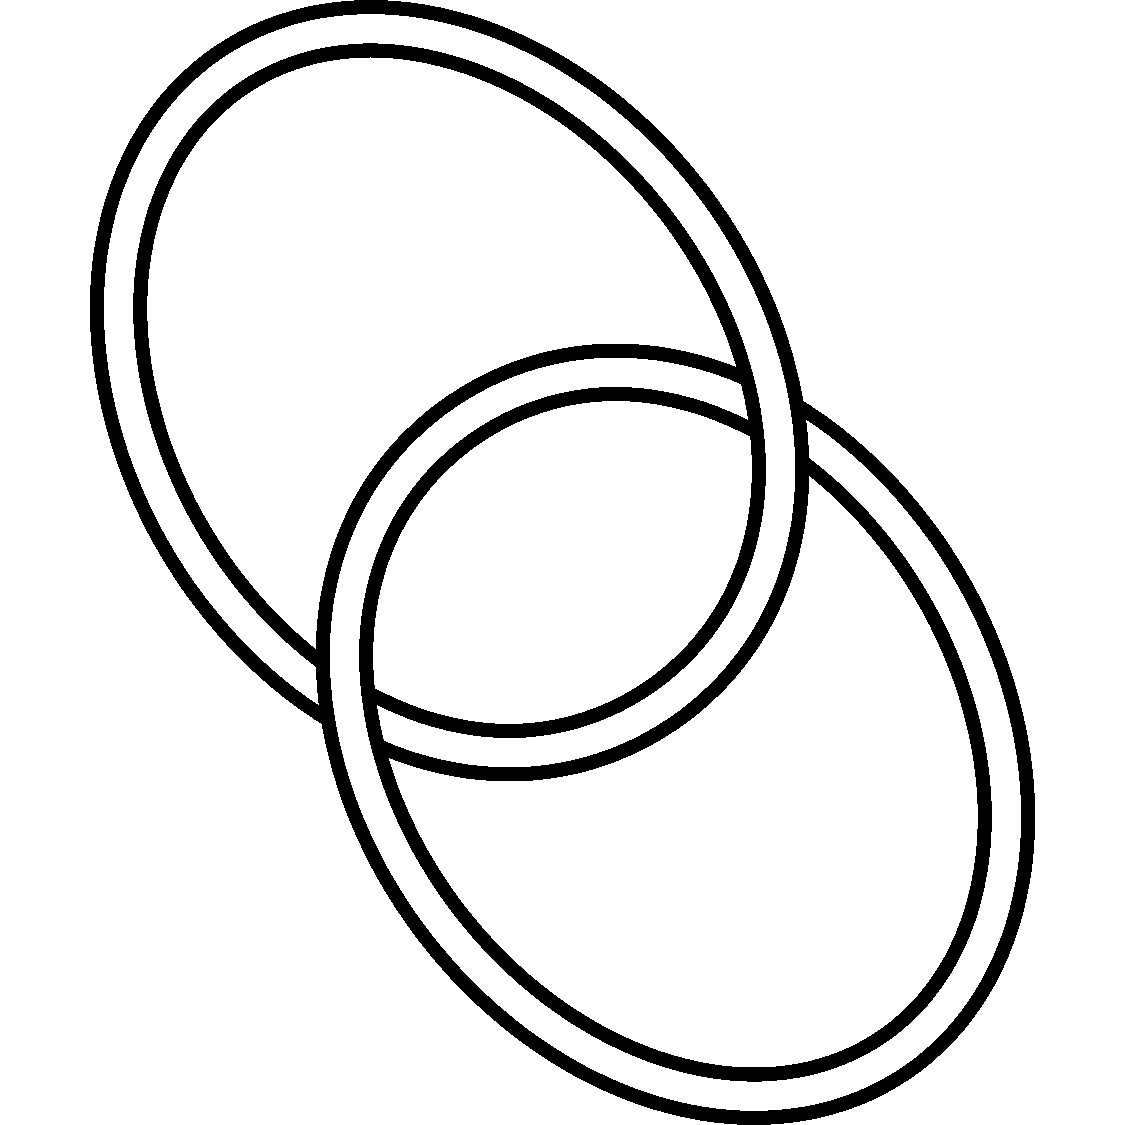
\includegraphics[scale=0.07,angle=0]{link2_1_2.pdf} 
& 
$
\displaystyle{%
q^{N-1} \Big(\frac{q^N-q^{-N}}{q-q^{-1}}\Big) + q^{2N} \Big(\frac{q^N-q^{-N}}{q-q^{-1}}\Big)^2 t^2 - q^{N+1} \Big(\frac{q^N-q^{-N}}{q-q^{-1}}\Big) t^2
}
$
\newline\newline\newline\newline
Checked up to $N=11$. Agrees with proposal of~\cite{gikv0705.1368}.
\\
\hline
%%%%%%%%%%%%%%%%%%%%%%%%%%%%%%%%%%%%%%%%%%%%%%%%%%%%
$3_{1}$ 
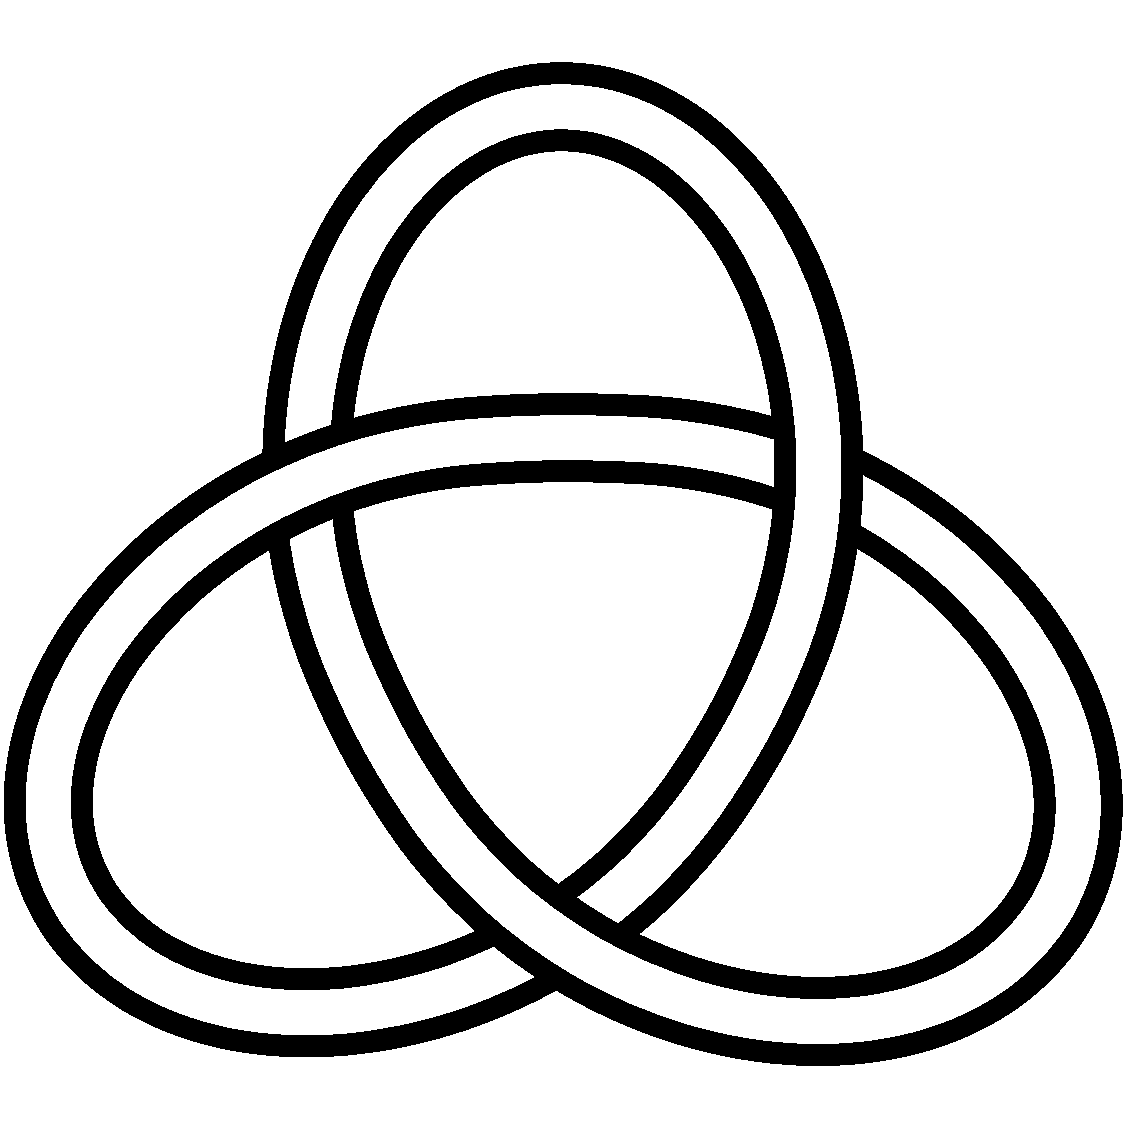
\includegraphics[scale=0.07,angle=0]{knot3_1.pdf} 
& 
$
\displaystyle{%
q^{2N-2} \Big( \frac{q^N-q^{-N}}{q-q^{-1}} + \frac{q^{N-1}-q^{-N+1}}{q-q^{-1}} q^{-1} (1 + q^{2N} t^{-1}) q^{4} t^{-2} \Big)
}
$
\newline\newline\newline\newline
Checked up to $N=11$. Extends result of~\cite{r0508510} to $N=3$ and $N=4$. 
\\
\hline
%%%%%%%%%%%%%%%%%%%%%%%%%%%%%%%%%%%%%%%%%%%%%%%%%%%%
$4_{1}$ 
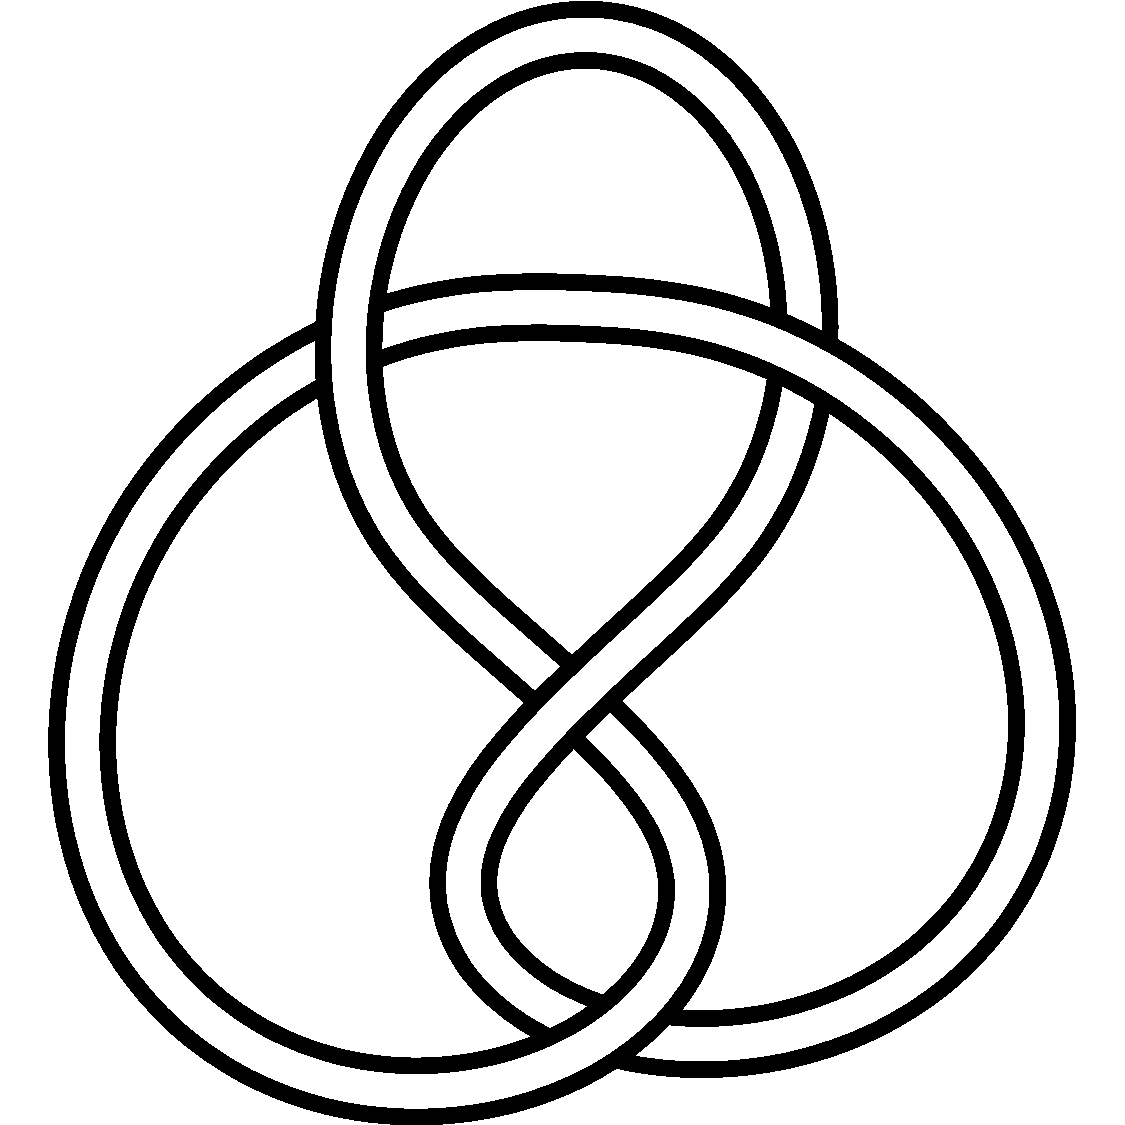
\includegraphics[scale=0.07,angle=0]{knot4_1.pdf} 
& 
$
\displaystyle{%
\frac{q^N-q^{-N}}{q-q^{-1}} + \frac{q^{N-1}-q^{-N+1}}{q-q^{-1}}  \Big( q^{2N+1} t^{-2} + q t^{-1} + q^{-1} t + q^{-2N-1} t^2 \Big)
}
$
\newline\newline\newline\newline
Checked up to $N=5$. Extends result of~\cite{r0508510} to $N=3$ and $N=4$. 
\\
\hline
%%%%%%%%%%%%%%%%%%%%%%%%%%%%%%%%%%%%%%%%%%%%%%%%%%%%
$4_{1}^2\,\text{{\tiny (v1)}}$ 
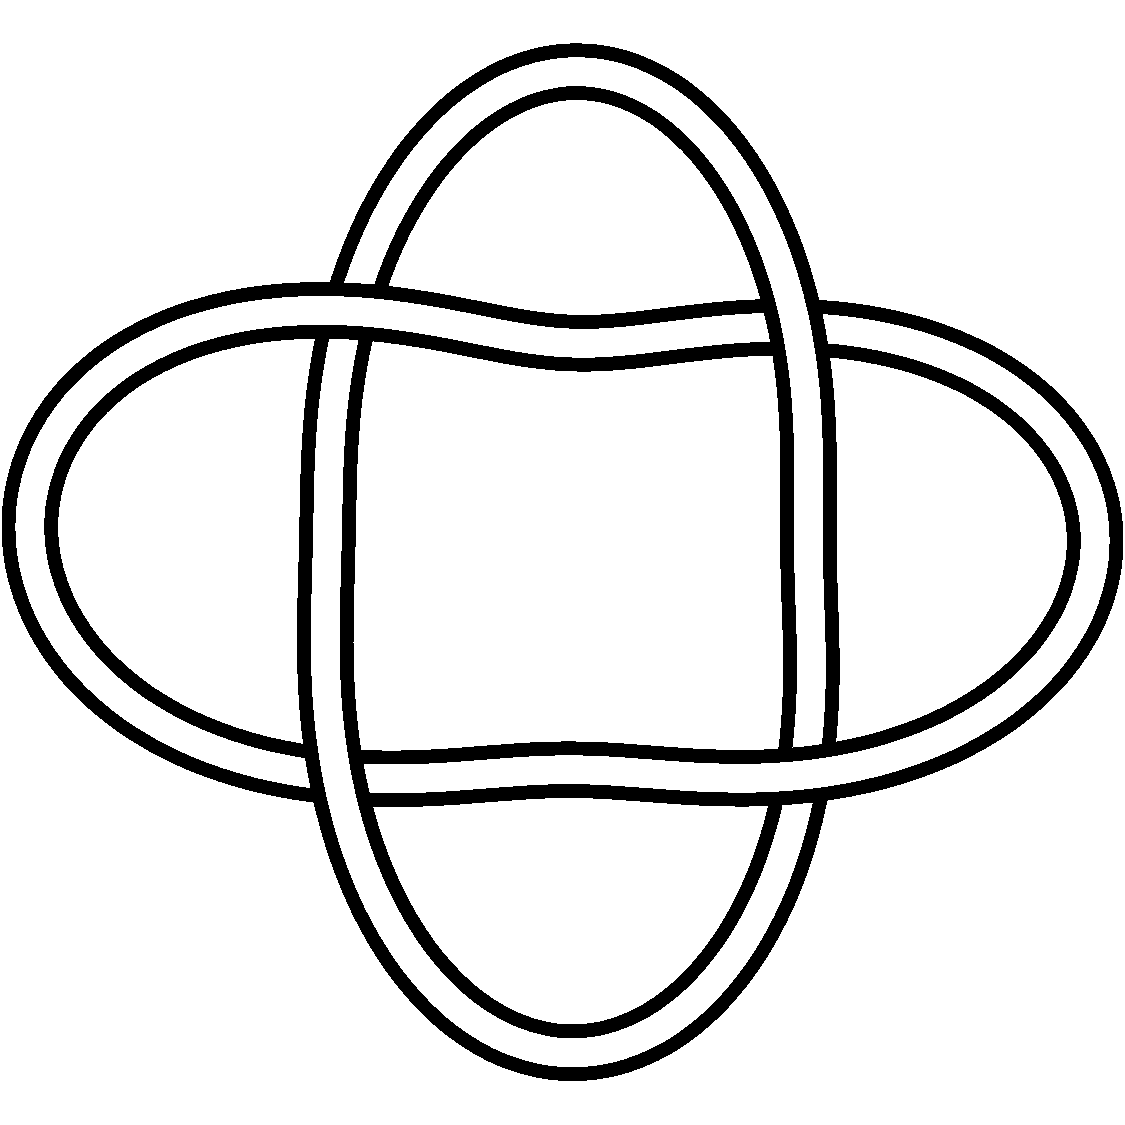
\includegraphics[scale=0.07,angle=0]{link4_1_2.pdf} 
& 
$
\displaystyle{%
\frac{q^{-4 N}}{\left(q^2 - 1\right)^2} \left(q^{2-2 N} \left(q^{2 N}-1\right)^2 t^4+\left(q^2 - 1\right) \left(-q^2 t^2+t^4+q^{4 N} \left(q^2+t\right)-q^{2 N} (1+t) \left(q^2+(t-1) t^2\right)\right)\right) 
}
$
\newline\newline\newline\newline
Checked up to $N=5$.
\\
\hline
%%%%%%%%%%%%%%%%%%%%%%%%%%%%%%%%%%%%%%%%%%%%%%%%%%%%
$4_{1}^2\,\text{{\tiny (v2)}}$ 
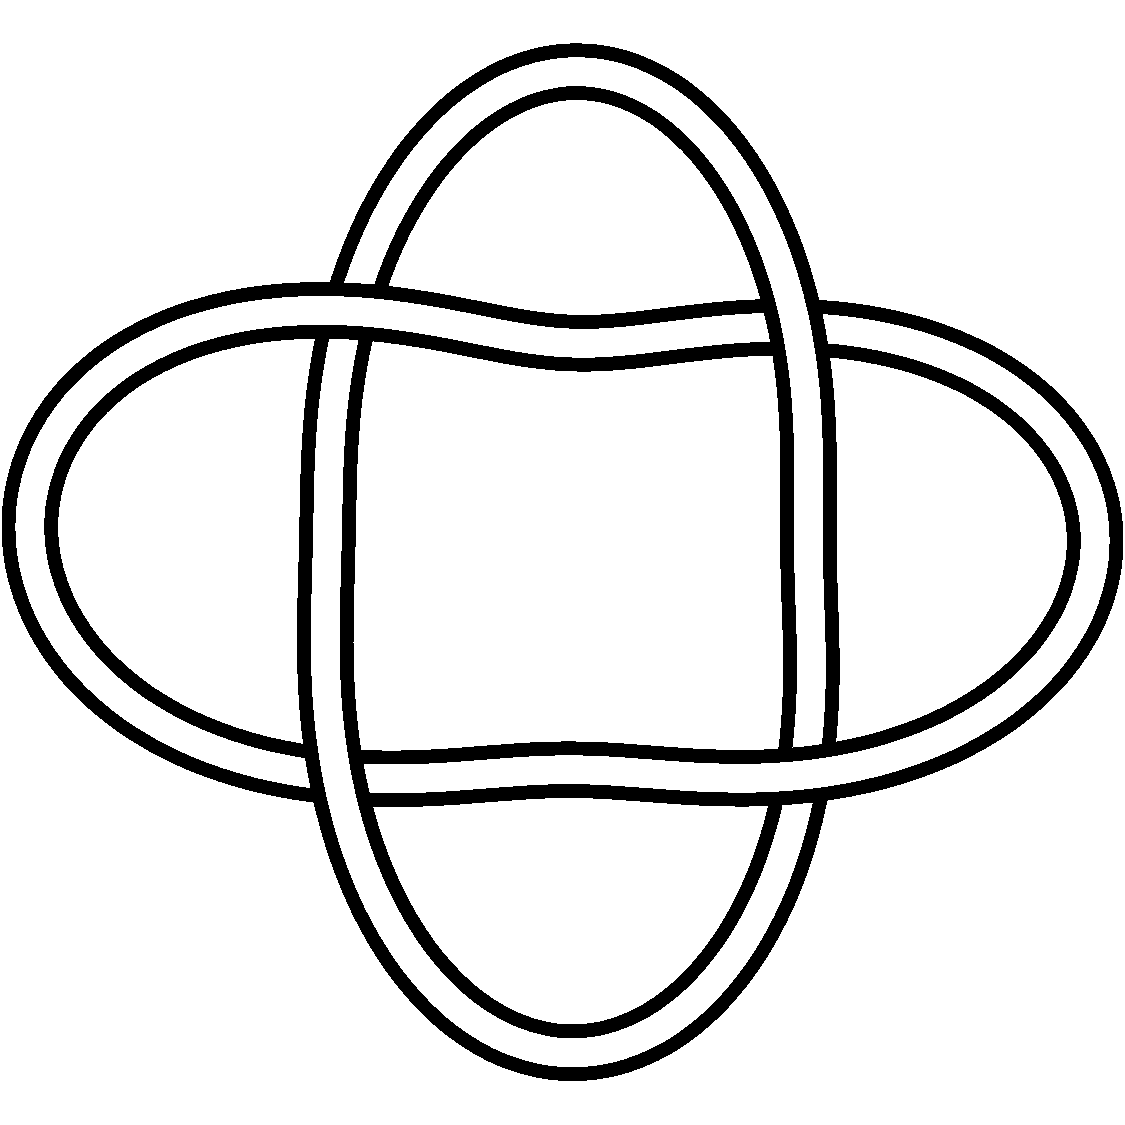
\includegraphics[scale=0.07,angle=0]{link4_1_2.pdf} 
& 
$
\displaystyle{%
\frac{q^{-2-6 N}}{\left(q^2-1\right)^2}} \left(q^2 t^3 \left(q^2-q^4+t\right)+q^{4 N} \left(q^6 \left(q^2-1\right)+q^2 \left(q^2-1\right) t^2+t^4\right) \right.
$
\newline
$
\displaystyle{%
\left. \qquad\qquad\quad -q^{2 N} \left(q^8+t^4-q^4 t^2 (1+t)+q^2 t^3 (1+t)+q^6 \left(t^2-1\right)\right)\right)
}
$
\newline\newline
Checked up to $N=5$.
\\
\hline
%%%%%%%%%%%%%%%%%%%%%%%%%%%%%%%%%%%%%%%%%%%%%%%%%%%%
$5_{1}$ 
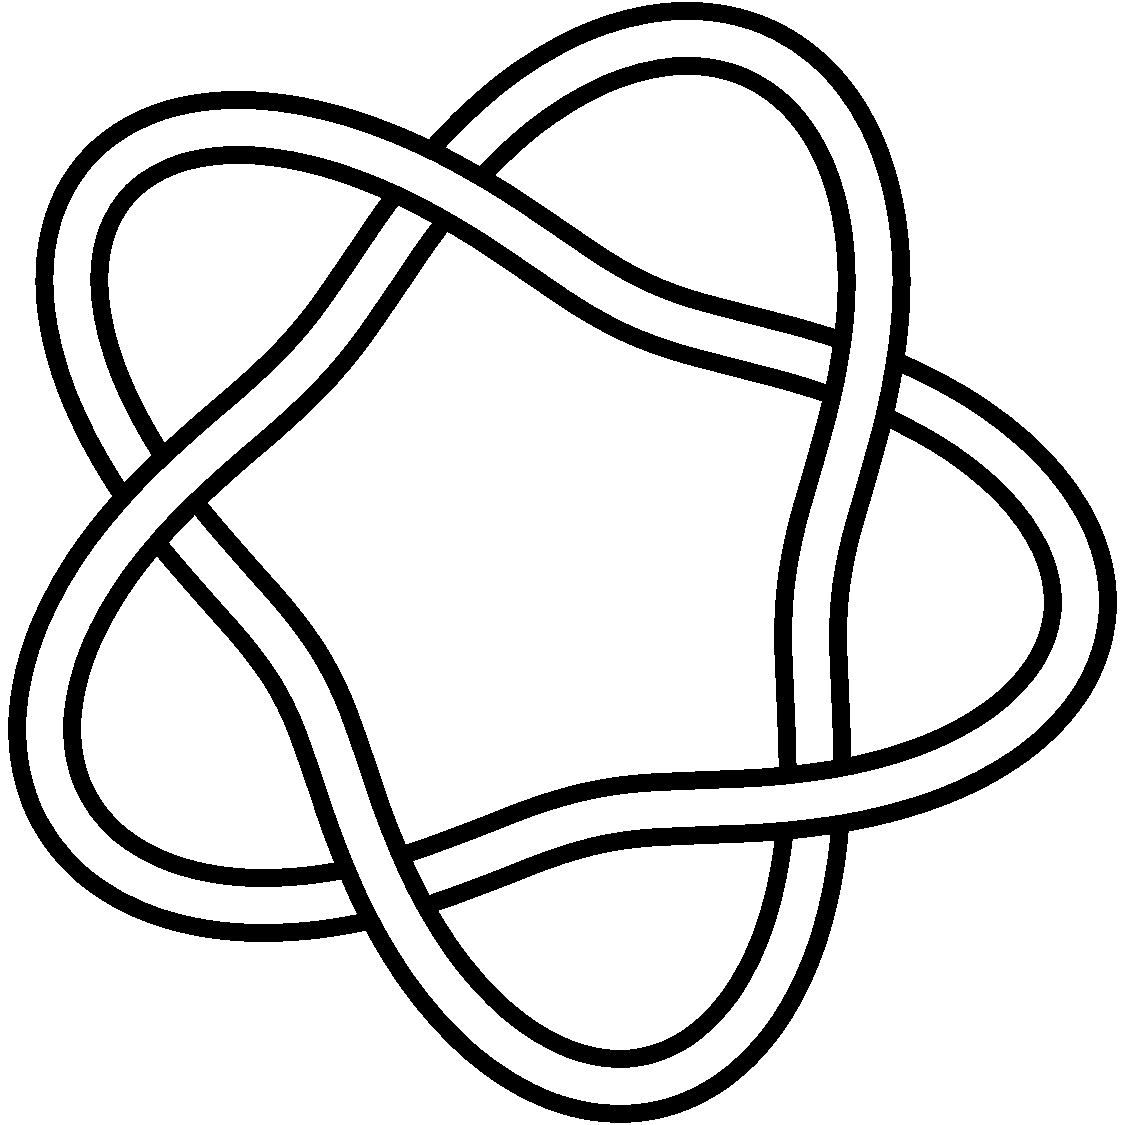
\includegraphics[scale=0.07,angle=0]{knot5_1.pdf} 
& 
$
\displaystyle{%
q^{4N-4} \Big( \frac{q^N-q^{-N}}{q-q^{-1}} + \frac{q^{N-1}-q^{-N+1}}{q-q^{-1}} q^{-1} (1 + q^{2N} t^{-1}) (q^{4} t^{-2} + q^{8} t^{-4}) \Big)
}
$
\newline\newline\newline\newline
Checked up to $N=6$. Extends result of~\cite{r0508510} to $N=3$ and $N=4$. 
\\
\hline
%%%%%%%%%%%%%%%%%%%%%%%%%%%%%%%%%%%%%%%%%%%%%%%%%%%%
$5_{2}$ 

\includegraphics[scale=0.07,angle=0]{knot5_2.pdf} 
& 
$
\displaystyle{%
\KR_{2} = \frac{1}{q^3}+\frac{1}{q}+\frac{t}{q^3}+\frac{t^2}{q^7}+\frac{t^2}{q^5}+\frac{t^3}{q^9}+\frac{t^4}{q^9}+\frac{t^5}{q^{13}}
}
$
\newline 
$
\displaystyle{%
\KR_{3} = \frac{1}{q^6}+\frac{1}{q^4}+\frac{1}{q^2}+\frac{t}{q^6}+\frac{t}{q^4}+\frac{t^2}{q^{12}}+\frac{t^2}{q^{10}}+\frac{t^2}{q^8}+\frac{t^2}{q^6}+\frac{t^3}{q^{14}}+\frac{t^3}{q^{12}}+\frac{t^4}{q^{14}}+\frac{t^4}{q^{12}}+\frac{t^5}{q^{20}}+\frac{t^5}{q^{18}}
}
$
\newline 
$
\displaystyle{%
\KR_{4} = \frac{1}{q^9}+\frac{1}{q^7}+\frac{1}{q^5}+\frac{1}{q^3}+\frac{t}{q^9}+\frac{t}{q^7}+\frac{t}{q^5}+\frac{t^2}{q^{17}}+\frac{t^2}{q^{15}}+\frac{t^2}{q^{13}}+\frac{t^2}{q^{11}}+\frac{t^2}{q^9}+\frac{t^2}{q^7}+\frac{t^3}{q^{19}}+\frac{t^3}{q^{17}}+\frac{t^3}{q^{15}}
}
$
\newline
$
\displaystyle{%
\qquad\qquad +\frac{t^4}{q^{19}}+\frac{t^4}{q^{17}}+\frac{t^4}{q^{15}}+\frac{t^5}{q^{27}}+\frac{t^5}{q^{25}}+\frac{t^5}{q^{23}}
}
$
\\
\hline
%%%%%%%%%%%%%%%%%%%%%%%%%%%%%%%%%%%%%%%%%%%%%%%%%%%%
$5_{1}^2\,\text{{\tiny (v1\&v2)}}$ 
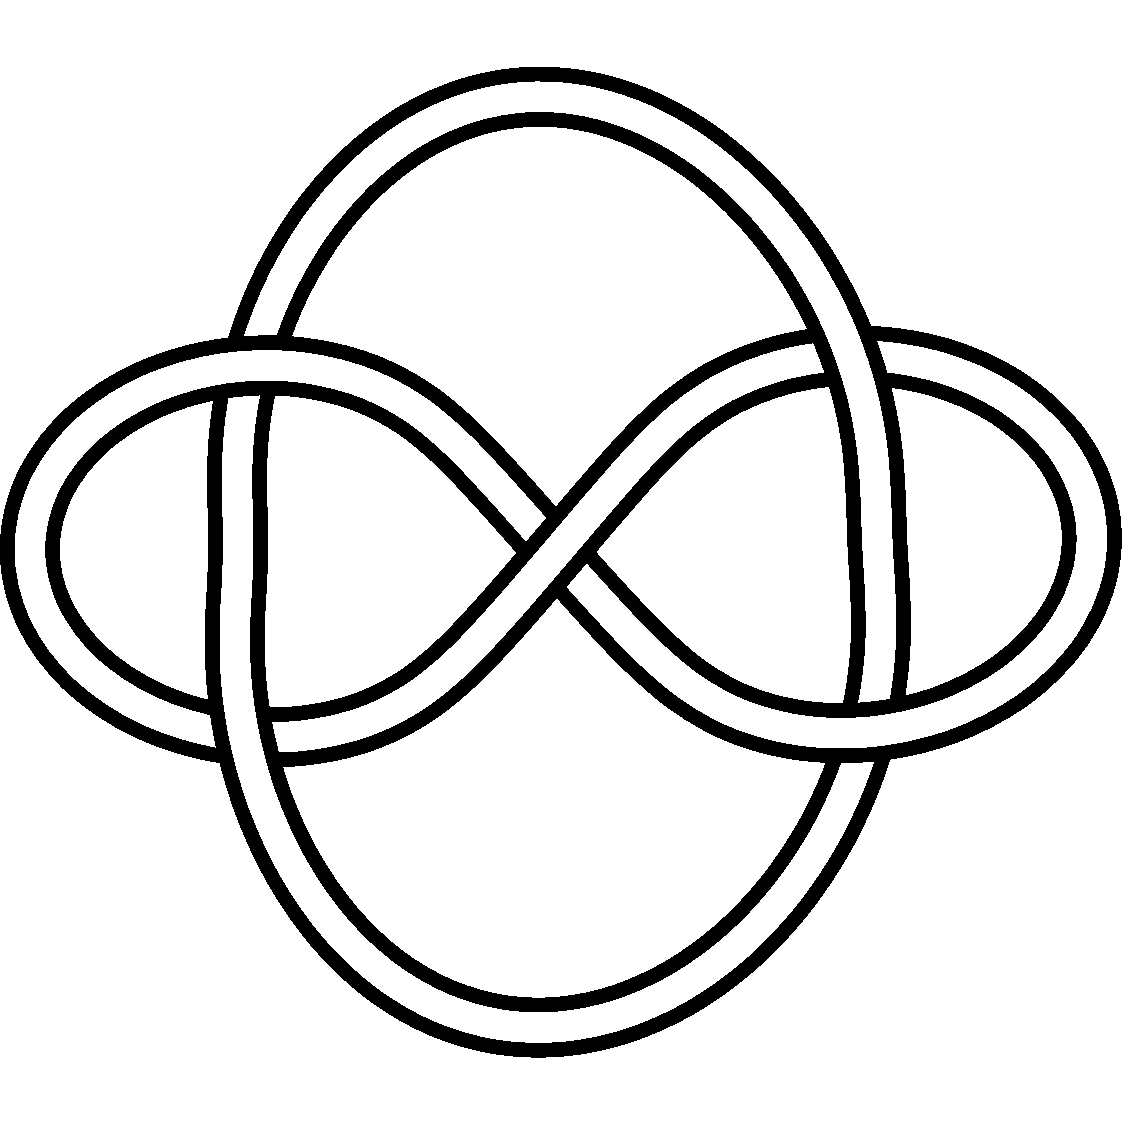
\includegraphics[scale=0.07,angle=0]{link5_1_2.pdf} 
& 
$
\displaystyle{%
\frac{q^{-2-4 N}}{\left(q^2-1\right)^2} \left(q^{4+2 N} \left(q^{2 N}-1\right)^2+t^{-2}\left(\left(q^2-1\right) \left(q^{2 N}-q^2\right) \left(q^{2+4 N} (q-t) (q+t)+t^4 \left(q^2+t\right) \right.\right.\right.
}
$
\newline
$
\displaystyle{%
\left.\left.\left. \qquad\qquad\quad+q^{2 N} t \left(q^2+t\right) \left(q^2+t^2\right)\right)\right)\right)
}
$
\newline\newline
Checked up to $N=4$.
\\
\hline
%%%%%%%%%%%%%%%%%%%%%%%%%%%%%%%%%%%%%%%%%%%%%%%%%%%%
$6_{1}$ 
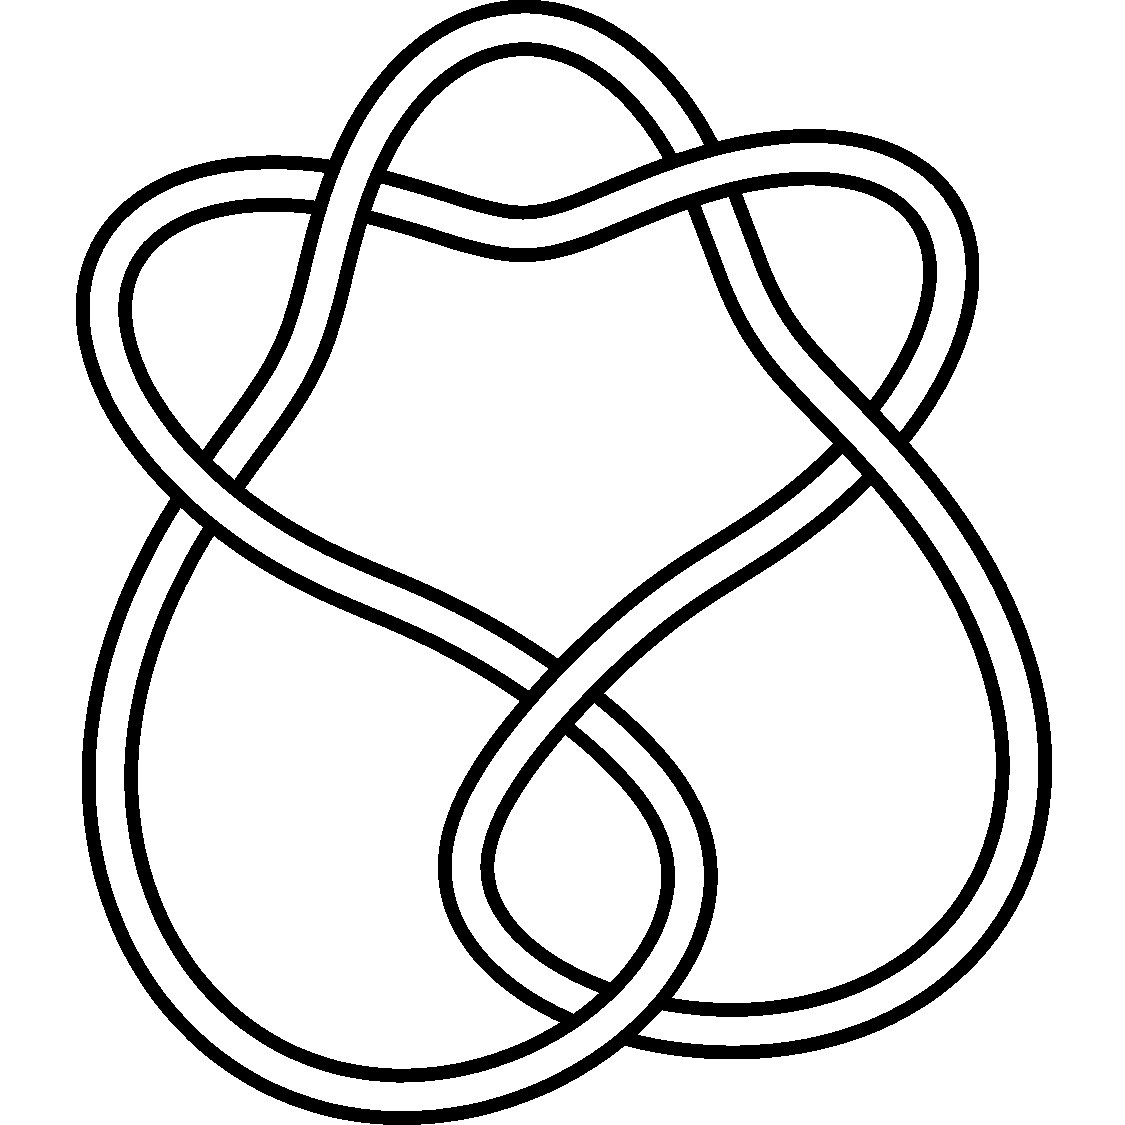
\includegraphics[scale=0.07,angle=0]{knot6_1.pdf} 
& 
$
\displaystyle{%
\KR_{2} = \frac{1}{q}+2 q+\frac{q^5}{t^2}+\frac{q}{t}+\frac{t}{q^3}+\frac{t}{q}+\frac{t^2}{q^5}+\frac{t^3}{q^5}+\frac{t^4}{q^9}
}
$
\newline 
$
\displaystyle{%
\KR_{3} = 2+\frac{1}{q^2}+2 q^2+\frac{q^6}{t^2}+\frac{q^8}{t^2}+\frac{1}{t}+\frac{q^2}{t}+t+\frac{t}{q^6}+\frac{t}{q^4}+\frac{t}{q^2}+\frac{t^2}{q^8}+\frac{t^2}{q^6}+\frac{t^3}{q^8}+\frac{t^3}{q^6}+\frac{t^4}{q^{14}}+\frac{t^4}{q^{12}}
}
$
\\
\hline
%%%%%%%%%%%%%%%%%%%%%%%%%%%%%%%%%%%%%%%%%%%%%%%%%%%%
$6_{2}$ 
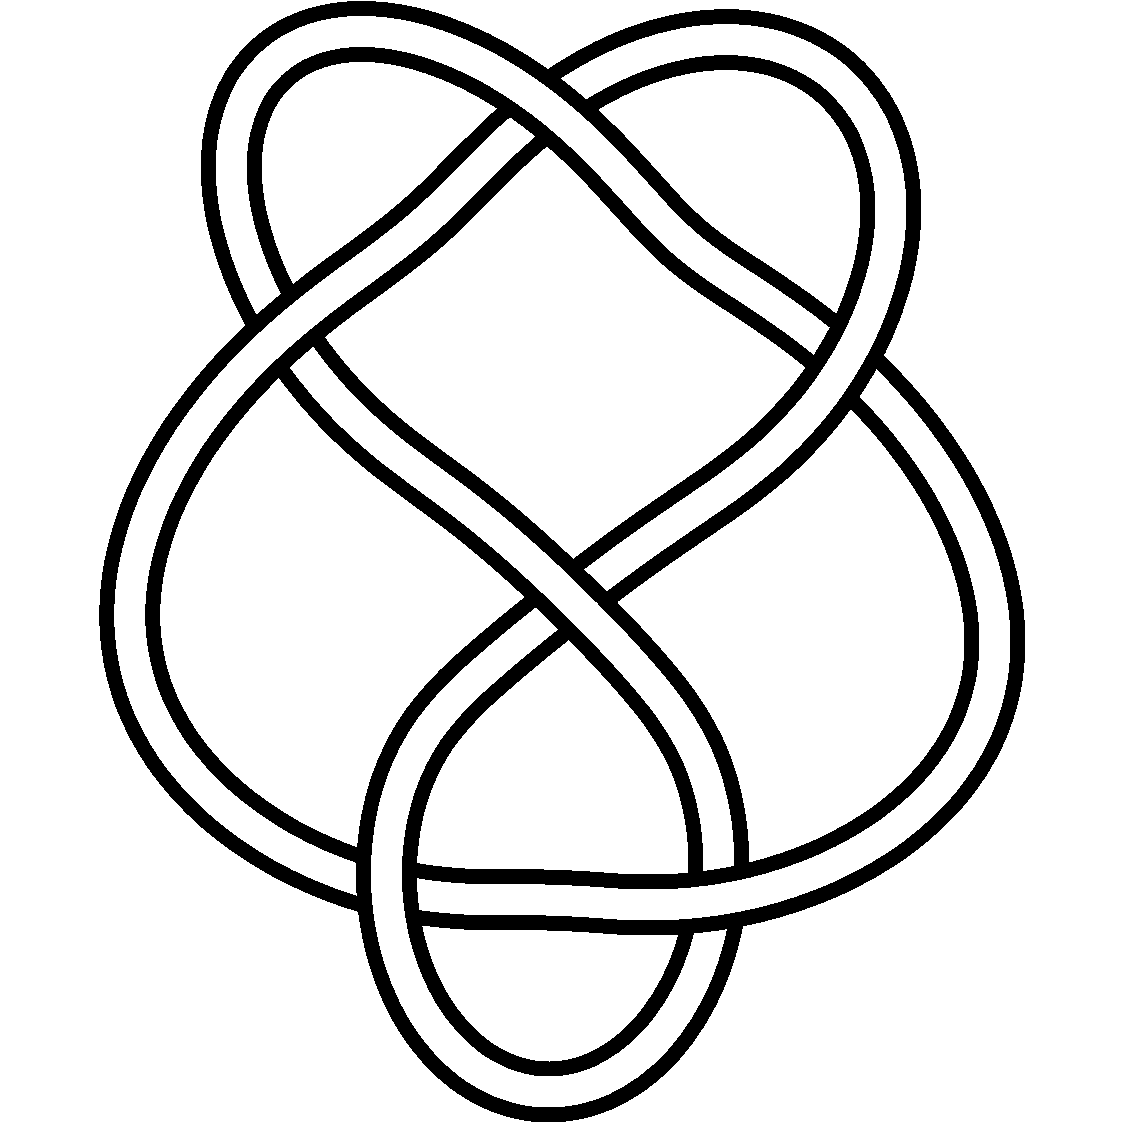
\includegraphics[scale=0.07,angle=0]{knot6_2.pdf} 
& 
$
\displaystyle{%
\KR_{2} = \frac{1}{q^3}+\frac{2}{q}+\frac{q^3}{t^2}+\frac{1}{q t}+\frac{t}{q^5}+\frac{t}{q^3}+\frac{t^2}{q^7}+\frac{t^2}{q^5}+\frac{t^3}{q^9}+\frac{t^3}{q^7}+\frac{t^4}{q^{11}}
}
$
\newline 
$
\displaystyle{%
\KR_{3} = 1+\frac{1}{q^6}+\frac{1}{q^4}+\frac{2}{q^2}+\frac{q^2}{t^2}+\frac{q^4}{t^2}+\frac{1}{q^4 t}+\frac{1}{q^2 t}+\frac{t}{q^8}+\frac{2 t}{q^6}+\frac{t}{q^4}+\frac{t^2}{q^{12}}+\frac{t^2}{q^{10}}+\frac{t^2}{q^8}+\frac{t^2}{q^6}+\frac{t^3}{q^{14}}+\frac{t^3}{q^{12}}
}
$
\newline
$
\displaystyle{%
\qquad\qquad +\frac{t^3}{q^{10}}+\frac{t^3}{q^8}+\frac{t^4}{q^{16}}+\frac{t^4}{q^{14}}
}
$
\\
\hline
%%%%%%%%%%%%%%%%%%%%%%%%%%%%%%%%%%%%%%%%%%%%%%%%%%%%
$6_{3}$ 

\includegraphics[scale=0.07,angle=0]{knot6_3.pdf} 
& 
$
\displaystyle{%
\KR_{2} = \frac{2}{q}+2 q+\frac{q^7}{t^3}+\frac{q^3}{t^2}+\frac{q^5}{t^2}+\frac{q}{t}+\frac{q^3}{t}+\frac{t}{q^3}+\frac{t}{q}+\frac{t^2}{q^5}+\frac{t^2}{q^3}+\frac{t^3}{q^7}
}
$
\newline 
$
\displaystyle{%
\KR_{3} = 3+\frac{2}{q^2}+2 q^2+\frac{q^8}{t^3}+\frac{q^{10}}{t^3}+\frac{q^2}{t^2}+\frac{q^4}{t^2}+\frac{q^6}{t^2}+\frac{q^8}{t^2}+\frac{1}{t}+\frac{q^2}{t}+\frac{q^4}{t}+\frac{q^6}{t}+t+\frac{t}{q^6}+\frac{t}{q^4}+\frac{t}{q^2}+\frac{t^2}{q^8}
}
$
\newline
$
\displaystyle{%
\qquad\qquad +\frac{t^2}{q^6}+\frac{t^2}{q^4}+\frac{t^2}{q^2}+\frac{t^3}{q^{10}}+\frac{t^3}{q^8}
}
$
\\
\hline
%%%%%%%%%%%%%%%%%%%%%%%%%%%%%%%%%%%%%%%%%%%%%%%%%%%%
$6_{1}^2\,\text{{\tiny (v1)}}$ 
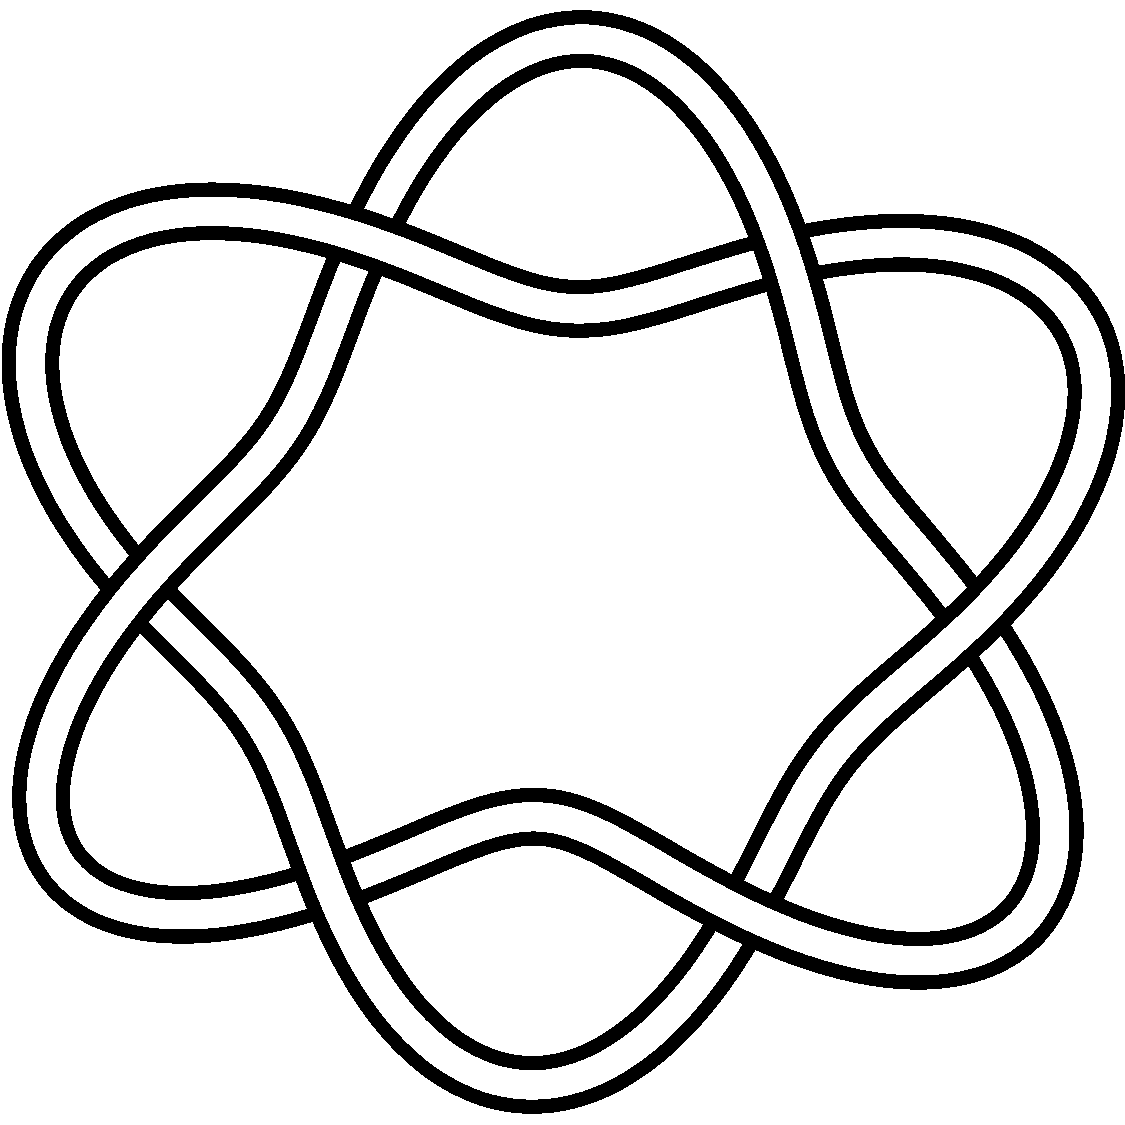
\includegraphics[scale=0.07,angle=0]{link6_1_2.pdf} 
& 
$
\displaystyle{%
\KR_{2} = \frac{1}{q^6}+\frac{1}{q^4}+\frac{t^2}{q^8}+\frac{t^3}{q^{12}}+\frac{t^4}{q^{12}}+\frac{t^5}{q^{16}}+\frac{t^6}{q^{18}}+\frac{t^6}{q^{16}}
}
$
\newline 
$
\displaystyle{%
\KR_{3} = \frac{1}{q^{12}}+\frac{1}{q^{10}}+\frac{1}{q^8}+\frac{t^2}{q^{14}}+\frac{t^2}{q^{12}}+\frac{t^3}{q^{20}}+\frac{t^3}{q^{18}}+\frac{t^4}{q^{18}}+\frac{t^4}{q^{16}}+\frac{t^5}{q^{24}}+\frac{t^5}{q^{22}}+\frac{t^6}{q^{26}}+\frac{2 t^6}{q^{24}}+\frac{2 t^6}{q^{22}}+\frac{t^6}{q^{20}}
}
$
\newline 
$
\displaystyle{%
\KR_{4} = \frac{1}{q^{18}}+\frac{1}{q^{16}}+\frac{1}{q^{14}}+\frac{1}{q^{12}}+\frac{t^2}{q^{20}}+\frac{t^2}{q^{18}}+\frac{t^2}{q^{16}}+\frac{t^3}{q^{28}}+\frac{t^3}{q^{26}}+\frac{t^3}{q^{24}}+\frac{t^4}{q^{24}}+\frac{t^4}{q^{22}}+\frac{t^4}{q^{20}}+\frac{t^5}{q^{32}}+\frac{t^5}{q^{30}}
}
$
\newline
$
\displaystyle{%
\qquad\qquad +\frac{t^5}{q^{28}}+\frac{t^6}{q^{34}}+\frac{2 t^6}{q^{32}}+\frac{3 t^6}{q^{30}}+\frac{3 t^6}{q^{28}}+\frac{2 t^6}{q^{26}}+\frac{t^6}{q^{24}}
}
$
\\
\hline
%%%%%%%%%%%%%%%%%%%%%%%%%%%%%%%%%%%%%%%%%%%%%%%%%%%%
$6_{1}^2\,\text{{\tiny (v2)}}$ 
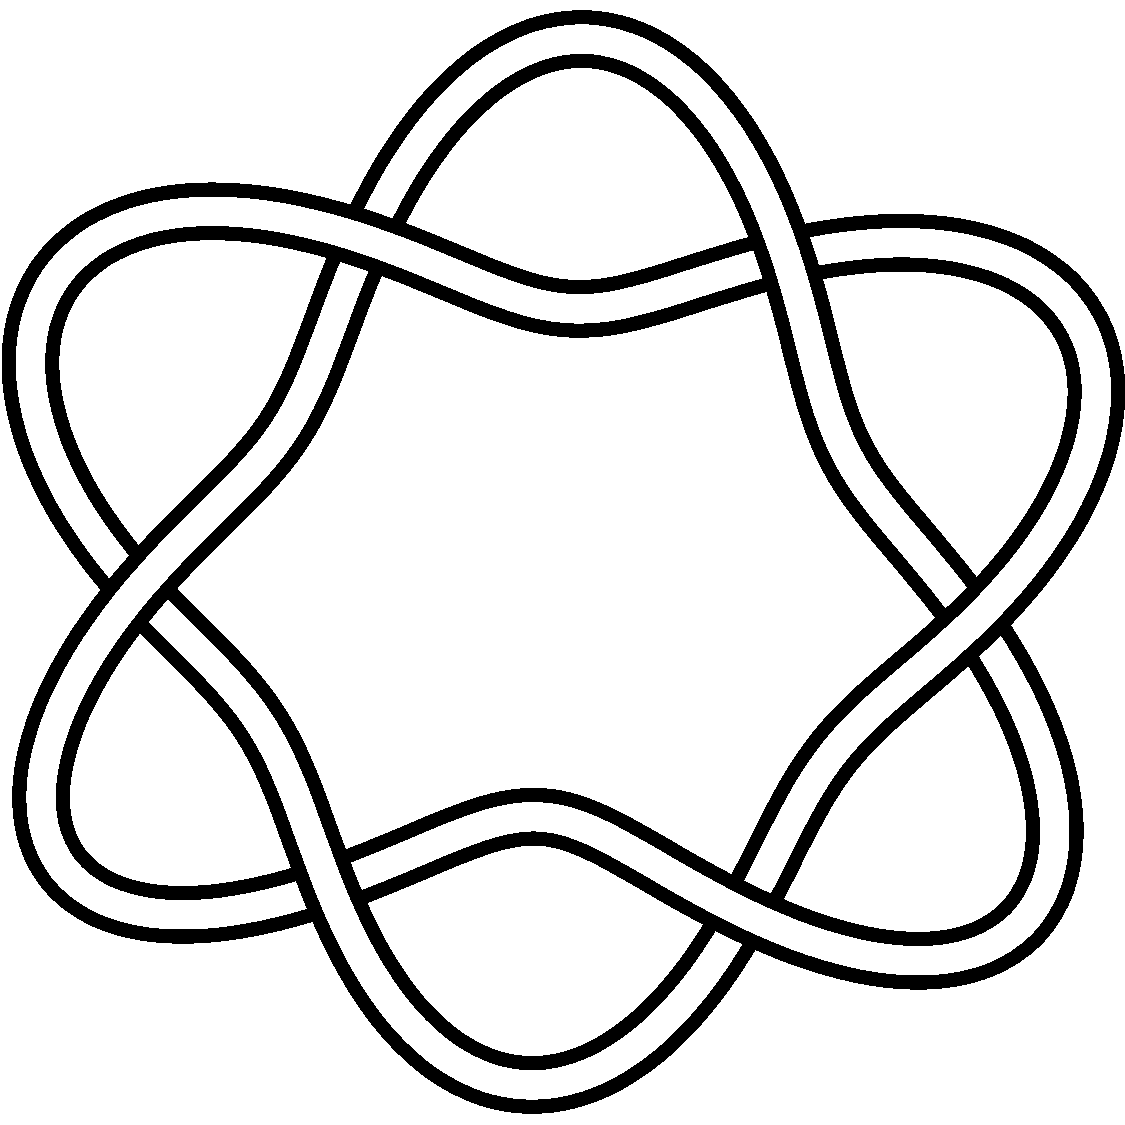
\includegraphics[scale=0.07,angle=0]{link6_1_2.pdf} 
& 
$
\displaystyle{%
\KR_{2} = 1+\frac{1}{q^2}+\frac{t^2}{q^6}+\frac{t^3}{q^6}+\frac{t^4}{q^{10}}+\frac{t^6}{q^{14}}+\frac{t^6}{q^{12}}+\frac{t q^{12}}{q^{14}}
}
$
\newline 
$
\displaystyle{%
\KR_{3} = TODO
}
$
\\
\hline
%%%%%%%%%%%%%%%%%%%%%%%%%%%%%%%%%%%%%%%%%%%%%%%%%%%%
$6_{1}^3\,\text{{\tiny (v1)}}$ 
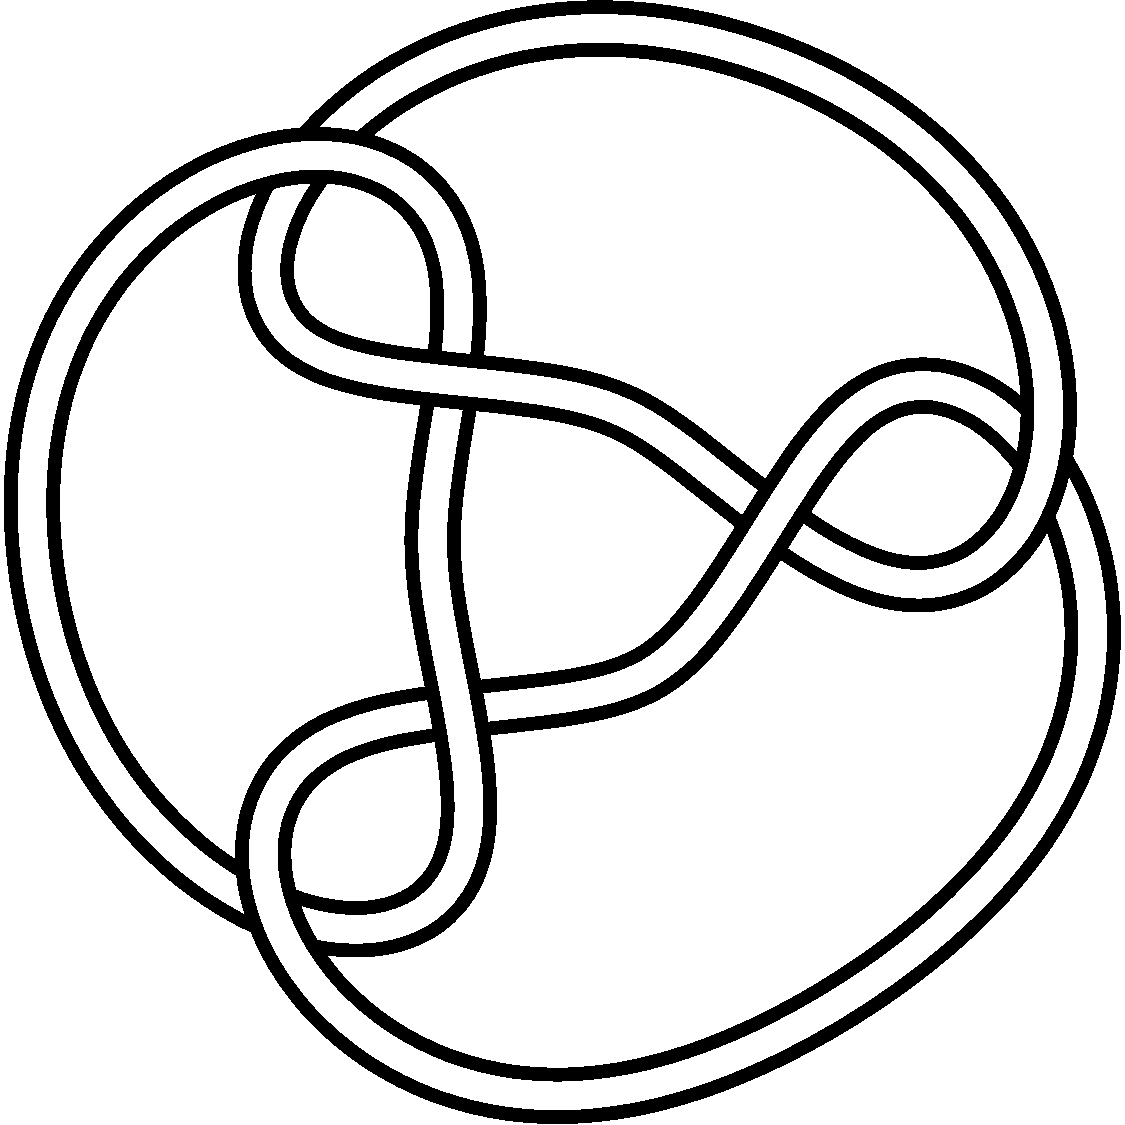
\includegraphics[scale=0.07,angle=0]{link6_1_3.pdf} 
& 
$
\displaystyle{%
\KR_{2} = \frac{1}{q^3}+\frac{1}{q}+\frac{2 t}{q^3}+\frac{2 t^2}{q^7}+\frac{t^2}{q^5}+\frac{t^3}{q^9}+\frac{3 t^4}{q^{11}}+\frac{3 t^4}{q^9}+\frac{t^5}{q^{11}}+\frac{t^6}{q^{15}}
}
$
\newline 
$
\displaystyle{%
\KR_{3} = \frac{1}{q^6}+\frac{1}{q^4}+\frac{1}{q^2}+\frac{2 t}{q^6}+\frac{2 t}{q^4}+\frac{2 t^2}{q^{12}}+\frac{2 t^2}{q^{10}}+\frac{t^2}{q^8}+\frac{t^2}{q^6}+\frac{t^3}{q^{14}}+\frac{t^3}{q^{12}}+\frac{3 t^4}{q^{18}}+\frac{6 t^4}{q^{16}}+\frac{6 t^4}{q^{14}}+\frac{3 t^4}{q^{12}}+\frac{t^5}{q^{16}}
}
$
\newline
$
\displaystyle{%
\qquad\qquad +\frac{t^5}{q^{14}}+\frac{t^6}{q^{24}}+\frac{3 t^6}{q^{22}}+\frac{3 t^6}{q^{20}}+\frac{t^6}{q^{18}}
}
$
\\
\hline
%%%%%%%%%%%%%%%%%%%%%%%%%%%%%%%%%%%%%%%%%%%%%%%%%%%%
$6_{1}^3\,\text{{\tiny (v2)}}$ 
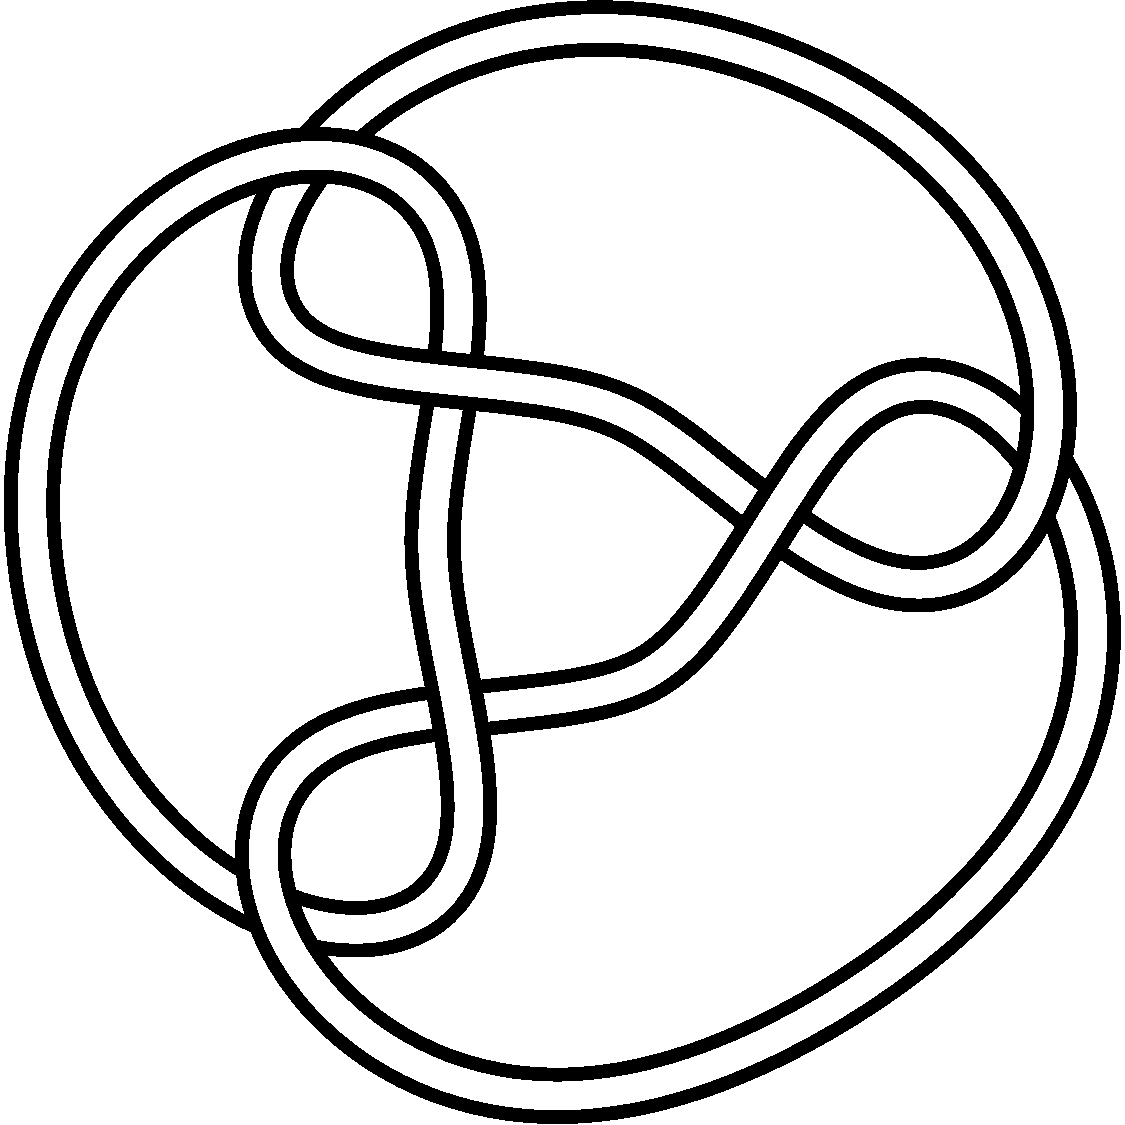
\includegraphics[scale=0.07,angle=0]{link6_1_3.pdf} 
& 
$
\displaystyle{%
\KR_{2} = \frac{1}{q^3}+\frac{1}{q}+\frac{2 t}{q^3}+\frac{2 t^2}{q^7}+\frac{t^2}{q^5}+\frac{t^3}{q^9}+\frac{3 t^4}{q^{11}}+\frac{3 t^4}{q^9}+\frac{t^5}{q^{11}}+\frac{t^6}{q^{15}}
}
$
\newline 
$
\displaystyle{%
\KR_{3} = 2+5 q^2+5 q^4+3 q^6+\frac{q^{10}}{t^4}+\frac{2 q^{12}}{t^4}+\frac{2 q^{14}}{t^4}+\frac{q^{16}}{t^4}+\frac{2 q^{12}}{t^3}+\frac{2 q^{14}}{t^3}+\frac{q^4}{t^2}+\frac{4 q^6}{t^2}+\frac{4 q^8}{t^2}+\frac{2 q^{10}}{t^2}+\frac{q^{12}}{t^2}
}
$
\newline
$
\displaystyle{%
\qquad\qquad +\frac{q^4}{t}+\frac{q^6}{t}+q^2 t+q^4 t+\frac{t^2}{q^4}+\frac{t^2}{q^2}
}
$
\\
\hline
%%%%%%%%%%%%%%%%%%%%%%%%%%%%%%%%%%%%%%%%%%%%%%%%%%%%
$6_{2}^2\,\text{{\tiny (v1)}}$ 
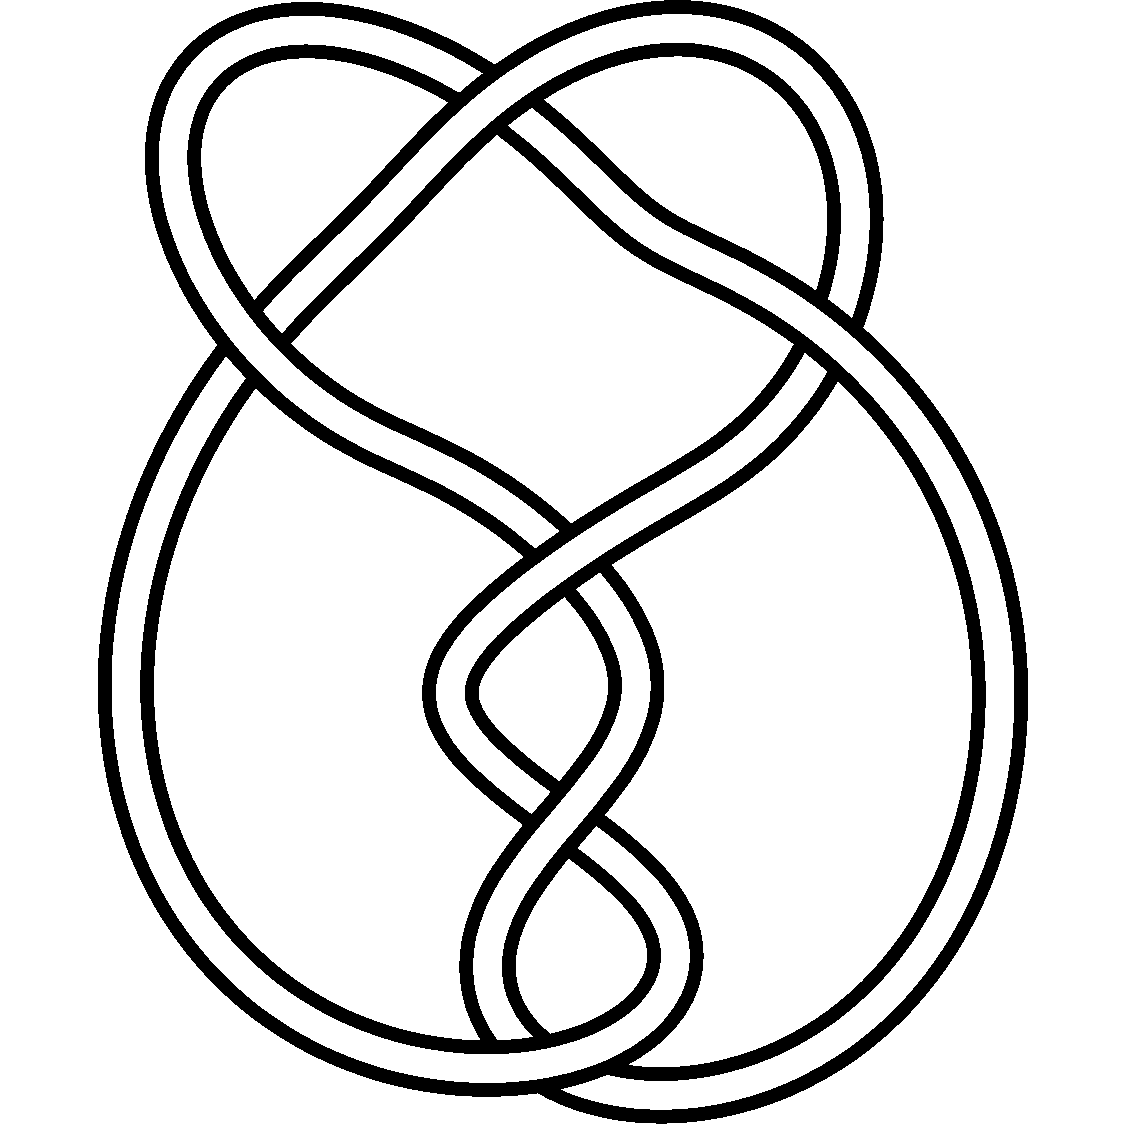
\includegraphics[scale=0.07,angle=0]{link6_2_2.pdf} 
& 
$
\displaystyle{%
\KR_{2} = \frac{1}{q^4}+\frac{1}{q^2}+\frac{t}{q^4}+\frac{t^2}{q^8}+\frac{t^2}{q^6}+\frac{t^3}{q^{10}}+\frac{t^3}{q^8}+\frac{t^4}{q^{12}}+\frac{t^4}{q^{10}}+\frac{t^5}{q^{14}}+\frac{t^6}{q^{16}}+\frac{t^6}{q^{14}}
}
$
\newline 
$
\displaystyle{%
\KR_{3} = \frac{1}{q^8}+\frac{1}{q^6}+\frac{1}{q^4}+\frac{t}{q^8}+\frac{t}{q^6}+\frac{t^2}{q^{14}}+\frac{t^2}{q^{12}}+\frac{t^2}{q^{10}}+\frac{t^2}{q^8}+\frac{t^3}{q^{16}}+\frac{t^3}{q^{14}}+\frac{t^3}{q^{12}}+\frac{t^3}{q^{10}}+\frac{t^4}{q^{18}}+\frac{2 t^4}{q^{16}}+\frac{t^4}{q^{14}}
}
$
\newline
$
\displaystyle{%
\qquad\qquad +\frac{t^5}{q^{22}}+\frac{t^5}{q^{20}}+\frac{t^6}{q^{24}}+\frac{2 t^6}{q^{22}}+\frac{2 t^6}{q^{20}}+\frac{t^6}{q^{18}}
}
$
\\
\hline
%%%%%%%%%%%%%%%%%%%%%%%%%%%%%%%%%%%%%%%%%%%%%%%%%%%%
$6_{2}^2\,\text{{\tiny (v2)}}$ 
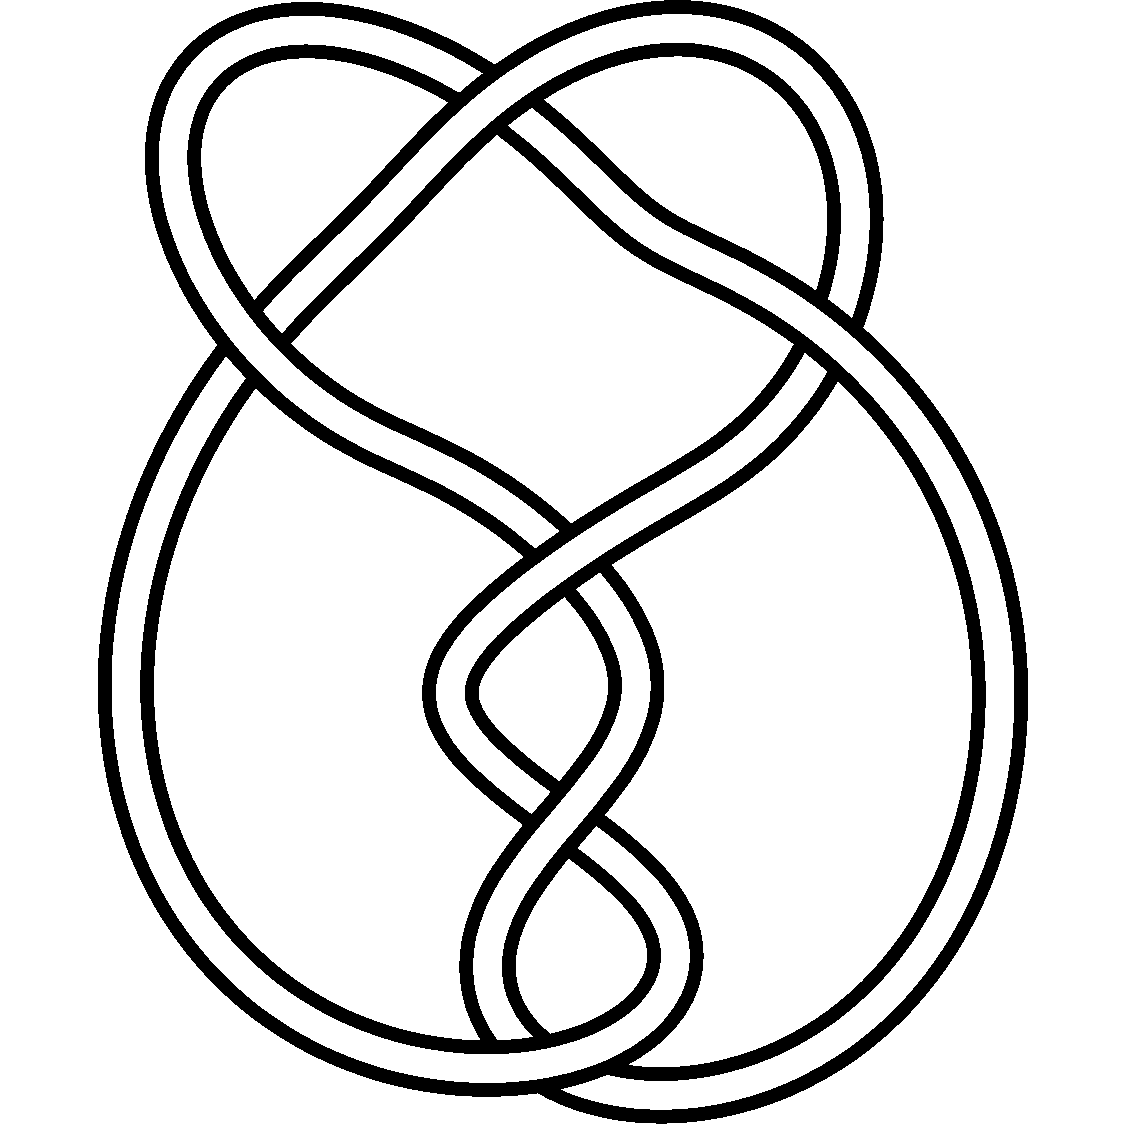
\includegraphics[scale=0.07,angle=0]{link6_2_2.pdf} 
& 
$
\displaystyle{%
\KR_{2} = q^2+q^4+\frac{q^{14}}{t^6}+\frac{q^{16}}{t^6}+\frac{q^{14}}{t^5}+\frac{q^{10}}{t^4}+\frac{q^{12}}{t^4}+\frac{q^8}{t^3}+\frac{q^{10}}{t^3}+\frac{q^6}{t^2}+\frac{q^8}{t^2}+\frac{q^4}{t}
}
$
\newline 
$
\displaystyle{%
\KR_{3} = q^4+q^6+q^8+\frac{q^{18}}{t^6}+\frac{2 q^{20}}{t^6}+\frac{2 q^{22}}{t^6}+\frac{q^{24}}{t^6}+\frac{q^{20}}{t^5}+\frac{q^{22}}{t^5}+\frac{q^{14}}{t^4}+\frac{2 q^{16}}{t^4}+\frac{q^{18}}{t^4}+\frac{q^{10}}{t^3}+\frac{q^{12}}{t^3}+\frac{q^{14}}{t^3}
}
$
\newline
$
\displaystyle{%
\qquad\qquad +\frac{q^{16}}{t^3}+\frac{q^8}{t^2}+\frac{q^{10}}{t^2}+\frac{q^{12}}{t^2}+\frac{q^{14}}{t^2}+\frac{q^6}{t}+\frac{q^8}{t}
}
$
\\
\hline
%%%%%%%%%%%%%%%%%%%%%%%%%%%%%%%%%%%%%%%%%%%%%%%%%%%%
$6_{2}^3\,\text{{\tiny (v1)}}$ 
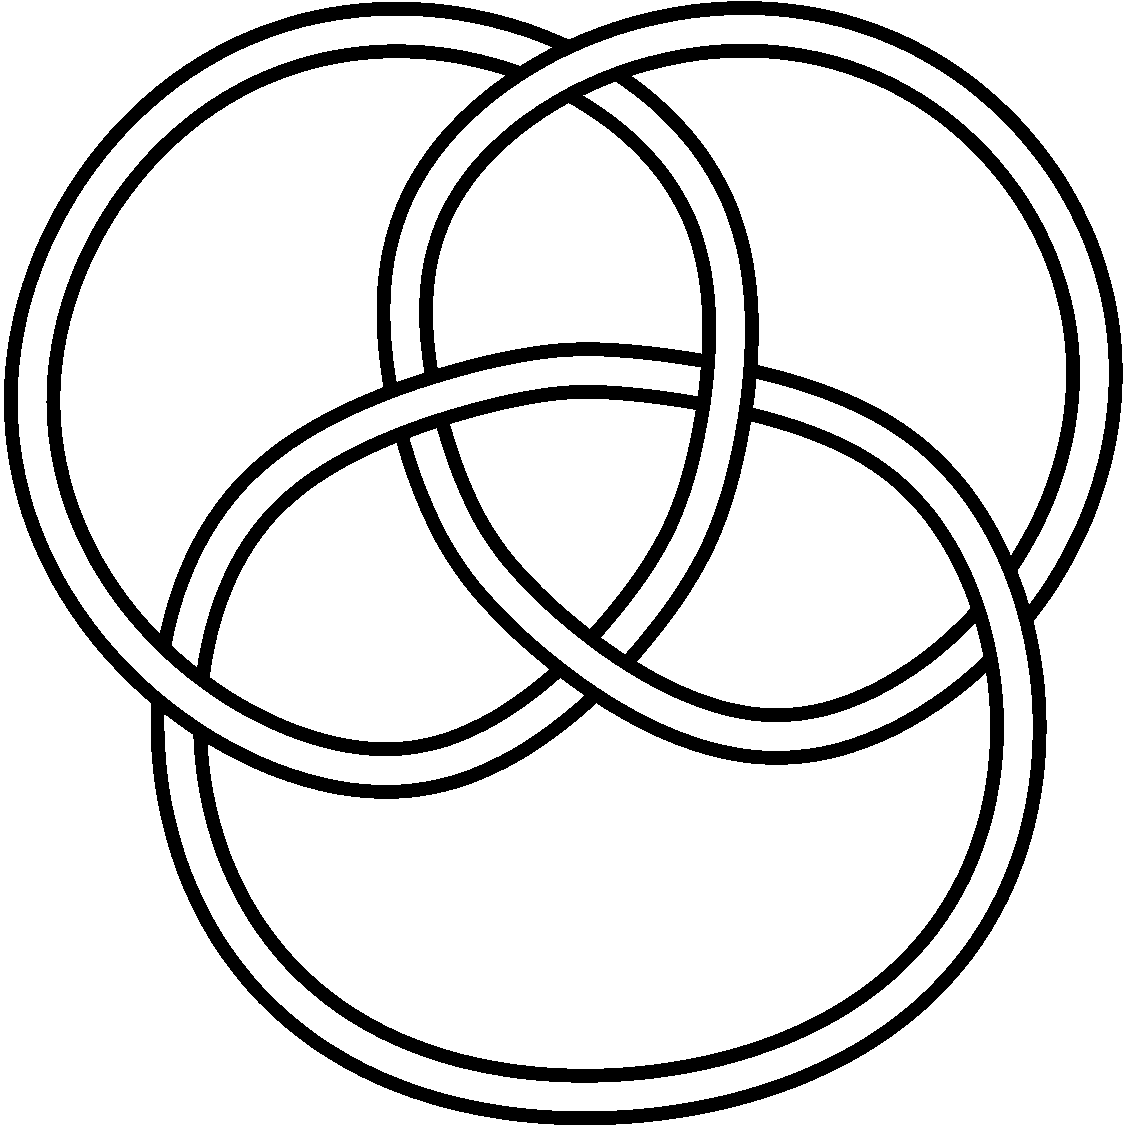
\includegraphics[scale=0.07,angle=0]{link6_2_3.pdf} 
& 
$
\displaystyle{%
\KR_{2} = \frac{2}{q}+2 q+\frac{q^3}{t^2}+\frac{q^5}{t^2}+\frac{t^2}{q^5}+\frac{t^2}{q^3}
}
$
\newline 
$
\displaystyle{%
\KR_{3} = 5+\frac{1}{q^4}+\frac{4}{q^2}+4 q^2+q^4+\frac{q^2}{t^2}+\frac{2 q^4}{t^2}+\frac{2 q^6}{t^2}+\frac{q^8}{t^2}+\frac{t^2}{q^8}+\frac{2 t^2}{q^6}+\frac{2 t^2}{q^4}+\frac{t^2}{q^2}
}
$
\\
\hline
%%%%%%%%%%%%%%%%%%%%%%%%%%%%%%%%%%%%%%%%%%%%%%%%%%%%
$6_{2}^3\,\text{{\tiny (v2)}}$ 
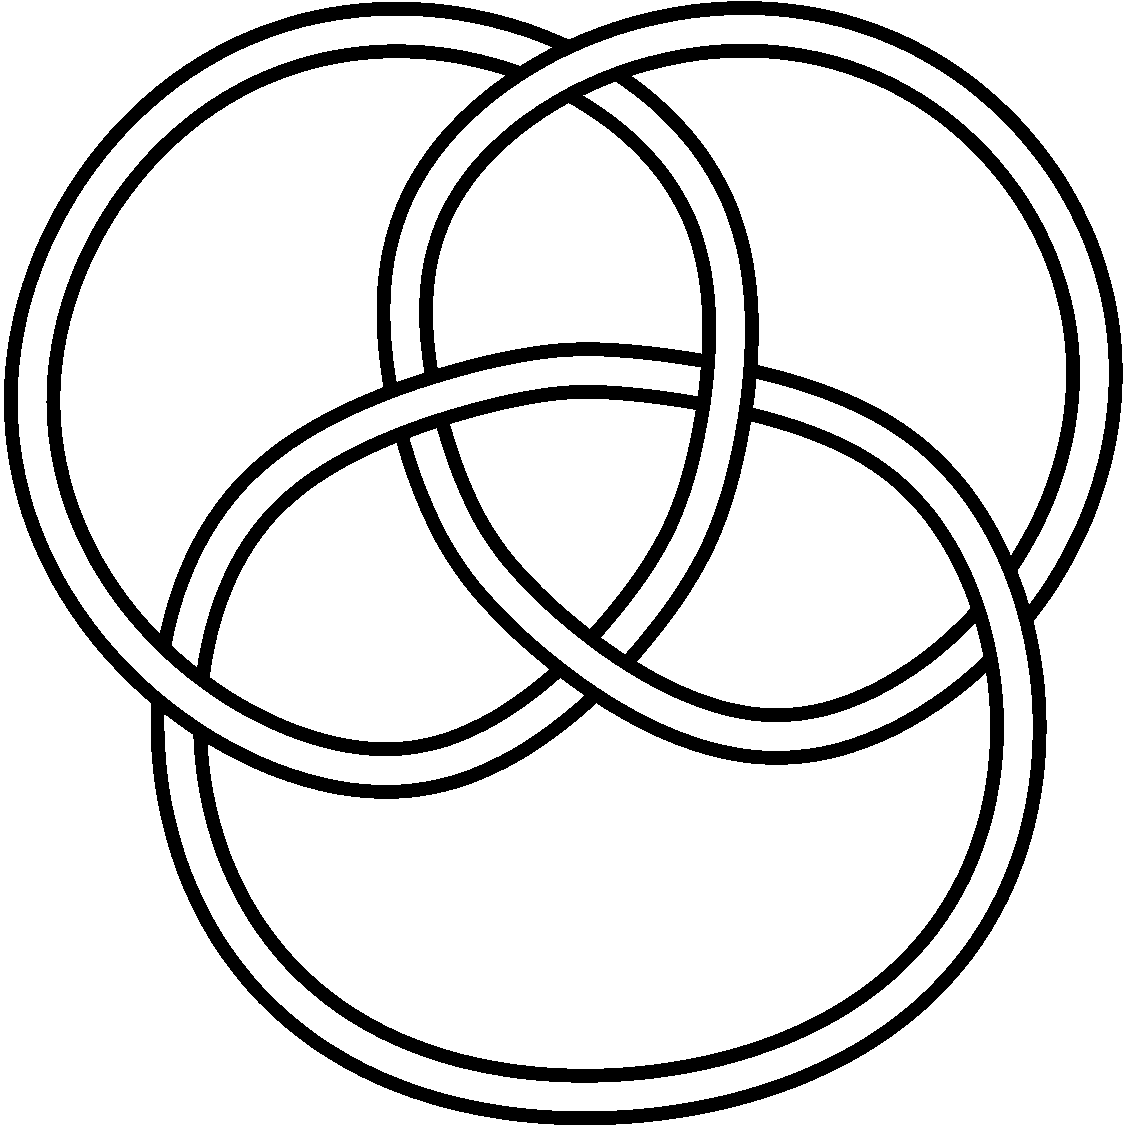
\includegraphics[scale=0.07,angle=0]{link6_2_3.pdf} 
& 
$
\displaystyle{%
\KR_{2} = \frac{4}{q}+4 q+\frac{q^7}{t^3}+\frac{q^3}{t^2}+\frac{2 q^5}{t^2}+\frac{2 q}{t}+\frac{2 t}{q}+\frac{2 t^2}{q^5}+\frac{t^2}{q^3}+\frac{t^3}{q^7}
}
$
\newline 
$
\displaystyle{%
\KR_{3} = 9+\frac{2}{q^4}+\frac{7}{q^2}+7 q^2+2 q^4+\frac{q^8}{t^3}+\frac{q^{10}}{t^3}+\frac{q^2}{t^2}+\frac{q^4}{t^2}+\frac{2 q^6}{t^2}+\frac{2 q^8}{t^2}+\frac{2}{t}+\frac{2 q^2}{t}+2 t+\frac{2 t}{q^2}+\frac{2 t^2}{q^8}+\frac{2 t^2}{q^6}
}
$
\newline
$
\displaystyle{%
\qquad\qquad +\frac{t^2}{q^4}+\frac{t^2}{q^2}+\frac{t^3}{q^{10}}+\frac{t^3}{q^8}
}
$
\\
\hline
%%%%%%%%%%%%%%%%%%%%%%%%%%%%%%%%%%%%%%%%%%%%%%%%%%%%
$6_{3}^2\,\text{{\tiny (v1)}}$ 

\includegraphics[scale=0.07,angle=0]{link6_3_2.pdf} 
& 
$
\displaystyle{%
\frac{q^{-2-6 N}}{\left(q^2-1\right)^2} \left(q^2 t^3 \left(q^2-q^4+t\right)+q^{4 N} \left(q^6 \left(q^2-1\right)+q^2 \left(q^2-1\right) t^2+t^4\right) \right.
}
$
\newline
$
\displaystyle{%
\left. \qquad\qquad\quad -q^{2 N} \left(q^8+t^4-q^4 t^2 (1+t)+q^2 t^3 (1+t)+q^6 \left(t^2-1\right)\right)\right)
}
$
\newline\newline
Checked up to $N=3$.
\\
\hline
%%%%%%%%%%%%%%%%%%%%%%%%%%%%%%%%%%%%%%%%%%%%%%%%%%%%
$6_{3}^2\,\text{{\tiny (v2)}}$ 

\includegraphics[scale=0.07,angle=0]{link6_3_2.pdf} 
& 
$
\displaystyle{%
\KR_{2} = q^2+q^4+\frac{q^{16}}{t^6}+\frac{q^{12}}{t^5}+\frac{q^{14}}{t^5}+\frac{2 q^{10}}{t^4}+\frac{q^{12}}{t^4}+\frac{2 q^{10}}{t^3}+\frac{2 q^6}{t^2}+\frac{q^8}{t^2}+\frac{q^4}{t}
}
$
\newline 
$
\displaystyle{%
\KR_{3} = q^4+q^6+q^8+\frac{q^{22}}{t^6}+\frac{q^{24}}{t^6}+\frac{q^{16}}{t^5}+\frac{q^{18}}{t^5}+\frac{q^{20}}{t^5}+\frac{q^{22}}{t^5}+\frac{q^{12}}{t^4}+\frac{3 q^{14}}{t^4}+\frac{3 q^{16}}{t^4}+\frac{q^{18}}{t^4}+\frac{2 q^{14}}{t^3}+\frac{2 q^{16}}{t^3}
}
$
\newline
$
\displaystyle{%
\qquad\qquad +\frac{2 q^8}{t^2}+\frac{2 q^{10}}{t^2}+\frac{q^{12}}{t^2}+\frac{q^{14}}{t^2}+\frac{q^6}{t}+\frac{q^8}{t}
}
$
\\
\hline
%%%%%%%%%%%%%%%%%%%%%%%%%%%%%%%%%%%%%%%%%%%%%%%%%%%%
$6_{3}^3\,\text{{\tiny (v1)}}$
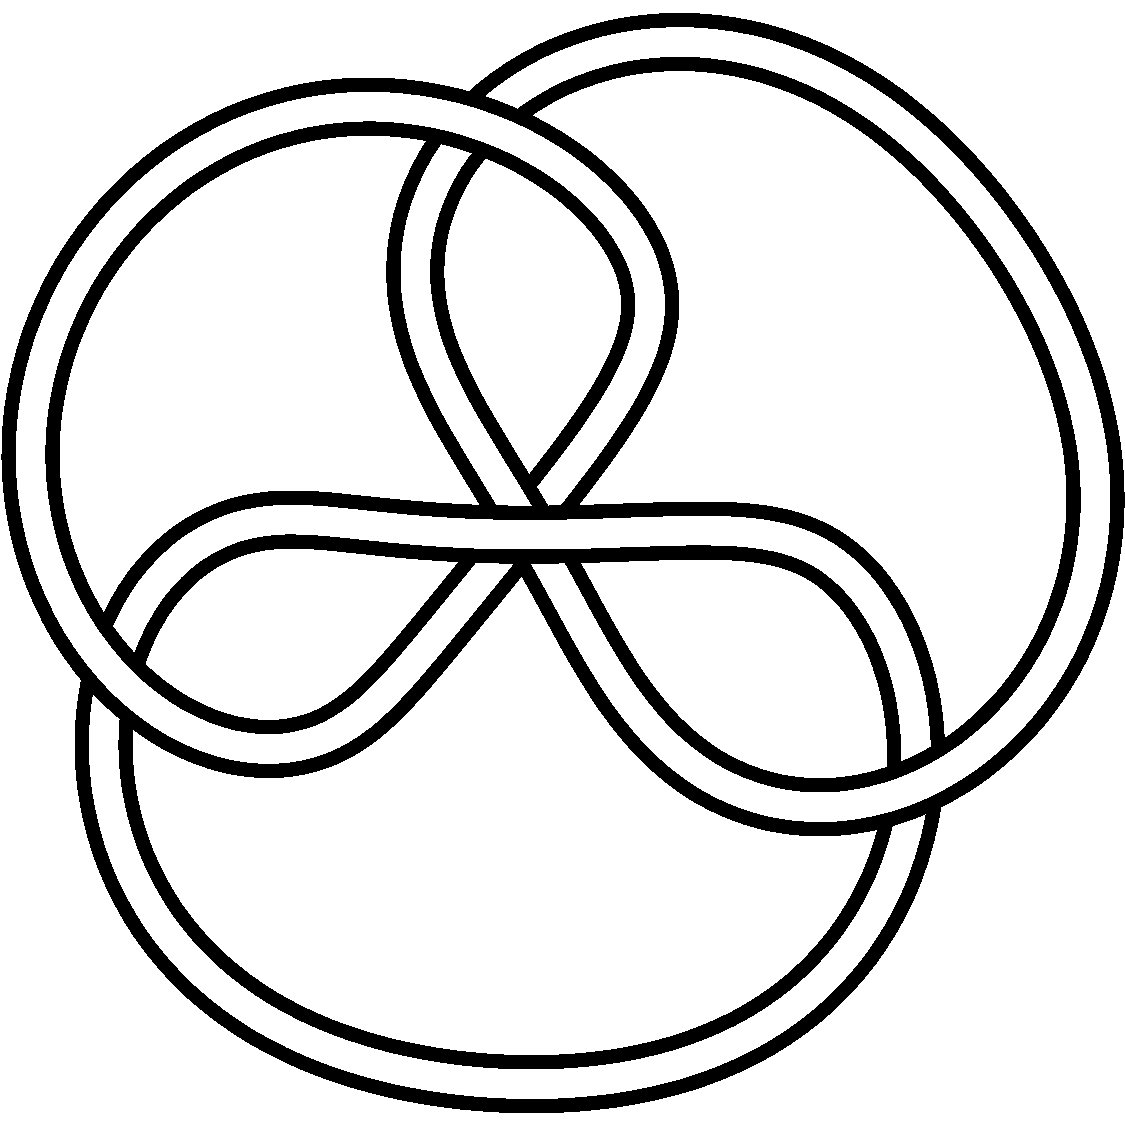
\includegraphics[scale=0.07,angle=0]{link6_3_3.pdf} 
& 
$
\displaystyle{%
\KR_{2} = \frac{1}{q^5}+\frac{1}{q^3}+\frac{t^2}{q^7}+\frac{t^3}{q^{11}}+\frac{2 t^4}{q^{13}}+\frac{3 t^4}{q^{11}}+\frac{t^4}{q^9}
}
$
\newline 
$
\displaystyle{%
\KR_{3} = \frac{1}{q^{10}}+\frac{1}{q^8}+\frac{1}{q^6}+\frac{t^2}{q^{12}}+\frac{t^2}{q^{10}}+\frac{t^3}{q^{18}}+\frac{t^3}{q^{16}}+\frac{2 t^4}{q^{20}}+\frac{5 t^4}{q^{18}}+\frac{6 t^4}{q^{16}}+\frac{4 t^4}{q^{14}}+\frac{t^4}{q^{12}}+\frac{t^6}{q^{24}}+\frac{2 t^6}{q^{22}}+\frac{2 t^6}{q^{20}}
}
$
\newline
$
\displaystyle{%
\qquad\qquad +\frac{t^6}{q^{18}}
}
$
\\
\hline
%%%%%%%%%%%%%%%%%%%%%%%%%%%%%%%%%%%%%%%%%%%%%%%%%%%%
$6_{3}^3\,\text{{\tiny (v2)}}$
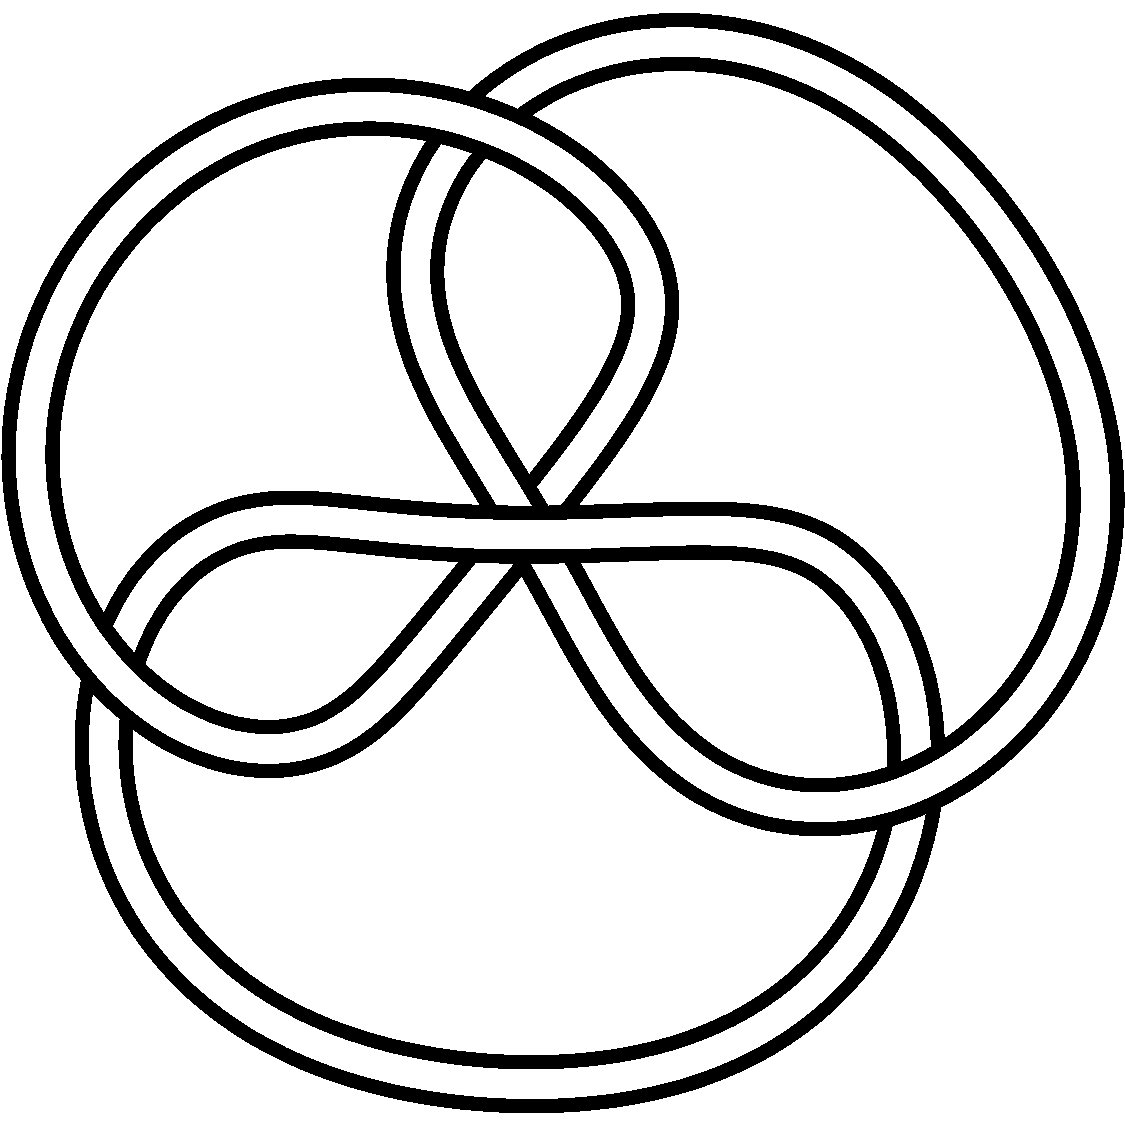
\includegraphics[scale=0.07,angle=0]{link6_3_3.pdf} 
& 
$
\displaystyle{%
\KR_{2} = \frac{2}{q}+3 q+q^3+\frac{q^7}{t^4}+\frac{q^9}{t^4}+\frac{q^5}{t^2}+\frac{q}{t}
}
$
\newline 
$
\displaystyle{%
\KR_{3} = 4+\frac{2}{q^2}+5 q^2+3 q^4+q^6+\frac{q^8}{t^4}+\frac{2 q^{10}}{t^4}+\frac{2 q^{12}}{t^4}+\frac{q^{14}}{t^4}+\frac{q^4}{t^2}+\frac{3 q^6}{t^2}+\frac{3 q^8}{t^2}+\frac{q^{10}}{t^2}+\frac{1}{t}+\frac{q^2}{t}
}
$
\\
\hline
%%%%%%%%%%%%%%%%%%%%%%%%%%%%%%%%%%%%%%%%%%%%%%%%%%%%
\end{longtable}
}




{\footnotesize 
\begin{longtable}{p{0.07\textwidth}|p{0.87\textwidth}} 
\caption{Reduced Khovanov-Rozansky $\sln$ invariants for prime links up to 6 crossings} \\
\label{reducedKR}
link $L$ & $\overline{\KR}_{N}(L)$ \\
\hline\hline
\endfirsthead
link $L$ & $\overline{\KR}_{N}(L)$ \\
\hline\hline
\endhead
\hline\hline
\endfoot
%%%%%%%%%%%%%%%%%%%%%%%%%%%%%%%%%%%%%%%%%%%%%%%%%%%%
$2_{1}^2\,\text{{\tiny (v1\&v2)}}$ 
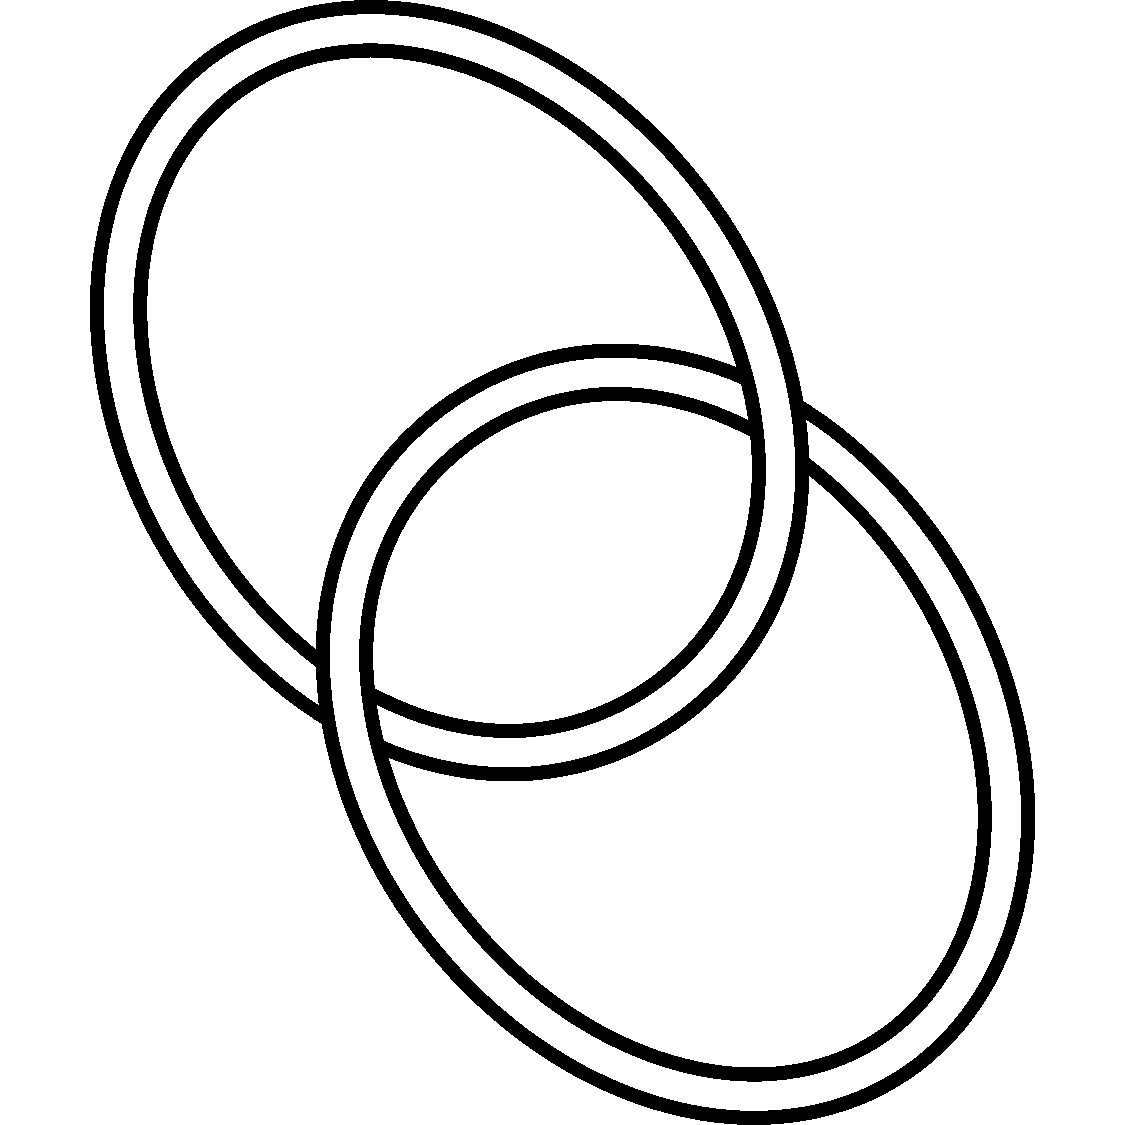
\includegraphics[scale=0.07,angle=0]{link2_1_2.pdf} 
& 
$
\displaystyle{%
q^{1-N} + \frac{q^{-N-1}-q^{1-3 N}}{q^2-1} t^2
}
$
\newline\newline\newline\newline
Checked up to $N=18$. Extends result of~\cite{r0508510} to $N=3$ and $N=4$. 
\\
\hline
%%%%%%%%%%%%%%%%%%%%%%%%%%%%%%%%%%%%%%%%%%%%%%%%%%%%
$3_{1}$ 
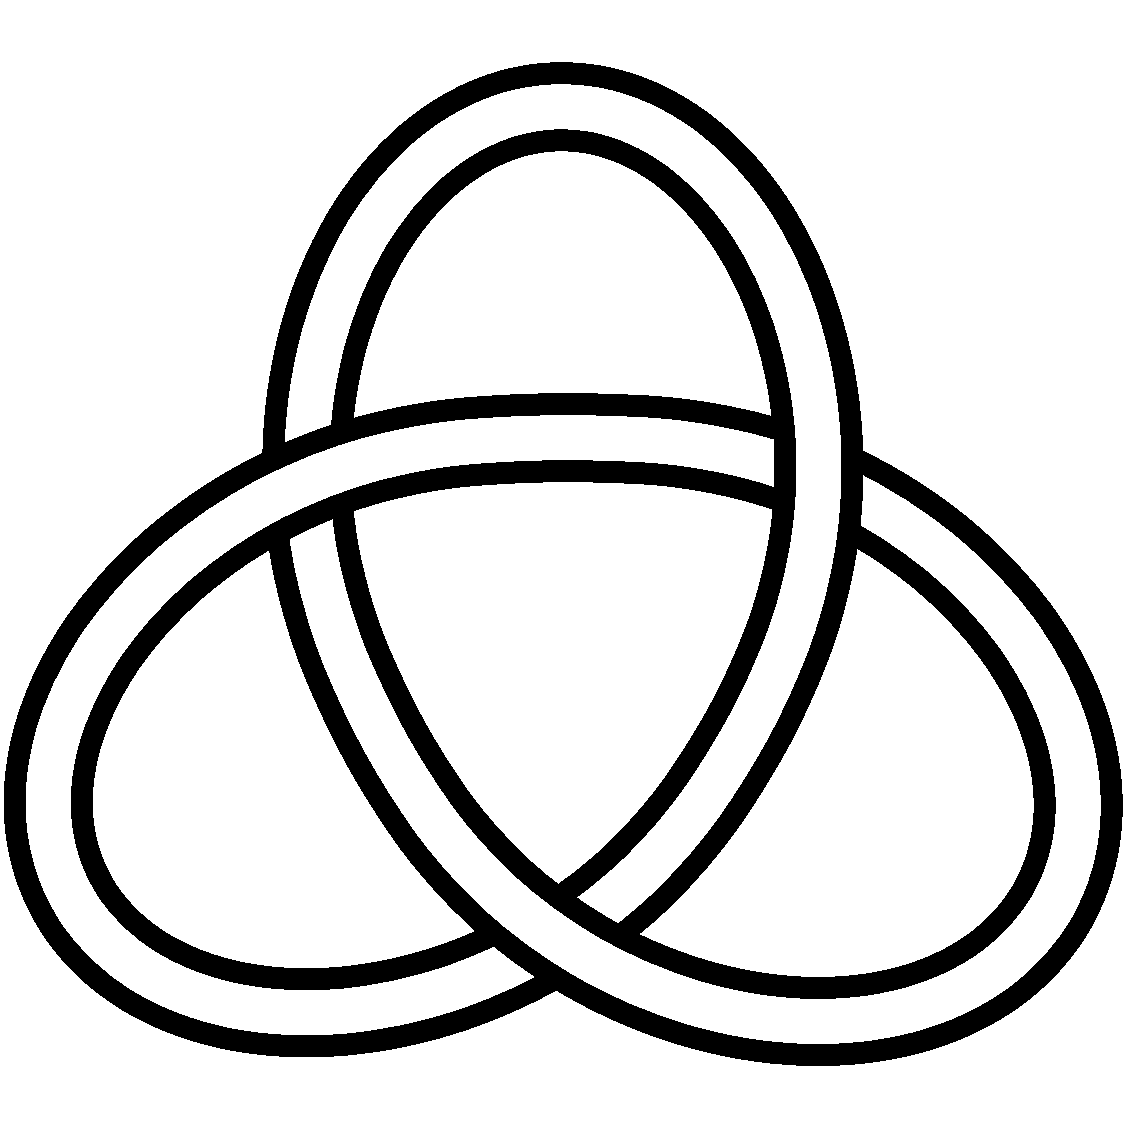
\includegraphics[scale=0.07,angle=0]{knot3_1.pdf} 
& 
$
\displaystyle{%
q^{4N} t^{-3} + q^{2 + 2N} t^{-2} + q^{-2 + 2N}
}
$
\newline\newline\newline\newline
Checked up to $N=16$. Agrees with results of~\cite{r0508510, r0607544}. 
\\
\hline
%%%%%%%%%%%%%%%%%%%%%%%%%%%%%%%%%%%%%%%%%%%%%%%%%%%%
$4_{1}$ 
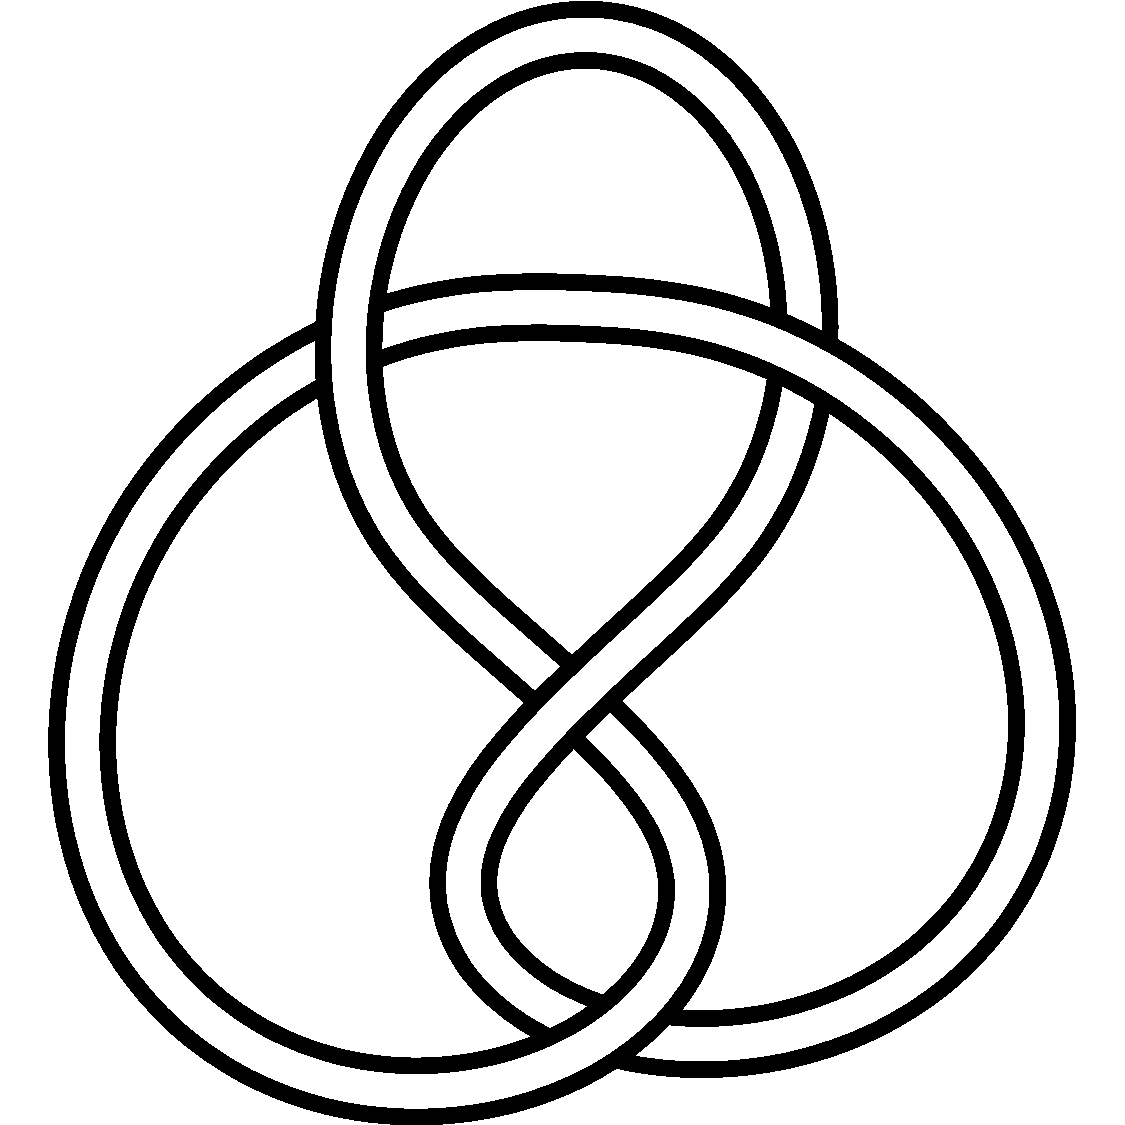
\includegraphics[scale=0.07,angle=0]{knot4_1.pdf} 
& 
$
\displaystyle{%
1 + q^{2 N} t^{-2} + q^2 t^{-1} + t q^{-2} + q^{-2 N} t^2
}
$
\newline\newline\newline\newline
Checked up to TODO. Agrees with results of~\cite{r0508510, r0607544}. 
\\
\hline
%%%%%%%%%%%%%%%%%%%%%%%%%%%%%%%%%%%%%%%%%%%%%%%%%%%%
$4_{1}^2\,\text{{\tiny (v1)}}$ 
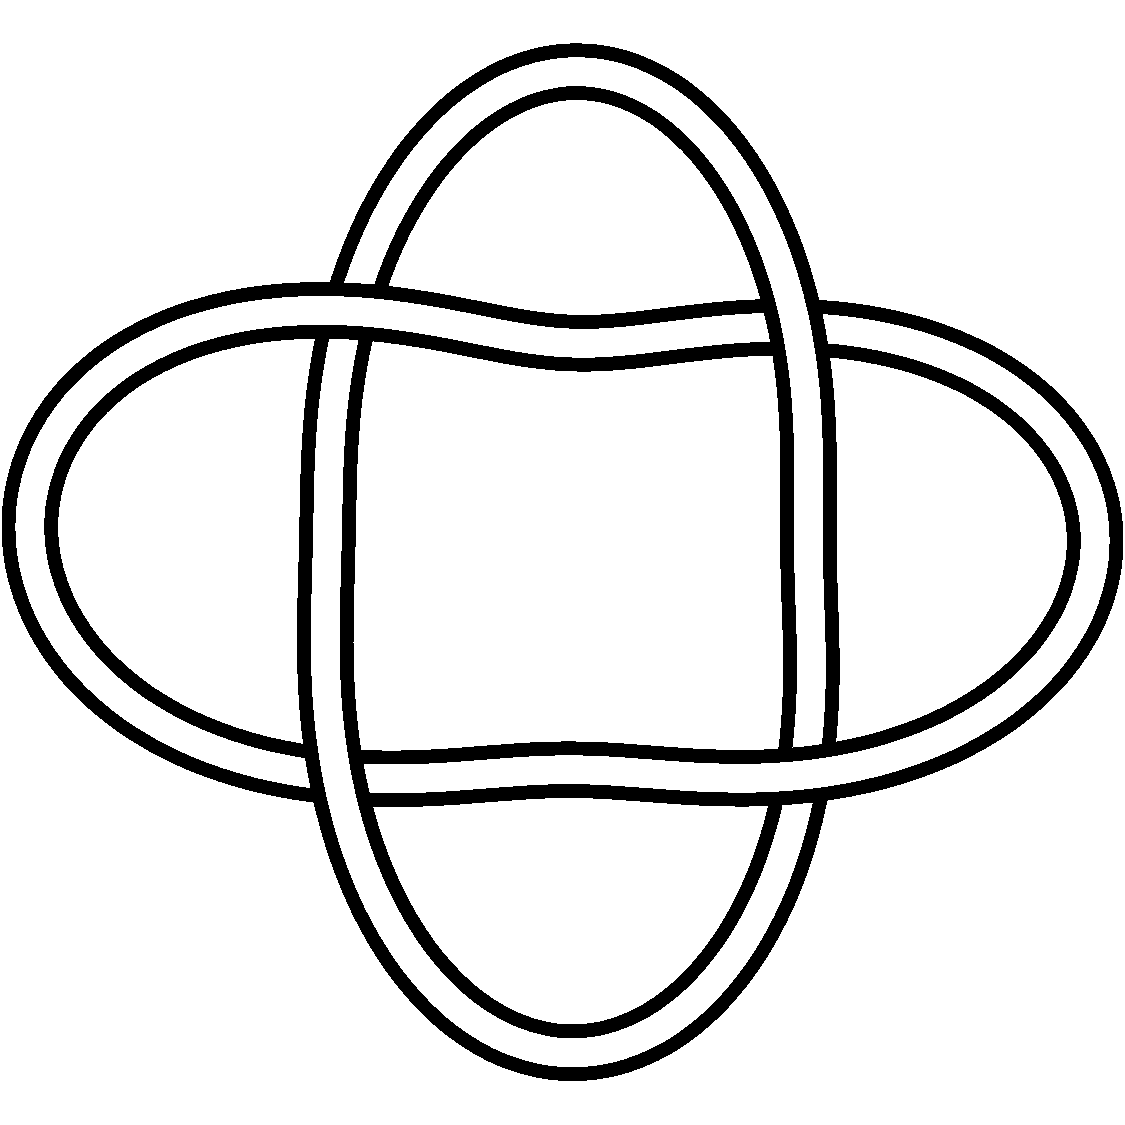
\includegraphics[scale=0.07,angle=0]{link4_1_2.pdf} 
& 
$
\displaystyle{%
% OLD OLD: \sum_{j=0}^{N-2} t^4 q^{2j + 2 - 6N}  + t^2 q^{2 - 4N} + t q^{4-4N} + q^{2-2N} 
q^{1-N}+q^{-N-1} t+q^{1-3 N} t^2-\frac{q^{1-5N} t^4}{q^2-1}+\frac{q^{-3 N-1} t^4}{q^2-1}
}
$
\newline\newline\newline\newline
Checked up to $N=6$. Extends result of~\cite{r0508510} to $N=3$ and $N=4$. 
\\
\hline
%%%%%%%%%%%%%%%%%%%%%%%%%%%%%%%%%%%%%%%%%%%%%%%%%%%%
$4_{1}^2\,\text{{\tiny (v2)}}$ 
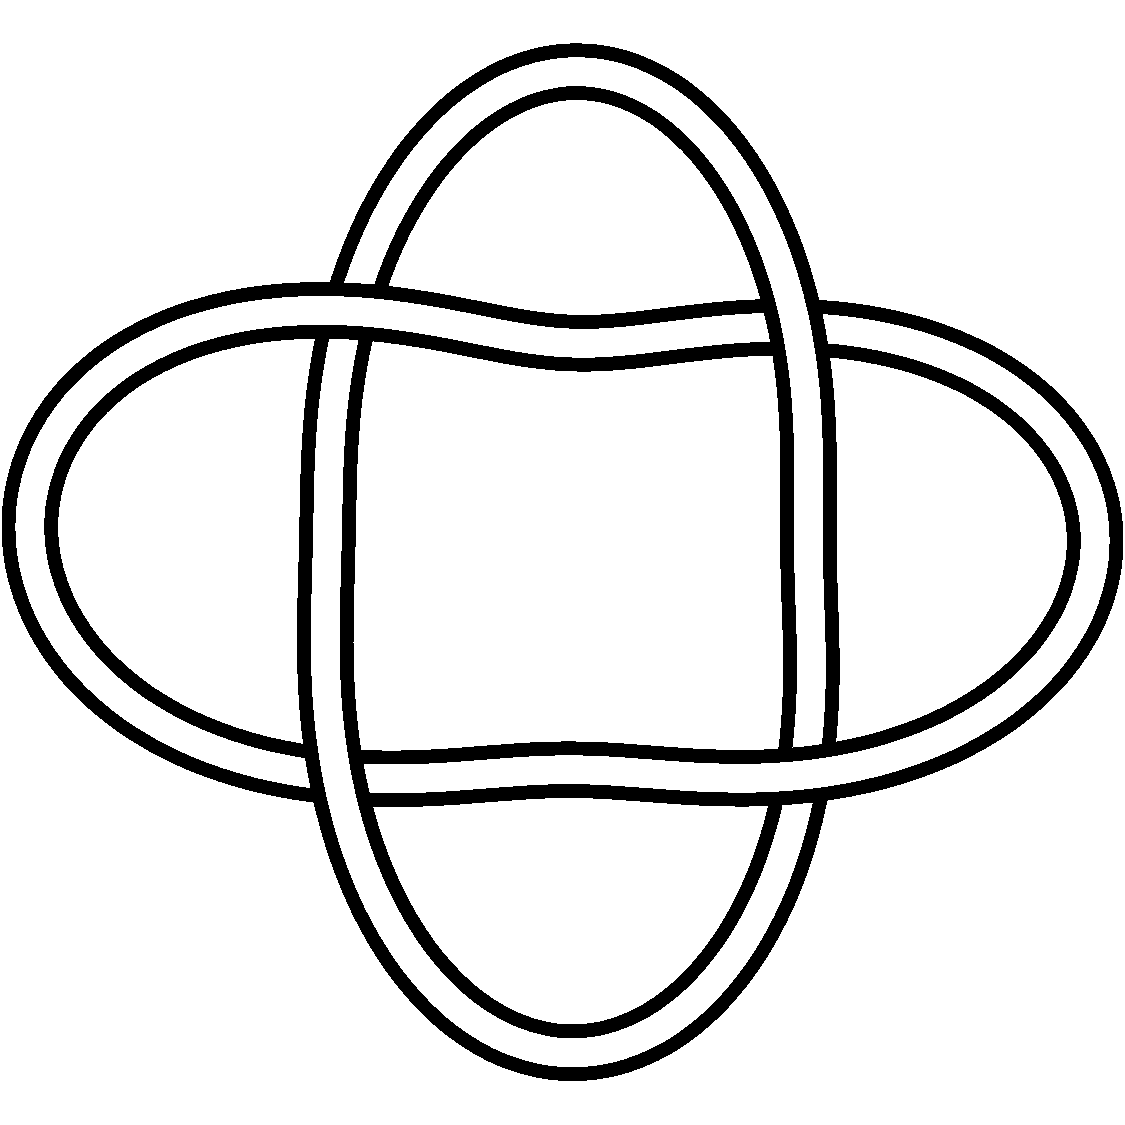
\includegraphics[scale=0.07,angle=0]{link4_1_2.pdf} 
& 
$
\displaystyle{%
%OLD OLD: \sum_{j=0}^{N-2} t^4 q^{2j-6N} + t^3 q^{2-6N} + t^2 q^{-4N} + t q^{4-4N} + q^{8-2N} 
q^{3 N-3}-\frac{q^{3N+5}}{\left(q^2-1\right) t^4}+\frac{q^{5 N+3}}{\left(q^2-1\right) t^4}+\frac{q^{5 N-1}}{t^3}+\frac{q^{3 N+1}}{t^2}
}
$
\newline\newline\newline\newline
Checked up to $N=8$. Extends result of~\cite{r0508510} to $N=3$ and $N=4$. 
\\
\hline
%%%%%%%%%%%%%%%%%%%%%%%%%%%%%%%%%%%%%%%%%%%%%%%%%%%%
$5_{1}$ 
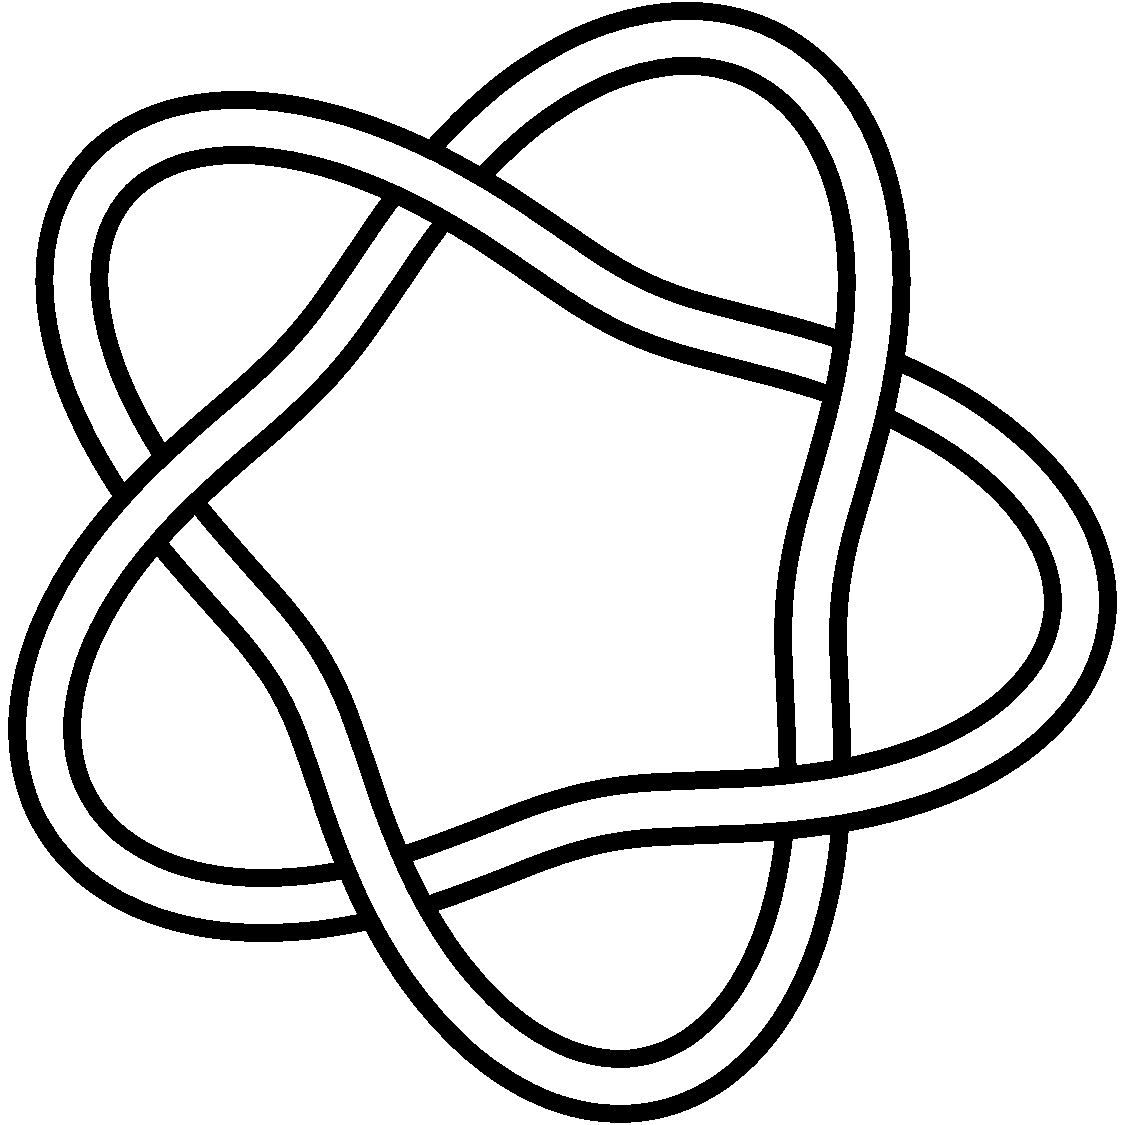
\includegraphics[scale=0.07,angle=0]{knot5_1.pdf} 
& 
$
\displaystyle{%
q^{4 - 4 N} + q^{-4 N} t^2 + q^{2 - 6 N} t^3 + q^{-4 - 4 N} t^4 +  q^{-2 - 6 N} t^5
}
$
\newline\newline\newline\newline
Checked up to $N=7$. Agrees with results of~\cite{r0508510, r0607544}. 
\\
\hline
%%%%%%%%%%%%%%%%%%%%%%%%%%%%%%%%%%%%%%%%%%%%%%%%%%%%
$5_{2}$ 

\includegraphics[scale=0.07,angle=0]{knot5_2.pdf} 
& 
$
\displaystyle{%
q^{2 - 2 N} + q^{-2 N} t + q^{2 - 4 N} t^2 + q^{-2 - 2 N} t^2 + q^{-4 N} t^3 + q^{-2 - 4 N} t^4 + q^{-6 N} t^5
}
$
\newline\newline\newline\newline
Checked up to $N=4$. Agrees with results of~\cite{r0508510, r0607544}. 
\\
\hline
%%%%%%%%%%%%%%%%%%%%%%%%%%%%%%%%%%%%%%%%%%%%%%%%%%%%
$5_{1}^2\,\text{{\tiny (v1\&v2)}}$ 
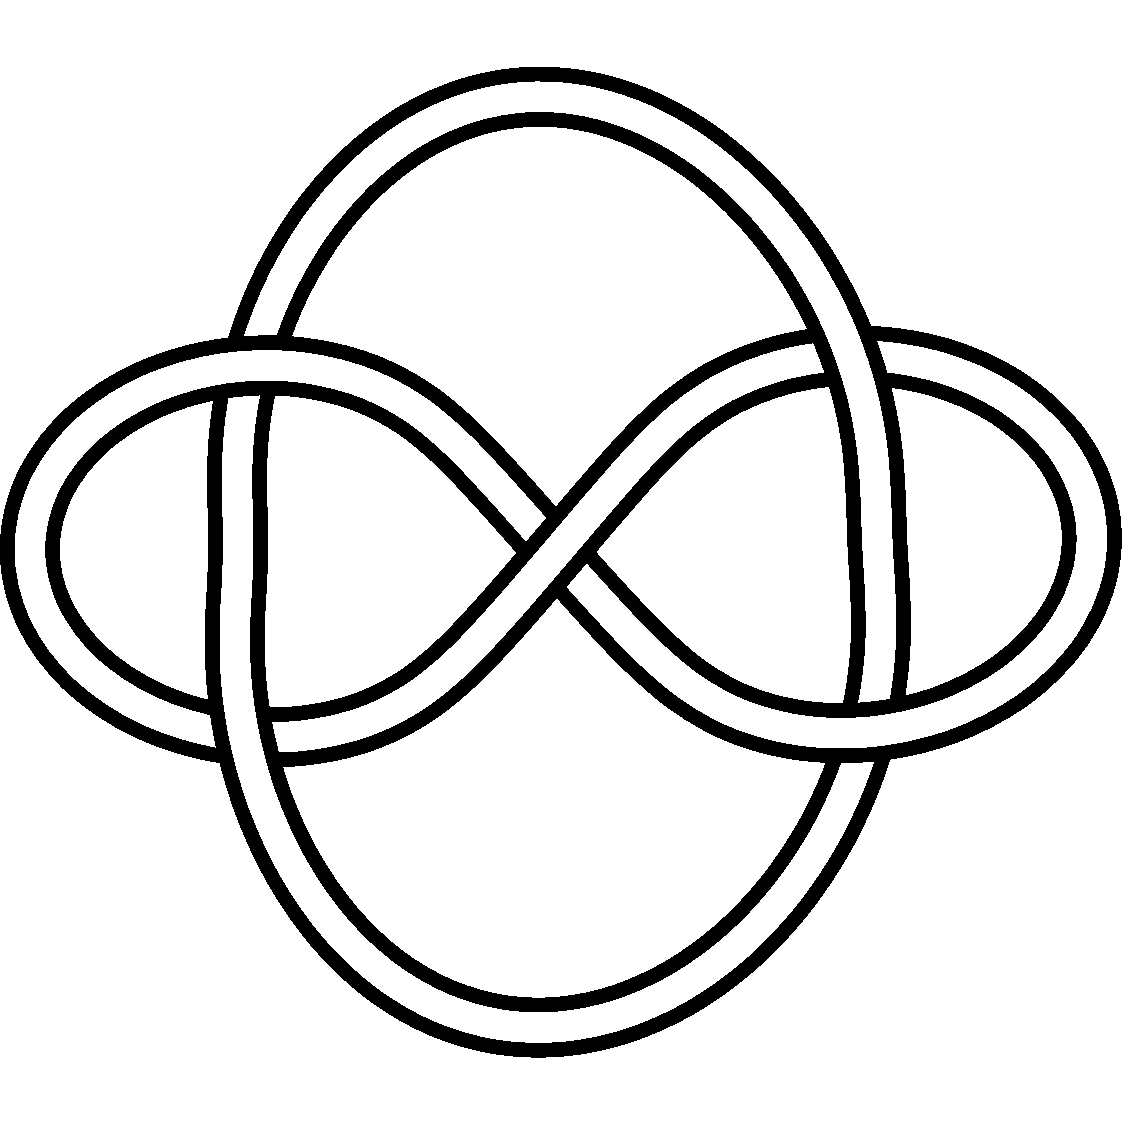
\includegraphics[scale=0.07,angle=0]{link5_1_2.pdf} 
& 
$
\displaystyle{%
q^{1-N}+\frac{q^{N-1} - q^{1-N}}{q^2-1}+\frac{q^{N+1}}{t^2}+\frac{q^{3-N}}{t}+q^{-N-1} t+q^{1-3N} t^2+q^{-N-3} t^2+q^{-3 N-1} t^3
}
$
\newline\newline\newline\newline
Checked up to $N=4$. Extends result of~\cite{r0508510} to $N=3$ and $N=4$. 
\\
\hline
%%%%%%%%%%%%%%%%%%%%%%%%%%%%%%%%%%%%%%%%%%%%%%%%%%%%
$6_{1}$ 
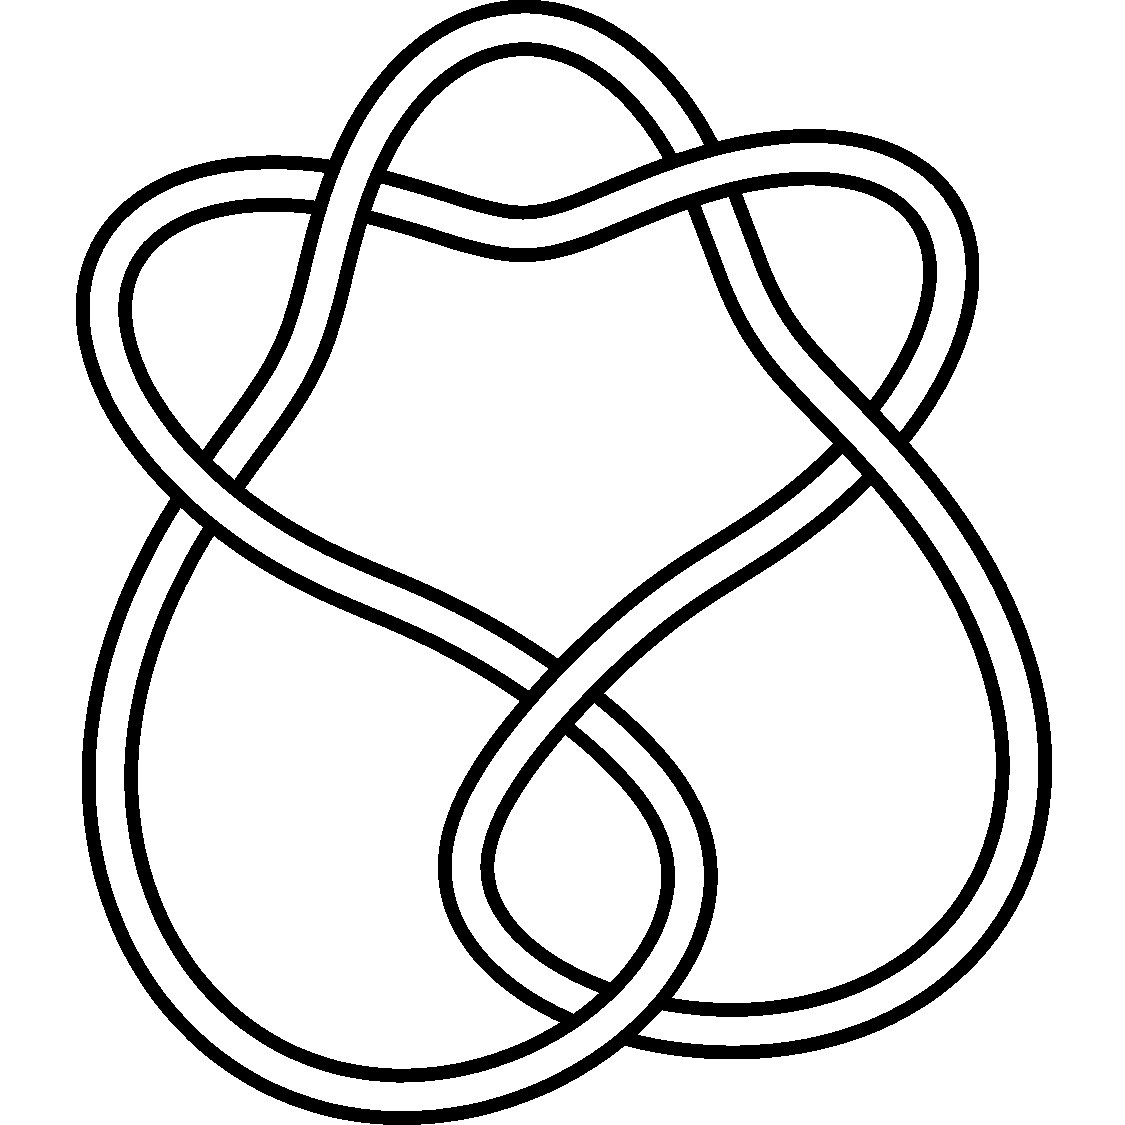
\includegraphics[scale=0.07,angle=0]{knot6_1.pdf} 
& 
$
\displaystyle{%
2+q^{2 N}t^{-2}+q^2 t^{-1}+ t q^{-2} + q^{2-2N} t+q^{-2 N} t^2+q^{-2N-2} t^3+q^{-4 N} t^4
}
$
\newline\newline\newline\newline
Checked up to TODO (so far only $N=2$). Agrees with results of~\cite{r0508510, r0607544}. 
\\
\hline
%%%%%%%%%%%%%%%%%%%%%%%%%%%%%%%%%%%%%%%%%%%%%%%%%%%%
$6_{2}$ 
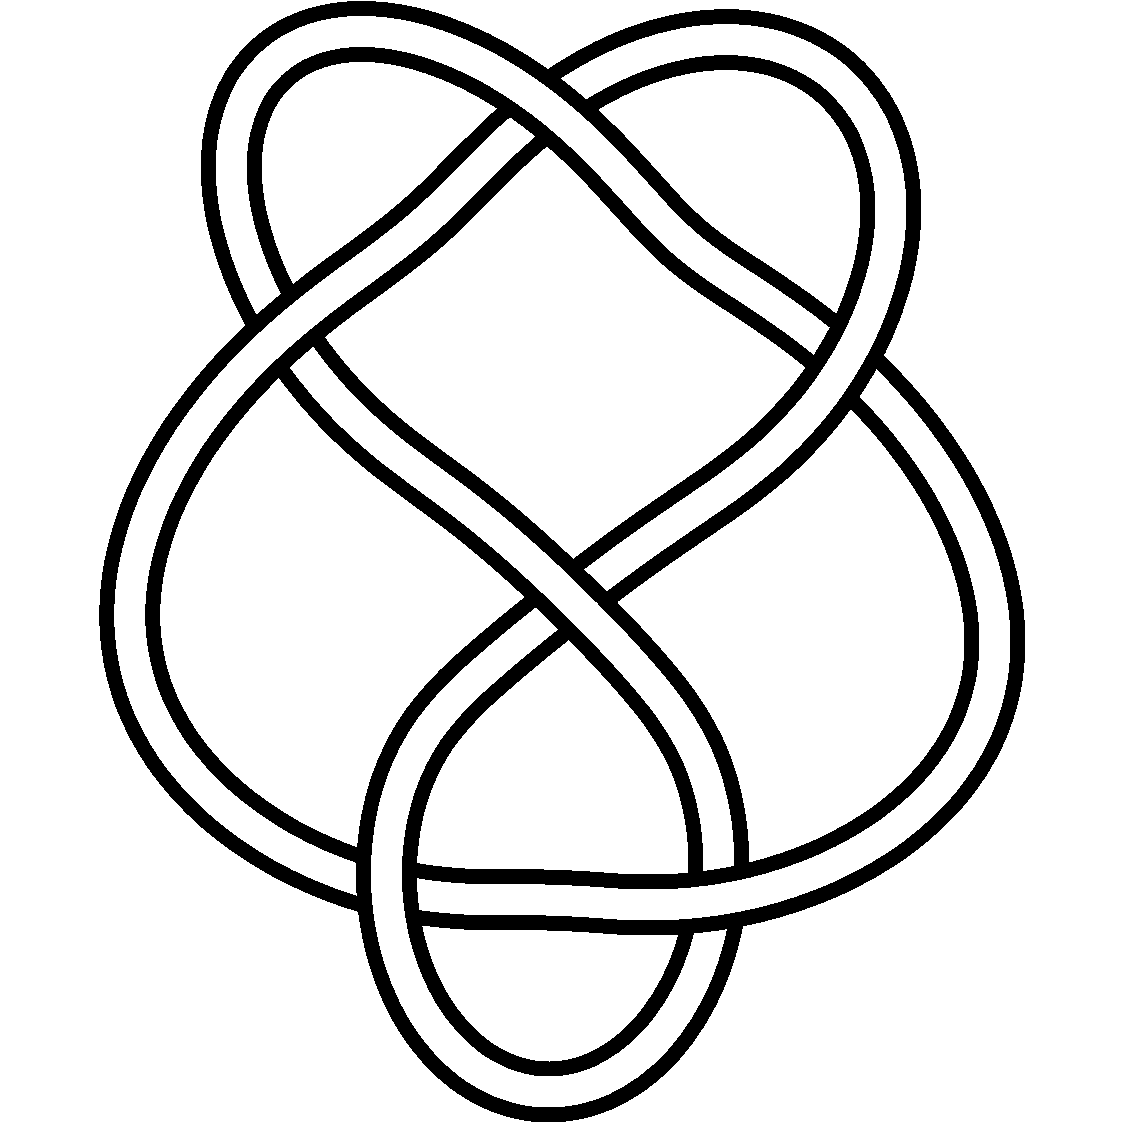
\includegraphics[scale=0.07,angle=0]{knot6_2.pdf} 
& 
$
\displaystyle{%
q^{-2} + q^{2-2 N} + q^2t^{-2} + q^{4-2 N} t^{-1} + 2 q^{-2 N} t+q^{2-4 N} t^2+q^{-N-2} t^2+q^{-4 N} t^3+q^{-2N-4} t^3+q^{-4N-2} t^4
}
$
\newline\newline\newline\newline
Checked up to $N=4$. Agrees with results of~\cite{r0508510, r0607544}. 
\\
\hline
%%%%%%%%%%%%%%%%%%%%%%%%%%%%%%%%%%%%%%%%%%%%%%%%%%%%
$6_{3}$ 

\includegraphics[scale=0.07,angle=0]{knot6_3.pdf} 
& 
$
\displaystyle{%
3+q^{2N+2} t^{-3} + q^4t^{-2}+ q^{2 N}t^{-2}+ q^2 t^{-1}+ q^{2 N-2}t^{-1}+ t q^{-2}+q^{2-2 N} t+ t^2q^{-4}+q^{-2 N} t^2+q^{-2N-2} t^3
}
$
\newline\newline\newline\newline
Checked up to TODO (so far only up to $N=3$). Agrees with results of~\cite{r0508510, r0607544}. 
\\
\hline
%%%%%%%%%%%%%%%%%%%%%%%%%%%%%%%%%%%%%%%%%%%%%%%%%%%%
$6_{1}^2\,\text{{\tiny (v1)}}$ 
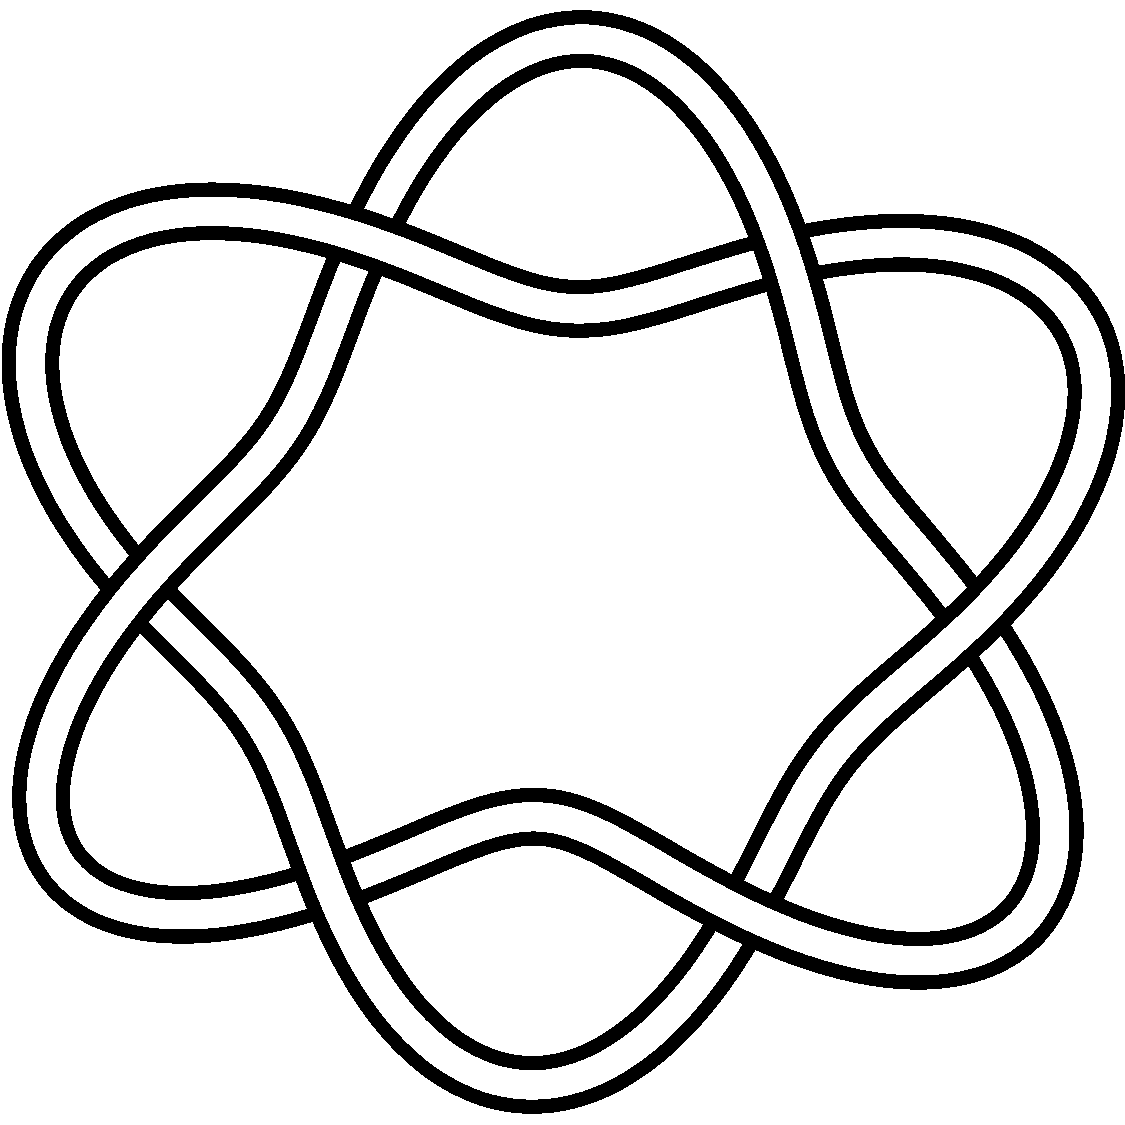
\includegraphics[scale=0.07,angle=0]{link6_1_2.pdf} 
& 
$
\displaystyle{%
q^{5 N-5} \left(1+\frac{q^{2N+10}-q^{12}}{\left(q^2-1\right) t^6}+\frac{q^{2 N+6}}{t^5}+\frac{q^8}{t^4}+\frac{q^{2 N+2}}{t^3}+\frac{q^4}{t^2}\right)
}
$
\newline\newline\newline\newline
Checked up to $N=5$. Extends result of~\cite{r0508510} to $N=3$ and $N=4$. 
\\
\hline
%%%%%%%%%%%%%%%%%%%%%%%%%%%%%%%%%%%%%%%%%%%%%%%%%%%%
$6_{1}^2\,\text{{\tiny (v2)}}$ 
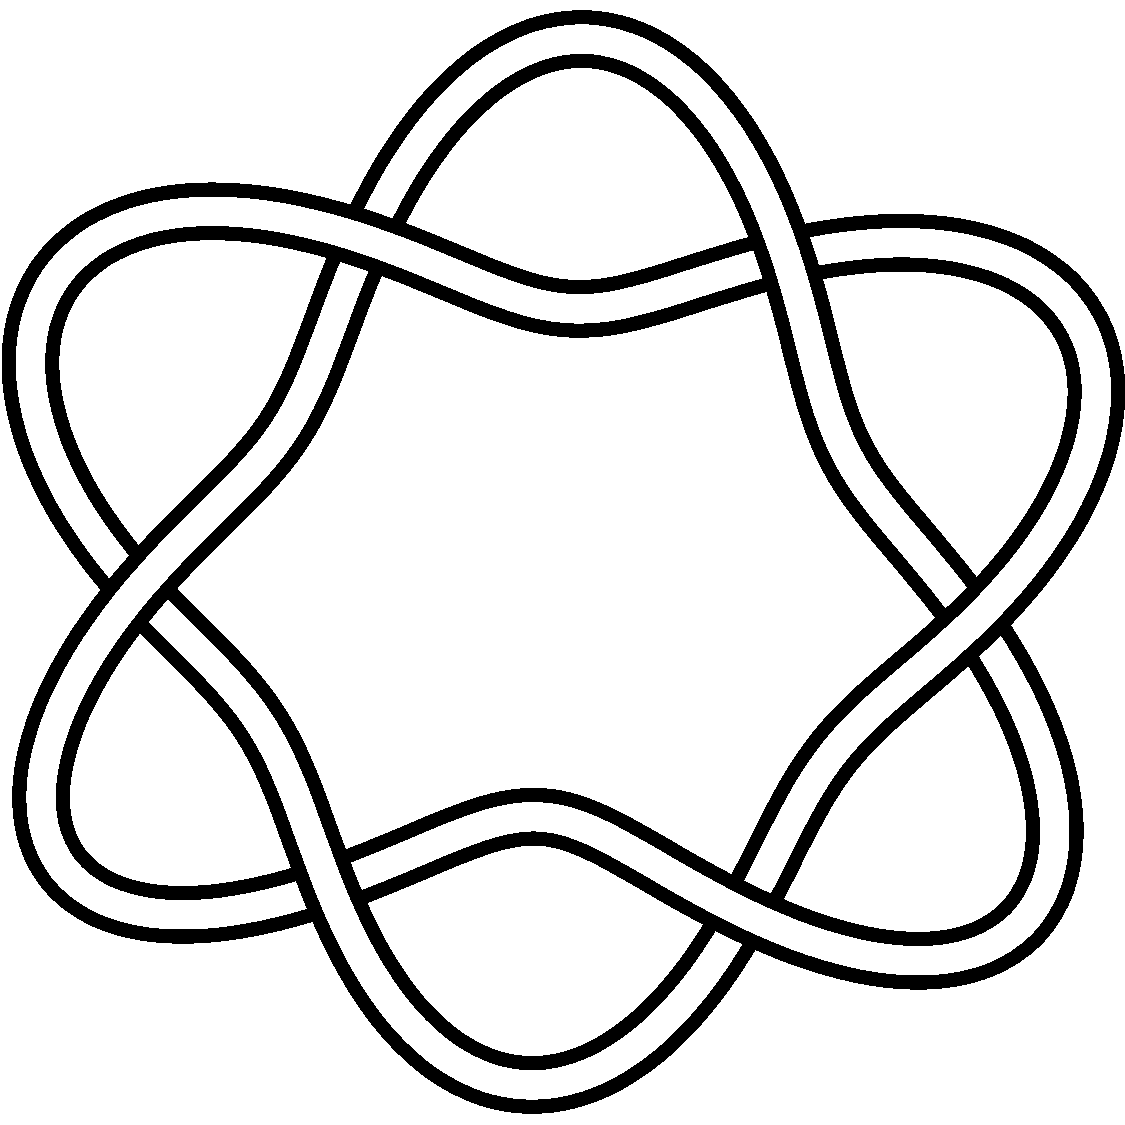
\includegraphics[scale=0.07,angle=0]{link6_1_2.pdf} 
& 
$
\displaystyle{%
q^{-7 N-1} \left(q^{6 N+2}+q^{6 N} t+q^{4 N+2} t^2+q^{4 N} t^3+q^{2 N+2} t^4+\frac{q^{2 N} -q^2 }{q^2-1} t^6\right)
}
$
\newline\newline\newline\newline
Checked up to $N=3$. Extends result of~\cite{r0508510} to $N=3$.
\\
\hline
%%%%%%%%%%%%%%%%%%%%%%%%%%%%%%%%%%%%%%%%%%%%%%%%%%%%
$6_{1}^3\,\text{{\tiny (v1)}}$ 
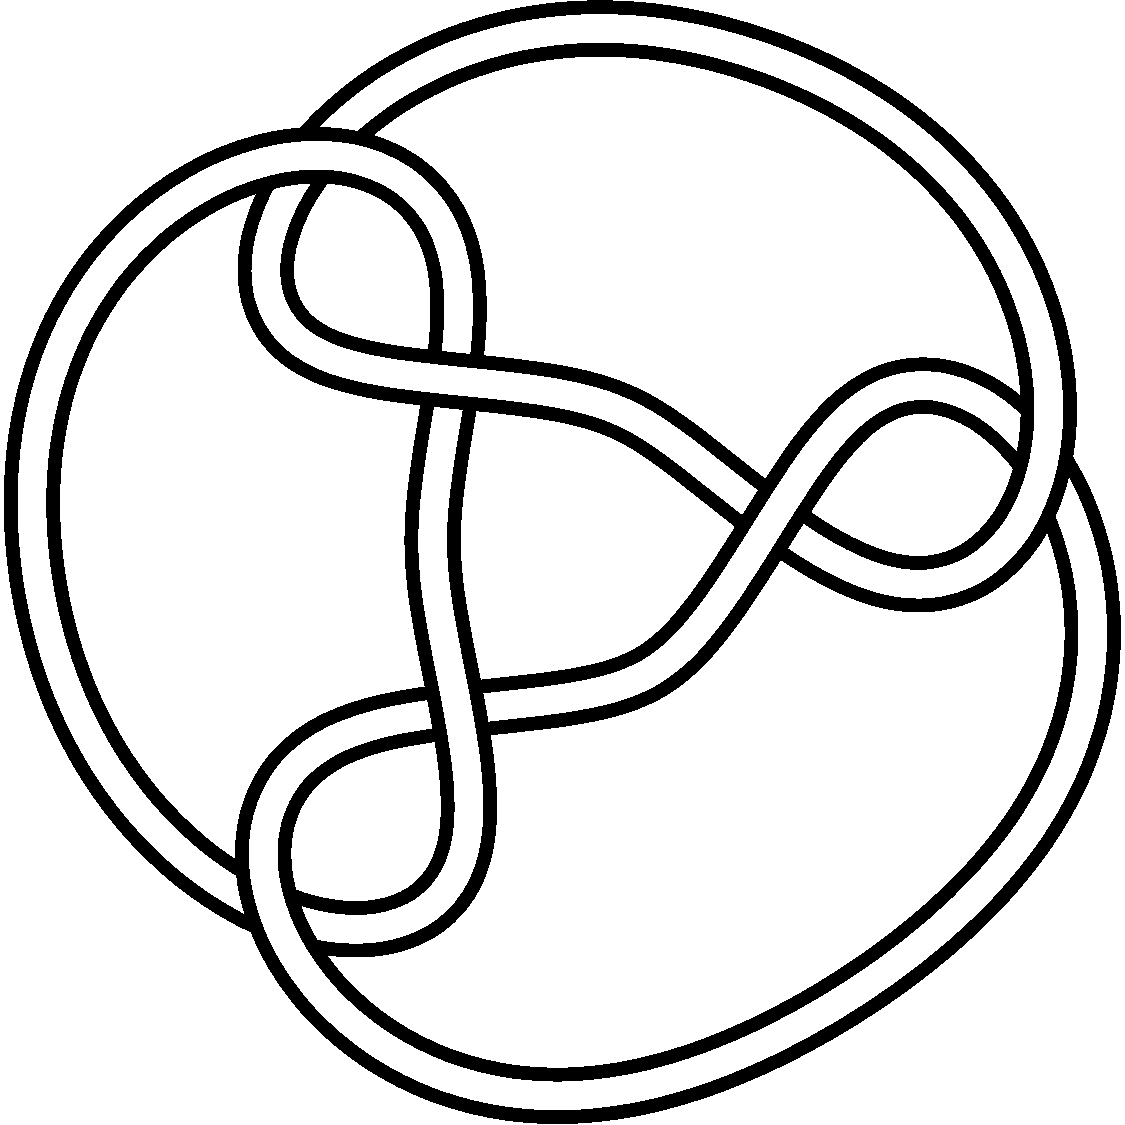
\includegraphics[scale=0.07,angle=0]{link6_1_3.pdf} 
& 
$
\displaystyle{%
\overline{\KR}_{2} = \frac{1}{q^2}+\frac{2 t}{q^4}+\frac{3 t^2}{q^6}+\frac{t^3}{q^8}+\frac{3 t^4}{q^{10}}+\frac{t^5}{q^{12}}+\frac{t^6}{q^{14}}
}
$
\newline 
$
\displaystyle{%
\overline{\KR}_{3} = \frac{1}{q^4}+\frac{2 t}{q^6}+\frac{2 t^2}{q^{10}}+\frac{t^2}{q^8}+\frac{t^3}{q^{12}}+\frac{3 t^4}{q^{16}}+\frac{3 t^4}{q^{14}}+\frac{t^5}{q^{16}}+\frac{t^6}{q^{22}}+\frac{2 t^6}{q^{20}}
}
$
\\
\hline
%%%%%%%%%%%%%%%%%%%%%%%%%%%%%%%%%%%%%%%%%%%%%%%%%%%%
$6_{1}^3\,\text{{\tiny (v2)}}$ 
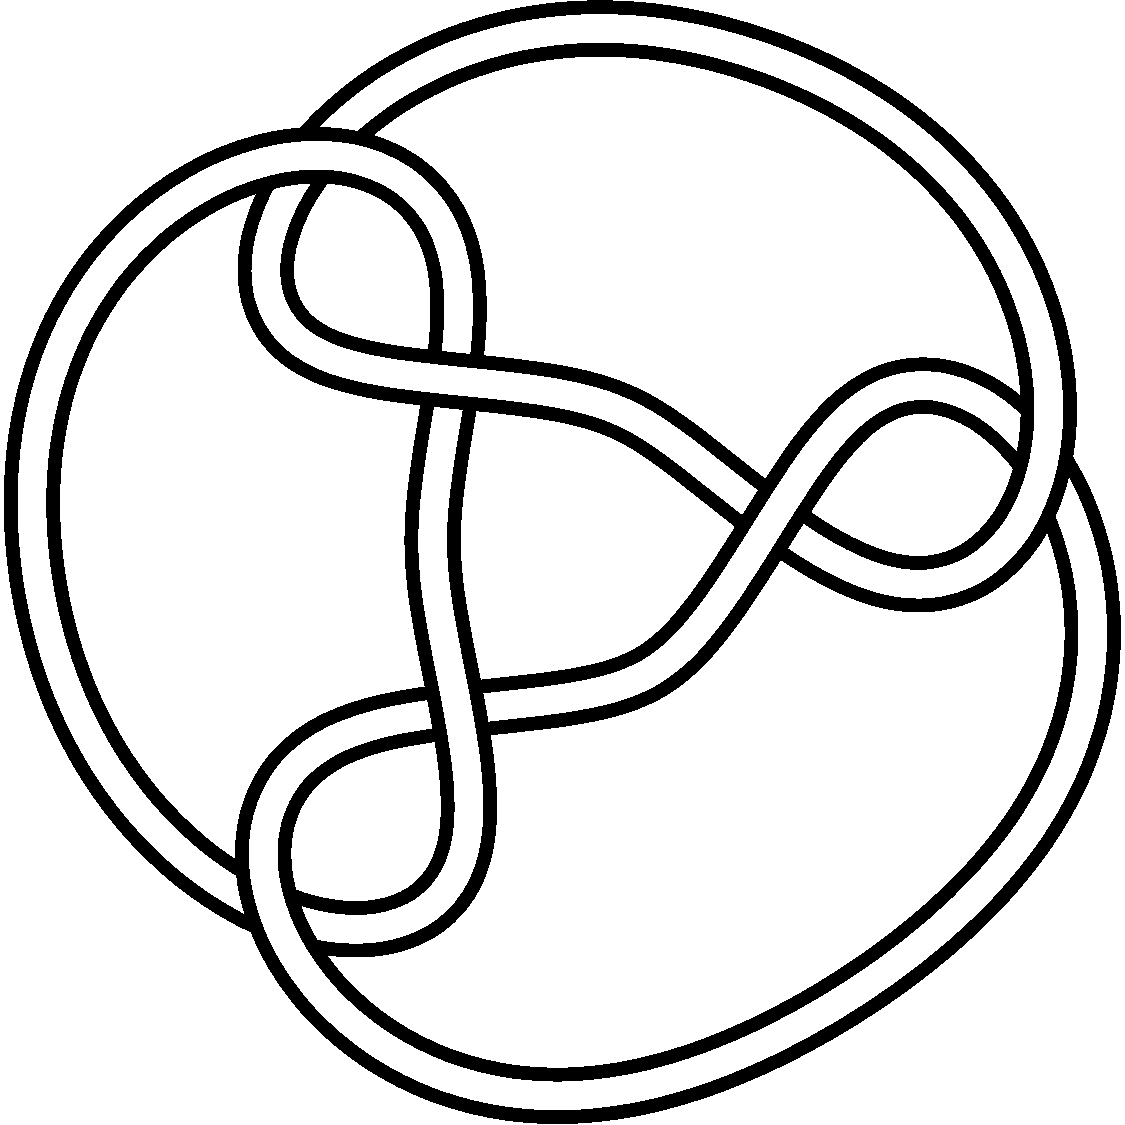
\includegraphics[scale=0.07,angle=0]{link6_1_3.pdf} 
& 
$
\displaystyle{%
\overline{\KR}_{2} = 3 q^2+\frac{q^{10}}{t^4}+\frac{2 q^8}{t^3}+\frac{3 q^6}{t^2}+\frac{q^4}{t}+t+\frac{t^2}{q^2}
}
$
\newline 
$
\displaystyle{%
\overline{\KR}_{3} = 2 q^2+3 q^4+\frac{q^{12}}{t^4}+\frac{q^{14}}{t^4}+\frac{2 q^{12}}{t^3}+\frac{q^6}{t^2}+\frac{3 q^8}{t^2}+\frac{q^{10}}{t^2}+\frac{q^6}{t}+q^2 t+\frac{t^2}{q^2}
}
$
\\
\hline
%%%%%%%%%%%%%%%%%%%%%%%%%%%%%%%%%%%%%%%%%%%%%%%%%%%%
$6_{2}^2\,\text{{\tiny (v1)}}$ 
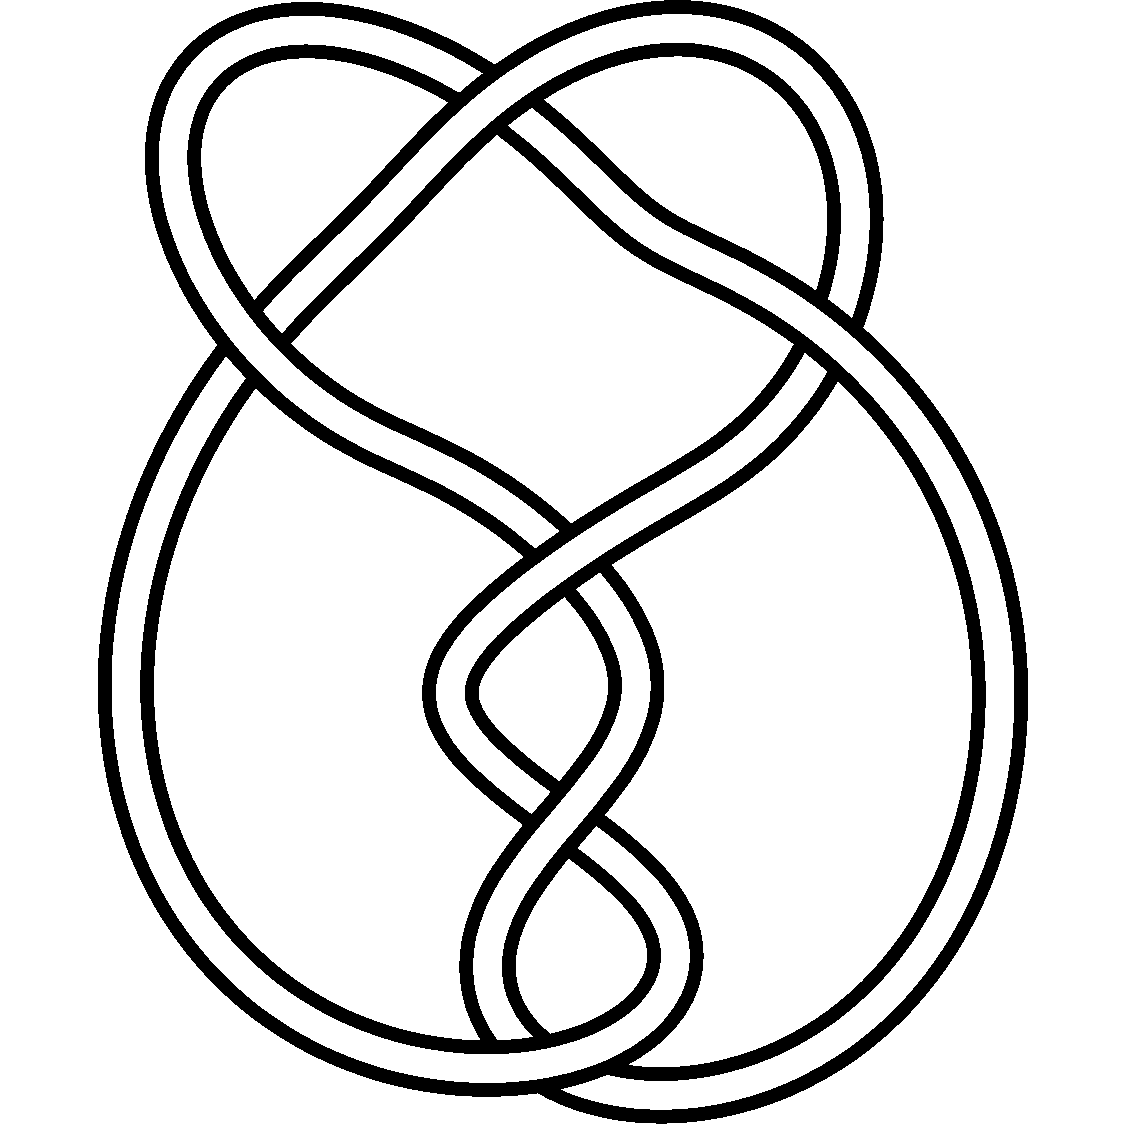
\includegraphics[scale=0.07,angle=0]{link6_2_2.pdf} 
& 
$
\displaystyle{%
q^{-7 N-3} \left(q^{4 N+6}+q^{4 N+4} t+q^{2 N+6} t^2+q^{4 N+2} t^2+q^{4 N} t^3+q^{2 N+4} t^3+2 q^{2 N+2} t^4+q^4 t^5+\frac{q^{2 N} -q^2}{q^2-1} t^6\right)
}
$
\newline\newline\newline\newline
Checked up to $N=4$. Extends result of~\cite{r0508510} to $N=3$ and $N=4$.
\\
\hline
%%%%%%%%%%%%%%%%%%%%%%%%%%%%%%%%%%%%%%%%%%%%%%%%%%%%
$6_{2}^2\,\text{{\tiny (v2)}}$ 
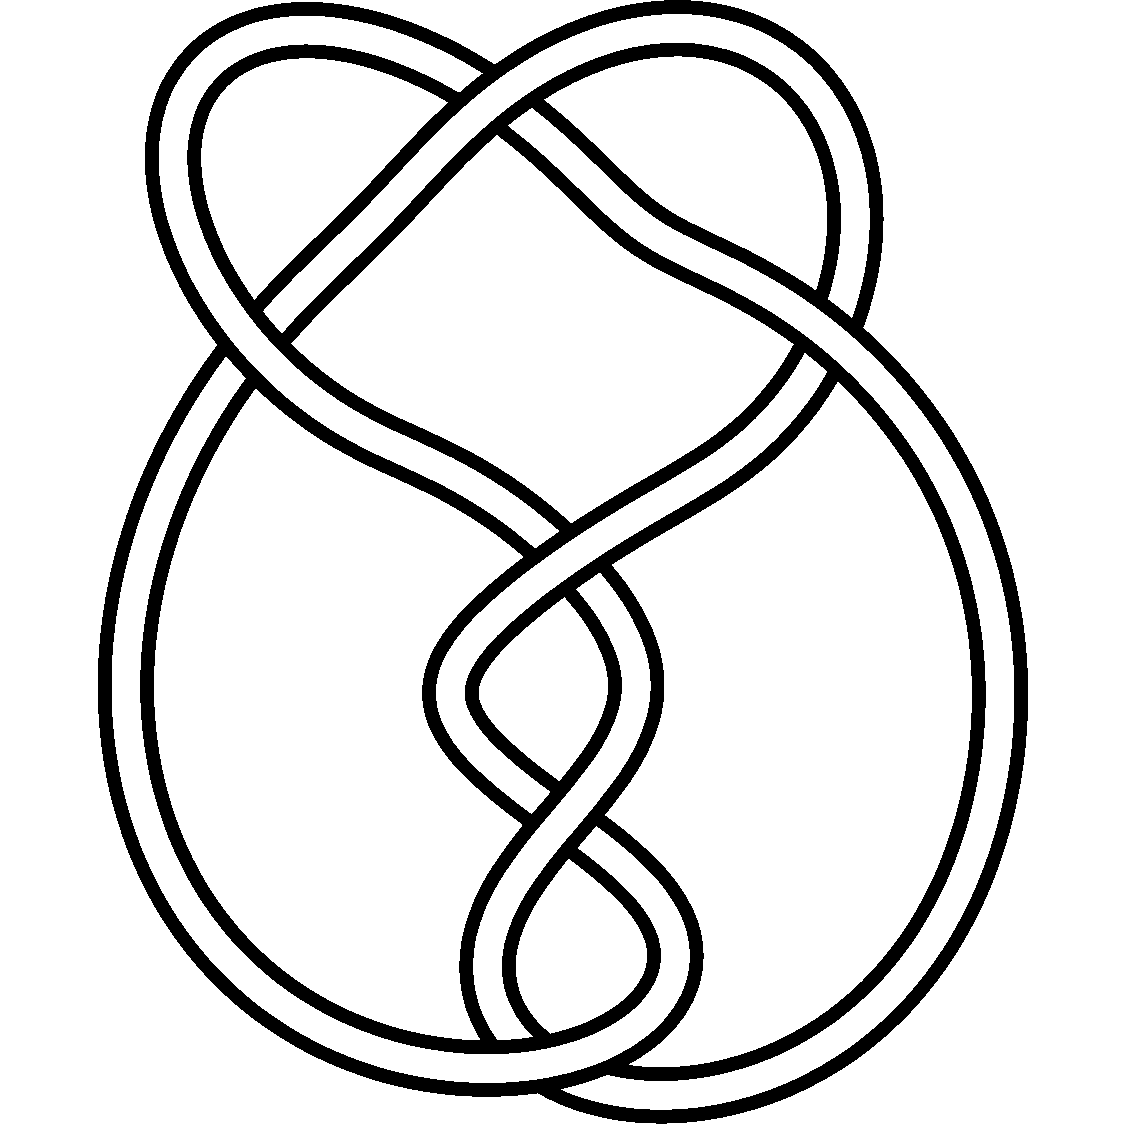
\includegraphics[scale=0.07,angle=0]{link6_2_2.pdf} 
& 
$
\displaystyle{%
q^{3 N-3}+\frac{q^{7 N+3}-q^{5 N+5}}{\left(q^2-1\right) t^6}+\frac{q^{7 N-1}}{t^5}+\frac{2 q^{5 N+1}}{t^4}+\frac{q^{3 N+3}}{t^3}+\frac{q^{5 N-1}}{t^3}+\frac{q^{3 N+1}}{t^2}+\frac{q^{5 N-3}}{t^2}+\frac{q^{3 N-1}}{t}
}
$
\newline\newline\newline\newline
Checked up to $N=4$. Extends result of~\cite{r0508510} to $N=3$ and $N=4$.
\\
\hline
%%%%%%%%%%%%%%%%%%%%%%%%%%%%%%%%%%%%%%%%%%%%%%%%%%%%
$6_{2}^3\,\text{{\tiny (v1)}}$ 
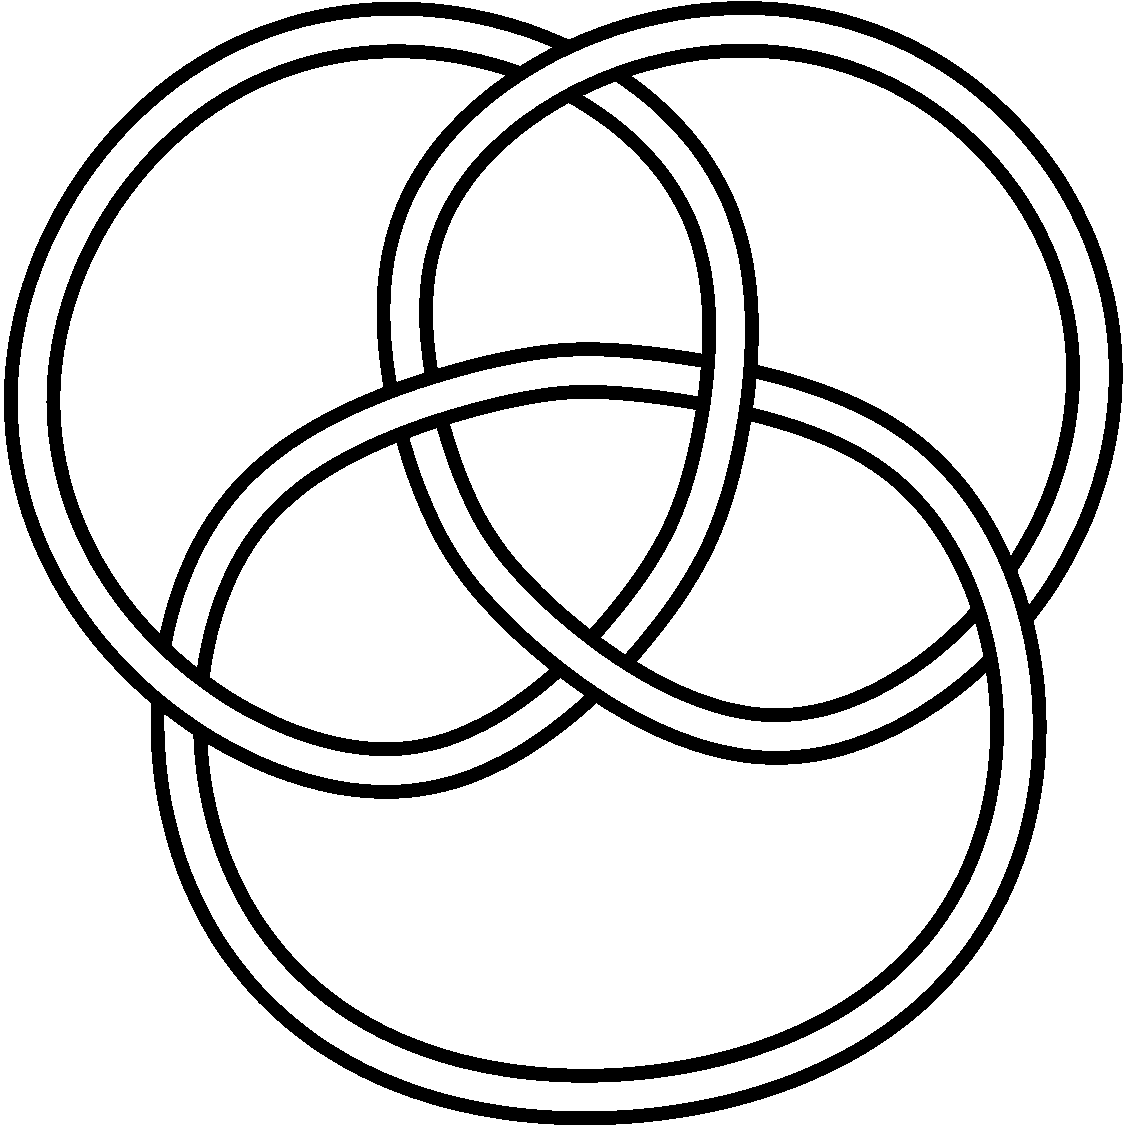
\includegraphics[scale=0.07,angle=0]{link6_2_3.pdf} 
& 
$
\displaystyle{%
\overline{\KR}_{2} = 2+\frac{q^4}{t^2}+\frac{t^2}{q^4}
}
$
\newline 
$
\displaystyle{%
\overline{\KR}_{3} = 3+\frac{1}{q^2}+q^2+\frac{q^4}{t^2}+\frac{q^6}{t^2}+\frac{t^2}{q^6}+\frac{t^2}{q^4}
}
$
\\
\hline
%%%%%%%%%%%%%%%%%%%%%%%%%%%%%%%%%%%%%%%%%%%%%%%%%%%%
$6_{2}^3\,\text{{\tiny (v2)}}$ 
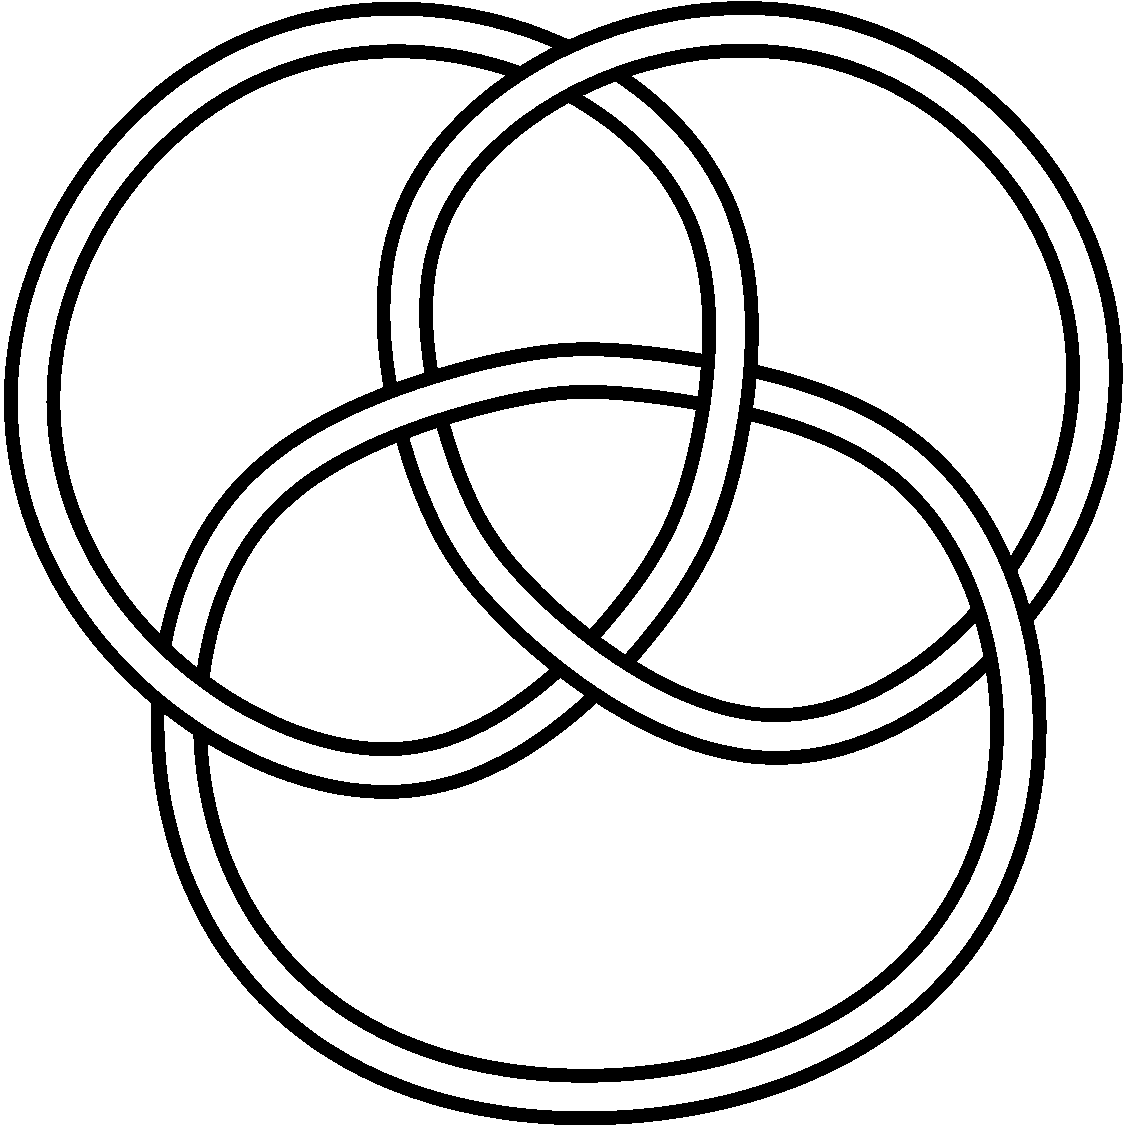
\includegraphics[scale=0.07,angle=0]{link6_2_3.pdf} 
& 
$
\displaystyle{%
\overline{\KR}_{2} = 4+\frac{q^6}{t^3}+\frac{3 q^4}{t^2}+\frac{2 q^2}{t}+\frac{2 t}{q^2}+\frac{3 t^2}{q^4}+\frac{t^3}{q^6}
}
$
\newline 
$
\displaystyle{%
\overline{\KR}_{3} = 5+\frac{2}{q^2}+2 q^2+\frac{q^8}{t^3}+\frac{q^4}{t^2}+\frac{2 q^6}{t^2}+\frac{2 q^2}{t}+\frac{2 t}{q^2}+\frac{2 t^2}{q^6}+\frac{t^2}{q^4}+\frac{t^3}{q^8}
}
$
\newline
$
\displaystyle{%
\overline{\KR}_{4} = 6+\frac{2}{q^4}+\frac{3}{q^2}+3 q^2+2 q^4+\frac{q^{10}}{t^3}+\frac{q^4}{t^2}+\frac{2 q^8}{t^2}+\frac{2 q^2}{t}+\frac{2 t}{q^2}+\frac{2 t^2}{q^8}+\frac{t^2}{q^4}+\frac{t^3}{q^{10}}
}
$
\\
\hline
%%%%%%%%%%%%%%%%%%%%%%%%%%%%%%%%%%%%%%%%%%%%%%%%%%%%
$6_{3}^2\,\text{{\tiny (v1)}}$ 

\includegraphics[scale=0.07,angle=0]{link6_3_2.pdf} 
& 
$
\displaystyle{%
2 q^{N-1}+\frac{q^{5 N-1}}{t^4}+\frac{q^{5 N+1}-q^{3 N+3}}{\left(q^2-1\right) t^4}+\frac{2 q^{3 N+1}}{t^3}+\frac{q^{N+3}}{t^2}+\frac{2 q^{3 N-1}}{t^2}+\frac{2 q^{N+1}}{t}+q^{1-N} t+q^{N-3} t+q^{-N-1} t^2
}
$
\newline\newline\newline\newline
Checked up to $N=3$. Extends result of~\cite{r0508510} to $N=3$. 
\\
\hline
%%%%%%%%%%%%%%%%%%%%%%%%%%%%%%%%%%%%%%%%%%%%%%%%%%%%
$6_{3}^2\,\text{{\tiny (v2)}}$ 

\includegraphics[scale=0.07,angle=0]{link6_3_2.pdf} 
& 
$
\displaystyle{%
q^{3-3 N}+q^{1-3 N} t+q^{3-5 N} t^2+2 q^{-3 N-1} t^2+2 q^{1-5 N} t^3+q^{-5 N-1} t^4-\frac{q^{-5 N-1} t^4}{q^2-1}+\frac{q^{-3 N-3} t^4}{q^2-1}+q^{1-7 N} t^5
}
$
\newline
$
\displaystyle{%
\qquad\qquad +q^{-5 N-3} t^5+q^{-7 N-1} t^6
}
$
\newline\newline\newline
Checked up to $N=3$. Extends result of~\cite{r0508510} to $N=3$. 
\\
\hline
%%%%%%%%%%%%%%%%%%%%%%%%%%%%%%%%%%%%%%%%%%%%%%%%%%%%
$6_{3}^3\,\text{{\tiny (v1)}}$
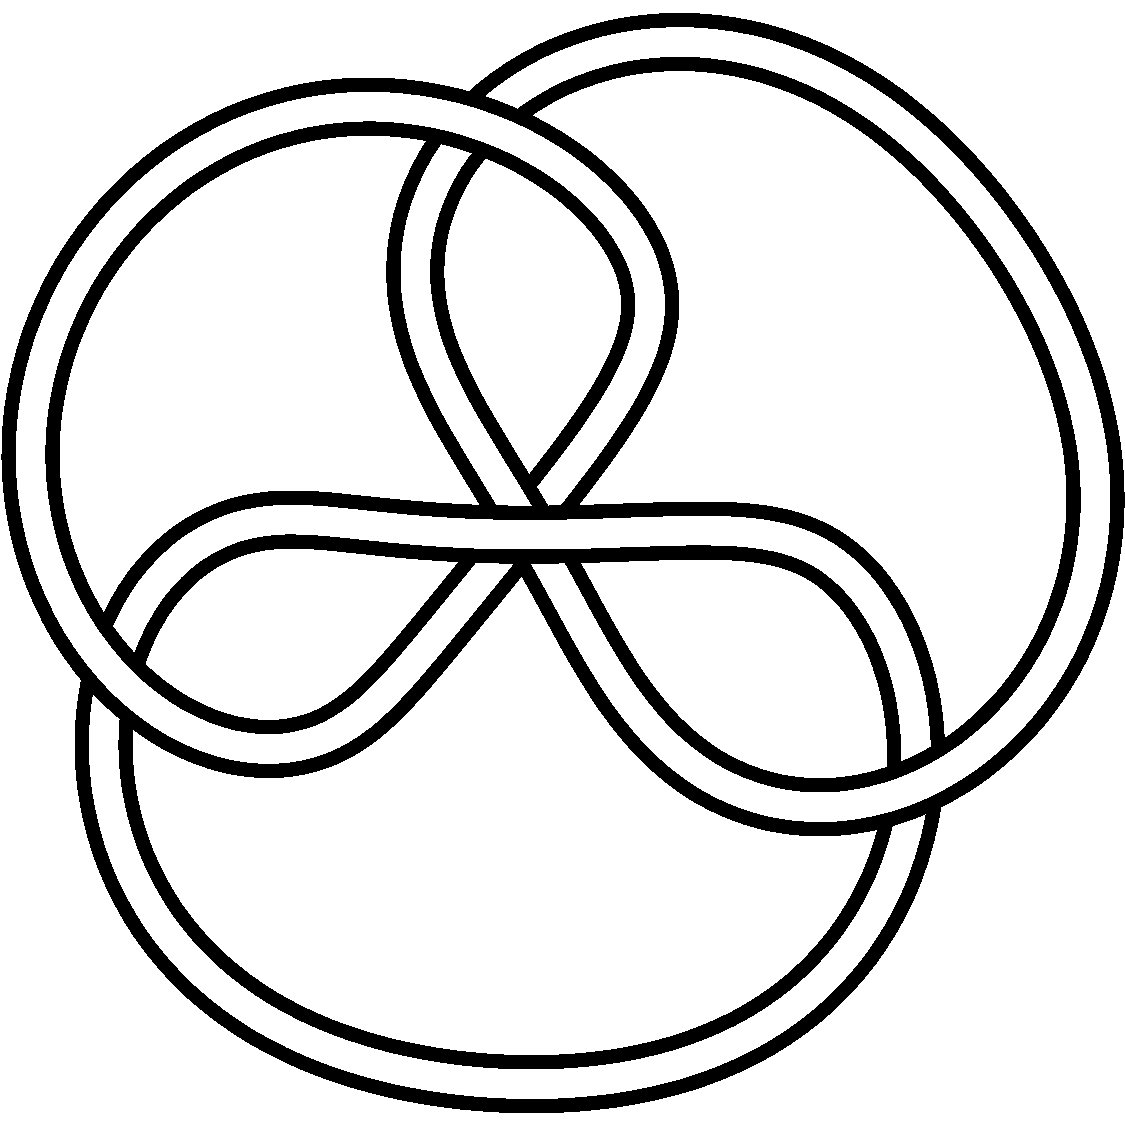
\includegraphics[scale=0.07,angle=0]{link6_3_3.pdf} 
& 
$
\displaystyle{%
\overline{\KR}_{2} = \frac{1}{q^4}+\frac{t^2}{q^8}+\frac{t^3}{q^{10}}+\frac{2 t^4}{q^{12}}+\frac{t^4}{q^{10}}
}
$
\newline 
$
\displaystyle{%
\overline{\KR}_{3} = \frac{1}{q^8}+\frac{t^2}{q^{12}}+\frac{t^3}{q^{16}}+\frac{2 t^4}{q^{18}}+\frac{3 t^4}{q^{16}}+\frac{t^4}{q^{14}}+\frac{t^6}{q^{22}}+\frac{t^6}{q^{20}}
}
$
\\
\hline
%%%%%%%%%%%%%%%%%%%%%%%%%%%%%%%%%%%%%%%%%%%%%%%%%%%%
$6_{3}^3\,\text{{\tiny (v2)}}$
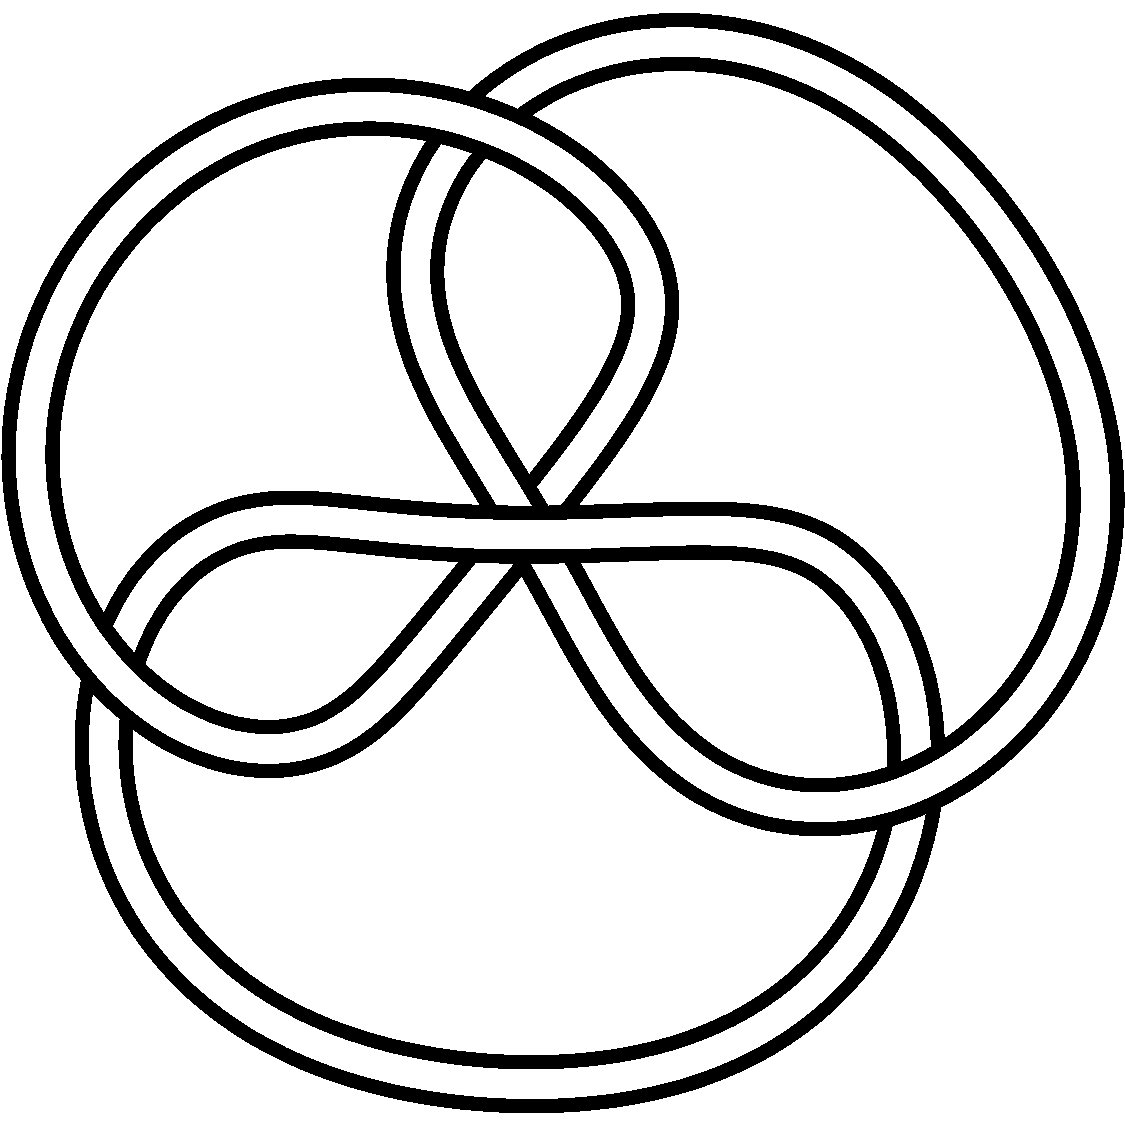
\includegraphics[scale=0.07,angle=0]{link6_3_3.pdf} 
& 
$
\displaystyle{%
\overline{\KR}_{2} = 2+q^2+\frac{q^8}{t^4}+\frac{q^4}{t^2}+\frac{q^2}{t}
}
$
\newline 
$
\displaystyle{%
\overline{\KR}_{3} = 2+2 q^2+q^4+\frac{q^{10}}{t^4}+\frac{q^{12}}{t^4}+\frac{2 q^6}{t^2}+\frac{q^8}{t^2}+\frac{q^2}{t}
}
$
\\
\hline
%%%%%%%%%%%%%%%%%%%%%%%%%%%%%%%%%%%%%%%%%%%%%%%%%%%%
\end{longtable}
}

%Notes to self:
%\begin{itemize}
%\item unreduced $7_{1}$ not included because we only have $N=2$
%\item unreduced $7_{1}^3$ not included because we only have $N=2$
%\item reduced $7_{1}$ not included because we only have $N\leqslant 3$
%\item reduced $7_{1}^3$ not included because we only have $N=2$
%\end{itemize}

\newpage
\appendix

\section{Properties of graded matrix factorisations}\label{appendix:graded_mfs}

\textbf{todo} Cite relevant places in KR.

Let $R = \bigoplus_{i \ge 0} R_i$ be a graded ring. If $X$ is a finite-rank graded matrix factorisation of $W \in R_{2c}$ over $R$ then the \emph{dual factorisation} is $X\mdual = \Hom_R(X,R)$, which factorises $-W$. More explicitly, the dual factorisation is the pair
\[
\xymatrix@C+3pc{
\Hom_R(X^0, R) \ar[r]^-{-\Hom(1, d^1_X)} & \Hom_R(X^1,R) \ar[r]^-{\Hom(1,d^0_X)} & \Hom_R(X^0, R) \, .
}
\]

\begin{remark}\label{remark:dual_koszul_cyclic} If $a,b \in R$ are homogeneous with $\deg(a) + \deg(b) = 2c$ then it is clear that there is an isomorphism $\{ b, a \}\mdual \cong \{-a, b\}$, and if we think of these cyclic Koszul factorisations as exterior algebras on a symbol $\theta$, this isomorphism sends the basis element $1^*$ to $1$ and $\theta^*$ to $\theta$.
\end{remark}

We will need the following basic facts relating the graded tensor and Hom. The proofs are easy (the standard isomorphisms for graded modules commute with the differentials) and we omit them.

\begin{lemma}\label{lemma:homdual} Given $W, W' \in R_{2c}$ and a finite-rank graded matrix factorisation $X$ of $W$ and a graded linear factorisation $Y$ of $W'$, there is a natural isomorphism
\[
\xi: X\mdual \otimes Y \lto \Hom_R(X,Y)
\]
of graded linear factorisations of $W' - W$, defined for $\Ztwo$-homogeneous elements $\nu \in X\mdual, y \in Y$ and $x \in X$ by $\xi( \nu \otimes y )(x) = (-1)^{|y||\nu|} \nu(x) \cdot y$.
\end{lemma}
% see NGMF

\begin{lemma} Given $X,Y,Z$ which are graded linear factorisations of $W, W', W'' \in R_{2c}$, respectively, there is a natural isomorphism of graded linear factorisations of $W'' - W' - W$
\[
\Hom_{\text{gr}}(X \otimes Y, Z) \lto \Hom_{\text{gr}}(X, \Hom_{\text{gr}}(Y,Z)) \, .
\]
\end{lemma}
% see NGMF

In particular if $X, Y$ are finite-rank graded matrix factorisations we have
\begin{equation}\label{eq:dual_tensor}
\begin{split}
(X \otimes Y)\mdual &= \Hom_R(X \otimes Y, R)\\
&\cong \Hom_R(X, \Hom_R(Y,R))\\
&\cong \Hom_R(X,R) \otimes \Hom_R(Y,R) = X\mdual \otimes Y\mdual.
\end{split}
\end{equation}
Finally, we want to fix our sign conventions for suspensions in the tensor product. The isomorphism $X\langle n \rangle \otimes Y \cong (X \otimes Y)\langle n \rangle$ involves no signs, but the isomorphism $X \otimes (Y \langle n \rangle) \cong (X \otimes Y)\langle n \rangle$ involves a sign $x \otimes y \longmapsto (-1)^{n|x|} x \otimes y$ for $\Ztwo$-homogeneous $x$. Grading shifts $\{ m \}$ can be pulled out of either component of a tensor product with no signs.
\\

In the following let $R = \bigoplus_{i \ge 0} R_i$ be a graded ring, and $\bs{a}, \bs{b}$ sequences of $n$ homogeneous elements in $R$ with $\deg(a_i) + \deg(b_i) = 2c$. If $\bs{a} = (a_1,\ldots,a_n)$ then $- \bs{a}$ denotes $(-a_1, \ldots, -a_n)$. In describing maps between cyclic Koszul complexes we use the symbols $\theta_i$ introduced in Subsection \ref{prelim:cyclic_koszul}.

\begin{lemma}\label{lemma:cyclickos1} There is a canonical isomorphism of graded matrix factorisations
\[
\{ \bs{a}, \bs{b} \}\mdual \cong \{ -\bs{b}, \bs{a} \} \, .
\]
\end{lemma}
\begin{proof}
Using Remark \ref{remark:dual_koszul_cyclic} we have
\begin{align*}
\{ \bs{a}, \bs{b} \}\mdual &\cong \left( \{ a_1, b_1 \} \otimes \ldots \otimes \{ a_n, b_n \} \right)\mdual\\
&\cong \{ a_1, b_1 \}\mdual \otimes \ldots \otimes \{ a_n, b_n \}\mdual\\
&\cong \{ -b_1, a_1 \} \otimes \ldots \otimes \{ -b_n, a_n \} = \{ - \bs{b}, \bs{a} \} \, .
\end{align*}
\end{proof}
% see ngkos

\begin{lemma}\label{lemma:cyclickos2} There is a canonical isomorphism of graded matrix factorisations
\begin{equation}
\label{abba}
\{ - \bs{a}, \bs{b} \} \cong \{ -\bs{b}, \bs{a} \}\langle n \rangle \Big\{ \sum_i \deg(a_i) - nc \Big\} \, .
\end{equation}
\end{lemma}
\begin{proof}
Let us begin with $a,b$ homogeneous such that $\deg(a) + \deg(b) = 2c$. Then $\{ a, b \}\langle 1 \rangle$ is
\[
\xymatrix{
R\{ \deg(a) - c \} \ar[r]^-{-a} & R \ar[r]^-{-b} & R\{ \deg(a) - c \}
}
\]
and shifting the grading by $\{ c - \deg(a) \}$ we have $\{ a, b \}\langle 1 \rangle\{ c - \deg(a) \}$ is equal to $\{ -b, -a \}$. Thus
\begin{align*}
\{ - \bs{a}, \bs{b} \} &\cong \{ -a_1, b_1 \} \otimes \ldots \otimes \{ -a_n, b_n \}\\
&\cong \{ -b_1, a_1 \}\langle 1 \rangle\{ \deg(a_1) - c \} \otimes \ldots \otimes \{ -b_n, a_n \}\langle 1 \rangle\{ \deg(a_n) - c \}\\
&\cong \{ -\bs{b}, \bs{a} \}\langle n \rangle\big\{ \sum_i \deg(a_i) - nc \big\}.
\end{align*}
\end{proof}

\begin{lemma}\label{lemma:cyclickos3} There is an isomorphism of graded matrix factorisations
\[
\{ \bs{a}, \bs{b} \} \cong \{ -\bs{a}, - \bs{b} \}\,,
\]
defined by $\theta_i \longmapsto - \theta_i$.
\end{lemma}

Finally, let us discuss the cohomology of cyclic Koszul complexes (\textbf{todo, fix}). Let $R$ be any ring. We begin more generally: let $C = \bigoplus_{i \in \mathds{Z}} C^i$ be a $\mathds{Z}$-graded $R$-module together with $R$-linear maps $d_{\pm}: C \lto C$ of degree $\pm 1$, satisfying
\[
(d_+)^2 = (d_{-})^2 = 0 \, , \qquad \text{and} \qquad d_{+}d_{-} + d_{-}d_{+} = 0 \, .
\]
Let $C_{\Ztwo}$ denote the $\Ztwo$-folding, which is a $\Ztwo$-graded complex with different $d_{\text{tot}} = d_+ + d_{-}$. If we replace $d_{+}$ by $-d_{+}$ then we have a second complex $(C_{\Ztwo}, -d_{+} + d_{-})$. We claim that these two complexes have the same $\Ztwo$-graded cohomology: this is the cyclic version of the obvious fact that multiplying the differentials on the ordinary Koszul complex by $-1$ does not change the cohomology. Recall that given a $\Ztwo$-graded complex $(X,d)$ we denote by $(X,d)_{-}$ the complex
\[
\xymatrix{%
X^0 \ar[r]^-{-d^0} & X^1 \ar[r]^-{d^1} & X^0\,.
}
\]

\begin{lemma}\label{lemma:cyclickoszulsign} There is a canonical isomorphism of $\Ztwo$-graded complexes
\[
T: (C_{\Ztwo}, d_{+} + d_{-}) \lto (C_{\Ztwo}, -d_{+} + d_{-})_{-}
\]
defined on $C^i$ by $T|_{C^i} = (-1)^{\frac{1}{2}i(i+1)}$. This induces an isomorphism
\[
H(C_{\Ztwo}, d_{+} + d_{-}) \lto H(C_{\Ztwo}, -d_{+} + d_{-}) \, .
\]
\end{lemma}
% see the note comfa

In particular for sequences $\bs{a}, \bs{b}$ we have
\begin{equation}
\label{Habba}
H(\{ \bs{a}, \bs{b} \}) \cong H(\{\bs{a}, -\bs{b}\}) \, .
\end{equation}

\section{The relation between reduced and unreduced homology}

As was discussed in Section~\ref{KRconstruction}, to a state graph $\Gamma$ with $m$ edges Khovanov and Rozansky assign a $\Ztwo$-graded complex $\krc(\Gamma)$ over the polynomial ring $R = \QQ[\boldsymbol{x}]$ in the edge variables $\boldsymbol{x} = \{x_1,\ldots,x_m\}$, defined by tensoring together local matrix factorisations assigned to the singular crossings and smoothings of the state graph. The definition depends on a choice of integer $N > 1$, which we fix throughout and omit from the notation, so that all our homologies are $\sln$ homologies.

The Khovanov-Rozansky complex $\krc(D)$ of a planar diagram $D$ of a link $L$ is defined by tensoring together two term complexes build from these $\krc(\Gamma)$'s, as $\Gamma$ varies over all resolutions of $D$, and recall that the unreduced and reduced Khovanov-Rozansky homology are defined respectively by
\begin{align*}
H(L) &= H\big( H(\krc(D),\diffm), \diffh \big) \, ,\\
\overline{H}(L, K) &= H\big( H( \krc(D) \otimes_{R} R/(x_i), \diffm), \diffh \big) \, ,
\end{align*}
where $K$ denotes a component of $L$, and $i$ is a label assigned in the planar diagram $D$ to an edge lying on this component. In this appendix we make some remarks about the relationship between reduced and unreduced homology. Let us fix the label $i$ in the following.

After taking the $\diffm$-cohomology everything becomes finite-dimensional, and taking the cohomology with respect to the differential $\diffh$ is straightforward; the whole problem with computing these invariants is computing $H(\krc(D), \diffm)$. In this article the emphasis is on computations, and in this context there is a big difference between taking cohomology before and after setting $x_i = 0$. Since $H(\krc(D), \diffm)$ is a direct sum of modules $H(\krc(\Gamma), \diffm)$ for various state graphs $\Gamma$ let us speak only of state graphs, in which case we are making the distinction between
\[
H(\krc(\Gamma) \otimes_R R/(x_i), \diffm ) \qquad \text{and} \qquad H( \krc(\Gamma), \diffm ) \otimes_R R/(x_i) \, .
\]
In the second case one computes the essential ingredient $H( \krc(\Gamma), \diffm )$ in the \emph{unreduced} homology, and then throws away information; in the first case one deals from the beginning with one less variable, so the computation is significantly easier. For this reason, the first definition (which is the original one of \cite{kr0401268}) is the one our code computes; but since the second definition is the one studied in \cite{r0607544} and other references, we want to explain the relationship between the two. Let us set
\begin{align*}
H(\Gamma) &= H( \krc(\Gamma), \diffm ) \, ,\\
\redh(\Gamma) &= H( \krc(\Gamma) \otimes_R R/(x_i), d ) \, .
\end{align*}
These are both finite-dimensional $(\mathds{Z} \times \Ztwo)$-graded vector spaces. It is shown in \cite{kr0401268} that $H(\Gamma)$ is concentrated in only one $\Ztwo$-degree, namely the degree of the parity $p = p(\Gamma)$ defined by erasing all wide edges in $\Gamma$ and counting the number of circles in the resulting link. It follows that the link homology $H(L)$, which is \emph{a priori} $(\ZZ \times \ZZ \times \Ztwo)$-graded, is actually only $(\ZZ \times \ZZ)$-graded.

On the other hand $\redh(\Gamma)$ has nonzero contributions in both $\Ztwo$-degrees, so the reduced link homology $\overline{H}(L,K)$, as defined in \cite{kr0401268}, is honestly $(\ZZ \times \ZZ \times \Ztwo)$-graded. We write $\redh^j(\Gamma)$, respectively $\redh^j(L,K)$, for the $\Ztwo$-component in degree $j \in \Ztwo$. The point of this appendix is to check that $\redh^0(L,K)$ and $\redh^1(L,K)$ only differ by a grading shift.

\begin{lemma}\label{lemma:redvsunred} There is an isomorphism of $(\ZZ \times \ZZ)$-graded $\mathds{Q}$-vector spaces 
\[
\redh^{p+1}(L,K) \cong \redh^{p}(L,K)\{N-1\} \, .
\]
\end{lemma}

This will follow if we can show that there is an isomorphism $\redh^{p+1}(\Gamma) \cong \redh^p(\Gamma)\{N-1\}$ natural with respect to the $\chi$ maps. It is easy to see that the two $\Ztwo$-components of $\redh(\Gamma)$ have the same dimension: it is the gradings that we need to compare. From the short exact sequence
\[
\xymatrix{%
0 \ar[r] & C(\Gamma) \ar[r]^-{x_{i}} & C(\Gamma)\{-2\} \ar[r] & C(\Gamma) \otimes_R R/(x)\{-2\} \ar[r] & 0
}
\]
we deduce a long exact sequence in cohomology, of graded $R$-modules:
\begin{equation}\label{eq:redvsunred_seq}
\xymatrix{%
0 \ar[r] & \redh^{p+1}(\Gamma)\{N-1\} \lto H(\Gamma) \ar[r]^-{x_{i}} & H(\Gamma)\{-2\} \ar[r] & \redh^p(\Gamma)\{-2\} \ar[r] & 0 \, ,
}
\end{equation}
It is clear from this exact sequence that the dimensions of the odd and even degrees of $\redh(\Gamma)$ agree (this is also observed in \cite[Proposition 3.12]{r0607544}). Moreover, assembling the $H(\Gamma)$'s to form the link homology, we deduce that
\[
\redh^p(L, K) \cong H(H(C(D),d) \otimes_R R/(x_i), d_{\chi})\,.
\]
As has already been mentioned, this $(\ZZ \times \ZZ)$-graded $\QQ$-vector space is adopted as the \emph{definition} of the reduced Khovanov-Rozansky homology in \cite{r0607544,websterblah, rasmussenblah}. In light of Lemma \ref{lemma:redvsunred} this is reasonable, as the other $\Ztwo$-degree of $\redh(L,K)$ contains no new information, but as far as we know the lemma has not appeared before in the literature (although it is no doubt known to the experts). To relate the $\ZZ$-gradings of $\redh^p(\Gamma)$ and $\redh^{p+1}(\Gamma)$ we make use of the following basic property of the space $H(\Gamma)$.

\textbf{Convention.} Since we ultimately only care about the homologies $H(L)$ and $\overline{H}(L,K)$, we are free to choose $D$ to be the closure of a braid with $i$ the label on one of the edges in the closure, and for the rest of this section we make this assumption. In particular, $\Gamma$ is a braid graph.

\begin{lemma}\label{lemma:directsumalgebras} $H(\Gamma)$ is concentrated in degree $p(\Gamma)$, and as a graded $\QQ[x_i]$-module it is isomorphic to a direct sum of copies of $\QQ[x_i]/(x_i^N)$ shifted in the $\mathds{Z}$-grading, that is, for some integers $b_j$ we have
\[
H(\Gamma) \cong \bigoplus_{j} \QQ[x_i]/(x_i^N)\{b_j\} \, .
\]
\end{lemma}

Further, one can prove that the integers $b_j$ have some symmetry: $H(\Gamma)$ is always self-dual as a graded vector space, but we will not need this. Taking the lemma as a given:

\begin{proof}[Proof of Lemma \ref{lemma:redvsunred}] We claim that $\redh^{p+1}(\Gamma) \cong \redh^p(\Gamma)\{N-1\}$ as graded vector spaces. In light of the exact sequence (\ref{eq:redvsunred_seq}), to understand $\overline{H}(\Gamma)$ it suffices to understand the action of $x_i$ on $H(\Gamma)$. But with Lemma \ref{lemma:directsumalgebras} in hand this is trivial: it reduces to understanding the action of $x_i$ on $\QQ[x_i]/(x_i^N)$, and we deduce that
\begin{align*}
\redh^{p+1}(\Gamma)\{N-1\} &\cong \bigoplus_j \QQ \cdot x_i^{N-1} \{ b_j \} = \bigoplus_j \QQ\{b_j + 2N - 2 \} \, ,\\
\redh^p(\Gamma) &\cong \bigoplus_j \QQ \{ b_j \}\,.
\end{align*}
From this we deduce that $\redh^{p+1}(\Gamma) \cong \bigoplus_j \QQ\{b_j + N - 1 \} \cong \redh^p(\Gamma)\{N-1\}$, as claimed.

Now suppose that $\Gamma, \Gamma'$ are state graphs of $D$ for which there is a morphism $\chi_k: C(\Gamma) \lto C(\Gamma')$. We need to prove that the diagram
\[
\xymatrix@C+1pc{
\redh^{p+1}(\Gamma) \ar[d]_{\redh^{p+1}\chi}\ar[r]^-{\cong} & \redh^p(\Gamma)\{N-1\}\ar[d]^{\redh^p \chi}\\
\redh^{p+1}(\Gamma') \ar[r]_-{\cong} & \redh^p(\Gamma')\{N-1\}
}
\]
commutes. Decompose $H(\Gamma), H(\Gamma')$ as in Lemma \ref{lemma:directsumalgebras} and let $\chi': \QQ[x_i]/(x_i^N) \lto \QQ[x_i]/(x_i^N)$ be one of the components of $\chi$. The corresponding component of $\redh^{p+1} \chi$ is the restriction of $\chi'$ to the ideal generated by $x_i^{N-1}$, and the component of $\redh^p \chi$ is the map induced by $\chi$ on the quotients by the ideal $(x_i)$. But since $\chi'$ is homogeneous it sends $1$ to $\lambda x_i^a$ for some $\lambda \in \QQ$ and $0 \le a \le N - 1$, and it is easy to see that if $a > 0$ then these components of $\redh^{p+1} \chi$ and $\redh^p \chi$ are both zero. On the other hand if $a = 0$ then the components are both multiplication by $\lambda$, and hence the diagram commutes. Since the differentials in $(H^p(C(D) \otimes_R R/(x_i),d), d_\chi)$ are built out of the $\chi$'s, we may conclude from this that $\redh^{p+1}(L,K) \cong \redh^{p}(L,K)\{N-1\}$, completing the proof.
\end{proof}

\begin{proof}[Proof of Lemma \ref{lemma:directsumalgebras}]
The argument is similar to that of \cite[Lemma 5.8]{r0607544}. We prove the claim by induction on the complexity of braid graphs $\Gamma$ together with a chosen edge $i$ appearing in the braid closure, using the induction scheme of Wu \cite{Wu} and the MOY relations~\eqref{MOYcatDecomp1}--\eqref{MOYcatDecomp4} proved in \cite[Section 6]{kr0401268}. Let us denote by $\Gamma_{\text{I}}, \Gamma_{\text{II}}, \Gamma_{\text{III}}$ the graphs which are the arguments of~$C$ on the left of \eqref{MOYcatDecomp1}, \eqref{MOYcatDecomp2}, \eqref{MOYcatDecomp4}, respectively. 

By \cite{Wu}, if $\Gamma$ is the closure of an open braid graph $\Gamma_{\text{open}}$ then $\Gamma$ always contains a region of the form $\Gamma_{\text{I}}$, or $\Gamma_{\text{open}}$ contains a region $\Gamma_{\text{II}}$ or $\Gamma_{\text{III}}$. This means that using only the MOY relations we can go from any braid graph to a family of unlinked circles, and in this base case $H(\Gamma)$ is a tensor product over $\mathds{Q}$ of grading shifted copies of $\QQ[x_j]/(x_j^N)\langle 1 \rangle$ for various $j$. By hypothesis $i$ is among these indices, so both claims are clear in the base case.

The only MOY relation which changes the parity is relation~\eqref{MOYcatDecomp1}, which changes the parity by one and also introduces a suspension, so it is now clear by induction that $H(\Gamma)$ is always concentrated in degree $p(\Gamma)$, and we need to check the other claim.

Given a braid graph $\Gamma$ suppose that we can find a region of type $\Gamma_{\text{II}}$ or $\Gamma_{\text{III}}$ in $\Gamma_{\text{open}}$. Then the corresponding direct sum decomposition has $x_i$ as an external variable, so the equivalences of the decompositions are $x_i$-linear. By the inductive hypothesis the cohomology of all the other braid graphs involved in the decomposition are direct sums of grading shifted copies of $\QQ[x_i]/(x_i^N)$ so the same is true of $C(\Gamma)$.

It remains to treat the case where we can only find a region of type $\Gamma_{\text{I}}$, the catch being that $x_i$ may not be an external variable to the decomposition: $i$ may be the loop contracted away by the MOY relation. But in this case we may assume that, apart from some circles which we may ignore, the edge $i$ is the rightmost edge in the braid graph. 

In this situation we consider the dual braid graph $\Gamma^{\lor}$ where we reverse the orientation of all the edges. Note that for some sequences of polynomials $\boldsymbol{a},\boldsymbol{b}$ and an integer $c$ we have $C(\Gamma) = \{ \boldsymbol{a}, \boldsymbol{b} \}\{c\}$, and using~\eqref{abba} it follows that
\[
C(\Gamma^{\lor}) = C(\Gamma)\mdual = \{ \boldsymbol{a}, \boldsymbol{b} \}\{c\}\mdual \cong \{ \bs{a}, -\bs{b} \}\{ \sum_i \deg(a_i) - m(N+1) - c \}\,.
\]
But by~\eqref{Habba} $\{ \bs{a}, -\bs{b} \}$ has the same cohomology as $\{ \bs{a}, \bs{b} \}$, so up to grading shifts the cohomology of $\Gamma$ and $\Gamma^{\lor}$ agree. It therefore suffices to prove the claim for $\Gamma^{\lor}$. This follows by the above argument, since $i$ is the leftmost edge and can therefore never be involved in a $\Gamma_{\text{I}}$-relation.
\end{proof}

\section{Stabilisation}\label{section:morphismpert}
% dcct, skrh, ptons

In this appendix we use perturbation techniques to study stabilisation. For simplicity graded matrix factorisations will not feature here: this means that we work throughout with matrix factorisations in the usual sense. One nonstandard piece of terminology is that for us a \emph{linear factorisation} of~$W \in R$ is an arbitrary $\Ztwo$-graded $R$-module with an odd differential squaring to multiplication by $W$. One can tensor and Hom such things in the obvious way; see for example \cite[Section 2]{dm1102.2957}.

Let $R$ be a noetherian ring and take sequences $\ba = (a_1,\ldots,a_n)$ and $\bb = (b_1, \ldots, b_n)$ in $R$ with~$\bs{b}$ regular, and set $W = \sum_i a_i b_i$. We define the matrix factorisation $\{ \ba, \bb \}$ of $W$ as in Subsection \ref{prelim:cyclic_koszul} so $F = \bigoplus_i R \theta_1$ with $|\theta_i| = -1$ and $\bigwedge F$ has two differentials $\delta_+$ and $\delta_{-}$ such that $\{ \ba, \bb \} = (\bigwedge F, \delta_+ + \delta_{-})$. If we use only the differential $\delta_+$ then this is just the Koszul complex on the $b_i$, so there is a morphism of complexes from the Koszul complex to its cohomology
\begin{equation}\label{eq:app_stab0}
\pi: ( \bigwedge F, \delta_+ ) \lto R/(\bb)\,.
\end{equation}
In fact the map $\pi$ commutes with $\delta_{-}$, so $\pi$ is also morphism of linear factorisations $\{ \ba, \bb \} \lto R/(\bb)$. The task we give ourselves is to show that under some mild hypotheses this map is universal, in the following sense: for any finite-rank matrix factorisation $Y$ of $W$ we claim that the map
\begin{equation}\label{eq:app_stab1}
\Hom(1, \pi): \Hom_R(Y, \{ \ba, \bb \}) \lto \Hom_R(Y, R/(\bb))
\end{equation}
is a quasi-isomorphism. That is, $\{ \ba, \bb \}$ \emph{stabilises} $R/(\bb)$. This is a standard fact \cite{tobythesis,eisenbud} but the twist here is that we produce an explicit homotopy inverse. The first step is to use (the ungraded analogue of) Lemma \ref{lemma:homdual} to rewrite (\ref{eq:app_stab1}) up to isomorphism as
\begin{equation}\label{eq:app_stab2}
1 \otimes \pi: Y\mdual \otimes \{ \ba, \bb \} \lto Y \mdual \otimes R/(\bb).
\end{equation}
Our starting point is the fact that, turning off the differential $\delta_-$, $(Y\mdual \otimes \bigwedge F, \delta_+)$ is a direct sum of copies of the Koszul complex on the $b_i$, and is therefore quasi-isomorphic to $(Y\mdual \otimes R/(\bb), 0)$. If over some smaller ring (say $R$ contains a field) this is actually a homotopy equivalence, then using the language of deformation retracts and perturbation we can promote an inverse for this homotopy equivalence to an inverse for (\ref{eq:app_stab2}). Rather than repeat the basic facts about perturbation here, we direct the reader to \cite[Section 5]{dm1102.2957} for a full discussion; from now on we use the notation of \emph{loc.\,cit.}

Suppose that $R$ is an algebra over a ring $S$ and that the map $\pi$ in (\ref{eq:app_stab0}) is a homotopy equivalence of $\ZZ$-graded complexes over $S$. More specifically, suppose that there is an $S$-linear morphism of complexes $\sigma: R/(\bb) \lto (\bigwedge F, \delta_+)$ and an $S$-linear homotopy $h$ on $\bigwedge F$ such that $\delta_+ h + h \delta_+ = 1 - \sigma \pi$, $h^2 = 0$ and $h \sigma = 0$. In a moment we will explain how to produce such homotopies, using connections.

With $Y$ as above, there is a a deformation retract of linear factorisations of zero over $S$
\begin{equation}\label{eq:pre_perturb_htm3}
\xymatrix@C+2pc{
(Y\mdual \otimes R/(\bb), 0) \ar@<-0.8ex>[r]_{1 \otimes \sigma} & (Y\mdual \otimes \bigwedge F, 1 \otimes \delta_+), \ar@<-0.8ex>[l]_{\pi}
} \quad - 1 \otimes h \, .
\end{equation}
Here we fix a homogeneous basis for $Y$, and therefore for $Y\mdual$, and use it to extend $h, \sigma$ to $S$-linear maps on the tensor products (using Koszul signs in the case of $h$, which has degree one). Then the conditions for a deformation retract are simply a restatement of our hypothesis on $\sigma, h$ and $\pi$. 

Next we view $\mu = d_{Y\mdual} \otimes 1 + 1 \otimes \delta_{-}$ as a perturbation on $Y\mdual \otimes \bigwedge F$. The total differential $1 \otimes \delta_+ + \mu$ is the usual differential on the tensor product $Y\mdual \otimes \{ \ba, \bb \}$, and the perturbation lemma furnishes us with another deformation retract of $\Ztwo$-graded complexes over $S$
\[
\xymatrix@C+2pc{
(Y\mdual \otimes R/(\bb), d_{Y\mdual}\otimes 1) \ar@<-0.8ex>[r]_-{\sigma_\infty} & (Y\mdual \otimes \bigwedge F, 1 \otimes \delta_+ + \mu), \ar@<-0.8ex>[l]_-{1 \otimes \pi}
} \quad h_\infty
\]
here $h_\infty$ is a homotopy whose exact form does not concern us, and $\sigma_\infty = \sum_{m \ge 0} (-1)^m (h \mu)^m \sigma$. In particular $1 \otimes \pi$ is a homotopy equivalence over $S$, and thus from the commutative diagram
\begin{equation}\label{eq:cons3}
\xymatrix@C+2pc{
\Hom_R(Y, \{\ba, \bb\}) \ar[r]^-{\Hom(1,\pi)} & \Hom_R(Y, R/(\bb))\\
Y^{\lor} \otimes \{ \ba, \bb \} \ar[u]^{\cong} \ar[r]_-{1 \otimes \pi} & Y^{\lor} \otimes R/(\bb) \ar@/^2pc/[l]^-{\sigma_\infty} \ar[u]_{\cong}
}
\end{equation}
we learn that $\Hom(1,\pi)$ is a homotopy equivalence over $S$ (and hence a quasi-isomorphism over $R$, as claimed) and moreover we have a homotopy inverse $\sigma_\infty$. To actually use $\sigma_\infty$ to lift morphisms $Y \lto R/(\bb)$ to morphisms $Y \lto \{ \ba, \bb \}$, we need a concrete homotopy $h$. Let us turn to this now.

Rather than proceed in complete generality, let us specialise to situation of Subsection \ref{section:stabilisation}, where $S = \QQ[x_1, x_2], R = \QQ[x_1,x_2,y_1,y_2]$ and $W = y_1^{N+1} + y_2^{N+1} - x_1^{N+1} - x_2^{N+1}$. The cyclic Koszul complex of interest is $\Xcirc = \{ \ba, \bs{t} \}$, where $t_i = y_i - x_i$ and the sequence $\ba = (a_1,a_2)$ is the one elaborated in Subsection \ref{section:stabilisation}. This means that we take $\bb = \bs{t}$ in the above. 

Since we are interested in morphisms $\Xbul \lto \Xcirc$, in addition we take $Y = \Xbul$. We can write $R$ as $S[t_1,t_2]$ so there is an $S$-linear standard (in the sense of \cite[Section 8.1]{dm1102.2957}) flat connection
\begin{gather*}
\nabla: R \lto R \otimes_{S[\boldsymbol{t}]} \Omega^1_{S[\boldsymbol{t}]/S} \, ,\\
\nabla( f(x_1,x_2,y_1,y_2) ) = \frac{\partial f}{\partial y_1} \ud t_1 + \frac{\partial f}{\partial y_2} \ud t_2 \, .
\end{gather*}
This induces an $S$-linear map, also denoted $\nabla$, on $R \otimes_{S[\boldsymbol{t}]} \Omega_{S[\boldsymbol{t}]/S}$ where $\Omega = \bigwedge^\bullet \Omega^1$. We identify this free $\mathds{Z}$-graded $R$-module with $\bigwedge F$ via $\ud t_i = \theta_i$. It is easily checked that for $\theta = \theta_{i_1} \ldots \theta_{i_p}$ with distinct indices $i_j$ and $p > 0, f \in R$,
\[
(\nabla \delta_+ + \delta_+ \nabla)(f \cdot \theta) = (p + \delta_{+}\nabla)(f) \cdot \theta \, ,
\]
and moreover the $S$-linear operator $p \cdot 1_R + \delta_{+} \nabla$ on $R$ is invertible. It will be convenient to have notation for the inverse operator on $R$.

\begin{definition}\label{defn:omega} For $p > 0$ we write $\Omega_p = (p \cdot 1_R + \delta_{+} \nabla)^{-1}$. So by definition $\Omega_p(f)$ is the unique polynomial solution of the partial differential equation in an unknown $z$,
\[
p z + \frac{\partial z}{\partial y_1} (y_1 - x_1) + \frac{\partial z}{\partial y_2}(y_2 - x_2) = f \, .
\]
\end{definition}

\begin{example}\label{example:compomega} For a monomial $f = x_1^{c_1} x_2^{c_2} t_1^{d_1} t_2^{d_2}$ we have by direct computation $\Omega_p(f) = \frac{1}{p + d_1 + d_2} f$. Hence in particular
\begin{itemize}
\item[(i)] If $f \in k[x_1,x_2]$ then $\Omega_p(f) = \frac{1}{p} f$,
\item[(ii)] $\Omega_p(y_i) = \Omega_p(x_i + t_i) = \frac{1}{p(p+1)} x_i + \frac{1}{p+1} y_i$.
\end{itemize}
\end{example}

One defines a degree $-1$ $S$-linear map
\[
H = (\nabla \delta_+ + \delta_+ \nabla)^{-1} \nabla
\]
on the module $\bigwedge F$. Each application of $H$ involves differentiation with respect to the $y_i$, and then solving a differential equation. Let $\sigma: S = R/(\boldsymbol{t}) \lto \bigwedge F$ be the inclusion of $\QQ[x_1,x_2]$ into $R$. One checks (see \cite[Section 8.1]{dm1102.2957}) that $H \delta_+ + \delta_+ H = 1 - \sigma \pi$, so that $\sigma$ is exhibited by $H$ as the $S$-linear homotopy inverse to the morphism $\pi: (\bigwedge F, \delta_+) \lto (R/(\boldsymbol{t}),0)$.

As explained above, we tensor with $Y\mdual$ and perturb in the other differentials. The first step is to extend $H$ and $\sigma$ to $S$-linear maps
\[
\xymatrix@C+2pc{
Y\mdual \otimes \bigwedge F \ar@(dl,dr)[]_{H} & Y\mdual \otimes R/(\boldsymbol{t}) \ar[l]_{\sigma}
}
\]
using the homogeneous basis $1^*, \theta_1^*, \theta_2^*, (\theta_1\theta_2)^*$ for $Y\mdual$. This involves Koszul signs as we move~$H$ and~$\sigma$ past homogeneous elements of $X^{\lor}$, for example, $H(\theta_1^* \otimes f \theta_2) = - \theta_1^* \otimes H(f \theta_2)$. 

Next we consider the $R$-linear map
\[
\mu = d_{Y\mdual} \otimes 1 + 1 \otimes \delta_{-}
\]
on $Y\mdual \otimes \bigwedge F$, viewed as a perturbation of the differential on $(Y\mdual \otimes \bigwedge, 1 \otimes \delta_{+})$. The total differential $\mu + 1 \otimes \delta_{+}$ is the usual differential on the tensor product, and the perturbation lemma tells us that the $S$-linear map $\sigma_\infty = \sum_{m \ge 0} (-1)^m (H \mu)^m \sigma$ is an $S$-homotopy inverse to $1 \otimes \pi$. Composing with the vertical isomorphisms in (\ref{eq:cons3}) we have the desired inverse of $\Hom(1,\pi)$. The morphism (\ref{eq:cons4}) corresponds to the tensor $1^* \otimes 1 \in Y\mdual \otimes R/(\boldsymbol{t})$, so to find $\chi_1$ we are left with the task of evaluating
\[
\sigma_\infty(1^* \otimes 1) = \sigma(1^* \otimes 1) - H \mu \sigma(1^* \otimes 1) + H \mu H \mu(1^* \otimes 1) \, .
\]

\begin{proof}[Proof of Lemma \ref{lemma:consfirst}]
The map corresponding to $\sigma_\infty(1^* \otimes 1)$ makes (\ref{eq:cons5}) commute, so we need to evaluate this tensor and show that it has the explicit form given in the statement of the lemma. The notation becomes a little involved: throughout recall that we are producing tensors in $Y\mdual \otimes \bigwedge F$, an $R$-basis of which is given by tensors $\theta_1^* \otimes 1, 1^* \otimes \theta_1\theta_2$, etc. Clearly $\sigma(1^* \otimes 1)$ is just $1^* \otimes 1$, and
% compared to skrh we use s_i instead of d_i, and pi_i instead of a_i
\begin{align*}
H \mu \sigma(1^* \otimes 1) &= H( d_{X^{\lor}} + \delta_{-})(1^* \otimes 1)\\
&= H( -\theta_1^* \otimes s_1 - \theta_2^* \otimes s_2 + 1^* \otimes \pi_1 \theta_1 + 1^* \otimes \pi_2 \theta_2 )\\
&= \theta_1^* \otimes H(s_1) + \theta_2^* \otimes H(s_2) + 1^* \otimes H(\pi_1 \theta_1) + 1^* \otimes H(\pi_2 \theta_2) \, .
\end{align*}
By easy computations, for example
\begin{align*}
H(s_1) &= \Omega_1\Big( \frac{\partial s_1}{\partial y_1} \Big) \theta_1 + \Omega_1\Big( \frac{\partial s_1}{\partial y_2} \Big) \theta_2 = \Omega_1(1) \theta_1 + \Omega_1(1) \theta_2 = \theta_1 + \theta_2 \, ,
\end{align*}
and
\begin{align*}
H(\pi_1 \theta_1) &= (\nabla \delta_{+} + \delta_{+} \nabla)^{-1} \nabla( \pi_1 \theta_1 ) = (\nabla \delta_{+} + \delta_{+} \nabla)^{-1}\Big( \frac{\partial \pi_1}{\partial y_2} \theta_2 \theta_1 \Big) = 0 \, ,
\end{align*}
we find that
\begin{equation}\label{eq:cons6}
H \mu \sigma(1^* \otimes 1) = \theta_1^* \otimes (\theta_1 + \theta_2) + \frac{1}{2}\theta_2^* \otimes ( (x_2 + y_2) \theta_1 + (x_1 + y_1) \theta_2) \, .
\end{equation}
Applying $H\mu$ again we obtain after some work an expression for $H\mu H\mu\sigma(1^* \otimes 1)$, which we combine with the previous equation to find
\begin{equation}\label{eq:cons7}
\begin{split}
\sigma_\infty(1^* \otimes 1) &= 1^* \otimes 1 + 1^* \otimes \Omega_2\Big( \frac{\partial u_1}{\partial y_1} - \frac{\partial u_1}{\partial y_2} - \frac{1}{2} \frac{\partial u_2}{\partial y_2}(x_2 + y_2) + \frac{1}{2} \frac{\partial u_2}{\partial y_1}(x_1 + y_1) \Big)\theta_1 \theta_2\\
& \qquad+  \frac{1}{2}(\theta_1 \theta_2)^* \otimes (x_1 + y_1 - x_2 - y_2) \theta_1 \theta_2\\
& \qquad- \theta_1^* \otimes (\theta_1 + \theta_2) - \frac{1}{2} \theta_2^* \otimes ( (x_2+y_2)\theta_1 + (x_1+y_1)\theta_2 ) \, .
\end{split}
\end{equation}
The image under the canonical isomorphism $\xi: \Xbul\mdual \otimes \Xcirc \lto \Hom_R(\Xbul, \Xcirc)$ is our morphism $\chi_1 := \xi \sigma_\infty(1^* \otimes 1)$, which has the desired form (the signs get corrected by Koszul signs in $\xi$).
\end{proof}


\newcommand{\etalchar}[1]{$^{#1}$}
\providecommand{\href}[2]{#2}
\begin{thebibliography}{FYH{\etalchar{+}}85}

\bibitem[AS]{as1105.5117}
M.~Aganagic and S.~Shakirov, \emph{Knot {H}omology from {R}efined
  {C}hern-{S}imons {T}heory},
  \href{http://arxiv.org/abs/1105.5117}{[arXiv:1105.5117]}.

\bibitem[BN03]{bnKhovanov11crossings}
D.~Bar-Natan, \emph{Khovanov {H}omology for {K}nots and {L}inks with up to 11
  {C}rossings}, available at
  \href{http://www.math.toronto.edu/drorbn/papers/KHTables/KHTables.pdf}{http:%
//www.math.toronto.edu/drorbn/papers/KHTables/KHTables.pdf}.

\bibitem[BR07]{br0707.0922}
I.~Brunner and D.~Roggenkamp, \emph{B-type defects in {L}andau-{G}inzburg
  models}, JHEP \textbf{0708} (2007), 093,
  \href{http://arxiv.org/abs/0707.0922}{[arXiv:0707.0922]}.

\bibitem[CF94]{cf9405183}
L.~Crane and I.~B. Frenkel, \emph{Four dimensional topological quantum field
  theory, {H}opf categories, and the canonical bases}, J. Math. Phys.
  \textbf{35} (1994), 5136--5154,
  \href{http://arxiv.org/abs/hep-th/9405183}{[hep-th/9405183]}.

\bibitem[CK08a]{ck0701194}
S.~Cautis and J.~Kamnitzer, \emph{Knot homology via derived categories of
  coherent sheaves {I}, {$sl(2)$} case}, Duke Math. J. \textbf{142} (2008),
  511--588, \href{http://arxiv.org/abs/math/0701194}{[math.AG/0701194]}.

\bibitem[CK08b]{ck0710.3216}
S.~Cautis and J.~Kamnitzer, \emph{Knot homology via derived categories of coherent sheaves {II},
  {$sl(m)$} case}, Invent. Math. \textbf{174} (2008), 165--232,
  \href{http://arxiv.org/abs/math/0710.3216}{[math.AG/0710.3216]}.

\bibitem[CM]{cmWebCompileCode}
N.~Carqueville and D.~Murfet, \emph{Code to compute {K}hovanov-{R}ozansky
  homology and defect fusion in {L}andau-{G}inzburg models},
  \href{http://www.carqueville.net/nils/webCompilations}{http://www.carqueville.net/nils/webCompilations}.

\bibitem[CR]{cr1006.5609}
N.~Carqueville and I.~Runkel, \emph{Rigidity and defect actions in
  landau-ginzburg models},
  \href{http://arxiv.org/abs/1006.5609}{[arXiv:1006.5609]}.

\bibitem[CR10]{cr0909.4381}
N.~Carqueville and I.~Runkel, \emph{On the monoidal structure of matrix bi-factorisations}, J. Phys.
  A: Math. Theor. \textbf{43} (2010), 275401,
  \href{http://arxiv.org/abs/0909.4381}{[arXiv:0909.4381]}.

\bibitem[DGR06]{dgr0505662}
N.~M. Dunfield, S.~Gukov, and J.~Rasmussen, \emph{The {S}uperpolynomial for
  {K}not {H}omologies}, Experimental Math. \textbf{15} (2006), 129--159,
  \href{http://arxiv.org/abs/math/0505662}{[math.GT/0505662]}.

\bibitem[DKR]{dkr1107.0495}
A.~Davydov, L.~Kong, and I.~Runkel, \emph{Field theories with defects and the
  centre functor}, \href{http://arxiv.org/abs/1107.0495}{[arXiv:1107.0495]}.

\bibitem[DM]{dm1102.2957}
T.~Dyckerhoff and D.~Murfet, \emph{Pushing forward matrix factorisations},
  \href{http://arxiv.org/abs/1102.2957}{[arXiv:1102.2957]}.

\bibitem[FFRS07]{ffrs0607247}
J.~Fr\"ohlich, J.~Fuchs, I.~Runkel, and C.~Schweigert, \emph{Duality and
  defects in rational conformal field theory}, Nucl. Phys. B \textbf{763}
  (2007), 354--430,
  \href{http://arxiv.org/abs/hep-th/0607247}{[hep-th/0607247]}.

\bibitem[FYH{\etalchar{+}}85]{Homfly}
P.~Freyd, D.~Yetter, J.~Hoste, W.~B.~R. Lickorish, K.~Millett, and A.~Ocneanu,
  \emph{A new polynomial invariant of knots and links}, Bull. Amer. Math. Soc.
  \textbf{12} (1985), 239--246.

\bibitem[GIKV10]{gikv0705.1368}
S.~Gukov, A.~Iqbal, C.~Koz\c{c}az, and C.~Vafa, \emph{Link {H}omologies and the
  {R}efined {T}opological {V}ertex}, Commun. Math. Phys. \textbf{298} (2010),
  757--785, \href{http://arxiv.org/abs/0705.1368}{[arXiv:0705.1368]}.

\bibitem[GSV05]{gsv0412243}
S.~Gukov, A.~Schwarz, and C.~Vafa, \emph{Khovanov-{R}ozansky {H}omology and
  {T}opological {S}trings}, Lett. Math. Phys. \textbf{74} (2005), 53--74,
  \href{http://arxiv.org/abs/hep-th/0412243}{[hep-th/0412243]}.

\bibitem[GV99]{gv9811131}
R.~Gopakumar and C.~Vafa, \emph{On the {G}auge {T}heory/{G}eometry
  {C}orrespondence}, Adv. Theor. Math. Phys. \textbf{3} (1999), 1415--1443,
  \href{http://arxiv.org/abs/hep-th/9811131}{[hep-th/9811131]}.

\bibitem[GW]{gw0512298}
S.~Gukov and J.~Walcher, \emph{Matrix {F}actorizations and {K}auffman
  {H}omology}, \href{http://arxiv.org/abs/hep-th/0512298}{[hep-th/0512298]}.

\bibitem[Jae]{j1101.3302}
T.~C. Jaeger, \emph{Khovanov-{R}ozansky {H}omology and {C}onway {M}utation},
  \href{http://arxiv.org/abs/1101.3302}{[arXiv:1101.3302]}.

\bibitem[Jon85]{JonesPolynomialPaper}
V.~F.~R. Jones, \emph{A polynomial invariant for knots via von {N}eumann
  algebras}, Bull. Amer. Math. Soc. \textbf{12} (1985), 103--111.

\bibitem[Kap]{k1004.2307}
A.~Kapustin, \emph{Topological {F}ield {T}heory, {H}igher {C}ategories, and
  {T}heir {A}pplications},
  \href{http://arxiv.org/abs/1004.2307}{[arXiv:1004.2307]}.

\bibitem[Kaw96]{kawauchibook}
A.~Kawauchi, \emph{A {S}urvey of {K}not {T}heory}, Birkh\"auser, 1996.

\bibitem[Kho00]{k9908171}
M.~Khovanov, \emph{A categorification of the {J}ones polynomial}, Duke Math. J.
  \textbf{101} (2000), 359--426,
  \href{http://arxiv.org/abs/math/9908171}{[math.QA/9908171]}.

\bibitem[KR07]{kr0701333}
M.~Khovanov and L.~Rozansky, \emph{Virtual crossings, convolutions and a
  categorification of the {$\operatorname{SO}(2N)$} {K}auffman polynomial},
  Journal of G\"okova Geometry Topology \textbf{1} (2007), 116--214,
  \href{http://arxiv.org/abs/math/0701333}{[math.QA/0701333]}.

\bibitem[KR08a]{kr0401268}
M.~Khovanov and L.~Rozansky, \emph{Matrix factorizations and link homology}, Fund. Math.
  \textbf{199} (2008), 1--91,
  \href{http://arxiv.org/abs/math/0401268}{[math/0401268]}.

\bibitem[KR08b]{kr0505056}
M.~Khovanov and L.~Rozansky, \emph{Matrix factorizations and link homology {II}}, Geometry \&
  Topology \textbf{12} (2008), 1387--1425,
  \href{http://arxiv.org/abs/math/0505056}{[math.QA/0505056]}.

\bibitem[Lam86]{LambekRingsModules}
J.~Lambek, \emph{Lectures on rings and modules}, AMS Chelsea Publishing, 1986.

\bibitem[LM]{Calinetal2}
C.~I. Lazaroiu and D.~McNamee, unpublished.

\bibitem[LMnV00]{lmv0010102}
J.~M.~F. Labastida, M.~Mari\~{n}o, and C.~Vafa, \emph{Knot {I}nvariants and
  {T}opological {S}trings}, JHEP \textbf{0011} (2000), 007,
  \href{http://arxiv.org/abs/hep-th/0010102}{[hep-th/0010102]}.

\bibitem[Man07]{m0601629}
C.~Manolescu, \emph{Link homology theories from symplectic geometry}, Adv. in
  Math. \textbf{211} (2007), 363--416,
  \href{http://www.arxiv.org/abs/math.AG/0601629}{[math.SG/0601629]}.

\bibitem[McN]{McNameethesis}
D.~McNamee, \emph{On the mathematical structure of topological defects in
  {L}andau-{G}inzburg models}, MSc Thesis, Trinity College Dublin, 2009.

\bibitem[Mn05]{marinoknotbook}
M.~Mari\~{n}o, \emph{Chern-{S}imons {T}heory, {M}atrix {M}odels, and
  {T}opological s{t}rings}, Oxford University Press, 2005.

\bibitem[MOY98]{moy1998}
H.~Murakami, T.~Ohtsuki, and S.~Yamada, \emph{Homfly polynomial via an
  invariant of colored plane graphs}, Enseign. Math. \textbf{44} (1998),
  325--360.

\bibitem[MS]{ms0709.1971}
V.~Manzorchuck and C.~Stroppel, \emph{A combinatorial approach to functorial
  quantum {$\mathfrak{sl}_k$} knot invariants},
  \href{http://arxiv.org/abs/0709.1971}{[arXiv:0709.1971]}.

\bibitem[OV00]{ov9912123}
H.~Ooguri and C.~Vafa, \emph{Knot {I}nvariants and {T}opological {S}trings},
  Nucl. Phys. B \textbf{577} (2000), 419--438,
  \href{http://arxiv.org/abs/hep-th/9912123}{[hep-th/9912123]}.

\bibitem[PT87]{HomflyPT}
J.~Przytycki and P.~Traczyk, \emph{Conway algebras and skein equivalence of
  links}, Proc. Amer. Math. Soc. \textbf{100} (1987), 744--748.

\bibitem[Ras]{r0607544}
J.~Rasmussen, \emph{Some differentials on {K}hovanov-{R}ozansky homology},
  \href{http://arxiv.org/abs/math/0607544}{[math.GT/0607544]}.

\bibitem[Ras07]{r0508510}
J.~Rasmussen, \emph{Khovanov-{R}ozansky homology of two-bridge knots and links},
  Duke Math. J. \textbf{136} (2007), 551--583,
  \href{http://arxiv.org/abs/math/0508510}{[math.GT/0508510]}.

\bibitem[RT90]{RT1990}
N.~Reshetikhin and V.~Turaev, \emph{Ribbon graphs and their invariants derived
  from quantum groups}, Comm. Math. Phys. \textbf{127} (190), 1--26.

\bibitem[RT91]{RT1991}
N.~Reshetikhin and V.~Turaev, \emph{Invariants of 3-manifolds via link polynomials and quantum
  groups}, Invent. Math. \textbf{103} (1991), 547--597.

\bibitem[SS06]{ss0405089}
P.~Seidel and I.~Smith, \emph{A link invariant from the symplectic geometry of
  nilpotent slices}, Duke Math. J. \textbf{134} (2006), 453--514,
  \href{http://arxiv.org/abs/math/0405089}{[math.SG/0405089]}.

\bibitem[Str05]{sCatTLcTCpf}
C.~Stroppel, \emph{Categorification of the {T}emperley-{L}ieb category,
  tangles, and cobordisms via projective functors}, Duke Math. J. \textbf{126}
  (2005), 547--596.

\bibitem[Sus]{s0701045}
J~Sussan, \emph{Category {$\mathcal O$} and {$\mathfrak{sl}_k$} link
  invariants}, \href{http://arxiv.org/abs/math/0701045}{[math.QA/0701045]}.

\bibitem[Tur88]{t1988YB}
V.~Turaev, \emph{The {Y}ang-{B}axter equation and invariants of links}, Invent.
  Math. \textbf{92} (1988), 527--553.

\bibitem[Tur10]{turaevbook}
V.~Turaev, \emph{Quantum invariants of knots and 3-manifolds}, de Gruyter, 2010,
  2nd edition.

\bibitem[Web]{w1005.4559}
B.~Webster, \emph{Knot invariants and higher representation theory {II}: the
  categorification of quantum knot invariants},
  \href{http://arxiv.org/abs/1005.4559}{[arXiv:1005.4559]}.

\bibitem[Wit]{w1101.3216}
E.~Witten, \emph{Fivebranes and {K}nots},
  \href{http://arxiv.org/abs/1101.3216}{[arXiv:1101.3216]}.

\bibitem[Wit89]{wittenjones}
E.~Witten, \emph{Quantum field theory and the {J}ones polynomial}, Comm. Math.
  Phys. \textbf{121} (1989), 351--399.

\bibitem[Wit95]{w9207094}
E.~Witten, \emph{Chern-{S}imons {G}auge {T}heory {A}s {A} {S}tring {T}heory},
  Prog. Math. \textbf{133} (1995), 637--678,
  \href{http://arxiv.org/abs/hep-th/9207094}{[hep-th/9207094]}.

\bibitem[Wu]{w0907.0695}
H.~Wu, \emph{A colored {$\mathfrak{sl}(N)$}-homology for links in {$S^3$}},
  \href{http://arxiv.org/abs/0907.0695}{[arXiv:0907.0695]}.

\bibitem[Yon]{y0906.0220}
Y.~Yonezawa, \emph{Quantum {$(\mathfrak{sl}_n, \wedge V_n)$} link invariant and
  matrix factorizations},
  \href{http://arxiv.org/abs/0906.0220}{[arXiv:0906.0220]}.

\end{thebibliography}

\end{document}